% Shared preamble of the six stage reports (stages/README.md). Colours and notation are identical in every report.
\documentclass[11pt,a4paper]{article}
\usepackage[margin=2.2cm]{geometry}
\usepackage{amsmath,amssymb,booktabs,graphicx,xcolor,float,caption,subcaption,enumitem,longtable,array}
\usepackage[round]{natbib}
\usepackage[hidelinks]{hyperref}
\usepackage{fancyhdr}
\setlength{\emergencystretch}{2em}
\setlength{\parskip}{3pt}
\definecolor{roigreen}{RGB}{0,160,0}
\definecolor{artred}{RGB}{220,0,0}
\definecolor{maskblue}{RGB}{31,119,180}
\definecolor{ermgrey}{RGB}{110,110,110}
\definecolor{supported}{RGB}{0,120,0}
\definecolor{notsupported}{RGB}{190,0,0}
\newcommand{\ok}{\textcolor{supported}{\textbf{supported}}}
\newcommand{\no}{\textcolor{notsupported}{\textbf{not supported}}}
\newcommand{\mixed}{\textcolor{orange!80!black}{\textbf{partly supported}}}
\newcommand{\roi}{\textcolor{roigreen}{ROI}}
\newcommand{\na}{\textit{n/a}}
\newcommand{\registered}[1]{\textsf{registered before results (#1)}}
\newcommand{\posthoc}[1]{\textsf{post hoc (#1)}}
\pagestyle{fancy}\fancyhf{}\rhead{\small Where the Shortcut Sits --- stage reports}\lfoot{\small\leftmark}\rfoot{\small\thepage}
\newcommand{\stagebox}[1]{\noindent\colorbox{gray!12}{\parbox{\dimexpr\linewidth-2\fboxsep}{\small #1}}\par\medskip}

% generated by make_combined.py
% generated by make_stage*.py from result files; do not edit
\providecommand{\sOneOrigMatch}{73}
\providecommand{\sOneOrigSignCI}{12}
\providecommand{\sOneOrigMismatch}{3}
\providecommand{\sOneOrigN}{88}
\providecommand{\sOneNewMatch}{76}
\providecommand{\sOneNewSignCI}{6}
\providecommand{\sOneNewMismatch}{5}
\providecommand{\sOneNewN}{87}
\providecommand{\sOneEOneZero}{$+0.184$ [$+0.117, +0.250$]}
\providecommand{\sOneEOneHundred}{$-0.129$ [$-0.195, -0.064$]}
\providecommand{\sOneEOneInter}{$+0.313$ [$+0.258, +0.370$]}
\providecommand{\sOneNPilot}{2,437}
\providecommand{\sOneCorrRows}{2,454}
\providecommand{\sOneCorrMedian}{1.55}
\providecommand{\sOneCorrQlo}{1.33}
\providecommand{\sOneCorrQhi}{1.74}
\providecommand{\sOneCorrLost}{146}
\providecommand{\sOneCorrMaxDiff}{0.222}
\providecommand{\sOneCorrEstDiff}{160}
\providecommand{\sOneCorrGained}{32}
\providecommand{\sOneNRegistered}{23}
\providecommand{\sOneRegRep}{\texttt{2699d51}, 2026-09-26 15:47}
\providecommand{\sOneRegStat}{\texttt{4e9d44c}, 2026-09-27 09:37}
\providecommand{\sOneRegFinal}{\texttt{c45d482}, 2026-09-28 00:35}

% generated by make_stage*.py from result files; do not edit
\providecommand{\sTwoMaskZero}{$+0.184$ [$+0.117, +0.250$]}
\providecommand{\sTwoMaskTwoFive}{$-0.059$ [$-0.127, +0.008$]}
\providecommand{\sTwoMaskFiveZero}{$-0.097$ [$-0.164, -0.030$]}
\providecommand{\sTwoMaskSevenFive}{$-0.111$ [$-0.181, -0.043$]}
\providecommand{\sTwoMaskOneZeroZero}{$-0.129$ [$-0.195, -0.064$]}
\providecommand{\sTwoInter}{$+0.313$ [$+0.258, +0.370$]}
\providecommand{\sTwoCorrMaskHundred}{0.961}
\providecommand{\sTwoCorrErmHundred}{0.937}
\providecommand{\sTwoCorrMaskZero}{0.849}
\providecommand{\sTwoRevMaskZero}{0.849}
\providecommand{\sTwoHarmVerdict}{lowers it significantly at 50, 75 and 100\% overlap}
\providecommand{\sTwoOccVerdict}{changes it significantly at none of the five overlaps (every CI includes zero)}
\providecommand{\sTwoDpMaskFull}{0.491}
\providecommand{\sTwoDpErmFull}{0.235}
\providecommand{\sTwoDpDiffFull}{$+0.255$ [$+0.221, +0.287$]}
\providecommand{\sTwoDpMaskZero}{0.000}
\providecommand{\sTwoDpErmZero}{0.128}
\providecommand{\sTwoSmallFull}{$-0.364$ [$-0.509, -0.217$]}
\providecommand{\sTwoLargeFull}{$+0.063$ [$-0.015, +0.144$]}
\providecommand{\sTwoLargeVerdict}{does not differ significantly from zero}
\providecommand{\sTwoDilFiveZeromZero}{$-0.097$ [$-0.164, -0.031$]}
\providecommand{\sTwoDilFiveZeromTwoFive}{$-0.153$ [$-0.221, -0.089$]}
\providecommand{\sTwoDilOneZeroZeromZero}{$-0.129$ [$-0.195, -0.066$]}
\providecommand{\sTwoDilOneZeroZeromFiveZero}{$-0.138$ [$-0.200, -0.082$]}
\providecommand{\sTwoRetFiveZeromZero}{0.500}
\providecommand{\sTwoShareFiveZeromZero}{0.028}
\providecommand{\sTwoRetFiveZeromTwoFive}{0.946}
\providecommand{\sTwoShareFiveZeromTwoFive}{0.026}
\providecommand{\sTwoRetOneZeroZeromZero}{0.999}
\providecommand{\sTwoShareOneZeroZeromZero}{0.055}
\providecommand{\sTwoRetOneZeroZeromFiveZero}{1.000}
\providecommand{\sTwoShareOneZeroZeromFiveZero}{0.018}
\providecommand{\sTwoDpRatioFull}{2.1}
\providecommand{\sTwoCfdermoscopyDINOvTwo}{$+0.255$ [$+0.221, +0.287$]}
\providecommand{\sTwoCfMaskdermoscopyDINOvTwo}{0.491}
\providecommand{\sTwoCfErmdermoscopyDINOvTwo}{0.235}
\providecommand{\sTwoCfthyroidDINOvTwo}{$+0.025$ [$-0.016, +0.065$]}
\providecommand{\sTwoCfMaskthyroidDINOvTwo}{0.393}
\providecommand{\sTwoCfErmthyroidDINOvTwo}{0.369}
\providecommand{\sTwoCfovaryDINOvTwo}{$+0.188$ [$+0.133, +0.250$]}
\providecommand{\sTwoCfMaskovaryDINOvTwo}{0.218}
\providecommand{\sTwoCfErmovaryDINOvTwo}{0.032}
\providecommand{\sTwoCfcapsuleDINOvTwo}{$+0.186$ [$+0.130, +0.260$]}
\providecommand{\sTwoCfMaskcapsuleDINOvTwo}{0.245}
\providecommand{\sTwoCfErmcapsuleDINOvTwo}{0.057}
\providecommand{\sTwoCfchestRADDINO}{$-0.127$ [$-0.136, -0.118$]}
\providecommand{\sTwoCfMaskchestRADDINO}{0.307}
\providecommand{\sTwoCfErmchestRADDINO}{0.434}
\providecommand{\sTwoCfNPos}{3}
\providecommand{\sTwoCfN}{5}
\providecommand{\sTwoTertLargeZero}{$+0.249$ [$+0.155, +0.346$]}
\providecommand{\sTwoTertLargeFiveZero}{$+0.087$ [$+0.006, +0.172$]}
\providecommand{\sTwoTertLargeOneZeroZero}{$+0.063$ [$-0.015, +0.144$]}
\providecommand{\sTwoRatioLarge}{0.012}
\providecommand{\sTwoTertMediumZero}{$+0.215$ [$+0.033, +0.391$]}
\providecommand{\sTwoTertMediumFiveZero}{$-0.129$ [$-0.283, +0.027$]}
\providecommand{\sTwoTertMediumOneZeroZero}{$-0.158$ [$-0.295, -0.027$]}
\providecommand{\sTwoRatioMedium}{0.031}
\providecommand{\sTwoTertSmallZero}{$+0.150$ [$+0.036, +0.273$]}
\providecommand{\sTwoTertSmallFiveZero}{$-0.326$ [$-0.471, -0.176$]}
\providecommand{\sTwoTertSmallOneZeroZero}{$-0.364$ [$-0.509, -0.217$]}
\providecommand{\sTwoRatioSmall}{0.106}
\providecommand{\sTwoCxrErmRevZero}{0.913}
\providecommand{\sTwoCxrMaskRevZero}{0.910}
\providecommand{\sTwoCxrErmRevOneZeroZero}{0.614}
\providecommand{\sTwoCxrMaskRevOneZeroZero}{0.725}
\providecommand{\sTwoCxrErmCleanZero}{0.915}
\providecommand{\sTwoCxrMaskCleanZero}{0.910}
\providecommand{\sTwoCxrErmCleanOneZeroZero}{0.907}
\providecommand{\sTwoCxrMaskCleanOneZeroZero}{0.904}
\providecommand{\sTwoCxrDinoErmRevZero}{0.629}
\providecommand{\sTwoCxrDinoMaskRevZero}{0.883}
\providecommand{\sTwoCxrDinoErmRevOneZeroZero}{0.410}
\providecommand{\sTwoCxrDinoMaskRevOneZeroZero}{0.327}
\providecommand{\sTwoCxrDinoErmCleanZero}{0.859}
\providecommand{\sTwoCxrDinoMaskCleanZero}{0.883}
\providecommand{\sTwoCxrDinoErmCleanOneZeroZero}{0.852}
\providecommand{\sTwoCxrDinoMaskCleanOneZeroZero}{0.867}
\providecommand{\sTwoThyroidcaliperDINOvTwoZero}{$+0.402$ [$+0.315, +0.489$]}
\providecommand{\sTwoThyroidcaliperDINOvTwoFull}{$-0.030$ [$-0.105, +0.042$]}
\providecommand{\sTwoThyroidcaliperDINOvTwoInter}{$+0.433$ [$+0.362, +0.507$]}
\providecommand{\sTwoThyroidcaliperMedSigLIPZero}{$+0.514$ [$+0.430, +0.600$]}
\providecommand{\sTwoThyroidcaliperMedSigLIPFull}{$+0.044$ [$-0.011, +0.104$]}
\providecommand{\sTwoThyroidcaliperMedSigLIPInter}{$+0.470$ [$+0.388, +0.556$]}
\providecommand{\sTwoOvariancaliperDINOvTwoZero}{$+0.041$ [$-0.096, +0.175$]}
\providecommand{\sTwoOvariancaliperDINOvTwoFull}{$-0.197$ [$-0.357, -0.035$]}
\providecommand{\sTwoOvariancaliperDINOvTwoInter}{$+0.238$ [$+0.144, +0.340$]}
\providecommand{\sTwoCapsuledebrisDINOvTwoZero}{$+0.116$ [$+0.052, +0.191$]}
\providecommand{\sTwoCapsuledebrisDINOvTwoFull}{$-0.112$ [$-0.209, -0.019$]}
\providecommand{\sTwoCapsuledebrisDINOvTwoInter}{$+0.228$ [$+0.144, +0.324$]}
\providecommand{\sTwoCapsuledebrisMedSigLIPZero}{$+0.374$ [$+0.248, +0.509$]}
\providecommand{\sTwoCapsuledebrisMedSigLIPFull}{$+0.216$ [$+0.118, +0.317$]}
\providecommand{\sTwoCapsuledebrisMedSigLIPInter}{$+0.158$ [$+0.012, +0.314$]}
\providecommand{\sTwoChesttubeRADDINOZero}{$-0.002$ [$-0.010, +0.005$]}
\providecommand{\sTwoChesttubeRADDINOFull}{$+0.111$ [$+0.095, +0.127$]}
\providecommand{\sTwoChesttubeRADDINOInter}{$-0.113$ [$-0.129, -0.097$]}
\providecommand{\sTwoChesttubeDINOvTwoZero}{$+0.254$ [$+0.230, +0.278$]}
\providecommand{\sTwoChesttubeDINOvTwoFull}{$-0.083$ [$-0.112, -0.057$]}
\providecommand{\sTwoChesttubeDINOvTwoInter}{$+0.337$ [$+0.312, +0.364$]}
\providecommand{\sTwoDinoTwoTwoFourInter}{$+0.456$ [$+0.390, +0.525$]}
\providecommand{\sTwoDermlipInter}{$+0.424$ [$+0.335, +0.517$]}
\providecommand{\sTwoStressInter}{$+0.302$ [$+0.248, +0.357$]}
\providecommand{\sTwoNSweeps}{11}
\providecommand{\sTwoNInterPos}{10}
\providecommand{\sTwoNInterNeg}{1}
\providecommand{\sTwoNHarmFull}{7}
\providecommand{\sTwoNHelpFull}{2}
\providecommand{\sTwoNNullFull}{2}
\providecommand{\sTwoRegRep}{\texttt{2699d51}, 2026-09-26 15:47}
\providecommand{\sTwoRegFinal}{\texttt{c45d482}, 2026-09-28 00:35}
\providecommand{\sTwoRegThy}{\texttt{ea57661}, 2026-09-26 22:46}
\providecommand{\sTwoRegOv}{\texttt{2517600}, 2026-09-27 07:29}
\providecommand{\sTwoRegCap}{\texttt{fcbf8d9}, 2026-09-27 00:40}
\providecommand{\sTwoRegCxr}{\texttt{4d1a924}, 2026-09-26 18:07}
\providecommand{\sTwoRegRev}{\texttt{29cd0da}, 2026-09-27 18:56}
\providecommand{\sTwoThyroidcaliperDINOvTwoBalInter}{$-0.076$ [$-0.106, -0.048$]}
\providecommand{\sTwoThyroidcaliperMedSigLIPBalInter}{$-0.052$ [$-0.084, -0.020$]}
\providecommand{\sTwoOvariancaliperDINOvTwoBalInter}{$-0.018$ [$-0.048, +0.009$]}
\providecommand{\sTwoCapsuledebrisDINOvTwoBalInter}{$-0.032$ [$-0.073, +0.001$]}
\providecommand{\sTwoCapsuledebrisMedSigLIPBalInter}{$-0.245$ [$-0.359, -0.130$]}
\providecommand{\sTwoChesttubeRADDINOBalInter}{$-0.309$ [$-0.338, -0.281$]}
\providecommand{\sTwoChesttubeDINOvTwoBalInter}{$-0.214$ [$-0.231, -0.196$]}
\providecommand{\sTwoDermBalInter}{$-0.143$ [$-0.171, -0.119$]}
\providecommand{\sTwoDermInpInter}{$-0.103$ [$-0.127, -0.080$]}
\providecommand{\sTwoEstN}{180}
\providecommand{\sTwoEstLost}{11}
\providecommand{\sTwoEstGained}{0}
\providecommand{\sTwoEstMed}{1.45}

% generated by make_stage*.py from result files; do not edit
\providecommand{\sThreeNAisic}{3597}
\providecommand{\sThreeNBisic}{5381}
\providecommand{\sThreeNZeroisic}{863}
\providecommand{\sThreeNAthyroid}{1150}
\providecommand{\sThreeNBthyroid}{326}
\providecommand{\sThreeNZerothyroid}{1801}
\providecommand{\sThreeNAovary}{617}
\providecommand{\sThreeNBovary}{194}
\providecommand{\sThreeNZeroovary}{348}
\providecommand{\sThreeNAcapsule}{816}
\providecommand{\sThreeNBcapsule}{1240}
\providecommand{\sThreeNZerocapsule}{507}
\providecommand{\sThreeAisicDINOvTwo}{$-0.049$ [$-0.083, -0.018$]}
\providecommand{\sThreeBisicDINOvTwo}{$+0.098$ [$+0.060, +0.136$]}
\providecommand{\sThreeXisicDINOvTwo}{$+0.147$ [$+0.111, +0.185$]}
\providecommand{\sThreeErmAisicDINOvTwo}{0.510}
\providecommand{\sThreeErmBisicDINOvTwo}{0.510}
\providecommand{\sThreeMaskCorrAisicDINOvTwo}{0.917}
\providecommand{\sThreeMaskRevAisicDINOvTwo}{0.460}
\providecommand{\sThreeAisicDermLIP}{$-0.104$ [$-0.143, -0.067$]}
\providecommand{\sThreeBisicDermLIP}{$-0.090$ [$-0.135, -0.046$]}
\providecommand{\sThreeXisicDermLIP}{$+0.014$ [$-0.037, +0.063$]}
\providecommand{\sThreeErmAisicDermLIP}{0.665}
\providecommand{\sThreeErmBisicDermLIP}{0.735}
\providecommand{\sThreeMaskCorrAisicDermLIP}{0.884}
\providecommand{\sThreeMaskRevAisicDermLIP}{0.561}
\providecommand{\sThreeAthyroidDINOvTwo}{$+0.109$ [$+0.085, +0.133$]}
\providecommand{\sThreeBthyroidDINOvTwo}{$+0.348$ [$+0.307, +0.388$]}
\providecommand{\sThreeXthyroidDINOvTwo}{$+0.239$ [$+0.196, +0.280$]}
\providecommand{\sThreeErmAthyroidDINOvTwo}{0.289}
\providecommand{\sThreeErmBthyroidDINOvTwo}{0.405}
\providecommand{\sThreeMaskCorrAthyroidDINOvTwo}{0.908}
\providecommand{\sThreeMaskRevAthyroidDINOvTwo}{0.398}
\providecommand{\sThreeAthyroidMedSigLIP}{$+0.053$ [$+0.032, +0.073$]}
\providecommand{\sThreeBthyroidMedSigLIP}{$+0.248$ [$+0.200, +0.293$]}
\providecommand{\sThreeXthyroidMedSigLIP}{$+0.195$ [$+0.153, +0.238$]}
\providecommand{\sThreeErmAthyroidMedSigLIP}{0.289}
\providecommand{\sThreeErmBthyroidMedSigLIP}{0.481}
\providecommand{\sThreeMaskCorrAthyroidMedSigLIP}{0.912}
\providecommand{\sThreeMaskRevAthyroidMedSigLIP}{0.341}
\providecommand{\sThreeAovaryDINOvTwo}{$+0.132$ [$+0.072, +0.196$]}
\providecommand{\sThreeBovaryDINOvTwo}{$+0.302$ [$+0.225, +0.378$]}
\providecommand{\sThreeXovaryDINOvTwo}{$+0.170$ [$+0.087, +0.252$]}
\providecommand{\sThreeErmAovaryDINOvTwo}{0.413}
\providecommand{\sThreeErmBovaryDINOvTwo}{0.423}
\providecommand{\sThreeMaskCorrAovaryDINOvTwo}{0.828}
\providecommand{\sThreeMaskRevAovaryDINOvTwo}{0.545}
\providecommand{\sThreeAcapsuleDINOvTwo}{$+0.084$ [$+0.055, +0.112$]}
\providecommand{\sThreeBcapsuleDINOvTwo}{$+0.461$ [$+0.415, +0.506$]}
\providecommand{\sThreeXcapsuleDINOvTwo}{$+0.377$ [$+0.327, +0.426$]}
\providecommand{\sThreeErmAcapsuleDINOvTwo}{0.581}
\providecommand{\sThreeErmBcapsuleDINOvTwo}{0.429}
\providecommand{\sThreeMaskCorrAcapsuleDINOvTwo}{0.972}
\providecommand{\sThreeMaskRevAcapsuleDINOvTwo}{0.665}
\providecommand{\sThreeAcapsuleMedSigLIP}{$+0.117$ [$+0.088, +0.147$]}
\providecommand{\sThreeBcapsuleMedSigLIP}{$+0.452$ [$+0.407, +0.495$]}
\providecommand{\sThreeXcapsuleMedSigLIP}{$+0.335$ [$+0.286, +0.383$]}
\providecommand{\sThreeErmAcapsuleMedSigLIP}{0.570}
\providecommand{\sThreeErmBcapsuleMedSigLIP}{0.464}
\providecommand{\sThreeMaskCorrAcapsuleMedSigLIP}{0.977}
\providecommand{\sThreeMaskRevAcapsuleMedSigLIP}{0.687}
\providecommand{\sThreeNRuns}{7}
\providecommand{\sThreeNXPos}{6}
\providecommand{\sThreeSrcHAM}{$-0.011$ [$-0.064, +0.043$]}
\providecommand{\sThreeSrcBCN}{$-0.067$ [$-0.110, -0.025$]}
\providecommand{\sThreeHairRatioMedian}{0.033}
\providecommand{\sThreeEOneTwomask}{$-0.103$ [$-0.121, -0.085$]}
\providecommand{\sThreeEOneTwobalanced}{$+0.160$ [$+0.144, +0.177$]}
\providecommand{\sThreeEOneTwodfr}{$+0.179$ [$+0.148, +0.211$]}
\providecommand{\sThreeUnetDice}{0.886}
\providecommand{\sThreeUnetHam}{0.895}
\providecommand{\sThreeHairDetIoU}{0.222}
\providecommand{\sThreeProbeIoU}{0.625}
\providecommand{\sThreeProbeAcc}{0.922}
\providecommand{\sThreeNPrimary}{16}
\providecommand{\sThreeNPrimaryOK}{11}
\providecommand{\sThreeNPOneOK}{4}
\providecommand{\sThreePPOneISIC}{$+0.147$ [$+0.111, +0.185$]}
\providecommand{\sThreePHolmPOneISIC}{0.0016}
\providecommand{\sThreePPOneThyroid}{$+0.239$ [$+0.196, +0.280$]}
\providecommand{\sThreePHolmPOneThyroid}{0.0016}
\providecommand{\sThreePPOneCapsule}{$+0.377$ [$+0.327, +0.426$]}
\providecommand{\sThreePHolmPOneCapsule}{0.0016}
\providecommand{\sThreePPOneOvary}{$+0.170$ [$+0.087, +0.252$]}
\providecommand{\sThreePHolmPOneOvary}{0.0016}
\providecommand{\sThreePPTwoISIC}{$+0.042$ [$+0.024, +0.058$]}
\providecommand{\sThreePHolmPTwoISIC}{0.0016}
\providecommand{\sThreePPTwoThyroid}{$+0.283$ [$+0.237, +0.329$]}
\providecommand{\sThreePHolmPTwoThyroid}{0.0016}
\providecommand{\sThreePPTwoCapsule}{$-0.006$ [$-0.018, +0.006$]}
\providecommand{\sThreePHolmPTwoCapsule}{0.3486}
\providecommand{\sThreePPTwoOvary}{$+0.043$ [$+0.023, +0.065$]}
\providecommand{\sThreePHolmPTwoOvary}{0.0016}
\providecommand{\sThreePPThreeISIC}{$+0.035$ [$+0.017, +0.055$]}
\providecommand{\sThreePHolmPThreeISIC}{0.0016}
\providecommand{\sThreePPThreeThyroid}{$+0.215$ [$+0.189, +0.244$]}
\providecommand{\sThreePHolmPThreeThyroid}{0.0016}
\providecommand{\sThreePPThreeCapsule}{$-0.139$ [$-0.158, -0.120$]}
\providecommand{\sThreePHolmPThreeCapsule}{0.0016}
\providecommand{\sThreePPThreeOvary}{$+0.035$ [$+0.003, +0.067$]}
\providecommand{\sThreePHolmPThreeOvary}{0.1304}
\providecommand{\sThreePPFourISIC}{$-0.028$ [$-0.064, +0.007$]}
\providecommand{\sThreePHolmPFourISIC}{0.3486}
\providecommand{\sThreePPFourThyroid}{$+0.110$ [$+0.079, +0.142$]}
\providecommand{\sThreePHolmPFourThyroid}{0.0016}
\providecommand{\sThreePPFourCapsule}{$+0.079$ [$+0.042, +0.115$]}
\providecommand{\sThreePHolmPFourCapsule}{0.0016}
\providecommand{\sThreePPFourOvary}{$+0.031$ [$-0.014, +0.077$]}
\providecommand{\sThreePHolmPFourOvary}{0.3486}
\providecommand{\sThreeNCxr}{4}
\providecommand{\sThreeRegIsic}{\texttt{76e25d4}, 2026-09-26 13:14}
\providecommand{\sThreeRegThy}{\texttt{ea57661}, 2026-09-26 22:46}
\providecommand{\sThreeRegOv}{\texttt{2517600}, 2026-09-27 07:29}
\providecommand{\sThreeRegCap}{\texttt{fcbf8d9}, 2026-09-27 00:40}
\providecommand{\sThreeRegCxr}{\texttt{4d1a924}, 2026-09-26 18:07}
\providecommand{\sThreeRegStat}{\texttt{4e9d44c}, 2026-09-27 09:37}
\providecommand{\sThreeRegRep}{\texttt{2699d51}, 2026-09-26 15:47}
\providecommand{\sThreeRegFinal}{\texttt{c45d482}, 2026-09-28 00:35}
\providecommand{\sThreeExRisichairinroi}{0.534}
\providecommand{\sThreeExRisichairoutroi}{0.000}
\providecommand{\sThreeExRovarycalipersinroi}{1.000}
\providecommand{\sThreeExRovarycalipersoutroi}{0.000}
\providecommand{\sThreeExRcapsuledebrisinroi}{0.740}
\providecommand{\sThreeExRcapsuledebrisoutroi}{0.005}

% generated by make_stage*.py from result files; do not edit
\providecommand{\sFourSmdBeforeHair}{2.127}
\providecommand{\sFourSmdAfterHair}{0.108}
\providecommand{\sFourPairsHair}{398}
\providecommand{\sFourRatioHair}{1.045}
\providecommand{\sFourWorstHair}{lesion area}
\providecommand{\sFourSmdBeforeThy}{0.527}
\providecommand{\sFourSmdAfterThy}{0.045}
\providecommand{\sFourPairsThy}{93}
\providecommand{\sFourRatioThy}{0.998}
\providecommand{\sFourWorstThy}{caliper px log}
\providecommand{\sFourSmdBeforeOv}{0.389}
\providecommand{\sFourSmdAfterOv}{0.079}
\providecommand{\sFourPairsOv}{86}
\providecommand{\sFourRatioOv}{0.958}
\providecommand{\sFourWorstOv}{caliper px log}
\providecommand{\sFourSmdBeforeCap}{2.574}
\providecommand{\sFourSmdAfterCap}{0.231}
\providecommand{\sFourPairsCap}{19}
\providecommand{\sFourRatioCap}{0.611}
\providecommand{\sFourWorstCap}{roi area}
\providecommand{\sFourXHair}{$+0.147$ [$+0.111, +0.185$]}
\providecommand{\sFourMatchHair}{$+0.154$ [$+0.123, +0.186$]}
\providecommand{\sFourMatchFiveHair}{$+0.124$ [$+0.086, +0.162$]}
\providecommand{\sFourMOneHolmHair}{0.000}
\providecommand{\sFourXThy}{$+0.239$ [$+0.196, +0.280$]}
\providecommand{\sFourMatchThy}{$+0.238$ [$+0.186, +0.290$]}
\providecommand{\sFourMatchFiveThy}{$+0.218$ [$+0.165, +0.270$]}
\providecommand{\sFourMOneHolmThy}{0.000}
\providecommand{\sFourXOv}{$+0.170$ [$+0.087, +0.252$]}
\providecommand{\sFourMatchOv}{$+0.163$ [$+0.050, +0.273$]}
\providecommand{\sFourMatchFiveOv}{$+0.152$ [$+0.041, +0.265$]}
\providecommand{\sFourMOneHolmOv}{0.008}
\providecommand{\sFourXCap}{$+0.377$ [$+0.327, +0.426$]}
\providecommand{\sFourMatchCap}{$+0.230$ [$+0.036, +0.434$]}
\providecommand{\sFourMatchFiveCap}{$+0.328$ [$+0.087, +0.573$]}
\providecommand{\sFourUnadjHair}{$+0.154$ [$+0.124, +0.186$]}
\providecommand{\sFourAdjHair}{$+0.156$ [$+0.127, +0.187$]}
\providecommand{\sFourAdjHolmHair}{0.002}
\providecommand{\sFourUnadjThy}{$+0.238$ [$+0.185, +0.291$]}
\providecommand{\sFourAdjThy}{$+0.238$ [$+0.184, +0.291$]}
\providecommand{\sFourAdjHolmThy}{0.002}
\providecommand{\sFourUnadjOv}{$+0.163$ [$+0.058, +0.268$]}
\providecommand{\sFourAdjOv}{$+0.165$ [$+0.056, +0.273$]}
\providecommand{\sFourAdjHolmOv}{0.002}
\providecommand{\sFourNATwoOK}{3}
\providecommand{\sFourNATwo}{3}
\providecommand{\sFourTIHair}{$+0.253$ [$+0.214, +0.293$]}
\providecommand{\sFourTNHair}{$+0.204$ [$+0.164, +0.244$]}
\providecommand{\sFourNThreeHair}{$+0.049$ [$+0.026, +0.072$]}
\providecommand{\sFourTBalHair}{$-0.052$ [$-0.071, -0.033$]}
\providecommand{\sFourShareHair}{81\%}
\providecommand{\sFourTIThy}{$+0.277$ [$+0.256, +0.298$]}
\providecommand{\sFourTNThy}{$+0.145$ [$+0.130, +0.161$]}
\providecommand{\sFourNThreeThy}{$+0.132$ [$+0.116, +0.148$]}
\providecommand{\sFourTBalThy}{$-0.016$ [$-0.025, -0.007$]}
\providecommand{\sFourShareThy}{52\%}
\providecommand{\sFourTIOv}{$+0.074$ [$+0.044, +0.104$]}
\providecommand{\sFourTNOv}{$+0.052$ [$+0.021, +0.084$]}
\providecommand{\sFourNThreeOv}{$+0.022$ [$-0.002, +0.048$]}
\providecommand{\sFourTBalOv}{$-0.011$ [$-0.025, +0.002$]}
\providecommand{\sFourShareOv}{71\%}
\providecommand{\sFourTICap}{$+0.497$ [$+0.427, +0.567$]}
\providecommand{\sFourTNCap}{$+0.459$ [$+0.383, +0.535$]}
\providecommand{\sFourNThreeCap}{$+0.037$ [$-0.017, +0.093$]}
\providecommand{\sFourTBalCap}{$-0.032$ [$-0.068, +0.004$]}
\providecommand{\sFourShareCap}{92\%}
\providecommand{\sFourShareMin}{52\%}
\providecommand{\sFourShareMax}{92\%}
\providecommand{\sFourNNThreePos}{2}
\providecommand{\sFourDpErmInHair}{0.340}
\providecommand{\sFourDpMaskInHair}{0.297}
\providecommand{\sFourMaskCleanInHair}{0.672}
\providecommand{\sFourErmCleanInHair}{0.776}
\providecommand{\sFourMaskRevOutHair}{0.716}
\providecommand{\sFourMaskCorrOutHair}{0.716}
\providecommand{\sFourMaskCleanOutHair}{0.716}
\providecommand{\sFourNRecipHair}{860}
\providecommand{\sFourDpErmInThy}{0.206}
\providecommand{\sFourDpMaskInThy}{0.271}
\providecommand{\sFourMaskCleanInThy}{0.801}
\providecommand{\sFourErmCleanInThy}{0.708}
\providecommand{\sFourMaskRevOutThy}{0.846}
\providecommand{\sFourMaskCorrOutThy}{0.846}
\providecommand{\sFourMaskCleanOutThy}{0.846}
\providecommand{\sFourNRecipThy}{1800}
\providecommand{\sFourDpErmInOv}{0.037}
\providecommand{\sFourDpMaskInOv}{0.116}
\providecommand{\sFourMaskCleanInOv}{0.755}
\providecommand{\sFourErmCleanInOv}{0.723}
\providecommand{\sFourMaskRevOutOv}{0.750}
\providecommand{\sFourMaskCorrOutOv}{0.750}
\providecommand{\sFourMaskCleanOutOv}{0.750}
\providecommand{\sFourNRecipOv}{348}
\providecommand{\sFourDpErmInCap}{0.238}
\providecommand{\sFourDpMaskInCap}{0.551}
\providecommand{\sFourMaskCleanInCap}{0.871}
\providecommand{\sFourErmCleanInCap}{0.787}
\providecommand{\sFourMaskRevOutCap}{0.914}
\providecommand{\sFourMaskCorrOutCap}{0.914}
\providecommand{\sFourMaskCleanOutCap}{0.914}
\providecommand{\sFourNRecipCap}{340}
\providecommand{\sFourSensdinoFiveOneEightmainThyroid}{$+0.239$ [$+0.196, +0.280$]}
\providecommand{\sFourSensdinoFiveOneEightsenspxFiveZeroThyroid}{$+0.244$ [$+0.199, +0.289$]}
\providecommand{\sFourSensdinoFiveOneEightsensstrictlocThyroid}{$+0.212$ [$+0.164, +0.259$]}
\providecommand{\sFourSensdinoFiveOneEightmainOvary}{$+0.170$ [$+0.087, +0.252$]}
\providecommand{\sFourSensdinoFiveOneEightsenspxFiveZeroOvary}{$+0.188$ [$+0.108, +0.266$]}
\providecommand{\sFourSensdinoFiveOneEightsensstrictlocOvary}{$+0.196$ [$+0.117, +0.277$]}
\providecommand{\sFourSensdinoFiveOneEightmainCapsule}{$+0.377$ [$+0.327, +0.426$]}
\providecommand{\sFourSensdinoFiveOneEightsensstrictBCapsule}{$+0.255$ [$+0.153, +0.349$]}
\providecommand{\sFourEmbThyroid}{$+0.235$ [$+0.193, +0.275$]}
\providecommand{\sFourEmbOvary}{$+0.157$ [$+0.053, +0.255$]}
\providecommand{\sFourEmbCapsule}{$+0.353$ [$+0.296, +0.410$]}
\providecommand{\sFourEstN}{204}
\providecommand{\sFourEstLost}{3}
\providecommand{\sFourEstGained}{0}
\providecommand{\sFourEstMed}{1.63}
\providecommand{\sFourRegPre}{\texttt{5ef3228}, 2026-09-26 14:57}
\providecommand{\sFourRegRevTwo}{\texttt{29cd0da}, 2026-09-27 18:56}
\providecommand{\sFourRegRevThree}{\texttt{85da735}, 2026-09-27 23:43}
\providecommand{\sFourRegFinal}{\texttt{c45d482}, 2026-09-28 00:35}

% generated by make_stage*.py from result files; do not edit
\providecommand{\sFiveNatthyroidall}{$-0.004$ [$-0.048, +0.041$]}
\providecommand{\sFiveNatthyroidhard}{$-0.095$ [$-0.165, -0.022$]}
\providecommand{\sFiveNatthyroideasy}{$+0.042$ [$-0.011, +0.097$]}
\providecommand{\sFiveNatisicBCNall}{$-0.025$ [$-0.035, -0.016$]}
\providecommand{\sFiveNatisicBCNhard}{$-0.025$ [$-0.043, -0.008$]}
\providecommand{\sFiveNatisicBCNeasy}{$-0.022$ [$-0.035, -0.008$]}
\providecommand{\sFiveNatisicHAMall}{$+0.031$ [$+0.017, +0.045$]}
\providecommand{\sFiveNatisicHAMhard}{$+0.050$ [$+0.030, +0.070$]}
\providecommand{\sFiveNatisicHAMeasy}{$+0.004$ [$-0.019, +0.027$]}
\providecommand{\sFiveNatisicMSKall}{$+0.016$ [$-0.007, +0.038$]}
\providecommand{\sFiveNatisicMSKhard}{$-0.065$ [$-0.111, -0.019$]}
\providecommand{\sFiveNatisicMSKeasy}{$+0.100$ [$+0.056, +0.147$]}
\providecommand{\sFiveNatcapsuleall}{$+0.077$ [$+0.059, +0.097$]}
\providecommand{\sFiveNatcapsulehard}{$+0.021$ [$-0.003, +0.048$]}
\providecommand{\sFiveNatcapsuleeasy}{$+0.071$ [$+0.040, +0.108$]}
\providecommand{\sFiveThyAucerm}{0.735}
\providecommand{\sFiveThySenserm}{0.699}
\providecommand{\sFiveThySpecerm}{0.653}
\providecommand{\sFiveThyAucmask}{0.731}
\providecommand{\sFiveThySensmask}{0.424}
\providecommand{\sFiveThySpecmask}{0.856}
\providecommand{\sFiveSensOPOne}{$-0.275$ [$-0.435, -0.138$]}
\providecommand{\sFiveConfOPOne}{$-0.479$ [$-0.640, -0.313$]}
\providecommand{\sFiveConfErmOPOne}{0.703}
\providecommand{\sFiveConfMaskOPOne}{0.223}
\providecommand{\sFiveSensOPTwo}{$-0.202$ [$-0.300, -0.100$]}
\providecommand{\sFiveConfOPTwo}{$-0.372$ [$-0.499, -0.236$]}
\providecommand{\sFiveConfErmOPTwo}{0.549}
\providecommand{\sFiveConfMaskOPTwo}{0.177}
\providecommand{\sFiveSensOPThree}{$-0.152$ [$-0.253, -0.043$]}
\providecommand{\sFiveConfOPThree}{$-0.236$ [$-0.383, -0.089$]}
\providecommand{\sFiveConfErmOPThree}{0.336}
\providecommand{\sFiveConfMaskOPThree}{0.100}
\providecommand{\sFiveSensOPFour}{$-0.373$ [$-0.469, -0.270$]}
\providecommand{\sFiveConfOPFour}{$-0.546$ [$-0.671, -0.421$]}
\providecommand{\sFiveConfErmOPFour}{0.744}
\providecommand{\sFiveConfMaskOPFour}{0.197}
\providecommand{\sFiveSensOPFive}{$-0.281$ [$-0.391, -0.178$]}
\providecommand{\sFiveConfOPFive}{$-0.462$ [$-0.614, -0.310$]}
\providecommand{\sFiveConfErmOPFive}{0.862}
\providecommand{\sFiveConfMaskOPFive}{0.400}
\providecommand{\sFiveNConf}{78}
\providecommand{\sFiveNSensLoss}{4}
\providecommand{\sFiveFtDermoscopyhairResNetFiveZero}{$+0.143$ [$+0.054, +0.232$]}
\providecommand{\sFiveFtThyroidResNetFiveZero}{$+0.063$ [$-0.022, +0.144$]}
\providecommand{\sFiveFtThyroidViTS}{$+0.122$ [$+0.039, +0.211$]}
\providecommand{\sFiveFtCapsuleResNetFiveZero}{$+0.606$ [$+0.495, +0.716$]}
\providecommand{\sFiveFtOvaryResNetFiveZeroOneFiveclusters}{$+0.058$ [$-0.062, +0.179$]}
\providecommand{\sFiveNBreadth}{24}
\providecommand{\sFiveNFrozen}{18}
\providecommand{\sFiveNFrozenPos}{17}
\providecommand{\sFiveNFt}{5}
\providecommand{\sFiveNFtPos}{3}
\providecommand{\sFiveExtX}{$+0.250$ [$+0.174, +0.327$]}
\providecommand{\sFiveExttrapA}{$-0.064$ [$-0.128, -0.002$]}
\providecommand{\sFiveExttrapB}{$+0.186$ [$+0.118, +0.249$]}
\providecommand{\sFiveExtPatients}{2,056}
\providecommand{\sFiveExtImages}{32,997}
\providecommand{\sFiveExtMel}{583}
\providecommand{\sFiveDermmasktrapAtestrev}{$-0.104$ [$-0.143, -0.067$]}
\providecommand{\sFiveDermmasktrapAclean}{$-0.066$ [$-0.089, -0.043$]}
\providecommand{\sFiveDerminpainttrapAtestrev}{$+0.033$ [$+0.025, +0.042$]}
\providecommand{\sFiveDerminpainttrapAclean}{$+0.011$ [$+0.005, +0.017$]}
\providecommand{\sFiveDermbalancedtrapAtestrev}{$+0.146$ [$+0.122, +0.170$]}
\providecommand{\sFiveDermbalancedtrapAclean}{$+0.035$ [$+0.020, +0.050$]}
\providecommand{\sFiveDermmasktrapBtestrev}{$-0.090$ [$-0.135, -0.046$]}
\providecommand{\sFiveDermmasktrapBclean}{$-0.063$ [$-0.094, -0.033$]}
\providecommand{\sFiveDerminpainttrapBtestrev}{$+0.040$ [$+0.015, +0.064$]}
\providecommand{\sFiveDerminpainttrapBclean}{$+0.027$ [$+0.015, +0.039$]}
\providecommand{\sFiveDermbalancedtrapBtestrev}{$+0.110$ [$+0.089, +0.132$]}
\providecommand{\sFiveDermbalancedtrapBclean}{$+0.049$ [$+0.035, +0.063$]}
\providecommand{\sFiveDermPred}{+0.013}
\providecommand{\sFiveDermObs}{+0.014}
\providecommand{\sFiveTMae}{0.052}
\providecommand{\sFiveTMaeSym}{0.129}
\providecommand{\sFiveTMaeClean}{0.237}
\providecommand{\sFiveTR}{0.914}
\providecommand{\sFiveTN}{136}
\providecommand{\sFiveTWithin}{66\%}
\providecommand{\sFiveTTwoN}{9}
\providecommand{\sFiveTTwoSign}{9}
\providecommand{\sFiveTTwoMae}{0.015}
\providecommand{\sFiveTTwoR}{0.999}
\providecommand{\sFiveTTwoFt}{3/3}
\providecommand{\sFiveTThreeN}{50}
\providecommand{\sFiveTThreeSign}{44}
\providecommand{\sFiveTThreeMae}{0.057}
\providecommand{\sFiveTThreeSymSign}{38}
\providecommand{\sFiveTFourN}{9}
\providecommand{\sFiveTFourAgree}{8}
\providecommand{\sFiveTFtMae}{0.027}
\providecommand{\sFiveRegNat}{\texttt{74bd243}, 2026-09-27 09:39}
\providecommand{\sFiveRegRevTwo}{\texttt{29cd0da}, 2026-09-27 18:56}
\providecommand{\sFiveRegRevThree}{\texttt{85da735}, 2026-09-27 23:43}
\providecommand{\sFiveRegTheory}{\texttt{4f78653}, 2026-09-27 13:46}
\providecommand{\sFiveRegScale}{\texttt{13303b0}, 2026-09-27 14:13}
\providecommand{\sFiveRegFt}{\texttt{7c8b466}, 2026-09-27 07:06}
\providecommand{\sFiveRegFinal}{\texttt{c45d482}, 2026-09-28 00:35}
\providecommand{\sFiveRegIsic}{\texttt{76e25d4}, 2026-09-26 13:14}
\providecommand{\sFiveZsthyroid}{$+0.103$ [$+0.064, +0.143$]}
\providecommand{\sFiveZsGapthyroid}{$+0.072$}
\providecommand{\sFiveZsCleanthyroid}{0.451}
\providecommand{\sFiveZsovary}{$+0.181$ [$+0.103, +0.261$]}
\providecommand{\sFiveZsGapovary}{$-0.126$}
\providecommand{\sFiveZsCleanovary}{0.623}
\providecommand{\sFiveZscapsule}{$+0.045$ [$+0.001, +0.090$]}
\providecommand{\sFiveZsGapcapsule}{$-0.402$}
\providecommand{\sFiveZsCleancapsule}{0.631}
\providecommand{\sFiveZsisic}{$+0.040$ [$+0.021, +0.058$]}
\providecommand{\sFiveZsGapisic}{$+0.082$}
\providecommand{\sFiveZsCleanisic}{0.697}
\providecommand{\sFiveFtADermoscopyhairResNetFiveZero}{$-0.002$ [$-0.054, +0.049$]}
\providecommand{\sFiveFtBDermoscopyhairResNetFiveZero}{$+0.141$ [$+0.071, +0.214$]}
\providecommand{\sFiveFtAThyroidResNetFiveZero}{$+0.078$ [$+0.032, +0.123$]}
\providecommand{\sFiveFtBThyroidResNetFiveZero}{$+0.142$ [$+0.073, +0.211$]}
\providecommand{\sFiveFtAThyroidViTSOneSix}{$+0.122$ [$+0.068, +0.170$]}
\providecommand{\sFiveFtBThyroidViTSOneSix}{$+0.244$ [$+0.163, +0.329$]}
\providecommand{\sFiveFtACapsuleResNetFiveZero}{$-0.279$ [$-0.377, -0.185$]}
\providecommand{\sFiveFtBCapsuleResNetFiveZero}{$+0.327$ [$+0.235, +0.416$]}
\providecommand{\sFiveFtAOvaryResNetFiveZero}{$+0.152$ [$+0.070, +0.232$]}
\providecommand{\sFiveFtBOvaryResNetFiveZero}{$+0.211$ [$+0.090, +0.328$]}
\providecommand{\sFiveGapthyroidViTS}{0.537}
\providecommand{\sFiveGapthyroidViTB}{0.590}
\providecommand{\sFiveGapthyroidViTL}{0.622}
\providecommand{\sFiveGapovaryViTS}{0.320}
\providecommand{\sFiveGapovaryViTB}{0.413}
\providecommand{\sFiveGapovaryViTL}{0.564}
\providecommand{\sFiveGapcapsuleViTS}{0.363}
\providecommand{\sFiveGapcapsuleViTB}{0.360}
\providecommand{\sFiveGapcapsuleViTL}{0.347}
\providecommand{\sFiveLitOurs}{0.735}
\providecommand{\sFiveNatBalthyroidall}{$-0.017$ [$-0.065, +0.030$]}
\providecommand{\sFiveNatBalthyroidhard}{$+0.136$ [$+0.063, +0.207$]}
\providecommand{\sFiveNatBalisicBCNall}{$+0.022$ [$+0.012, +0.031$]}
\providecommand{\sFiveNatBalisicBCNhard}{$+0.043$ [$+0.026, +0.059$]}
\providecommand{\sFiveNatBalisicHAMall}{$-0.032$ [$-0.049, -0.013$]}
\providecommand{\sFiveNatBalisicHAMhard}{$-0.018$ [$-0.041, +0.007$]}
\providecommand{\sFiveNatBalisicMSKall}{$-0.018$ [$-0.041, +0.005$]}
\providecommand{\sFiveNatBalisicMSKhard}{$+0.100$ [$+0.055, +0.144$]}
\providecommand{\sFiveNatBalcapsuleall}{$-0.086$ [$-0.110, -0.065$]}
\providecommand{\sFiveNatBalcapsulehard}{$-0.009$ [$-0.035, +0.015$]}
\providecommand{\sFiveSimN}{29}
\providecommand{\sFiveSimMax}{0.009}
\providecommand{\sFiveOvFtCleanA}{0.60}
\providecommand{\sFiveOvFtCleanB}{0.50}
\providecommand{\sFiveEstN}{148}
\providecommand{\sFiveEstLost}{12}
\providecommand{\sFiveEstGained}{1}
\providecommand{\sFiveEstMed}{1.53}

% generated by make_stage*.py from result files; do not edit
\providecommand{\sSixRemDermoscopymask}{$-0.049$ [$-0.083, -0.018$]}
\providecommand{\sSixRemDermoscopymte}{$-0.009$ [$-0.043, +0.024$]}
\providecommand{\sSixRemDermoscopymteprotect}{$-0.008$ [$-0.046, +0.028$]}
\providecommand{\sSixRemDermoscopybalanced}{$+0.213$ [$+0.183, +0.243$]}
\providecommand{\sSixRemDermoscopydfr}{$+0.196$ [$+0.157, +0.235$]}
\providecommand{\sSixRemDermoscopymtebalanced}{$+0.185$ [$+0.145, +0.224$]}
\providecommand{\sSixRemThyroidmask}{$+0.109$ [$+0.085, +0.133$]}
\providecommand{\sSixRemThyroidmte}{$+0.333$ [$+0.302, +0.364$]}
\providecommand{\sSixRemThyroidmteprotect}{$+0.393$ [$+0.347, +0.434$]}
\providecommand{\sSixRemThyroidbalanced}{$+0.388$ [$+0.360, +0.418$]}
\providecommand{\sSixRemThyroiddfr}{$+0.463$ [$+0.436, +0.492$]}
\providecommand{\sSixRemThyroidmtebalanced}{$+0.498$ [$+0.471, +0.524$]}
\providecommand{\sSixRemOvarianmask}{$+0.132$ [$+0.072, +0.196$]}
\providecommand{\sSixRemOvarianmte}{$+0.152$ [$+0.098, +0.203$]}
\providecommand{\sSixRemOvarianmteprotect}{$+0.175$ [$+0.116, +0.235$]}
\providecommand{\sSixRemOvarianbalanced}{$+0.290$ [$+0.248, +0.332$]}
\providecommand{\sSixRemOvariandfr}{$+0.310$ [$+0.263, +0.357$]}
\providecommand{\sSixRemOvarianmtebalanced}{$+0.321$ [$+0.271, +0.372$]}
\providecommand{\sSixRemCapsulemask}{$+0.084$ [$+0.055, +0.112$]}
\providecommand{\sSixRemCapsulemte}{$-0.042$ [$-0.076, -0.009$]}
\providecommand{\sSixRemCapsulemteprotect}{$+0.078$ [$+0.047, +0.107$]}
\providecommand{\sSixRemCapsulebalanced}{$+0.179$ [$+0.150, +0.205$]}
\providecommand{\sSixRemCapsuledfr}{$+0.234$ [$+0.199, +0.273$]}
\providecommand{\sSixRemCapsulemtebalanced}{$+0.258$ [$+0.221, +0.293$]}
\providecommand{\sSixNRemOK}{7}
\providecommand{\sSixNRem}{12}
\providecommand{\sSixNatRemPos}{5}
\providecommand{\sSixNatRemNeg}{8}
\providecommand{\sSixNatRemN}{20}
\providecommand{\sSixAuditN}{240}
\providecommand{\sSixAuditCohorts}{4}
\providecommand{\sSixAuditRated}{0}
\providecommand{\sSixAuditHash}{\texttt{4b5db1521f1fc214\ldots}}
\providecommand{\sSixExtAZeropos}{53}
\providecommand{\sSixExtAZeroneg}{1,954}
\providecommand{\sSixExttrapAAOnepos}{79}
\providecommand{\sSixExttrapAAOneneg}{2,057}
\providecommand{\sSixExttrapBAOnepos}{231}
\providecommand{\sSixExttrapBAOneneg}{18,685}
\providecommand{\sSixExtPatients}{2,056}
\providecommand{\sSixExtImages}{32,997}
\providecommand{\sSixSegBA}{0.929}
\providecommand{\sSixSegIoU}{0.601}
\providecommand{\sSixSegTau}{200}
\providecommand{\sSixExtX}{$+0.250$ [$+0.174, +0.327$]}
\providecommand{\sSixExttrapA}{$-0.064$ [$-0.128, -0.002$]}
\providecommand{\sSixExttrapB}{$+0.186$ [$+0.118, +0.249$]}
\providecommand{\sSixPagesMain}{22}
\providecommand{\sSixPagesSupplement}{18}
\providecommand{\sSixAbstractWords}{249}
\providecommand{\sSixTitle}{Masking cannot remove what is inside the region of interest: location-dependent shortcut mitigation across dermoscopy, ultrasound and capsule endoscopy}
\providecommand{\sSixAuditIntervals}{367}
\providecommand{\sSixAuditNumbers}{970}
\providecommand{\sSixAuditFailed}{0}
\providecommand{\sSixClaimN}{43}
\providecommand{\sSixClaimYes}{35}
\providecommand{\sSixClaimNo}{2}
\providecommand{\sSixClaimNA}{3}
\providecommand{\sSixClaimPartial}{3}
\providecommand{\sSixClaimPartialItems}{13, 18, 21, 33, 36}
\providecommand{\sSixRegFinal}{\texttt{c45d482}, 2026-09-28 00:35}
\providecommand{\sSixRegUmte}{\texttt{ee95f10}, 2026-09-26 20:14}
\providecommand{\sSixRegAbl}{\texttt{30f19c8}, 2026-09-27 14:15}
\providecommand{\sSixRegRevTwo}{\texttt{29cd0da}, 2026-09-27 18:56}
\providecommand{\sSixRegStat}{\texttt{4e9d44c}, 2026-09-27 09:37}

% generated by make_stage*.py from result files; do not edit
\providecommand{\sSevenReg}{\texttt{d34b8b8}, 2026-09-28 11:28}
\providecommand{\sSevenCommitCounts}{\texttt{ac90660}, 2026-09-28 12:48}
\providecommand{\sSevenCommitGains}{\texttt{d2a854b}, 2026-09-28 13:13}
\providecommand{\sSevenHEightaN}{8}
\providecommand{\sSevenHEightaOf}{8}
\providecommand{\sSevenHEightbN}{8}
\providecommand{\sSevenHEightbOf}{8}
\providecommand{\sSevenHEightbConN}{4}
\providecommand{\sSevenHEightbConOf}{8}
\providecommand{\sSevenHolmMax}{0.010}
\providecommand{\sSevenNPrim}{16}
\providecommand{\sSevenNPrimOK}{16}
\providecommand{\sSevenXisicmask}{$+0.147$ [$+0.111, +0.185$]}
\providecommand{\sSevenDisicmasktrapArev}{$-0.049$ [$-0.083, -0.017$]}
\providecommand{\sSevenDisicmasktrapAclean}{$-0.023$ [$-0.045, -0.001$]}
\providecommand{\sSevenDisicmasktrapBrev}{$+0.098$ [$+0.060, +0.136$]}
\providecommand{\sSevenDisicmasktrapBclean}{$-0.014$ [$-0.041, +0.014$]}
\providecommand{\sSevenXisicmaskblack}{$+0.170$ [$+0.133, +0.207$]}
\providecommand{\sSevenDisicmaskblacktrapArev}{$-0.061$ [$-0.097, -0.028$]}
\providecommand{\sSevenDisicmaskblacktrapAclean}{$-0.028$ [$-0.052, -0.005$]}
\providecommand{\sSevenDisicmaskblacktrapBrev}{$+0.109$ [$+0.071, +0.148$]}
\providecommand{\sSevenDisicmaskblacktrapBclean}{$-0.006$ [$-0.034, +0.022$]}
\providecommand{\sSevenCisicmaskblack}{$-0.023$ [$-0.040, -0.007$]}
\providecommand{\sSevenXisicmaskblur}{$+0.154$ [$+0.117, +0.191$]}
\providecommand{\sSevenDisicmaskblurtrapArev}{$-0.023$ [$-0.051, +0.005$]}
\providecommand{\sSevenDisicmaskblurtrapAclean}{$-0.004$ [$-0.022, +0.014$]}
\providecommand{\sSevenDisicmaskblurtrapBrev}{$+0.131$ [$+0.096, +0.166$]}
\providecommand{\sSevenDisicmaskblurtrapBclean}{$+0.020$ [$-0.006, +0.047$]}
\providecommand{\sSevenCisicmaskblur}{$-0.006$ [$-0.042, +0.024$]}
\providecommand{\sSevenXisiccropbox}{$+0.091$ [$+0.064, +0.117$]}
\providecommand{\sSevenDisiccropboxtrapArev}{$-0.017$ [$-0.038, +0.003$]}
\providecommand{\sSevenDisiccropboxtrapAclean}{$-0.005$ [$-0.019, +0.009$]}
\providecommand{\sSevenDisiccropboxtrapBrev}{$+0.074$ [$+0.049, +0.098$]}
\providecommand{\sSevenDisiccropboxtrapBclean}{$+0.010$ [$-0.007, +0.026$]}
\providecommand{\sSevenCisiccropbox}{$+0.056$ [$+0.012, +0.099$]}
\providecommand{\sSevenXisiccropmask}{$+0.154$ [$+0.121, +0.187$]}
\providecommand{\sSevenDisiccropmasktrapArev}{$-0.030$ [$-0.062, +0.002$]}
\providecommand{\sSevenDisiccropmasktrapAclean}{$-0.010$ [$-0.030, +0.011$]}
\providecommand{\sSevenDisiccropmasktrapBrev}{$+0.124$ [$+0.089, +0.160$]}
\providecommand{\sSevenDisiccropmasktrapBclean}{$+0.011$ [$-0.014, +0.035$]}
\providecommand{\sSevenCisiccropmask}{$-0.007$ [$-0.033, +0.019$]}
\providecommand{\sSevenXthyroidmask}{$+0.239$ [$+0.196, +0.280$]}
\providecommand{\sSevenDthyroidmasktrapArev}{$+0.109$ [$+0.086, +0.133$]}
\providecommand{\sSevenDthyroidmasktrapAclean}{$+0.081$ [$+0.063, +0.100$]}
\providecommand{\sSevenDthyroidmasktrapBrev}{$+0.348$ [$+0.307, +0.388$]}
\providecommand{\sSevenDthyroidmasktrapBclean}{$+0.166$ [$+0.118, +0.213$]}
\providecommand{\sSevenXthyroidmaskblack}{$+0.223$ [$+0.181, +0.265$]}
\providecommand{\sSevenDthyroidmaskblacktrapArev}{$+0.116$ [$+0.093, +0.140$]}
\providecommand{\sSevenDthyroidmaskblacktrapAclean}{$+0.067$ [$+0.044, +0.089$]}
\providecommand{\sSevenDthyroidmaskblacktrapBrev}{$+0.339$ [$+0.297, +0.379$]}
\providecommand{\sSevenDthyroidmaskblacktrapBclean}{$+0.171$ [$+0.125, +0.218$]}
\providecommand{\sSevenCthyroidmaskblack}{$+0.016$ [$-0.004, +0.036$]}
\providecommand{\sSevenXthyroidmaskblur}{$+0.218$ [$+0.177, +0.258$]}
\providecommand{\sSevenDthyroidmaskblurtrapArev}{$+0.107$ [$+0.086, +0.130$]}
\providecommand{\sSevenDthyroidmaskblurtrapAclean}{$+0.065$ [$+0.044, +0.085$]}
\providecommand{\sSevenDthyroidmaskblurtrapBrev}{$+0.326$ [$+0.286, +0.365$]}
\providecommand{\sSevenDthyroidmaskblurtrapBclean}{$+0.154$ [$+0.109, +0.199$]}
\providecommand{\sSevenCthyroidmaskblur}{$+0.020$ [$-0.008, +0.049$]}
\providecommand{\sSevenXthyroidcropbox}{$+0.246$ [$+0.206, +0.285$]}
\providecommand{\sSevenDthyroidcropboxtrapArev}{$-0.006$ [$-0.023, +0.011$]}
\providecommand{\sSevenDthyroidcropboxtrapAclean}{$+0.015$ [$-0.003, +0.032$]}
\providecommand{\sSevenDthyroidcropboxtrapBrev}{$+0.239$ [$+0.203, +0.277$]}
\providecommand{\sSevenDthyroidcropboxtrapBclean}{$+0.087$ [$+0.040, +0.135$]}
\providecommand{\sSevenCthyroidcropbox}{$-0.007$ [$-0.049, +0.032$]}
\providecommand{\sSevenXthyroidcropmask}{$+0.250$ [$+0.210, +0.290$]}
\providecommand{\sSevenDthyroidcropmasktrapArev}{$+0.092$ [$+0.070, +0.115$]}
\providecommand{\sSevenDthyroidcropmasktrapAclean}{$+0.083$ [$+0.063, +0.101$]}
\providecommand{\sSevenDthyroidcropmasktrapBrev}{$+0.342$ [$+0.303, +0.381$]}
\providecommand{\sSevenDthyroidcropmasktrapBclean}{$+0.174$ [$+0.129, +0.219$]}
\providecommand{\sSevenCthyroidcropmask}{$-0.011$ [$-0.037, +0.014$]}
\providecommand{\sSevenXcapsulemask}{$+0.377$ [$+0.328, +0.426$]}
\providecommand{\sSevenDcapsulemasktrapArev}{$+0.084$ [$+0.055, +0.113$]}
\providecommand{\sSevenDcapsulemasktrapAclean}{$+0.064$ [$+0.044, +0.086$]}
\providecommand{\sSevenDcapsulemasktrapBrev}{$+0.461$ [$+0.416, +0.506$]}
\providecommand{\sSevenDcapsulemasktrapBclean}{$+0.217$ [$+0.186, +0.251$]}
\providecommand{\sSevenXcapsulemaskblack}{$+0.367$ [$+0.318, +0.416$]}
\providecommand{\sSevenDcapsulemaskblacktrapArev}{$+0.086$ [$+0.056, +0.116$]}
\providecommand{\sSevenDcapsulemaskblacktrapAclean}{$+0.063$ [$+0.044, +0.084$]}
\providecommand{\sSevenDcapsulemaskblacktrapBrev}{$+0.453$ [$+0.410, +0.497$]}
\providecommand{\sSevenDcapsulemaskblacktrapBclean}{$+0.215$ [$+0.183, +0.248$]}
\providecommand{\sSevenCcapsulemaskblack}{$+0.010$ [$-0.001, +0.021$]}
\providecommand{\sSevenXcapsulemaskblur}{$+0.278$ [$+0.221, +0.330$]}
\providecommand{\sSevenDcapsulemaskblurtrapArev}{$+0.051$ [$+0.024, +0.077$]}
\providecommand{\sSevenDcapsulemaskblurtrapAclean}{$+0.047$ [$+0.027, +0.068$]}
\providecommand{\sSevenDcapsulemaskblurtrapBrev}{$+0.329$ [$+0.282, +0.374$]}
\providecommand{\sSevenDcapsulemaskblurtrapBclean}{$+0.156$ [$+0.129, +0.184$]}
\providecommand{\sSevenCcapsulemaskblur}{$+0.099$ [$+0.067, +0.132$]}
\providecommand{\sSevenXcapsulecropbox}{$+0.317$ [$+0.267, +0.367$]}
\providecommand{\sSevenDcapsulecropboxtrapArev}{$+0.063$ [$+0.037, +0.090$]}
\providecommand{\sSevenDcapsulecropboxtrapAclean}{$+0.046$ [$+0.024, +0.068$]}
\providecommand{\sSevenDcapsulecropboxtrapBrev}{$+0.381$ [$+0.336, +0.425$]}
\providecommand{\sSevenDcapsulecropboxtrapBclean}{$+0.174$ [$+0.145, +0.206$]}
\providecommand{\sSevenCcapsulecropbox}{$+0.059$ [$+0.032, +0.087$]}
\providecommand{\sSevenXcapsulecropmask}{$+0.358$ [$+0.305, +0.409$]}
\providecommand{\sSevenDcapsulecropmasktrapArev}{$+0.091$ [$+0.060, +0.120$]}
\providecommand{\sSevenDcapsulecropmasktrapAclean}{$+0.056$ [$+0.033, +0.079$]}
\providecommand{\sSevenDcapsulecropmasktrapBrev}{$+0.448$ [$+0.403, +0.494$]}
\providecommand{\sSevenDcapsulecropmasktrapBclean}{$+0.205$ [$+0.173, +0.238$]}
\providecommand{\sSevenCcapsulecropmask}{$+0.019$ [$+0.001, +0.037$]}
\providecommand{\sSevenXovarymask}{$+0.170$ [$+0.088, +0.250$]}
\providecommand{\sSevenDovarymasktrapArev}{$+0.132$ [$+0.071, +0.195$]}
\providecommand{\sSevenDovarymasktrapAclean}{$+0.055$ [$+0.014, +0.095$]}
\providecommand{\sSevenDovarymasktrapBrev}{$+0.302$ [$+0.225, +0.378$]}
\providecommand{\sSevenDovarymasktrapBclean}{$+0.097$ [$+0.032, +0.159$]}
\providecommand{\sSevenXovarymaskblack}{$+0.153$ [$+0.063, +0.242$]}
\providecommand{\sSevenDovarymaskblacktrapArev}{$+0.113$ [$+0.053, +0.175$]}
\providecommand{\sSevenDovarymaskblacktrapAclean}{$+0.028$ [$-0.013, +0.069$]}
\providecommand{\sSevenDovarymaskblacktrapBrev}{$+0.265$ [$+0.188, +0.342$]}
\providecommand{\sSevenDovarymaskblacktrapBclean}{$+0.093$ [$+0.037, +0.149$]}
\providecommand{\sSevenCovarymaskblack}{$+0.017$ [$-0.034, +0.079$]}
\providecommand{\sSevenXovarymaskblur}{$+0.112$ [$+0.027, +0.195$]}
\providecommand{\sSevenDovarymaskblurtrapArev}{$+0.074$ [$+0.021, +0.130$]}
\providecommand{\sSevenDovarymaskblurtrapAclean}{$+0.050$ [$+0.012, +0.086$]}
\providecommand{\sSevenDovarymaskblurtrapBrev}{$+0.186$ [$+0.116, +0.257$]}
\providecommand{\sSevenDovarymaskblurtrapBclean}{$+0.065$ [$+0.014, +0.117$]}
\providecommand{\sSevenCovarymaskblur}{$+0.058$ [$+0.004, +0.113$]}
\providecommand{\sSevenXovarycropbox}{$+0.145$ [$+0.083, +0.207$]}
\providecommand{\sSevenDovarycropboxtrapArev}{$+0.037$ [$+0.000, +0.072$]}
\providecommand{\sSevenDovarycropboxtrapAclean}{$+0.041$ [$+0.014, +0.068$]}
\providecommand{\sSevenDovarycropboxtrapBrev}{$+0.182$ [$+0.122, +0.241$]}
\providecommand{\sSevenDovarycropboxtrapBclean}{$+0.078$ [$+0.038, +0.117$]}
\providecommand{\sSevenCovarycropbox}{$+0.024$ [$-0.045, +0.096$]}
\providecommand{\sSevenXovarycropmask}{$+0.160$ [$+0.080, +0.240$]}
\providecommand{\sSevenDovarycropmasktrapArev}{$+0.135$ [$+0.078, +0.194$]}
\providecommand{\sSevenDovarycropmasktrapAclean}{$+0.050$ [$+0.007, +0.092$]}
\providecommand{\sSevenDovarycropmasktrapBrev}{$+0.296$ [$+0.219, +0.371$]}
\providecommand{\sSevenDovarycropmasktrapBclean}{$+0.107$ [$+0.046, +0.167$]}
\providecommand{\sSevenCovarycropmask}{$+0.010$ [$-0.046, +0.068$]}
\providecommand{\sSevenReproMax}{0.000}
\providecommand{\sSevenEmptyRoi}{0}
\providecommand{\sSevenSlopeisic}{$-0.235$ [$-0.276, -0.194$]}
\providecommand{\sSevenBinsisic}{5}
\providecommand{\sSevenGisicbOne}{$+0.124$ [$+0.085, +0.162$]}
\providecommand{\sSevenGisicbTwo}{$+0.065$ [$+0.029, +0.098$]}
\providecommand{\sSevenGisicbThree}{$+0.001$ [$-0.034, +0.035$]}
\providecommand{\sSevenGisicbFour}{$-0.025$ [$-0.057, +0.006$]}
\providecommand{\sSevenGisicbFive}{$-0.086$ [$-0.119, -0.056$]}
\providecommand{\sSevenSlopethyroid}{$-0.250$ [$-0.303, -0.197$]}
\providecommand{\sSevenBinsthyroid}{5}
\providecommand{\sSevenGthyroidbOne}{$+0.336$ [$+0.295, +0.377$]}
\providecommand{\sSevenGthyroidbTwo}{$+0.264$ [$+0.180, +0.349$]}
\providecommand{\sSevenGthyroidbThree}{$+0.208$ [$+0.136, +0.283$]}
\providecommand{\sSevenGthyroidbFour}{$+0.136$ [$+0.099, +0.172$]}
\providecommand{\sSevenGthyroidbFive}{$+0.116$ [$+0.091, +0.141$]}
\providecommand{\sSevenSlopecapsule}{$-0.489$ [$-0.539, -0.438$]}
\providecommand{\sSevenBinscapsule}{5}
\providecommand{\sSevenGcapsulebOne}{$+0.465$ [$+0.422, +0.508$]}
\providecommand{\sSevenGcapsulebTwo}{$+0.300$ [$+0.259, +0.343$]}
\providecommand{\sSevenGcapsulebThree}{$+0.147$ [$+0.111, +0.182$]}
\providecommand{\sSevenGcapsulebFour}{$+0.096$ [$+0.061, +0.130$]}
\providecommand{\sSevenGcapsulebFive}{$+0.032$ [$-0.004, +0.069$]}
\providecommand{\sSevenSlopeovary}{$-0.205$ [$-0.300, -0.109$]}
\providecommand{\sSevenBinsovary}{3}
\providecommand{\sSevenGovarybOne}{$+0.293$ [$+0.216, +0.369$]}
\providecommand{\sSevenGovarybTwobThreebFour}{$+0.179$ [$+0.091, +0.266$]}
\providecommand{\sSevenGovarybFive}{$+0.109$ [$+0.049, +0.170$]}
\providecommand{\sSevenNHNine}{4}
\providecommand{\sSevenNHNineOf}{4}
\providecommand{\sSevenZeroIsic}{0.401}
\providecommand{\sSevenIsicTwoZeroTwoZeroWithLesionMask}{32{,}997}
\providecommand{\sSevenDroppedNearDuplicates}{7{,}657}
\providecommand{\sSevenTestImages}{25{,}340}
\providecommand{\sSevenTestMelanomas}{483}
\providecommand{\sSevenTestPatients}{2{,}044}
\providecommand{\sSevenIsicTwoZeroOneNineTrainValImages}{25{,}179}
\providecommand{\sSevenIsicTwoZeroOneNineMelanomas}{4{,}509}
\providecommand{\sSevenTauPredHairPx}{200}
\providecommand{\sSevenHairisicTwoZeroOneNinemel}{30.5\%}
\providecommand{\sSevenHairisicTwoZeroOneNineben}{19.6\%}
\providecommand{\sSevenHairisicTwoZeroTwoZeromel}{16.1\%}
\providecommand{\sSevenHairisicTwoZeroTwoZeroben}{7.6\%}
\providecommand{\sSevenDropPct}{23\%}
\providecommand{\sSevenDupZerotoZero}{26}
\providecommand{\sSevenDupOnetoTwo}{112}
\providecommand{\sSevenDupThreetoFive}{790}
\providecommand{\sSevenDupSixtoEight}{6{,}729}
\providecommand{\sSevenDropMel}{17\%}
\providecommand{\sSevenDropBen}{23\%}
\providecommand{\sSevenNmermauc}{0.791}
\providecommand{\sSevenNmermcrossgroup}{0.772}
\providecommand{\sSevenNmermauchard}{0.772}
\providecommand{\sSevenNmermauceasy}{0.798}
\providecommand{\sSevenNmmaskauc}{0.811}
\providecommand{\sSevenNmmaskcrossgroup}{0.746}
\providecommand{\sSevenNmmaskauchard}{0.746}
\providecommand{\sSevenNmmaskauceasy}{0.843}
\providecommand{\sSevenNmbalancedauc}{0.779}
\providecommand{\sSevenNmbalancedcrossgroup}{0.749}
\providecommand{\sSevenNmbalancedauchard}{0.805}
\providecommand{\sSevenNmbalancedauceasy}{0.749}
\providecommand{\sSevenNmmaskbalancedauc}{0.792}
\providecommand{\sSevenNmmaskbalancedcrossgroup}{0.776}
\providecommand{\sSevenNmmaskbalancedauchard}{0.786}
\providecommand{\sSevenNmmaskbalancedauceasy}{0.783}
\providecommand{\sSevenNmmteauc}{0.799}
\providecommand{\sSevenNmmtecrossgroup}{0.752}
\providecommand{\sSevenNmmteauchard}{0.752}
\providecommand{\sSevenNmmteauceasy}{0.827}
\providecommand{\sSevenNmmtebalancedauc}{0.778}
\providecommand{\sSevenNmmtebalancedcrossgroup}{0.764}
\providecommand{\sSevenNmmtebalancedauchard}{0.787}
\providecommand{\sSevenNmmtebalancedauceasy}{0.764}
\providecommand{\sSevenNmmteprotectauc}{0.804}
\providecommand{\sSevenNmmteprotectcrossgroup}{0.715}
\providecommand{\sSevenNmmteprotectauchard}{0.715}
\providecommand{\sSevenNmmteprotectauceasy}{0.839}
\providecommand{\sSevenNmmteprotectbalancedauc}{0.790}
\providecommand{\sSevenNmmteprotectbalancedcrossgroup}{0.753}
\providecommand{\sSevenNmmteprotectbalancedauchard}{0.753}
\providecommand{\sSevenNmmteprotectbalancedauceasy}{0.789}
\providecommand{\sSevenNmdfrauc}{0.765}
\providecommand{\sSevenNmdfrcrossgroup}{0.730}
\providecommand{\sSevenNmdfrauchard}{0.782}
\providecommand{\sSevenNmdfrauceasy}{0.731}
\providecommand{\sSevenNmmaskdfrauc}{0.767}
\providecommand{\sSevenNmmaskdfrcrossgroup}{0.717}
\providecommand{\sSevenNmmaskdfrauchard}{0.718}
\providecommand{\sSevenNmmaskdfrauceasy}{0.781}
\providecommand{\sSevenNmjttauc}{0.706}
\providecommand{\sSevenNmjttcrossgroup}{0.632}
\providecommand{\sSevenNmjttauchard}{0.796}
\providecommand{\sSevenNmjttauceasy}{0.632}
\providecommand{\sSevenBmaskermall}{$+0.020$ [$+0.003, +0.038$]}
\providecommand{\sSevenBmaskermhard}{$-0.026$ [$-0.052, -0.000$]}
\providecommand{\sSevenBmaskermeasy}{$+0.045$ [$+0.005, +0.087$]}
\providecommand{\sSevenBhimaskerm}{-0.0004}
\providecommand{\sSevenBbalancedmaskall}{$-0.032$ [$-0.051, -0.014$]}
\providecommand{\sSevenBbalancedmaskhard}{$+0.059$ [$+0.035, +0.084$]}
\providecommand{\sSevenBbalancedmaskeasy}{$-0.094$ [$-0.138, -0.051$]}
\providecommand{\sSevenBhibalancedmask}{+0.0844}
\providecommand{\sSevenBmtebalancedmaskall}{$-0.033$ [$-0.040, -0.026$]}
\providecommand{\sSevenBmtebalancedmaskhard}{$+0.041$ [$+0.030, +0.051$]}
\providecommand{\sSevenBmtebalancedmaskeasy}{$-0.079$ [$-0.099, -0.059$]}
\providecommand{\sSevenBhimtebalancedmask}{+0.0514}
\providecommand{\sSevenBmtemaskall}{$-0.012$ [$-0.018, -0.007$]}
\providecommand{\sSevenBmtemaskhard}{$+0.005$ [$-0.002, +0.013$]}
\providecommand{\sSevenBmtemaskeasy}{$-0.016$ [$-0.029, -0.003$]}
\providecommand{\sSevenBhimtemask}{+0.0130}
\providecommand{\sSevenOpOPOnesens}{$+0.082$ [$-0.014, +0.167$]}
\providecommand{\sSevenOpOPOneconf}{$+0.087$ [$-0.011, +0.168$]}
\providecommand{\sSevenOpOPOnespec}{$-0.003$ [$-0.046, +0.035$]}
\providecommand{\sSevenOpOPTwosens}{$+0.005$ [$-0.033, +0.052$]}
\providecommand{\sSevenOpOPTwoconf}{$+0.012$ [$-0.031, +0.063$]}
\providecommand{\sSevenOpOPTwospec}{$+0.029$ [$+0.017, +0.040$]}
\providecommand{\sSevenOpOPThreesens}{$+0.015$ [$-0.026, +0.062$]}
\providecommand{\sSevenOpOPThreeconf}{$+0.023$ [$-0.024, +0.072$]}
\providecommand{\sSevenOpOPThreespec}{$+0.016$ [$+0.009, +0.023$]}
\providecommand{\sSevenOpOPFoursens}{$+0.022$ [$-0.033, +0.077$]}
\providecommand{\sSevenOpOPFourconf}{$+0.022$ [$-0.031, +0.079$]}
\providecommand{\sSevenOpOPFourspec}{$+0.021$ [$+0.002, +0.039$]}
\providecommand{\sSevenOpOPFivesens}{$-0.003$ [$-0.055, +0.052$]}
\providecommand{\sSevenOpOPFiveconf}{$-0.007$ [$-0.060, +0.047$]}
\providecommand{\sSevenOpOPFivespec}{$+0.028$ [$-0.011, +0.060$]}
\providecommand{\sSevenTN}{84}
\providecommand{\sSevenTMae}{0.011}
\providecommand{\sSevenTR}{0.996}
\providecommand{\sSevenTWithin}{100\%}
\providecommand{\sSevenTMaeClean}{0.177}
\providecommand{\sSevenTMaeSym}{0.036}
\providecommand{\sSevenTTwoN}{16}
\providecommand{\sSevenTTwoSign}{16}
\providecommand{\sSevenTTwoR}{0.992}
\providecommand{\sSevenTTwoMae}{0.011}
\providecommand{\sSevenTThreeN}{4}
\providecommand{\sSevenTThreeSign}{4}
\providecommand{\sSevenTThreeMae}{0.018}
\providecommand{\sSevenTBinN}{18}
\providecommand{\sSevenTBinSign}{18}
\providecommand{\sSevenTBinMae}{0.014}
\providecommand{\sSevenTVerdict}{quantitatively predictive}

% generated by make_stage*.py from result files; do not edit
\providecommand{\sEightReg}{\texttt{607900c}, 2026-09-28 14:27}
\providecommand{\sEightCommitCoverage}{\texttt{4c3263d}, 2026-09-28 16:29}
\providecommand{\sEightCommitRecipe}{\texttt{b13bcdb}, 2026-09-28 16:29}
\providecommand{\sEightCommitAfourb}{\texttt{4b32a1f}, 2026-09-28 16:34}
\providecommand{\sEightImaExcl}{2{,}503}
\providecommand{\sEightNIma}{241}
\providecommand{\sEightNDerm}{20{,}519}
\providecommand{\sEightNKabir}{485}
\providecommand{\sEightCapBefore}{51}
\providecommand{\sEightCapProbe}{19}
\providecommand{\sEightCapExpert}{3}
\providecommand{\sEightNCap}{29}
\providecommand{\sEightDermKappa}{0.076 [0.070, 0.082]}
\providecommand{\sEightDermKappaYZero}{0.083 [0.076, 0.090]}
\providecommand{\sEightDermKappaYOne}{0.051 [0.041, 0.060]}
\providecommand{\sEightFreeOk}{97\%}
\providecommand{\sEightNFreeDerm}{627}
\providecommand{\sEightFlagNeg}{93\%}
\providecommand{\sEightNDermNeg}{8{,}864}
\providecommand{\sEightDermHairPrev}{57\%}
\providecommand{\sEightOurHairPrev}{97\%}
\providecommand{\sEightDermNotrapAYZero}{50\%}
\providecommand{\sEightDermNotrapAYOne}{63\%}
\providecommand{\sEightDermNotrapA}{53\%}
\providecommand{\sEightDermNotrapBYZero}{48\%}
\providecommand{\sEightDermNotrapBYOne}{65\%}
\providecommand{\sEightDermNotrapB}{51\%}
\providecommand{\sEightImaDice}{0.851 [0.830, 0.870]}
\providecommand{\sEightImaIou}{0.767 [0.742, 0.790]}
\providecommand{\sEightImaTrap}{0.841 [0.791, 0.887]}
\providecommand{\sEightImaTrapYZero}{0.855 [0.807, 0.899]}
\providecommand{\sEightImaTrapYOne}{0.750 [0.594, 0.875]}
\providecommand{\sEightKabirDice}{0.618 [0.600, 0.637]}
\providecommand{\sEightKabirPresAgree}{97.3\%}
\providecommand{\sEightKabirNeg}{13}
\providecommand{\sEightKabirLocAgree}{87\%}
\providecommand{\sEightDermDiffA}{$+0.133$ [$+0.100, +0.168$]}
\providecommand{\sEightDermDiffB}{$+0.166$ [$+0.134, +0.198$]}
\providecommand{\sEightImaeA}{0/15}
\providecommand{\sEightImaeB}{4/158}
\providecommand{\sEightImaeSum}{0.025}
\providecommand{\sEightKabireA}{0/31}
\providecommand{\sEightKabireB}{1/233}
\providecommand{\sEightKabireSum}{0.004}
\providecommand{\sEightBusKappa}{0.483 [0.456, 0.509]}
\providecommand{\sEightMgKappa}{0.663 [0.638, 0.686]}
\providecommand{\sEightBusLoc}{0.818 [0.790, 0.845]}
\providecommand{\sEightMgLoc}{0.653 [0.627, 0.677]}
\providecommand{\sEightNBusLoc}{770}
\providecommand{\sEightNMgLoc}{1{,}419}
\providecommand{\sEightBusFreePos}{5.2\%}
\providecommand{\sEightBusInf}{0.505}
\providecommand{\sEightMgInf}{0.654}
\providecommand{\sEightBusYesartifactfree}{5\%}
\providecommand{\sEightMgYesartifactfree}{29\%}
\providecommand{\sEightContraartifactfree}{30\%}
\providecommand{\sEightBusYestrapA}{56\%}
\providecommand{\sEightMgYestrapA}{99\%}
\providecommand{\sEightContratrapA}{61\%}
\providecommand{\sEightBusYestrapB}{37\%}
\providecommand{\sEightMgYestrapB}{87\%}
\providecommand{\sEightContratrapB}{87\%}
\providecommand{\sEightGateBYZero}{29}
\providecommand{\sEightGateBYOne}{14}
\providecommand{\sEightBuseA}{0.106}
\providecommand{\sEightBuseB}{0.055}
\providecommand{\sEightBusDiffA}{$-0.163$ [$-0.229, -0.099$]}
\providecommand{\sEightBusDiffB}{$+0.052$ [$-0.063, +0.160$]}
\providecommand{\sEightMgeA}{0.352}
\providecommand{\sEightMgeB}{0.270}
\providecommand{\sEightMgDiffA}{$-0.042$ [$-0.108, +0.018$]}
\providecommand{\sEightMgDiffB}{$+0.042$ [$-0.074, +0.156$]}
\providecommand{\sEightConsContraartifactfree}{2\%}
\providecommand{\sEightConsAgreeartifactfree}{97\%}
\providecommand{\sEightConsContratrapA}{2\%}
\providecommand{\sEightConsAgreetrapA}{94\%}
\providecommand{\sEightConsContratrapB}{14\%}
\providecommand{\sEightConsAgreetrapB}{48\%}
\providecommand{\sEightNBoth}{1{,}865}
\providecommand{\sEightNCells}{3{,}277}
\providecommand{\sEightBothAgree}{94\%}
\providecommand{\sEightConsContraBYZero}{11\%}
\providecommand{\sEightConsContraBYOne}{21\%}
\providecommand{\sEightSubN}{78}
\providecommand{\sEightSubConfirmed}{36}
\providecommand{\sEightSubContraBoth}{0}
\providecommand{\sEightSubMgIn}{56}
\providecommand{\sEightSubBusIn}{46}
\providecommand{\sEightSubBusNone}{19}
\providecommand{\sEightSubMgNone}{0}
\providecommand{\sEightEtwoDone}{no}
\providecommand{\sEightOvBusFreePos}{90.5\%}
\providecommand{\sEightOvMgKappa}{0.194 [0.148, 0.247]}
\providecommand{\sEightOvMgKappaYZero}{0.294 [0.219, 0.375]}
\providecommand{\sEightOvMgKappaYOne}{0.095 [0.042, 0.153]}
\providecommand{\sEightOvMgLoc}{0.443 [0.408, 0.476]}
\providecommand{\sEightOvBusKappa}{0.098 [0.057, 0.139]}
\providecommand{\sEightCapEmpty}{29}
\providecommand{\sEightCapTrapCells}{4}
\providecommand{\sEightOrigisic}{$+0.147$ [$+0.111, +0.185$]}
\providecommand{\sEightCleanisic}{$+0.199$ [$+0.164, +0.233$]}
\providecommand{\sEightCleanPisic}{0.000}
\providecommand{\sEightOrigthyroid}{$+0.239$ [$+0.196, +0.280$]}
\providecommand{\sEightCleanthyroid}{\na}
\providecommand{\sEightOrigcapsule}{$+0.377$ [$+0.327, +0.426$]}
\providecommand{\sEightCleancapsule}{$+0.377$ [$+0.327, +0.425$]}
\providecommand{\sEightCleanPcapsule}{0.000}
\providecommand{\sEightOrigovary}{$+0.170$ [$+0.087, +0.252$]}
\providecommand{\sEightCleanovary}{$+0.170$ [$+0.089, +0.255$]}
\providecommand{\sEightCleanPovary}{0.000}
\providecommand{\sEightArch}{ConvNeXt-T (IN-22k)}
\providecommand{\sEightLr}{$10^{-4}$}
\providecommand{\sEightEpochs}{8}
\providecommand{\sEightValAuc}{0.865}
\providecommand{\sEightDinoVal}{0.850}
\providecommand{\sEightFTZero}{0.769}
\providecommand{\sEightFTZeroGap}{0.004}
\providecommand{\sEightFTOne}{$-0.102$ [$-0.178, -0.026$]}
\providecommand{\sEightFTOneHolm}{0.0040}
\providecommand{\sEightFTTwoHolm}{0.0015}
\providecommand{\sEightFTThree}{$-0.521$ [$-0.642, -0.382$]}
\providecommand{\sEightFTThreeHolm}{0.0015}
\providecommand{\sEightFTFour}{$+0.187$ [$+0.111, +0.268$]}
\providecommand{\sEightFTFourHolm}{0.0004}
\providecommand{\sEightFTTwoN}{4}
\providecommand{\sEightFTTwoOf}{4}
\providecommand{\sEightConhardmaskerm}{$-0.102$ [$-0.178, -0.026$]}
\providecommand{\sEightConhardbalancedmask}{$+0.088$ [$+0.019, +0.158$]}
\providecommand{\sEightConhardmaskbalancedmask}{$-0.016$ [$-0.058, +0.019$]}
\providecommand{\sEightConeasymaskerm}{$+0.017$ [$-0.032, +0.065$]}
\providecommand{\sEightConeasybalancedmask}{$-0.040$ [$-0.097, +0.016$]}
\providecommand{\sEightConeasymaskbalancedmask}{$-0.014$ [$-0.031, +0.004$]}
\providecommand{\sEightConallmaskerm}{$-0.024$ [$-0.064, +0.016$]}
\providecommand{\sEightConallbalancedmask}{$+0.002$ [$-0.039, +0.044$]}
\providecommand{\sEightConallmaskbalancedmask}{$-0.016$ [$-0.033, +0.001$]}
\providecommand{\sEightSensOPOne}{$-0.373$ [$-0.508, -0.243$]}
\providecommand{\sEightSpecOPOne}{$+0.239$ [$+0.155, +0.345$]}
\providecommand{\sEightSensErmOPOne}{0.781}
\providecommand{\sEightSensMaskOPOne}{0.408}
\providecommand{\sEightConfErmOPOne}{0.779}
\providecommand{\sEightConfMaskOPOne}{0.269}
\providecommand{\sEightSpecErmOPOne}{0.637}
\providecommand{\sEightSpecMaskOPOne}{0.875}
\providecommand{\sEightSensOPTwo}{$-0.376$ [$-0.462, -0.297$]}
\providecommand{\sEightSpecOPTwo}{$+0.225$ [$+0.163, +0.291$]}
\providecommand{\sEightSensErmOPTwo}{0.747}
\providecommand{\sEightSensMaskOPTwo}{0.371}
\providecommand{\sEightConfErmOPTwo}{0.744}
\providecommand{\sEightConfMaskOPTwo}{0.223}
\providecommand{\sEightSpecErmOPTwo}{0.672}
\providecommand{\sEightSpecMaskOPTwo}{0.897}
\providecommand{\sEightSensOPThree}{$-0.324$ [$-0.419, -0.228$]}
\providecommand{\sEightSpecOPThree}{$+0.143$ [$+0.098, +0.198$]}
\providecommand{\sEightSensErmOPThree}{0.542}
\providecommand{\sEightSensMaskOPThree}{0.218}
\providecommand{\sEightConfErmOPThree}{0.526}
\providecommand{\sEightConfMaskOPThree}{0.108}
\providecommand{\sEightSpecErmOPThree}{0.810}
\providecommand{\sEightSpecMaskOPThree}{0.953}
\providecommand{\sEightSensOPFour}{$-0.360$ [$-0.439, -0.257$]}
\providecommand{\sEightSpecOPFour}{$+0.232$ [$+0.159, +0.302$]}
\providecommand{\sEightSensErmOPFour}{0.783}
\providecommand{\sEightSensMaskOPFour}{0.423}
\providecommand{\sEightConfErmOPFour}{0.779}
\providecommand{\sEightConfMaskOPFour}{0.267}
\providecommand{\sEightSpecErmOPFour}{0.630}
\providecommand{\sEightSpecMaskOPFour}{0.862}
\providecommand{\sEightSensOPFive}{$-0.242$ [$-0.345, -0.162$]}
\providecommand{\sEightSpecOPFive}{$+0.240$ [$+0.159, +0.345$]}
\providecommand{\sEightSensErmOPFive}{0.888}
\providecommand{\sEightSensMaskOPFive}{0.646}
\providecommand{\sEightConfErmOPFive}{0.867}
\providecommand{\sEightConfMaskOPFive}{0.510}
\providecommand{\sEightSpecErmOPFive}{0.474}
\providecommand{\sEightSpecMaskOPFive}{0.714}
\providecommand{\sEightFrozenAuc}{0.735}
\providecommand{\sEightFrozenHard}{$-0.095$ [$-0.165, -0.022$]}
\providecommand{\sEightFrozenConf}{$-0.372$ [$-0.499, -0.236$]}
\providecommand{\sEightFrozenCross}{$+0.239$ [$+0.196, +0.280$]}
\providecommand{\sEightViTSCross}{$+0.122$ [$+0.039, +0.211$]}
\providecommand{\sEightNSub}{78}
\providecommand{\sEightEoneDone}{no}

% generated by make_stage*.py from result files; do not edit
\providecommand{\sNineRegEight}{\texttt{dd5c7ee}, 2026-09-28 22:01}
\providecommand{\sNineRegNine}{\texttt{6563a66}, 2026-09-29 08:44}
\providecommand{\sNineLedger}{\texttt{8645734}, 2026-09-29 00:15}
\providecommand{\sNineDesign}{\texttt{86e99d8}, 2026-09-28 21:19}
\providecommand{\sNineMetmaskcmc}{40}
\providecommand{\sNineMetfullcmc}{36}
\providecommand{\sNineMetmaskbal}{39}
\providecommand{\sNineMetlocrandloc}{39}
\providecommand{\sNineNComp}{42}
\providecommand{\sNineCmcDOneallthyroid}{$-0.002$ [$-0.011, +0.007$]}
\providecommand{\sNineBalDOneallthyroid}{$-0.008$ [$-0.017, +0.001$]}
\providecommand{\sNineCmcDOneallcapsule}{$-0.000$ [$-0.001, +0.001$]}
\providecommand{\sNineBalDOneallcapsule}{$-0.001$ [$-0.004, +0.000$]}
\providecommand{\sNineCmcDOneallisicBCN}{$-0.005$ [$-0.006, -0.003$]}
\providecommand{\sNineBalDOneallisicBCN}{$+0.003$ [$+0.000, +0.007$]}
\providecommand{\sNineCmcDOneallisicHAM}{$-0.003$ [$-0.008, +0.002$]}
\providecommand{\sNineBalDOneallisicHAM}{$+0.003$ [$-0.001, +0.008$]}
\providecommand{\sNineCmcDOneallisicMSK}{$-0.002$ [$-0.006, +0.002$]}
\providecommand{\sNineBalDOneallisicMSK}{$-0.006$ [$-0.011, -0.000$]}
\providecommand{\sNineCmcDOneallisicTwoZeroTwoZero}{$-0.021$ [$-0.027, -0.016$]}
\providecommand{\sNineBalDOneallisicTwoZeroTwoZero}{$-0.011$ [$-0.016, -0.005$]}
\providecommand{\sNineCmcDTwohardthyroid}{$+0.084$ [$+0.069, +0.101$]}
\providecommand{\sNineBalDTwohardthyroid}{$+0.048$ [$+0.032, +0.066$]}
\providecommand{\sNineCmcDTwohardisicBCN}{$+0.036$ [$+0.033, +0.040$]}
\providecommand{\sNineBalDTwohardisicBCN}{$+0.033$ [$+0.026, +0.040$]}
\providecommand{\sNineCmcDTwohardisicMSK}{$+0.070$ [$+0.059, +0.082$]}
\providecommand{\sNineBalDTwohardisicMSK}{$+0.044$ [$+0.030, +0.058$]}
\providecommand{\sNineCmcDTwohardisicTwoZeroTwoZero}{$+0.078$ [$+0.069, +0.088$]}
\providecommand{\sNineBalDTwohardisicTwoZeroTwoZero}{$+0.035$ [$+0.024, +0.046$]}
\providecommand{\sNineCmcDTwoTrapthyroid}{$+0.330$ [$+0.311, +0.351$]}
\providecommand{\sNineBalDTwoTrapthyroid}{$+0.380$ [$+0.355, +0.404$]}
\providecommand{\sNineCmcDTwoTrapcapsule}{$+0.153$ [$+0.131, +0.177$]}
\providecommand{\sNineBalDTwoTrapcapsule}{$+0.166$ [$+0.148, +0.185$]}
\providecommand{\sNineCmcDTwoTrapovary}{$+0.118$ [$+0.089, +0.147$]}
\providecommand{\sNineBalDTwoTrapovary}{$+0.161$ [$+0.135, +0.187$]}
\providecommand{\sNineCmcDTwoTrapisic}{$+0.193$ [$+0.166, +0.221$]}
\providecommand{\sNineBalDTwoTrapisic}{$+0.213$ [$+0.187, +0.239$]}
\providecommand{\sNineCmcIsicTwoZeroeasy}{$-0.116$ [$-0.139, -0.094$]}
\providecommand{\sNineCmcIsicTwoZerohard}{$+0.078$ [$+0.069, +0.088$]}
\providecommand{\sNineCmcIsicTwoZeroall}{$-0.021$ [$-0.027, -0.016$]}
\providecommand{\sNineDFivemaskcmc}{12 of 12}
\providecommand{\sNineDFivemaskbal}{12 of 12}
\providecommand{\sNineDFivefullcmc}{7 of 12}
\providecommand{\sNineDSix}{1 of 3}
\providecommand{\sNineRepmaskcmc}{5 of 5}
\providecommand{\sNineRepMinmaskcmc}{0.132}
\providecommand{\sNineRepmaskbal}{5 of 5}
\providecommand{\sNineRepMinmaskbal}{0.149}
\providecommand{\sNineProbeMin}{0.904}
\providecommand{\sNineProbeMax}{0.990}
\providecommand{\sNineNSearch}{12}
\providecommand{\sNineSearchBal}{28}
\providecommand{\sNineNineMetmaskcondadv}{27}
\providecommand{\sNineNineMetmaskirm}{41}
\providecommand{\sNineNineMetmaskvrex}{40}
\providecommand{\sNineNineMetmaskcmc}{41}
\providecommand{\sNineNineMetmaskbal}{38}
\providecommand{\sNineNinemaskirmDOneisicTwoZeroTwoZero}{$-0.009$ [$-0.013, -0.005$]}
\providecommand{\sNineNinemaskirmDTwoisicTwoZeroTwoZero}{$+0.028$ [$+0.022, +0.035$]}
\providecommand{\sNineNinemaskirmDOnethyroid}{$+0.002$ [$-0.007, +0.010$]}
\providecommand{\sNineNinemaskvrexDOneisicTwoZeroTwoZero}{$-0.012$ [$-0.017, -0.008$]}
\providecommand{\sNineNinemaskvrexDTwoisicTwoZeroTwoZero}{$+0.043$ [$+0.037, +0.050$]}
\providecommand{\sNineNinemaskvrexDOnethyroid}{$-0.001$ [$-0.011, +0.009$]}
\providecommand{\sNineNinemaskcmcDOneisicTwoZeroTwoZero}{$-0.015$ [$-0.024, -0.006$]}
\providecommand{\sNineNinemaskcmcDTwoisicTwoZeroTwoZero}{$+0.056$ [$+0.026, +0.079$]}
\providecommand{\sNineNinemaskcmcDOnethyroid}{$-0.002$ [$-0.010, +0.005$]}
\providecommand{\sNineNinemaskcondadvDOneisicTwoZeroTwoZero}{$-0.029$ [$-0.039, -0.020$]}
\providecommand{\sNineNinemaskcondadvDTwoisicTwoZeroTwoZero}{$+0.005$ [$-0.006, +0.017$]}
\providecommand{\sNineNinemaskcondadvDOnethyroid}{$+0.001$ [$-0.002, +0.007$]}
\providecommand{\sNineDecErm}{-0.014}
\providecommand{\sNineDecIrm}{-0.009}
\providecommand{\sNineDecWorst}{-0.029}
\providecommand{\sNineDecBest}{-0.009}
\providecommand{\sNineDecErmSame}{-0.010}
\providecommand{\sNineNineRepmaskirm}{5 of 5}
\providecommand{\sNineNineRepmaskvrex}{5 of 5}
\providecommand{\sNineNineRepmaskcondadv}{5 of 5}


\pagestyle{fancy}\fancyhf{}\rhead{\small Where the Shortcut Sits --- full report}\lfoot{\small\leftmark}\rfoot{\small\thepage}
\newcommand{\notY}{1 = melanoma (dermoscopy), malignant nodule (thyroid), tumour with a solid component (ovary), erosion (capsule), pneumothorax or finding (chest radiograph)}
\newcommand{\notA}{ruler, hair, sonographer caliper, capsule debris, chest tube, device or drain --- synthetic (pasted at a controlled position) or real}
\newcommand{\notROI}{lesion, nodule, tumour, union of expert lesion boxes, lungs}
\newcommand{\notCross}{$[\text{mask}-\text{ERM}]_{\text{outside}}-[\text{mask}-\text{ERM}]_{\text{inside}}$ of reversed-test AUROC: in the controlled sweeps and the transplant the \emph{location interaction} on the same images; in the real traps Trap~B $-$ Trap~A.}
\newcommand{\notCI}{95\% crossed seed$\times$image bootstrap interval (Section~\ref{sec:stage1}); analyses whose per-image predictions were not saved are shown as point estimates and marked ``not re-estimated''.}
\newcommand{\notExtra}{SMD & standardised mean difference of a covariate between two groups ($|$SMD$|>0.1$: imbalanced). \\
Hard pairs & positive--negative pairs whose artifact status conflicts with the test set's own artifact--label association. \\
OP1--OP5 & thresholds fixed on validation data: maximal balanced accuracy; specificity $\ge0.80$, $\ge0.90$; sensitivity $\ge0.80$, $\ge0.90$. \\
U-MtE & mask-then-erase: ROI masking followed by erasure of the feature subspace along which generic synthetic overlays move masked images. \\
min(rev, corr) & robustness summary: the lower of reversed and correlated AUROC ($^\dagger$: the arm flips the shortcut). \\}
\title{\textbf{Where the Shortcut Sits}\\[4pt]\Large Location-dependent failure of region-of-interest masking as a shortcut defence\\[4pt]\large Full report: the eight stages of the work}
\author{}
\date{}
\begin{document}
\maketitle
\begin{abstract}
\noindent Region-of-interest (ROI) masking --- segmenting the lesion and discarding the background --- is the most common
defence against acquisition artifacts that act as shortcuts in medical image classifiers. Its rationale assumes that the
artifact lies outside the ROI. This report asks what happens when it does not. It collects the eight stages of the work in
one document. Stage~1 re-implements the pilot study from its written specification, fixes the protocol and corrects the
interval estimator. Stage~2 varies only the artifact's overlap with the ROI and establishes the \emph{location law}:
masking helps when the artifact lies outside the ROI and loses its benefit --- often turning harmful --- once it
overlaps it, because the retained artifact becomes what the model relies on. Stage~3 shows the same crossover with real
artifacts in dermoscopy, thyroid and ovarian ultrasound and capsule endoscopy, and marks chest radiography as a boundary.
Stage~4 shows that the crossover is not explained by which images carry the artifact. Stage~5 shows that it matters on
unaltered data and at clinical operating points, replicates across encoders, sizes, fine-tuning, untrained models and new
patients, and is explained by a two-parameter theory. Stage~6 develops and tests what to do instead of masking and
concludes that the right remedy depends on what carries the shortcut. Stage~7 tests the law's robustness: it holds for
every masking implementation tried, falls continuously with the real overlap, reappears on an external test set at natural
prevalence, and was predicted prospectively by the theory. Stage~8 checks the real-artifact labels without a clinician,
against public expert annotations and two independent automatic labellers, and repeats the thyroid analyses with a
fine-tuned model near the published benchmark. Every number is generated from the result files of
the repository and traced by an automatic audit.
\end{abstract}

\tableofcontents
\clearpage

\section*{Overview}\addcontentsline{toc}{section}{Overview}
\paragraph{The question} Does the benefit of ROI masking depend on where the artifact sits relative to the ROI --- and
if so, through which mechanism, is it causal, does it matter clinically, and what should replace masking when it fails?
\paragraph{How the report is organised} Each of Sections~\ref{sec:stage1}--\ref{sec:stage8} is one stage of the work, in
the order in which it was carried out. Each stage opens with a one-sentence summary, states its questions and the
reasons for its design, describes its methods and registrations, reports its results with figures and tables, lists
what failed or changed, answers the questions a reader is likely to ask, draws its conclusion and lists the decisions it
raises. Section~\ref{sec:conclusion} draws the conclusions of the work as a whole.
\begin{table}[H]\centering\scriptsize
\caption{The eight stages at a glance.}\label{tab:overview}
\begin{tabular}{p{0.6cm}p{3.4cm}p{5.6cm}p{5.6cm}}\toprule
Stage & Topic & Question & Answer in one line \\\midrule
1 & Problem, pilot, protocol & Does the pilot reproduce, and is its protocol sound? & Yes for the central sweep result (\sOneNewMatch{} of \sOneNewN{} numbers match); the interval estimator was too narrow and was replaced. \\
2 & Location law and mechanism & Does masking's benefit depend on overlap, and why? & Yes in \sTwoNInterPos{} of \sTwoNSweeps{} controlled sweeps; the retained artifact gains reliance ($\approx$\sTwoDpRatioFull$\times$ for the ruler). \\
3 & Real artifacts & Does it hold for artifacts clinicians produce? & Crossover positive in \sThreeNXPos{} of \sThreeNRuns{} cohort--encoder pairs; hair is correlate-carried; chest radiography is a boundary. \\
4 & Causal checks & Is it location, or which images carry the artifact? & Location: survives matching and adjustment (\sFourNATwoOK/\sFourNATwo) and the same-image transplant. \\
5 & Practice, breadth, theory & Does it matter clinically, how general is it, can it be predicted? & Lower thyroid sensitivity at every operating point; replicates widely incl.\ new patients; theory error \sFiveTMae{} vs \sFiveTMaeSym. \\
6 & Remedies and thesis & What to do instead of masking? & It depends on what carries the shortcut; no remedy transfers uniformly to unaltered data. \\
7 & Robustness & Is the law an artefact of the fill, the thresholds, the data or hindsight? & No: \sSevenNPrimOK/\sSevenNPrim{} crossovers for other implementations; graded in $r$ in \sSevenNHNine/\sSevenNHNineOf{} cohorts; hard-pair harm on ISIC 2020; theory predictive prospectively. \\
8 & Labels and a strong model & Are the real-artifact labels right, and does the law hold for a near-benchmark model? & Hair position right, presence over-called; crossover grows on uncontradicted labels (\sEightCleanisic); fine-tuned thyroid model shows every registered harm (subgroup \sEightFTThree; \sEightTMOne{} with re-tuned thresholds). \\
\bottomrule\end{tabular}\end{table}
% Shared notation. Each stage defines \notY, \notA, \notROI, \notCross, \notCI and \notExtra before \input-ing this
% file, so that a report only names the cohorts and quantities it has already introduced.
\section*{Notation}
\begin{tabular}{p{3.2cm}p{11.8cm}}
$Y\in\{0,1\}$ & diagnosis: \notY. \\
$A\in\{0,1\}$ & artifact present: \notA. \\
ROI & region of interest: \notROI; drawn in \textcolor{roigreen}{green}; artifacts in \textcolor{artred}{red}. \\
$r$ & overlap $|\text{artifact}\cap\text{ROI}|/|\text{artifact}|$. Trap~A: $r\ge0.5$ (artifact in the ROI); Trap~B: $r<0.1$ (outside). \\
Environments & training and correlated test $P(A{=}1\mid Y{=}1)=0.9$, $P(A{=}1\mid Y{=}0)=0.1$; reversed test 0.1/0.9; clean test: artifact independent of $Y$ (real artifacts: half of each class) or absent (synthetic artifacts). \\
ERM, mask & linear head on the frozen features of the original image / of the ROI-masked image. \\
Crossover & \notCross \\
CI & \notCI \\
$|\Delta p|$ & same-head counterfactual sensitivity: change of the predicted probability when the artifact is inserted into the same image. \\
\notExtra
\end{tabular}

\clearpage

% generated by make_combined.py from stage1_problem_pilot_protocol/stage1.tex; do not edit
\section{Stage 1 --- The problem, the pilot and the protocol}\label{sec:stage1}

\stagebox{\textbf{In one sentence.} Region-of-interest (ROI) masking is the standard defence against acquisition
artifacts that act as shortcuts, but its rationale assumes that the artifact lies outside the ROI; the pilot study
suggested that masking turns from helpful to harmful when the artifact overlaps the lesion. This stage re-implements
the pilot from its written specification, compares every reported number (\sOneNewMatch{} of \sOneNewN{} match,
\sOneNewMismatch{} do not), fixes the experimental protocol, and replaces the pilot's interval estimator, which was too
optimistic, by a crossed seed$\times$image bootstrap.}
\subsection{Purpose of this stage}
This stage covers the first block of work: understanding the clinical problem, re-deriving the pilot study
(experiments E1--E15) from scratch, and fixing a protocol that is safe against the two most common ways a shortcut
study fools itself --- data leakage between training and test images, and too-narrow uncertainty intervals. The
pilot's claims are treated as hypotheses: each reported number was re-computed by new code written from the pilot's
specification, and the two sets of numbers were compared one by one. Nothing in this stage depends on results that
were not re-derived.

\subsection{The clinical problem}
\subsubsection{Shortcut artifacts}
Deep classifiers exploit any feature that predicts the label in the training data, including features that are not
evidence of disease \citep{geirhos2020shortcut,degrave2021ai}. In dermoscopy, surgical skin markings
\citep{winkler2019markings} and ruler scale bars \citep{winkler2021scalebars} changed the melanoma predictions of a
market-approved system; hair and dark corners are learned as well \citep{wang2024hair,pewton2024dca}. In chest
radiography, pneumothorax classifiers detect the chest drain that treats the condition
\citep{oakden2020hidden,jimenez2023shortcuts}, and a pneumonia model learned the hospital that took the image
\citep{zech2018variable}. Such associations are produced by the clinical workflow itself: suspicious lesions are
measured and marked, so the measuring device appears more often on malignant cases. They are therefore present in
every retrospective dataset, and a model that relies on them fails exactly on the patients whose workflow differs ---
for example a melanoma that was photographed without a ruler \citep{brown2023shortcut}.

\subsubsection{The standard defence and its hidden assumption}
The most common defence is to restrict the classifier to the ROI: segment the lesion and discard the background
(``ROI masking''). It is attractive because it needs only a lesion mask, which many pipelines compute anyway, and no
knowledge of the artifact. Its rationale is that the shortcut lives in the background. Rulers, hair and ink markings
do not respect that assumption: they are placed on, across or next to the lesion. When an artifact overlaps the ROI,
masking cannot remove it --- and it removes everything \emph{else} that competes with it.

\subsubsection{Research question}
\begin{quote}\emph{Does the benefit of ROI masking depend on where the artifact sits relative to the ROI --- and if so,
by how much, through which mechanism, and does it matter for real artifacts?}\end{quote}
For this stage the question is narrower: \textbf{does the pilot's evidence for a location-dependent effect of masking
survive an independent re-implementation, and is the protocol that produced it sound?}

\subsection{Why the study is designed this way}
\begin{itemize}[leftmargin=*]\itemsep1pt
\item \textbf{Control the overlap first.} The pilot pasted a synthetic ruler at a controlled overlap with the lesion
(0--100\%, Figure~\ref{s1:fig:ruler}). This isolates location from everything else: the same images, the same ruler, only
its position changes. Starting with real artifacts only was rejected, because the images that carry an artifact on the
lesion differ from those that carry it beside the lesion, so a location effect could not be separated from a
population difference.
\item \textbf{Frozen foundation-model features and linear heads.} This is how foundation models are typically used on
small medical datasets; it makes every arm comparable (same features, only the head or the input changes); and it is
cheap enough to repeat over seeds, overlaps and arms. End-to-end fine-tuning multiplies the cost by about two orders
of magnitude and was not part of the pilot.
\item \textbf{A trap with a reversed test.} Training with a strong, known artifact--label association (0.9/0.1) and
testing on the reversed association (0.1/0.9) measures reliance on the artifact directly: a model that uses it must
fall on the reversed test (Figure~\ref{s1:fig:env}). The correlated and clean tests measure what a mitigation costs. A
single natural test set was rejected as the main design because its shortcut is too weak to measure a location effect
precisely.
\item \textbf{AUROC as the primary metric.} It does not depend on a decision threshold, so a mitigation cannot look good
merely by moving the threshold. Thresholds are still fixed (on clean validation data) for secondary metrics.
\item \textbf{An artifact-free comparison group for real artifacts (E13).} The pilot's first real-hair design (E12)
compared in-lesion hair directly with out-of-lesion hair; E13 instead builds two traps that share one hair-free group.
Section~\ref{s1:sec:e12} shows why the difference matters.
\end{itemize}

\subsection{Data}
\paragraph{Controlled cohort (ISIC 2018)} ISIC 2018 Task~1/2 images with manual lesion masks
\citep{codella2019isic}; melanoma labels from the union of the ISIC 2016 and 2017 ground truth (2017 takes precedence;
three images with conflicting labels dropped). A $65\times19$\,px ruler (at 518\,px) must be placeable at 0, 25, 50, 75
and 100\% overlap with the lesion within 10 percentage points; \sOneNPilot{} images qualify. The excluded images have
very small lesions (a ruler cannot lie fully inside them) and more melanomas; their placements are frozen in
\texttt{frozen/placements\_518\_65x19.json} and reused by every run.
\paragraph{Real-hair cohort (ISIC 2019)} 25,331 dermoscopic images from three hospitals (HAM10000
\citep{tschandl2018ham}, BCN20000 \citep{combalia2019bcn}, MSK), melanoma versus all other diagnoses. Hair masks:
the published semi-automatic hair/ruler masks of \citet{wegley2026artifacts}. Lesion masks: HAM10000 manual masks
where available, otherwise a U-Net trained only on ISIC 2018 Task~1 (Table~\ref{s1:tab:dev}). Leakage groups: lesion
identifier $\cup$ perceptual hash.
\begin{figure}[H]\centering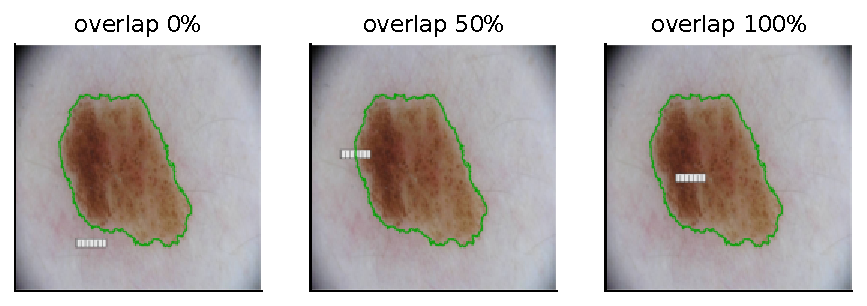
\includegraphics[width=\linewidth]{../stage1_problem_pilot_protocol/figures/ruler_examples.pdf}
\caption{The controlled sweep: the same ISIC 2018 image with the synthetic ruler at 0, 50 and 100\% overlap with the
lesion (\textcolor{roigreen}{green}: manual lesion mask). ISIC images CC BY-NC 4.0.}\label{s1:fig:ruler}\end{figure}
\begin{figure}[H]\centering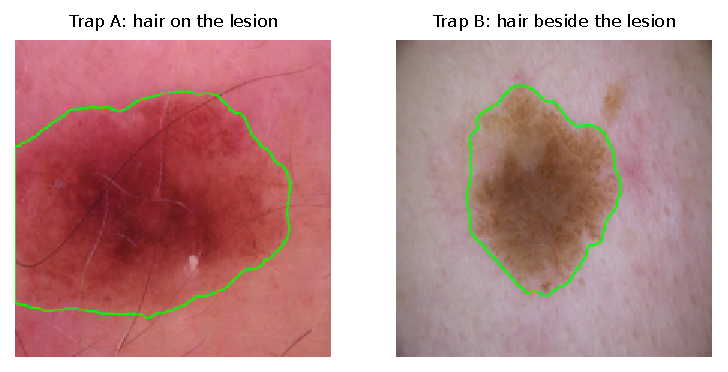
\includegraphics[width=0.78\linewidth]{../stage1_problem_pilot_protocol/figures/hair_examples.pdf}
\caption{The real hair traps (ISIC 2019): hair on the lesion (Trap~A) and beside it (Trap~B); the green line is the
lesion outline. The hair masks are not drawn because the published masks carry no licence that allows redistribution.
ISIC images CC BY-NC 4.0.}\label{s1:fig:hair}\end{figure}

\subsection{The protocol}
Table~\ref{s1:tab:protocol} lists every component with the reason it was chosen; Figure~\ref{s1:fig:env} shows the four test
environments.
\begin{table}[H]\centering\scriptsize
\caption{The protocol fixed in this stage.}\label{s1:tab:protocol}
\begin{tabular}{p{2.2cm}p{7.8cm}p{5.0cm}}\toprule
Component & Choice & Why \\\midrule
Environments & training and correlated test $P(A{=}1\mid Y{=}1)=0.9$, $P(A{=}1\mid Y{=}0)=0.1$; reversed test 0.1/0.9; clean test: no artifact (synthetic) or artifact independent of the label (real) & a strong, known shortcut whose use is exposed when the association is reversed \\
Primary metric & reversed-test AUROC; clean and correlated AUROC reported beside it & threshold-free; a model that uses the artifact must fall on the reversed test \\
Encoders & frozen DINOv2 ViT-B/14 at 518\,px (CLS token), DINOv2 at 224\,px, DermLIP (dermatology CLIP model) at 224\,px & how foundation models are used on small medical data; every arm sees the same features \\
Heads & logistic regression (liblinear, class-balanced); $C\in\{0.01,0.1,1,10\}$ and the decision threshold (maximal balanced accuracy) chosen on clean validation data only & no test or artifact information enters model selection \\
Arms & ERM; ROI masking; oracle inpainting of the artifact; group-balanced training; DFR; paired and unpaired LEACE; GroupDRO; prevalence calibration & masking is compared with methods that target the artifact itself \\
Splits & grouped by lesion identifier $\cup$ perceptual hash (Hamming $\le 8$); no group crosses a split & near-duplicates across a split inflate shortcut measurements (Sec.~\ref{s1:sec:leak}) \\
Seeds & 3 seeds (42, 123, 456) for the synthetic sweeps; 5 seeds $\times$ 5 grouped folds for the real hair traps & training and split variation are both part of the uncertainty \\
Uncertainty & crossed seed $\times$ image bootstrap, 10,000 replicates, percentile 95\% intervals & seeds share test images (Sec.~\ref{s1:sec:bootstrap}) \\
Registration & design, claims and support criteria committed to the repository before each verdict-producing run & separates confirmation from exploration \\
\bottomrule\end{tabular}
\end{table}

\begin{figure}[H]\centering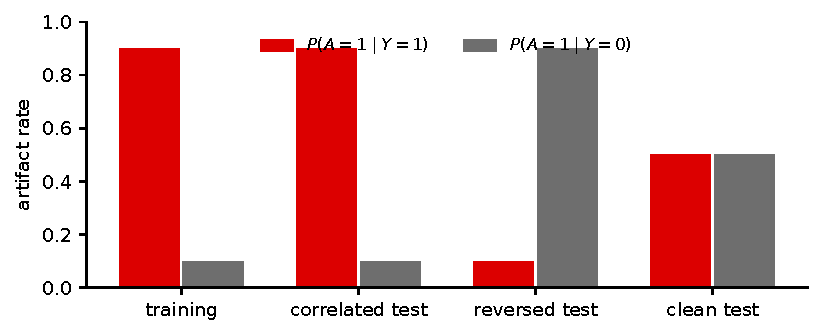
\includegraphics[width=0.78\linewidth]{../stage1_problem_pilot_protocol/figures/environments.pdf}
\caption{The trap environments. The training set and the correlated test share a strong artifact--label association;
the reversed test inverts it; the clean test removes it. A model that uses the artifact gains on the correlated test
and collapses on the reversed one.}\label{s1:fig:env}\end{figure}

\paragraph{Arms} \emph{ERM}: logistic head on the unmasked image. \emph{ROI masking}: pixels outside the lesion mask are
set to the image mean before feature extraction, at training and at test time. \emph{Oracle inpainting}: the known
artifact pixels are inpainted \citep{telea2004inpainting} --- an upper bound that needs the artifact mask.
\emph{Group-balanced}: the four artifact$\times$label cells are equally weighted. \emph{DFR}: the last layer is re-fitted
on a group-balanced subset of the validation fold \citep{kirichenko2023dfr}. \emph{LEACE}: closed-form linear erasure of
the artifact concept \citep{belrose2023leace}, either \emph{paired} (original versus artifact-removed versions of the
same images) or \emph{unpaired} (image-level artifact labels). \emph{GroupDRO} \citep{sagawa2020groupdro}.
\emph{Prevalence calibration} \citep{kina2026prevalence}. Balanced training, DFR, GroupDRO and unpaired LEACE need
image-level artifact labels; inpainting and paired LEACE need artifact masks; masking needs only the lesion mask.

\subsubsection{Leakage: grouped versus random splits}\label{s1:sec:leak}
Near-duplicate photographs of one lesion are common in ISIC. If one copy is in training and another in test, the test
measures memorisation. Every split therefore groups images by lesion identifier and perceptual hash (64-bit pHash,
Hamming distance $\le8$) and checks that no group crosses a split. To measure what this protects against, the
controlled sweep was repeated with five random image-level splits, everything else fixed.
\paragraph{Result} Random splits leave near-duplicate images on both sides of the split and inflate the measured ERM shortcut gap by 18\% (no overlap) and 10\% (full overlap), and shift both masking effects (Table~\ref{s1:tab:leak}); every analysis therefore uses grouped splits.%

\begin{table}[H]\centering\small
\caption{Leakage: grouped versus random image-level splits (controlled sweep, DINOv2@518).}\label{s1:tab:leak}
\resizebox{\linewidth}{!}{\begin{tabular}{lcccc}\toprule
Overlap & Split & Near-duplicate pairs across split & ERM gap (corr $-$ rev) & mask $-$ ERM (rev) \\\midrule
0\% & grouped & 0 & 0.241 & $+0.184$ \\
 & random (mean of 5) & 93 & 0.284 & $+0.223$ \\
100\% & grouped & 0 & 0.421 & $-0.129$ \\
 & random (mean of 5) & 93 & 0.465 & $-0.088$ \\
\bottomrule\end{tabular}}
\end{table}


\subsubsection{Uncertainty: the corrected (crossed) bootstrap}\label{s1:sec:bootstrap}
Every comparison is a paired difference in AUROC between two arms on the same test images, averaged over training
seeds (or cross-validation folds). The pilot's estimator resampled the seeds and then, \emph{independently within each
sampled seed}, the test images. In these designs, however, every seed scores the \emph{same} test images: the
controlled sweep uses one fixed test split, and in the hair traps the pooled cross-validation folds of every seed cover
the same image pool. Resampling the images independently per seed then treats one test set as several and divides the
test-sampling variance by the number of seeds, so the intervals are too narrow.
\paragraph{Why it matters} With three seeds and one test set, the per-seed estimator behaves as if the test set were
three times larger than it is. The problem is not specific to this project: any study that averages several training
seeds on one test set and resamples the images per seed has it.
\paragraph{The crossed estimator} Each replicate resamples the seeds with replacement and draws one Poisson(1) weight
per test \emph{image}, shared by every seed (and both arms) in which that image appears; the per-seed statistic is
recomputed with those weights and averaged (\texttt{wtss.stats\_crossed}; 10,000 replicates; percentile intervals).
The image weights make the test-set variance count once, as it should; the seed resampling keeps the training
variance. The estimator was registered before any interval was recomputed (\sOneRegCrossed; applied everywhere under
\sOneRegFinal).
\paragraph{Consequences for the pilot} On the \sOneCorrRows{} pilot intervals that both estimators can compute, the
crossed interval is wider by a median factor of \sOneCorrMedian{} (interquartile range \sOneCorrQlo--\sOneCorrQhi;
Figure~\ref{s1:fig:width}, Table~\ref{s1:tab:estcheck}). \sOneCorrLost{} intervals that excluded zero with the pilot's
estimator no longer do, and \sOneCorrGained{} now excludes zero (Table~\ref{s1:tab:estchanges}). Point estimates are
identical: only the uncertainty changed.
\begin{figure}[H]\centering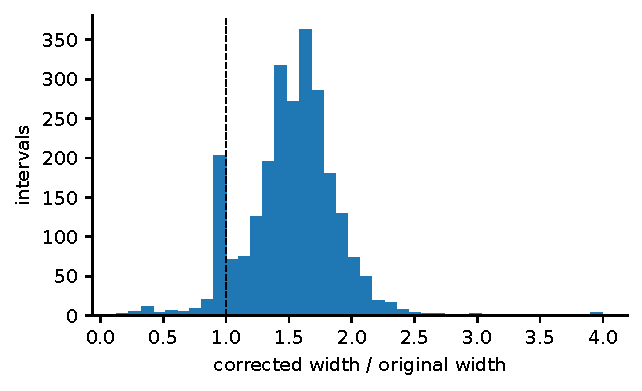
\includegraphics[width=0.58\linewidth]{../stage1_problem_pilot_protocol/figures/width_ratio.pdf}
\caption{Width of the crossed interval divided by the width of the pilot's per-seed interval, for every pilot
contrast (same predictions).}\label{s1:fig:width}\end{figure}
\begin{table}[H]\centering\scriptsize
\caption{The pilot's analyses under both interval estimators (same predictions, same point estimates; 10,000 replicates each). Width ratio $>1$: the crossed interval is wider.}\label{s1:tab:estcheck}
\begin{tabular}{p{5.0cm}p{1.4cm}p{2.6cm}p{2.6cm}p{2.4cm}}\toprule
Result group & Intervals & Excluded 0 only with the per-seed estimator & Excluded 0 only with the crossed estimator & Median width ratio (crossed / per-seed) \\\midrule
analysis/\allowbreak{}E14\_area\_ratio & 4 & 0 & 0 & 1.63 \\
spec\_e13/\allowbreak{}dermlip224\_spec & 29 & 1 & 0 & 1.45 \\
spec\_e13/\allowbreak{}dino518\_e12\_contrast & 3 & 0 & 0 & 1.44 \\
spec\_e13/\allowbreak{}dino518\_spec & 28 & 0 & 1 & 1.54 \\
synthetic/\allowbreak{}isic2018 & 114 & 6 & 0 & 1.44 \\
\textbf{all} & 178 & 7 & 1 & 1.45 \\
\bottomrule\end{tabular}
\end{table}

\begin{table}[H]\centering\scriptsize
\caption{The pilot contrasts whose verdict (interval excludes 0 or not) depends on the estimator. Every other contrast keeps its verdict.}\label{s1:tab:estchanges}
\begin{tabular}{p{4.2cm}p{5.2cm}p{3.3cm}p{2.6cm}}\toprule
Result & Contrast & Crossed estimate [95\% CI] & Verdict vs per-seed estimator \\\midrule
synthetic/\allowbreak{}isic2018/\allowbreak{}dino518\_ruler\_fixed\_corr\_main & 0.25 /\allowbreak{} mask /\allowbreak{} erm /\allowbreak{} test\_rev & $-0.059$ [$-0.127, +0.008$] & no longer excludes 0 \\
synthetic/\allowbreak{}isic2018/\allowbreak{}dino518\_ruler\_fixed\_occlusion\_occlusion & 0.0 /\allowbreak{} mask /\allowbreak{} erm /\allowbreak{} test\_uncorr & $+0.036$ [$-0.016, +0.086$] & no longer excludes 0 \\
synthetic/\allowbreak{}isic2018/\allowbreak{}dino518\_ruler\_fixed\_occlusion\_occlusion & 0.5 /\allowbreak{} mask /\allowbreak{} erm /\allowbreak{} test\_uncorr & $+0.041$ [$-0.010, +0.090$] & no longer excludes 0 \\
synthetic/\allowbreak{}isic2018/\allowbreak{}dino518\_ruler\_fixed\_occlusion\_occlusion & 0.75 /\allowbreak{} mask /\allowbreak{} erm /\allowbreak{} test\_uncorr & $+0.037$ [$-0.013, +0.086$] & no longer excludes 0 \\
synthetic/\allowbreak{}isic2018/\allowbreak{}dino518\_ruler\_fixed\_occlusion\_occlusion & 1.0 /\allowbreak{} mask /\allowbreak{} erm /\allowbreak{} test\_uncorr & $+0.039$ [$-0.010, +0.091$] & no longer excludes 0 \\
synthetic/\allowbreak{}isic2018/\allowbreak{}dino224\_ruler\_fixed\_corr\_main & 0.25 /\allowbreak{} mask /\allowbreak{} erm /\allowbreak{} test\_rev & $-0.049$ [$-0.117, +0.018$] & no longer excludes 0 \\
spec\_e13/\allowbreak{}dino518\_spec & trapA /\allowbreak{} mask /\allowbreak{} clean /\allowbreak{} all /\allowbreak{} mask /\allowbreak{} erm & $-0.023$ [$-0.045, -0.001$] & now excludes 0 \\
spec\_e13/\allowbreak{}dermlip224\_spec & trapB /\allowbreak{} leace\_unpaired /\allowbreak{} clean /\allowbreak{} all /\allowbreak{} leace\_unpaired /\allowbreak{} erm & $-0.019$ [$-0.046, +0.007$] & no longer excludes 0 \\
\bottomrule\end{tabular}
\end{table}


\subsubsection{Pre-registration}
Before every verdict-producing experiment, a document stating the design, the claims and what counts as support is
committed to the repository; results are committed afterwards, and a claim is reported whichever way it goes. The
pilot itself preceded this rule; its written specification (\texttt{docs/REPLICATION\_SPEC.md}, first commit
\sOneRegRep) serves as its registration for the replication. \textbf{Caveat:} commit times are set by the machine that
makes the commit and are not independent proof of order; registrations that are also pushed to GitHub before running
carry GitHub's time stamp as an external reference.

\subsection{The pilot and its re-implementation}
\subsubsection{What the pilot tested}
\posthoc{the pilot preceded pre-registration; its specification was written down afterwards and re-implemented}.
Table~\ref{s1:tab:pilot} lists the fifteen experiments. The pilot made five claims: (i) masking removes an artifact that
lies outside the lesion and makes the model worse than doing nothing when it lies inside; (ii) the harm is governed by
how much of the artifact survives the mask (retention), not by occlusion or lost context; (iii) methods that need
only an image-level artifact label (balanced training, DFR) fix both cases; (iv) linear erasure is insufficient for
real artifacts under the sound (paired) protocol; (v) all of this holds for real hair with pre-registered criteria on
two encoders.
\begin{table}[H]\centering\small
\caption{The pilot experiments (specification: \texttt{docs/REPLICATION\_SPEC.md}).}\label{s1:tab:pilot}
\begin{tabular}{lp{13cm}}\toprule
Exp. & What it tests \\\midrule
E1 & controlled ruler sweep, DINOv2@518: mask $-$ ERM at 0--100\% overlap; location interaction \\
E2 & the same at 224\,px (DINOv2) and with the dermatology model DermLIP \\
E3 & appearance randomisation (colour, opacity, ticks, scale of the ruler) \\
E4 & occlusion control: ruler present but uncorrelated with the label (50/50) \\
E5 & mask dilation: restoring ruler pixels around the lesion (retention) \\
E6 & same-head counterfactual sensitivity $|\Delta p|$ to inserting the ruler \\
E7 & lesion-size strata (artifact-to-lesion area ratio) \\
E8 & oracle inpainting and a prediction-consistency repair \\
E9 & bridge: group-balanced training, DFR, GroupDRO, paired LEACE at 100\% overlap \\
E10 & hair decodability from the embedding; paired LEACE on real hair \\
E11 & atlas of real artifacts (hair, ink, vignetting) in ISIC 2019 / HAM10000; vignetting trap \\
E12 & overlap-contrast trap: in-lesion versus out-of-lesion hair, no artifact-free group \\
E13 & real hair traps (Trap A in-lesion, Trap B out-of-lesion, shared hair-free group), ISIC 2019 \\
E14 & area-ratio strata of the real hair trap \\
E15 & E13 with DermLIP \\
\bottomrule\end{tabular}
\end{table}


\subsubsection{How it was re-implemented}
\registered{specification \texttt{docs/REPLICATION\_SPEC.md}, \sOneRegRep}. The pilot's code was not available for
most experiments (E9--E15), so every experiment was re-implemented from the written specification in a new code base
(\texttt{src/wtss}). A number \emph{matches} (MATCH) if it has the same sign, the same verdict on whether its interval
excludes zero, and differs by at most 0.02; SIGN+CI if sign and verdict agree but the difference is larger; MISMATCH
otherwise. Where the specification was silent or impossible to follow, the choice made is recorded with its reason
(Table~\ref{s1:tab:dev}). Two choices matter most: the hair-free group was defined as at most 30 hair pixels in the native
mask --- the only threshold that reproduces the pilot's outcome-free cell counts --- and, on the full ISIC 2019
cohort, pHash distance $\le8$ chains unrelated lesions into one giant component, so the real-hair traps apply it within
each trap pool, as the pilot's counts imply.
\begin{table}[H]\centering\scriptsize
\caption{Where the re-implementation deviates from the pilot's written specification, and why.}\label{s1:tab:dev}
\begin{tabular}{lp{3.0cm}p{4.6cm}p{7.0cm}}\toprule
\# & Specification & Re-implementation & Reason and effect \\\midrule
1 & GPU V100 32 GB & RTX 3090 24 GB & Frozen features; per-seed AUROCs of the rerun match the archive within 0.0005 (E1, E8, E9). \\
2 & Feature extraction per (seed, env) & per *view* (image $\times$ method $\times$ overlap), environments assembled by indexing & Mathematically identical (presence is a function of image/label/seed/env only); $\sim$10$\times$ fewer backbone passes. \\
3 & pHash $\le$ 8 on the full ISIC 2019 cohort (repo-default analysis) & spec E13 run: pHash $\le$ 8 within each matched trap pool (as the spec's counts imply); exploratory runs: lesion\_id $\cup$ pHash $\le$ 2 on all 25,331 & On all 25,331 images pHash $\le$ 8 chains unrelated lesions into one component of 10,974 images (same-lesion precision at distance 8: 2\%). \\
4 & Hair-free A = 0 group (threshold not stated in spec) & $\le$ 30 hair/ruler pixels in the native-resolution archive mask & Calibrated on outcome-free counts only: reproduces A0\_Y0 709 (spec 708), A0\_Y1 157 (157) and all six source proportions to 3 decimals. \\
5 & Archive mask file names & matched on zero-padded numeric id & Archive names are irregular (\_downsampled\_mvig, \_downsam\_inkmark, typos, truncated ids). 24 truncated ink ids flag their 10 candidate images as ink-uncertain (exploratory runs only). \\
6 & Images without HAM/BCN lesion\_id & source = MSK & Spec lists three sources; ISIC 2019's non-HAM/BCN images are MSK (incl. \_downsampled). \\
7 & U-Net (Ronneberger 64--1024, Task 1 only) & same architecture (+BatchNorm), 256 px, 40 epochs, Adam 1e-4, BCE+Dice, 20\% held-out pHash groups & Training hyper-parameters are not in the spec. \\
8 & Derm1M from archive & fresh clone of the official repo & Archived copy lacks bpe\_simple\_vocab\_16e6.txt.gz (.gz files were not archived); DermLIP cannot load without it. \\
9 & §3.1 "leakage inflated the gap by 27\%" & not reproduced from the archive & Pre-correction pilot used the identical split; matched-resolution gap ratio 0.96--0.97. A controlled leakage experiment is run instead (scripts/run\_leakage\_experiment.py). \\
\bottomrule\end{tabular}
\end{table}


\subsection{Results}
\subsubsection{Replication overview}
Of the \sOneNewN{} numbers the pilot reported, \sOneNewMatch{} MATCH, \sOneNewSignCI{} agree in sign and
significance but differ by more than 0.02, and \sOneNewMismatch{} MISMATCH (Table~\ref{s1:tab:ledger}). Before the
interval estimator was corrected the ledger read \sOneOrigMatch{} / \sOneOrigSignCI{} / \sOneOrigMismatch{} of
\sOneOrigN; the difference is entirely due to the wider intervals (Section~\ref{s1:sec:mismatch}).
{\scriptsize
\begin{longtable}{llp{1.7cm}p{3.3cm}l}
\caption{Replication ledger: every number the pilot reported, its re-derived value with the crossed 95\% interval, and the verdict. The pilot's own intervals came from the per-seed estimator (Sec.~\ref{s1:sec:bootstrap}) and are not reproduced; only its point values are shown.}\label{s1:tab:ledger}\\\toprule
Exp. & Quantity & Pilot (point) & Replication (crossed CI) & Verdict \\\midrule
\endfirsthead
\toprule Exp. & Quantity & Pilot (point) & Replication (crossed CI) & Verdict \\\midrule
\endhead
\bottomrule
\endlastfoot
E1 & mask $-$ ERM rev @0\% & +0.184 & +0.184 [+0.117, +0.250] & MATCH \\
E1 & mask $-$ ERM rev @25\% & -0.058 & -0.059 [-0.127, +0.008] & MISMATCH \\
E1 & mask $-$ ERM rev @50\% & -0.097 & -0.097 [-0.164, -0.030] & MATCH \\
E1 & mask $-$ ERM rev @75\% & -0.111 & -0.111 [-0.181, -0.043] & MATCH \\
E1 & mask $-$ ERM rev @100\% & -0.128 & -0.129 [-0.195, -0.064] & MATCH \\
E1 & interaction 0\% $-$ 100\% (mask) & +0.312 & +0.313 [+0.258, +0.370] & MATCH \\
E2 & dino224 mask $-$ ERM @0\% & +0.364 & +0.361 [+0.275, +0.444] & MATCH \\
E2 & dino224 mask $-$ ERM @25\% & -0.040 & -0.049 [-0.117, +0.018] & MATCH \\
E2 & dino224 mask $-$ ERM @50\% & -0.076 & -0.081 [-0.143, -0.019] & MATCH \\
E2 & dino224 mask $-$ ERM @75\% & -0.102 & -0.106 [-0.166, -0.044] & MATCH \\
E2 & dino224 mask $-$ ERM @100\% & -0.092 & -0.095 [-0.156, -0.035] & MATCH \\
E2 & dermlip224 mask $-$ ERM @0\% & +0.160 & +0.161 [+0.102, +0.222] & MATCH \\
E2 & dermlip224 mask $-$ ERM @25\% & -0.291 & -0.289 [-0.366, -0.215] & MATCH \\
E2 & dermlip224 mask $-$ ERM @50\% & -0.300 & -0.298 [-0.371, -0.225] & MATCH \\
E2 & dermlip224 mask $-$ ERM @75\% & -0.313 & -0.309 [-0.378, -0.239] & MATCH \\
E2 & dermlip224 mask $-$ ERM @100\% & -0.268 & -0.263 [-0.348, -0.180] & MATCH \\
E3 & variable ruler mask $-$ ERM @0\% & +0.147 & +0.146 [+0.082, +0.211] & MATCH \\
E3 & variable ruler mask $-$ ERM @50\% & -0.094 & -0.094 [-0.168, -0.021] & MATCH \\
E3 & variable ruler mask $-$ ERM @100\% & -0.155 & -0.155 [-0.228, -0.084] & MATCH \\
E3 & variable ruler balanced $-$ ERM @0\% & +0.103 & +0.102 [+0.068, +0.140] & MATCH \\
E3 & variable ruler balanced $-$ ERM @50\% & +0.171 & +0.171 [+0.132, +0.213] & MATCH \\
E3 & variable ruler balanced $-$ ERM @100\% & +0.222 & +0.222 [+0.181, +0.265] & MATCH \\
E4 & occlusion (50/50) mask $-$ ERM @0\% & +0.035 & +0.036 [-0.016, +0.086] & MISMATCH \\
E4 & occlusion (50/50) mask $-$ ERM @50\% & +0.033 & +0.041 [-0.010, +0.090] & MATCH \\
E4 & occlusion (50/50) mask $-$ ERM @100\% & +0.039 & +0.039 [-0.010, +0.091] & MISMATCH \\
E5 & dilate0 $-$ ERM @50\% & -0.097 & -0.097 [-0.164, -0.031] & MATCH \\
E5 & dilate10 $-$ ERM @50\% & -0.138 & -0.138 [-0.203, -0.074] & MATCH \\
E5 & dilate25 $-$ ERM @50\% & -0.153 & -0.153 [-0.221, -0.089] & MATCH \\
E5 & dilate50 $-$ ERM @50\% & -0.142 & -0.142 [-0.206, -0.083] & MATCH \\
E5 & dilate0 $-$ ERM @100\% & -0.128 & -0.129 [-0.195, -0.066] & MATCH \\
E5 & dilate10 $-$ ERM @100\% & -0.143 & -0.144 [-0.206, -0.082] & MATCH \\
E5 & dilate25 $-$ ERM @100\% & -0.144 & -0.144 [-0.209, -0.082] & MATCH \\
E5 & dilate50 $-$ ERM @100\% & -0.138 & -0.138 [-0.200, -0.082] & MATCH \\
E6 & $|\Delta p|$ erm @100\% & +0.235 & +0.235 & MATCH \\
E6 & $|\Delta p|$ mask @100\% & +0.490 & +0.491 & MATCH \\
E6 & $|\Delta p|$ mask @0\% & +0.000 & +0.000 & MATCH \\
E6 & $|\Delta p|$ erm @0\% & +0.128 & +0.128 & MATCH \\
E6 & $|\Delta p|$ erm @50\% & +0.195 & +0.195 & MATCH \\
E7 & mask $-$ ERM, large lesions @0\% & +0.249 & +0.249 & MATCH \\
E7 & mask $-$ ERM, medium lesions @0\% & +0.214 & +0.215 & MATCH \\
E7 & mask $-$ ERM, small lesions @0\% & +0.150 & +0.150 & MATCH \\
E7 & mask $-$ ERM, large lesions @50\% & +0.087 & +0.087 & MATCH \\
E7 & mask $-$ ERM, medium lesions @50\% & -0.129 & -0.129 & MATCH \\
E7 & mask $-$ ERM, small lesions @50\% & -0.325 & -0.326 & MATCH \\
E7 & mask $-$ ERM, large lesions @100\% & +0.064 & +0.063 & MATCH \\
E7 & mask $-$ ERM, medium lesions @100\% & -0.158 & -0.158 & MATCH \\
E7 & mask $-$ ERM, small lesions @100\% & -0.364 & -0.364 & MATCH \\
E14 & in-lesion hair median area ratio & +0.033 & +0.033 & MATCH \\
E14 & Trap A mask $-$ ERM, area-ratio tertile T1 & -0.064 & -0.057 [-0.095, -0.022] & MATCH \\
E14 & Trap A mask $-$ ERM, area-ratio tertile T2 & -0.057 & -0.046 [-0.082, -0.013] & MATCH \\
E14 & Trap A mask $-$ ERM, area-ratio tertile T3 & -0.059 & -0.037 [-0.071, -0.005] & SIGN+CI \\
E10 & hair decodability test AUROC & +0.943 & +0.943 [+0.919, +0.964] & MATCH \\
E10 & detector mean IoU & +0.220 & +0.222 & MATCH \\
E10 & detector median IoU & +0.180 & +0.184 & MATCH \\
E10 & LEACE A-decoder after erasure & +0.500 & +0.500 & MATCH \\
E10 & clean melanoma AUROC after erasure & +0.814 & +0.815 & MATCH \\
E10 & melanoma-head $|\Delta p|$ after erasure & +0.058 & +0.057 & MATCH \\
E10 & LEACE projection rank & +1.000 & +1.000 & MATCH \\
E12 & overlap-contrast trap mask $-$ ERM (spec: null) & +0.047 & -0.103 [-0.121, -0.085] & MISMATCH \\
E8/E9 & inpaint $-$ ERM @50\% & +0.211 & +0.211 [+0.175, +0.249] & MATCH \\
E8/E9 & inpaint $-$ ERM @100\% & +0.244 & +0.243 [+0.205, +0.284] & MATCH \\
E8/E9 & inpaint\_consistency $-$ ERM @50\% & +0.046 & +0.044 [-0.007, +0.092] & MATCH \\
E8/E9 & inpaint\_consistency\_lam0 $-$ ERM @50\% & +0.036 & +0.035 [-0.015, +0.086] & MATCH \\
E8/E9 & leace $-$ ERM @100\% & +0.294 & +0.294 [+0.249, +0.339] & MATCH \\
E8/E9 & balanced $-$ ERM @100\% & +0.281 & +0.281 [+0.236, +0.329] & MATCH \\
E8/E9 & dfr $-$ ERM @100\% & +0.279 & +0.279 [+0.220, +0.339] & MATCH \\
E8/E9 & groupdro $-$ ERM @100\% & +0.197 & +0.197 [+0.155, +0.240] & MATCH \\
E13 & trapA mask $-$ ERM (rev) & -0.064 & -0.049 [-0.083, -0.018] & MATCH \\
E13 & trapB mask $-$ ERM (rev) & +0.124 & +0.098 [+0.060, +0.136] & SIGN+CI \\
E13 & trapA inpaint $-$ ERM (rev) & +0.101 & +0.098 [+0.084, +0.112] & MATCH \\
E13 & trapB inpaint $-$ ERM (rev) & +0.108 & +0.100 [+0.083, +0.117] & MATCH \\
E13 & trapA balanced $-$ ERM (rev) & +0.213 & +0.213 [+0.183, +0.243] & MATCH \\
E13 & trapB balanced $-$ ERM (rev) & +0.234 & +0.204 [+0.166, +0.245] & SIGN+CI \\
E13 & trapA dfr $-$ ERM (rev) & +0.202 & +0.196 [+0.157, +0.235] & MATCH \\
E13 & trapB dfr $-$ ERM (rev) & +0.192 & +0.196 [+0.147, +0.251] & MATCH \\
E13 & trapA leace\_paired $-$ ERM (rev) & +0.058 & +0.074 [+0.062, +0.086] & MATCH \\
E13 & trapB leace\_paired $-$ ERM (rev) & +0.078 & +0.078 [+0.059, +0.097] & MATCH \\
E13 & trapA leace\_unpaired $-$ ERM (rev) & +0.316 & +0.320 [+0.280, +0.361] & MATCH \\
E13 & trapA mask $-$ ERM, HAM only & -0.030 & -0.011 [-0.064, +0.043] & MISMATCH \\
E13 & trapA mask $-$ ERM, BCN only & -0.078 & -0.067 [-0.110, -0.025] & MATCH \\
E15 & trapA mask $-$ ERM (rev) & -0.069 & -0.104 [-0.143, -0.067] & SIGN+CI \\
E15 & trapA balanced $-$ ERM (rev) & +0.126 & +0.146 [+0.122, +0.170] & MATCH \\
E15 & trapA dfr $-$ ERM (rev) & +0.114 & +0.116 [+0.090, +0.145] & MATCH \\
E15 & trapA leace\_paired $-$ ERM (rev) & +0.031 & +0.034 [+0.026, +0.042] & MATCH \\
E15 & trapA leace\_unpaired $-$ ERM (rev) & +0.192 & +0.203 [+0.165, +0.243] & MATCH \\
\end{longtable}}


\subsubsection{The controlled sweep (E1--E3, E8--E9)}
\begin{figure}[H]\centering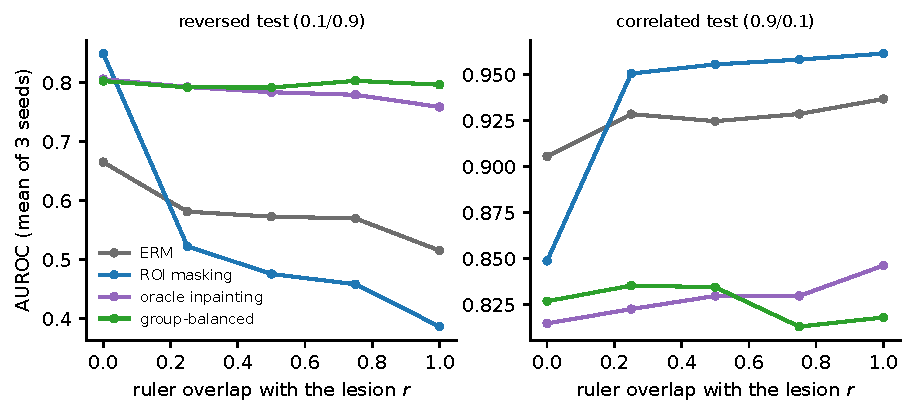
\includegraphics[width=\linewidth]{../stage1_problem_pilot_protocol/figures/pilot_sweep.pdf}
\caption{The pilot's central result, re-derived: reversed-test (left) and correlated-test (right) AUROC of four arms as
the ruler moves into the lesion (ISIC 2018, DINOv2 @518, mean of 3 seeds). Masking helps most when the ruler lies
outside the lesion and falls below ERM once it overlaps it; its correlated-test AUROC rises with overlap --- the
masked model relies on the ruler it can still see.}\label{s1:fig:pilotsweep}\end{figure}
Masking changes the reversed-test AUROC by \sOneEOneZero{} when the ruler lies outside the lesion and by
\sOneEOneHundred{} when it lies fully inside; the location interaction is \sOneEOneInter{} (Figure~\ref{s1:fig:pilotsweep}).
Two numbers show what happens. At 0\% overlap the masked model's correlated and reversed AUROC coincide
(\sOneAucmasktestcorrZeroZero{} and \sOneAucmasktestrevZeroZero): the ruler has been removed and nothing of the
shortcut remains. At 100\% overlap the masked model's correlated AUROC (\sOneAucmasktestcorrOneZero) is \emph{higher}
than ERM's (\sOneAucermtestcorrOneZero) while its reversed AUROC collapses to \sOneAucmasktestrevOneZero{} (ERM
\sOneAucermtestrevOneZero): after masking, the model uses the ruler \emph{more}.

The reversal is not a property of one encoder or one rendering. At 224\,px DINOv2 gives \sOneDinoTTFZero{} and
\sOneDinoTTFFull{} (interaction \sOneDinoTTFInter); the dermatology model DermLIP gives \sOneDermlipZero{} and
\sOneDermlipFull{} (\sOneDermlipInter); a ruler whose colour, opacity, tick pattern and scale are randomised per image
gives an interaction of \sOneStressInter.

Methods that target the artifact rather than the background all help at full overlap: oracle inpainting
\sOneSwinpaintOneZero, group balancing \sOneSwbalancedOneZero, DFR \sOneSwdfrOneZero, LEACE \sOneSwleaceOneZero{} and
GroupDRO \sOneSwgroupdroOneZero. A training-time repair that asks the model to give the same prediction with and
without the ruler (``consistency'', E8) gives \sOneSwinpaintconsistencyZeroFive{} at 50\% overlap, and \sOneSwinpaintconsistencylamZeroZeroFive{}
without its penalty ($\lambda=0$): neither is significant, and the penalty adds nothing to the augmentation.

\paragraph{The pilot's mechanism experiments (E4--E7)} replicate numerically (Table~\ref{s1:tab:ledger}): with the ruler
present but uninformative, masking does not harm (E4); dilating the mask so that more ruler pixels survive increases
the harm at 50\% overlap (E5); the masked model's prediction reacts about twice as strongly to inserting the ruler as
ERM's at full overlap (E6); and the harm is largest for small lesions (E7). What these observations imply about the
mechanism is not interpreted in this stage; only their reproducibility is.

\subsubsection{Real hair (E10, E12--E15)}
\paragraph{Cohort} Under the specification's rules the matched cells are: hair-free group \sOneCnttrapAAZeroYZero{}
benign / \sOneCnttrapAAZeroYOne{} melanoma (pilot \sOneExptrapAAZeroYZero{} / \sOneExptrapAAZeroYOne); Trap~A hair-bearing
\sOneCnttrapAAOneYZero{} / \sOneCnttrapAAOneYOne{} (pilot \sOneExptrapAAOneYZero{} / \sOneExptrapAAOneYOne); Trap~B
\sOneCnttrapBAOneYZero{} / \sOneCnttrapBAOneYOne{} (pilot \sOneExptrapBAOneYZero{} / \sOneExptrapBAOneYOne); \sOneRevMeltrapA{}
reversed-test melanomas per trap and seed, as in the pilot. The hair-free cells reproduce the pilot's counts; the
hair-bearing cells differ by 5--15\% because the lesion masks of non-HAM images come from a re-trained U-Net, which
moves some images across the overlap thresholds (a swap of mask source changes the overlap stratum of 6.9\% of
hair-bearing images and moves none from Trap~A to Trap~B).

\paragraph{E13 (DINOv2@518)} Table~\ref{s1:tab:e13dino}. Masking \emph{harms} when the hair lies on the lesion
(\sOneAdino) and helps when it lies beside it (\sOneBdino); the crossover is \sOneXdino. The masked Trap-A model still
separates the correlated test (0.917) far better than the reversed one (0.460): it uses the hair it can still see.
Every artifact-targeting arm helps in both traps; group balancing and DFR, which need only image-level hair labels,
help most (C4). Paired LEACE recovers about a third of the balanced gain (C5). Unpaired LEACE ``helps'' by
\emph{flipping} the shortcut --- its correlated AUROC (0.624) falls far below its reversed one (0.830) --- which is why
the pilot rejected it as unsound. The harm is concentrated in BCN images (\sOneSrcdinoBCN; HAM \sOneSrcdinoHAM).
Masking also costs clean-test AUROC in Trap~A (\sOneACleandino).
\begin{table}[H]\centering\scriptsize
\caption{Real hair traps (DINOv2@518; E13): AUROC in the three test environments (mean over 5 seeds) and change in reversed-test AUROC versus ERM (crossed 95\% CI). Trap A: hair on the lesion; Trap B: hair beside it; both share the hair-free group.}\label{s1:tab:e13dino}
\resizebox{\linewidth}{!}{\begin{tabular}{p{3.2cm}cccc}\toprule
Arm & Trap A: clean / corr / rev & Trap A: $\Delta$ rev vs ERM & Trap B: clean / corr / rev & Trap B: $\Delta$ rev vs ERM \\\midrule
ERM & 0.734 / 0.920 / 0.510 & --- & 0.716 / 0.894 / 0.510 & --- \\
ROI masking & 0.712 / 0.917 / 0.460 & $-0.049$ [$-0.083, -0.018$] & 0.701 / 0.795 / 0.608 & $+0.098$ [$+0.060, +0.136$] \\
oracle inpainting of hair & 0.766 / 0.906 / 0.607 & $+0.098$ [$+0.084, +0.112$] & 0.738 / 0.865 / 0.610 & $+0.100$ [$+0.083, +0.117$] \\
group-balanced & 0.785 / 0.850 / 0.722 & $+0.213$ [$+0.183, +0.243$] & 0.752 / 0.800 / 0.714 & $+0.204$ [$+0.166, +0.245$] \\
DFR & 0.715 / 0.740 / 0.705 & $+0.196$ [$+0.157, +0.235$] & 0.683 / 0.669 / 0.706 & $+0.196$ [$+0.147, +0.251$] \\
paired LEACE & 0.762 / 0.913 / 0.584 & $+0.074$ [$+0.062, +0.086$] & 0.737 / 0.876 / 0.588 & $+0.078$ [$+0.059, +0.097$] \\
unpaired LEACE (image-level $A$) & 0.726 / 0.624 / 0.830 & $+0.320$ [$+0.280, +0.361$] & \na & \na \\
\bottomrule\end{tabular}}
\end{table}

\paragraph{E15 (DermLIP@224)} Table~\ref{s1:tab:e13dermlip}. Masking harms in Trap~A (\sOneAdermlip) as the pilot
reported, but --- a finding the pilot did not test --- it harms in Trap~B as well (\sOneBdermlip), so DermLIP shows no
crossover (\sOneXdermlip). With DermLIP, removing the background costs disease signal wherever the hair lies (clean
AUROC \sOneACleandermlip{} in Trap~A).
\begin{table}[H]\centering\scriptsize
\caption{Real hair traps (DermLIP@224; E13/E15): AUROC in the three test environments (mean over 5 seeds) and change in reversed-test AUROC versus ERM (crossed 95\% CI). Trap A: hair on the lesion; Trap B: hair beside it; both share the hair-free group.}\label{s1:tab:e13dermlip}
\resizebox{\linewidth}{!}{\begin{tabular}{p{3.2cm}cccc}\toprule
Arm & Trap A: clean / corr / rev & Trap A: $\Delta$ rev vs ERM & Trap B: clean / corr / rev & Trap B: $\Delta$ rev vs ERM \\\midrule
ERM & 0.801 / 0.917 / 0.665 & --- & \na & \na \\
ROI masking & 0.735 / 0.884 / 0.561 & $-0.104$ [$-0.143, -0.067$] & \na & \na \\
oracle inpainting of hair & \na & \na & \na & \na \\
group-balanced & 0.836 / 0.875 / 0.811 & $+0.146$ [$+0.122, +0.170$] & \na & \na \\
DFR & 0.802 / 0.835 / 0.782 & $+0.116$ [$+0.090, +0.145$] & \na & \na \\
paired LEACE & 0.814 / 0.917 / 0.699 & $+0.034$ [$+0.026, +0.042$] & \na & \na \\
unpaired LEACE (image-level $A$) & 0.756 / 0.648 / 0.868 & $+0.203$ [$+0.165, +0.243$] & \na & \na \\
\bottomrule\end{tabular}}
\end{table}

\paragraph{E10: is hair visible to the encoder?} A linear probe decodes hair presence from the DINOv2 embedding with
AUROC \sOneHairDec{} ($n=\sOneHairDecN$ test images); in that set hair is \emph{less} common on melanomas
(\sOneHairPMel) than on benign lesions (\sOneHairPBen). Paired LEACE on \sOneLeaceN{} images with manual hair masks
(\sOneLeaceTrain{} training pairs) needs only one direction: the hair decoder falls from \sOneLeaceDecRaw{} to chance
(\sOneLeaceDecAfter), clean melanoma AUROC is unchanged (\sOneLeaceCleanRaw{} to \sOneLeaceCleanAfter), yet the
melanoma head's reaction to hair only falls from \sOneLeaceDpRaw{} to \sOneLeaceDpAfter. A classical morphological
hair detector (DullRazor-style) is poor: mean IoU \sOneDetIoU{} (median \sOneDetIoUMed; precision \sOneDetP, recall
\sOneDetR) --- which is why the real traps use the published masks rather than a detector.
\paragraph{E14: how large is real hair relative to the lesion?} In Trap~A the in-lesion hair covers a median
\sOneEFourteenMed{} of the lesion area, similar to the synthetic ruler. Masking harms in every tertile of this ratio
(\sOneEFourteenTOne, \sOneEFourteenTTwo, \sOneEFourteenTThree); the pilot's ``same harm at every ratio'' pattern
replicates, with the smallest harm in the tertile with the most hair.

\subsubsection{E12: the overlap-contrast design}\label{s1:sec:e12}
E12 labelled hair on the lesion as $A=1$ and hair beside it as $A=0$, with no hair-free group, and the pilot reported
a null result. The re-implementation finds masking clearly harmful (\sOneEOneTwomask), while balancing
(\sOneEOneTwobalanced) and DFR (\sOneEOneTwodfr) help. This is what the design predicts whatever the truth, because
in E12 location \emph{is} the label proxy: masking removes exactly the out-of-lesion hair that defines one side of the
contrast and keeps the in-lesion hair that defines the other. The design cannot measure a location effect; E13's
two traps with a shared hair-free group can. The pilot's null E12 result is not supported, and the design is not used
further.

\subsubsection{Audit of the pilot's written claims}
Besides the numbers, the pilot's report made statements that were checked against the archived material
(\texttt{docs/THESIS\_CLAIMS\_AUDIT.md}):
\begin{itemize}[leftmargin=*]\itemsep1pt
\item \textbf{``Leakage inflated the shortcut gap by 27\%''} --- \no\ as stated. The pre-correction pilot used the
identical split; the 27\% compared runs at different resolutions. The controlled experiment of
Section~\ref{s1:sec:leak} supports the direction with a magnitude of 10--18\%.
\item \textbf{Archived numbers} --- verified: all 21 bridge intervals of the controlled sweep were recomputed from the
archived predictions to $10^{-16}$, and a re-run from raw images reproduced 252 per-seed AUROCs within 0.0005 (a GPU
precision effect).
\item \textbf{Lesion U-Net} --- the pilot's U-Net code was missing and was re-implemented. The specification's
architecture, used for the hair traps, reaches a held-out Dice of 0.89 (pilot 0.88); a ResNet-34 U-Net used for
exploratory checks reaches 0.94.
\item \textbf{Mask-source sensitivity} --- the pilot reported that about 11\% of images change overlap stratum when the
mask source is swapped; the re-implementation finds 6.9\%, and no image moves between Trap~A and Trap~B.
\item \textbf{E11 (artifact atlas and vignetting trap)} was not re-implemented: ink appears on the lesion in too few
images (the traps exclude ink), and vignetting is a frame artifact that lies outside the lesion by construction, so it
cannot inform the in-ROI question.
\end{itemize}

\subsubsection{The mismatches}\label{s1:sec:mismatch}
\begin{enumerate}[leftmargin=*]\itemsep1pt
\item \textbf{E1, masking at 25\% overlap.} The pilot's interval excluded zero; the crossed interval includes it. The
harm is significant from 50\% overlap onward.
\item \textbf{E4, occlusion control at 0\% and 100\% overlap.} The pilot reported small positive effects of masking
with the ruler present but uninformative; with the crossed estimator they are not significant. The conclusion ---
occlusion by the mask does not harm --- is unchanged.
\item \textbf{E12.} Not null (above); a structural problem of the design.
\item \textbf{E13, HAM-only stratum.} The pilot reported harm in HAM images; the replication does not
(\sOneSrcdinoHAM). The harm is carried by BCN images.
\end{enumerate}
None of these affects the pilot's central claim --- that masking reverses from helpful to harmful as the ruler moves
into the lesion --- which replicates with every encoder and ruler rendering.

\subsection{What failed or changed in this stage}
\begin{itemize}[leftmargin=*]\itemsep1pt
\item The pilot's interval estimator was too narrow whenever seeds share test images; it was replaced, and three pilot
significance claims (E1 at 25\%, E4 at 0\% and 100\%) no longer hold.
\item E12's null result and the ``27\%'' leakage figure are not supported; the HAM-only harm of E13 does not replicate.
\item DermLIP shows no hair crossover in the replication: it is harmed by masking at both hair locations.
\item The hair-bearing cells of E13 differ by 5--15\% from the pilot's because the lesion U-Net had to be re-trained.
\end{itemize}

\subsection{Anticipated questions}
\paragraph{Why re-implement instead of re-running the pilot's code?} Most of the pilot's code for E9--E15 was not in
the archive, and re-running code verifies only that it runs. Re-implementing from a written specification tests
whether the \emph{description} is sufficient to reproduce the result, which is what a reader of a paper can do.
\paragraph{Why is the reversed test the primary metric, not the clean test?} The clean test measures disease
recognition without the shortcut, so it cannot show whether a model \emph{uses} the artifact. The reversed test
penalises reliance on the artifact directly. Both are always reported, together with the correlated test, so that a
method that simply inverts the shortcut (as unpaired LEACE does) is visible.
\paragraph{Why 0.9/0.1?} It is strong enough that every encoder learns the shortcut, which is the regime where
mitigation matters, and weak enough that both classes contain artifact-free and artifact-bearing images in training.
The same values are used everywhere, so effects are comparable.
\paragraph{Why frozen encoders and linear heads?} Every arm then uses identical features; differences between arms
are caused by the input (masked or not) or the head, not by optimisation noise. It is also the common way foundation
models are deployed on small medical datasets.
\paragraph{Why choose $C$ and the threshold on clean validation data?} Choosing them on data with the shortcut would
reward the shortcut; choosing them on reversed data would leak the test condition into training.
\paragraph{Why group by perceptual hash and not by patient?} ISIC 2018 does not publish patient identifiers; lesion
identifiers and near-duplicate detection are the strongest grouping available. The leakage experiment shows that this
grouping matters (10--18\% gap inflation otherwise).
\paragraph{Why a crossed bootstrap and not simply more seeds?} More seeds reduce training variance but do not create
new test images. The quantity of interest is a difference on a finite test set; its uncertainty must include the
sampling of that set once, which is what the shared image weights do.
\paragraph{Why do the E13 cell counts differ from the pilot's?} The hair-free group reproduces exactly. The
hair-bearing cells depend on the lesion masks of non-HAM images, which come from a re-trained U-Net; images near the
0.1 and 0.5 overlap thresholds move between strata. No image moves between Trap~A and Trap~B.
\paragraph{Why does unpaired LEACE look best, and why is it rejected?} It removes the direction that separates images
with and without hair \emph{in the training data}, where hair is strongly associated with the label; that direction
contains much of the diagnosis, and the model ends up predicting the opposite of the shortcut (correlated AUROC far
below reversed). Paired LEACE compares the same image with and without hair and removes only the hair.
\paragraph{Is 2,437 images enough?} For the controlled sweep, yes: the location interaction is large relative to its
interval (\sOneEOneInter). Individual overlap cells are less precise, which is why the 25\% cell lost significance.

\subsection{Conclusion}
\textbf{Supported.} The pilot's central result replicates from its written specification: masking helps when the
ruler lies outside the lesion and harms when it overlaps it (interaction \sOneEOneInter), with two encoders, two
resolutions and a randomised ruler; with real hair on DINOv2 masking harms in-lesion and helps out-of-lesion (crossover
\sOneXdino); methods that need only an image-level artifact label fix both traps; paired linear erasure is insufficient.
\textbf{Not supported.} The pilot's null E12 result; the ``27\%'' leakage figure; significance at 25\% overlap and in
the occlusion control; harm in HAM images; a hair crossover with DermLIP. \textbf{Fixed for the rest of the work.}
Grouped splits, clean-validation model selection, pre-registration, and the crossed bootstrap.

\subsection{Questions for the supervisor}
\begin{enumerate}\itemsep1pt
\item Is the reversed-environment AUROC acceptable as the primary metric for the thesis, or should a clinical metric
(sensitivity at a fixed specificity) be primary from the start?
\item How should the thesis present the estimator correction: as a methods detail, or as a contribution in its own
right (it affects any study that averages several training seeds on one test set)?
\item Should the E12 design and its failure be reported in the thesis (as a warning about contrast designs) or only in
the appendix?
\item Is it acceptable that the pilot's registration is its written specification, committed after the pilot ran?
\end{enumerate}


\clearpage
% generated by make_combined.py from stage2_location_law_mechanism/stage2.tex; do not edit
\section{Stage 2 --- The location law and its mechanism}\label{sec:stage2}

\stagebox{\textbf{In one sentence.} When only the artifact's overlap with the region of interest (ROI) is varied,
ROI masking helps while the artifact lies outside the ROI and loses its benefit --- in 7 of 11 sweeps it hurts ---
once the artifact overlaps it; the reversal comes from the artifact \emph{surviving} the mask and becoming what the model
relies on, not from occlusion; and it recurs in thyroid and ovarian ultrasound, capsule endoscopy and chest
radiography, with one principled exception (an encoder that ignores an artifact outside the lungs).}
\subsection{Where this stage starts}
Stage~1 re-derived the pilot and fixed the protocol: trap environments, frozen foundation-model features, linear heads
chosen on clean validation data, grouped splits, pre-registration and the crossed bootstrap. It showed that the
pilot's central observation replicates: in the controlled dermoscopy sweep, masking changes reversed-test AUROC from
\sTwoMaskZero{} at 0\% overlap to \sTwoMaskOneZeroZero{} at 100\% overlap. Stage~1 deliberately did not interpret the
pilot's mechanism experiments. This stage asks the two questions that follow: \emph{why} does masking reverse, and
\emph{how general} is the reversal --- does it depend on dermoscopy, on the ruler, on DINOv2?

\subsection{Questions}
\begin{enumerate}[label=\textbf{Q2\alph*},leftmargin=*]\itemsep1pt
\item Is the benefit of masking a function of the artifact's overlap $r$ with the ROI, falling from $r=0$ to $r=1$?
We call a positive location interaction $\big[\mathrm{mask}-\mathrm{ERM}\big]_{r=0}-\big[\mathrm{mask}-\mathrm{ERM}\big]_{r=1}$
on the reversed test the \emph{location law}.
\item Which mechanism produces the fall? Three candidates were stated in advance: \emph{occlusion} (masking removes
useful context whatever the artifact does), \emph{lost disease signal} (the background carries diagnostic
information), and \emph{retention with amplified reliance} (the part of the artifact inside the ROI survives masking,
its competitors are removed, and the head relies on it more).
\item Does the law hold beyond one encoder, one artifact rendering and one modality --- and where does it fail?
\end{enumerate}

\subsubsection{Why these experiments, and what was rejected}
\begin{itemize}[leftmargin=*]\itemsep1pt
\item \emph{An occlusion control instead of an argument from intuition.} If masking harmed because it throws away
context, it would harm even when the artifact carries no label information \citep[cf.][]{fong2019occlusions}. The
control keeps the ruler at the same positions but makes it independent of the label.
\item \emph{Dilation as a dose of retention.} Growing the mask by a margin keeps more of the ruler visible without
changing the lesion. If retention drives the harm, harm should grow with retention when retention is incomplete (50\%
overlap) and stay flat when the ruler is already fully retained (100\% overlap) --- even though dilation then
\emph{lowers} the ruler's share of the visible pixels.
\item \emph{A same-head counterfactual instead of saliency maps.} Saliency maps are qualitative and unstable for frozen
encoders. Instead, the ruler is inserted into and removed from the \emph{same} test image and the change in each
trained head's predicted probability, $|\Delta p|$, is read: a direct, per-image measure of reliance on the artifact.
\item \emph{Lesion size as a natural dose.} The same ruler covers a larger share of a small lesion. If what matters is
how dominant the retained artifact is among the remaining evidence, harm should be largest for small lesions. No
threshold ratio was pre-specified, because the pilot showed none.
\item \emph{Other modalities with their own artifact.} A caliper drawn like a sonographer's, a debris blob drawn like
capsule contamination and a tube drawn like a drain, each pasted at controlled overlap on real images of that modality
with that modality's own ROI masks. This tests whether the law is a property of dermoscopy or of masking.
\item \emph{Rejected:} measuring reliance through head weights (they are not comparable between masked and unmasked
feature spaces), and a single ``average'' overlap (it would hide the sign change).
\end{itemize}

\subsection{Methods}
\paragraph{Controlled dermoscopy sweep} As in Stage~1: ISIC 2018 pilot cohort, a $65\times19$\,px ruler at a frozen
position per image and overlap $r\in\{0,0.25,0.5,0.75,1\}$; DINOv2 ViT-B/14 at 518\,px \citep{oquab2024dinov2} (CLS
features), logistic heads, seeds 42, 123, 456; primary outcome reversed-test AUROC.
\paragraph{Arms} ERM; ROI masking; oracle inpainting of the ruler; group-balanced reweighting; DFR
\citep{kirichenko2023dfr}; paired LEACE \citep{belrose2023leace}; GroupDRO \citep{sagawa2020groupdro}. All arms share
features and seeds; only the input or the head changes.
\paragraph{Occlusion control} The ruler is pasted at the same positions in 50\% of images independently of the label;
AUROC is measured on a 50/50 test.
\paragraph{Mask dilation} The lesion mask is dilated by 0, 10, 25 or 50\,px before masking. \emph{Retention} is the share
of ruler pixels that remain visible; \emph{ruler share} is the ruler's share of all visible pixels.
\paragraph{Same-head counterfactual} For each artifact-bearing image of the reversed test and each trained head, the
image is scored with and without the pasted artifact (the masked head sees the masked version of both); $|\Delta p|$ is
the absolute change in predicted probability. The mask $-$ ERM difference of mean $|\Delta p|$ is bootstrapped with
seeds and images crossed.
\paragraph{Lesion-size strata} Test images are split into tertiles of lesion area; the median ruler-to-lesion area
ratio is reported per tertile.
\paragraph{Replications} DINOv2 at 224\,px, DermLIP at 224\,px \citep{yan2025derm1m}, and a ruler whose colour, tick
pattern and size are randomised per image (``stress'').
\paragraph{Other modalities} Each sweep uses only images of that cohort in which the real artifact is absent, so that
the pasted artifact is the only one:
\begin{itemize}[leftmargin=*]\itemsep1pt
\item \textbf{Thyroid ultrasound} (TN3K images with TNCD malignancy labels and manual nodule masks \citep{gong2021tn3k};
1,663 caliper-free images): a synthetic sonographer caliper (dotted line with ``+'' ends) in the same $65\times19$ box
as the ruler; DINOv2 and MedSigLIP-448. Split: official TN3K test images as test; the rest 80/20 by leakage group.
\item \textbf{Ovarian ultrasound} (MMOTU OTU\_2d \citep{zhao2022mmotu}; benign cystic lesions versus tumours with a
solid component; 343 caliper-free images, 64 in test): the same caliper; DINOv2. Small, so wide intervals were
expected.
\item \textbf{Capsule endoscopy} (SEE-AI \citep{seeai2023}; erosion versus polyp-like lesions; ROI = the union of the
expert lesion boxes; 796 low-contamination frames, split 60/20/20 by frame-block group): a textured yellow-green debris
blob with bubbles, $48\times48$\,px; DINOv2 and MedSigLIP.
\item \textbf{Chest radiography} (NIH ChestX-ray14 pneumothorax \citep{wang2017chestxray8}; lung masks from a PSPNet
\citep{cohen2022xrv}; patient-grouped split): a synthetic tube; RAD-DINO @518 \citep{perezgarcia2025raddino} (a
chest-radiograph foundation model) and DINOv2.
\end{itemize}
Figure~\ref{s2:fig:examples} shows three of these sweeps on real images.
\paragraph{Statistics} Every interval is a 95\% percentile interval from 10,000 crossed bootstrap replicates.
``Significant'' means the 95\% interval excludes zero; it is not a multiplicity-adjusted test.

\subsection{Experiments}
Table~\ref{s2:tab:exp} lists each experiment of this stage with its registration and support criterion. The dermoscopy
analyses (E1--E7) were specified in the pilot specification (\sTwoRegRep); the other-modality sweeps were registered
with their cohorts before any model was fitted. The DINOv2 chest-tube sweep was added after the RAD-DINO result and is
labelled post hoc.
\begin{table}[H]\centering\scriptsize
\caption{Experiments of this stage: registration status, the registration document (\texttt{docs/PREREGISTRATION\_<name>.md} or the replication specification), the commit that first contains it, and what was stated in advance to count as support. Commit times are set by the committing machine and are not independent proof of order.}\label{s2:tab:exp}
\begin{tabular}{p{3.1cm}p{2.1cm}p{2.4cm}p{3.2cm}p{3.3cm}}\toprule
Experiment & Status & Registration & First commit (local time) & Support criterion \\\midrule
Controlled dermoscopy sweep (E1) & \ok{} registered & REPLICATION\_\allowbreak{}SPEC & \texttt{2699d51}, 2026-09-26 15:47 & interaction CI $>0$; mask$-$ERM CI $>0$ at 0\% and $<0$ at 100\% \\
Replications: DINOv2@224, DermLIP, randomised ruler & \ok{} registered & REPLICATION\_\allowbreak{}SPEC & \texttt{2699d51}, 2026-09-26 15:47 & same signs and verdicts as E1 \\
Occlusion control (E4) & \ok{} registered & REPLICATION\_\allowbreak{}SPEC & \texttt{2699d51}, 2026-09-26 15:47 & no harm on the 50/50 test at any overlap \\
Mask dilation (E5) & \ok{} registered & REPLICATION\_\allowbreak{}SPEC & \texttt{2699d51}, 2026-09-26 15:47 & harm grows with retention at 50\%; flat at 100\% \\
Same-head counterfactual $|\Delta p|$ (E6, T3) & \ok{} registered & REVIEW2 (T3) & \texttt{29cd0da}, 2026-09-27 18:56 & mask $>$ ERM at in-ROI overlap, CI $>0$ \\
Lesion-size tertiles (E7) & \mixed{} pilot analysis, replicated & REPLICATION\_\allowbreak{}SPEC & \texttt{2699d51}, 2026-09-26 15:47 & harm largest in small lesions \\
Thyroid caliper sweep & \ok{} registered & THYROID\_\allowbreak{}TRAPS & \texttt{ea57661}, 2026-09-26 22:46 & interaction CI $>0$ \\
Ovarian caliper sweep & \ok{} registered & OVARY\_\allowbreak{}TRAPS & \texttt{2517600}, 2026-09-27 07:29 & interaction CI $>0$ \\
Capsule debris sweep & \ok{} registered & CAPSULE\_\allowbreak{}TRAPS & \texttt{fcbf8d9}, 2026-09-27 00:40 & interaction CI $>0$ \\
Chest tube sweep (RAD-DINO) & \ok{} registered & CXR\_\allowbreak{}DEVICE\_\allowbreak{}TRAPS & \texttt{4d1a924}, 2026-09-26 18:07 & interaction CI $>0$ \\
Chest tube sweep (DINOv2) & \no{} post hoc & --- & --- & descriptive only \\
Crossed-bootstrap intervals for every sweep (A1) & \ok{} registered & FINAL (A1) & \texttt{c45d482}, 2026-09-28 00:35 & a claim is stated only if its crossed CI excludes 0 \\
\bottomrule\end{tabular}
\end{table}


\subsection{Results}
\subsubsection{The dermoscopy sweep: every arm, every overlap}
Masking changes the reversed-test AUROC by \sTwoMaskZero{} when the ruler lies outside the lesion, by
\sTwoMaskFiveZero{} at 50\% overlap and by \sTwoMaskOneZeroZero{} at full overlap (Table~\ref{s2:tab:sweep}); the location
interaction is \sTwoInter. Masking therefore \sTwoHarmVerdict. Every other arm helps at every overlap, and their
benefit \emph{grows} with overlap --- the opposite of masking: balancing's location interaction is \sTwoDermBalInter,
inpainting's \sTwoDermInpInter. They target the artifact, not the background, and the ERM shortcut they remove is
larger when the ruler sits on the lesion. On the correlated test the masked model at full overlap scores
\sTwoCorrMaskHundred{} against \sTwoCorrErmHundred{} for ERM: the masked model exploits the ruler more.
\begin{table}[H]\centering\small
\caption{Controlled dermoscopy sweep (ISIC 2018, DINOv2 ViT-B/14 @518, three seeds): change in reversed-test AUROC versus ERM, crossed CIs.}\label{s2:tab:sweep}
\resizebox{\linewidth}{!}{\begin{tabular}{lccc}\toprule
 & 0\% overlap & 50\% & 100\% \\\midrule
ERM (reversed AUROC) & 0.665 & 0.573 & 0.515 \\
ROI masking $-$ ERM & $+0.184$ [$+0.117, +0.250$] & $-0.097$ [$-0.164, -0.030$] & $-0.129$ [$-0.195, -0.064$] \\
oracle inpainting $-$ ERM & $+0.141$ [$+0.109, +0.175$] & $+0.211$ [$+0.175, +0.249$] & $+0.243$ [$+0.205, +0.284$] \\
group-balanced $-$ ERM & $+0.137$ [$+0.099, +0.179$] & $+0.219$ [$+0.177, +0.265$] & $+0.281$ [$+0.236, +0.329$] \\
DFR $-$ ERM & $+0.124$ [$+0.075, +0.179$] & $+0.221$ [$+0.166, +0.281$] & $+0.279$ [$+0.220, +0.339$] \\
paired LEACE $-$ ERM & $+0.167$ [$+0.126, +0.211$] & $+0.237$ [$+0.197, +0.280$] & $+0.294$ [$+0.249, +0.339$] \\
GroupDRO $-$ ERM & $+0.080$ [$+0.044, +0.118$] & $+0.152$ [$+0.112, +0.193$] & $+0.197$ [$+0.155, +0.240$] \\
\bottomrule\end{tabular}}
\end{table}

\paragraph{Replications} The sweep reverses with DINOv2 at 224\,px (interaction \sTwoDinoTwoTwoFourInter), with DermLIP
(\sTwoDermlipInter) and with a randomised ruler (\sTwoStressInter) (Table~\ref{s2:tab:rep}).
\begin{table}[H]\centering\small
\caption{Replications of the controlled sweep (reversed-test AUROC, crossed CIs).}\label{s2:tab:rep}
\resizebox{\linewidth}{!}{\begin{tabular}{lccc}\toprule
Backbone / artifact & mask $-$ ERM at 0\% & at 100\% & Location interaction \\\midrule
DINOv2 @224 & $+0.361$ [$+0.275, +0.444$] & $-0.095$ [$-0.156, -0.035$] & $+0.456$ [$+0.390, +0.525$] \\
DermLIP @224 & $+0.161$ [$+0.102, +0.222$] & $-0.263$ [$-0.348, -0.180$] & $+0.424$ [$+0.335, +0.517$] \\
DINOv2 @518, randomised ruler & $+0.146$ [$+0.082, +0.211$] & $-0.155$ [$-0.228, -0.084$] & $+0.302$ [$+0.248, +0.357$] \\
\bottomrule\end{tabular}}
\end{table}


\subsubsection{Mechanism}
\paragraph{Occlusion does not explain the harm} With the ruler present but uninformative, masking \sTwoOccVerdict{}
(Table~\ref{s2:tab:occ}); inpainting, which removes only the ruler, changes nothing either. Masking by itself does not cost
the reversed-test AUROC it loses in the sweep.
\begin{table}[H]\centering\small
\caption{Occlusion control: ruler present but uncorrelated with the label (50/50); AUROC change on the 50/50 test.}\label{s2:tab:occ}
\begin{tabular}{lcc}\toprule
Overlap & mask $-$ ERM & inpaint $-$ ERM \\\midrule
0\% & $+0.036$ [$-0.016, +0.086$] & $-0.001$ [$-0.005, +0.003$] \\
25\% & $+0.022$ [$-0.030, +0.073$] & $-0.010$ [$-0.034, +0.002$] \\
50\% & $+0.041$ [$-0.010, +0.090$] & $-0.002$ [$-0.007, +0.003$] \\
75\% & $+0.037$ [$-0.013, +0.086$] & $-0.003$ [$-0.008, +0.001$] \\
100\% & $+0.039$ [$-0.010, +0.091$] & $-0.004$ [$-0.010, +0.002$] \\
\bottomrule\end{tabular}
\end{table}


\paragraph{Harm follows the visibility of the artifact} At 50\% overlap, dilating the mask from 0 to 25\,px raises
retention from \sTwoRetFiveZeromZero{} to \sTwoRetFiveZeromTwoFive{} and moves the masking effect from
\sTwoDilFiveZeromZero{} to \sTwoDilFiveZeromTwoFive. At 100\% overlap the ruler is already retained
(\sTwoRetOneZeroZeromZero) and the effect stays flat (\sTwoDilOneZeroZeromZero{} without and \sTwoDilOneZeroZeromFiveZero{}
with a 50\,px margin), although dilation \emph{lowers} the ruler's share of the visible pixels threefold
(\sTwoShareOneZeroZeromZero{} to \sTwoShareOneZeroZeromFiveZero). Harm therefore tracks whether the ruler is visible, not
how much of the image it occupies once visible (Table~\ref{s2:tab:dil}). This also rules out ``lost context'' as the sole
cause: dilation \emph{restores} context, yet harm grows at 50\% overlap. The intervals of neighbouring margins overlap;
the pattern, not each step, is the finding.
\begin{table}[H]\centering\small
\caption{Mask dilation: restoring context around the lesion restores ruler pixels (retention) and changes harm.}\label{s2:tab:dil}
\begin{tabular}{lcccc}\toprule
Overlap & Margin (px) & Ruler retained & Ruler share of visible pixels & mask $-$ ERM (rev) \\\midrule
50\% & 0 & 0.500 & 0.028 & $-0.097$ [$-0.164, -0.031$] \\
 & 10 & 0.725 & 0.029 & $-0.138$ [$-0.203, -0.074$] \\
 & 25 & 0.946 & 0.026 & $-0.153$ [$-0.221, -0.089$] \\
 & 50 & 1.000 & 0.018 & $-0.142$ [$-0.206, -0.083$] \\
75\% & 0 & 0.750 & 0.042 & $-0.111$ [$-0.181, -0.044$] \\
 & 10 & 0.940 & 0.037 & $-0.152$ [$-0.217, -0.091$] \\
 & 25 & 1.000 & 0.028 & $-0.160$ [$-0.226, -0.096$] \\
 & 50 & 1.000 & 0.018 & $-0.140$ [$-0.201, -0.079$] \\
100\% & 0 & 0.999 & 0.055 & $-0.129$ [$-0.195, -0.066$] \\
 & 10 & 1.000 & 0.040 & $-0.144$ [$-0.206, -0.082$] \\
 & 25 & 1.000 & 0.028 & $-0.144$ [$-0.209, -0.082$] \\
 & 50 & 1.000 & 0.018 & $-0.138$ [$-0.200, -0.082$] \\
\bottomrule\end{tabular}
\end{table}


\paragraph{The masked model relies more on the retained artifact} On the same images, inserting the ruler at full
overlap changes the masked head's prediction by \sTwoDpMaskFull{} on average and the ERM head's by \sTwoDpErmFull{}
--- about \sTwoDpRatioFull{} times as much; the paired difference is \sTwoDpDiffFull{} (Table~\ref{s2:tab:cf},
Figure~\ref{s2:fig:cf}). At 0\% overlap the masked head cannot see the ruler (\sTwoDpMaskZero) whereas ERM still reacts to it
(\sTwoDpErmZero). This is the mechanism in one measurement: masking removes the competing evidence, the retained
artifact becomes the most informative remaining feature, and the head leans on it. Across the \sTwoCfN{} sweeps with
counterfactual scores the masked head is significantly more sensitive at full overlap in \sTwoCfNPos: ovarian calipers
(\sTwoCfMaskovaryDINOvTwo{} versus \sTwoCfErmovaryDINOvTwo; \sTwoCfovaryDINOvTwo) and capsule debris
(\sTwoCfMaskcapsuleDINOvTwo{} versus \sTwoCfErmcapsuleDINOvTwo; \sTwoCfcapsuleDINOvTwo) besides the ruler. For thyroid
calipers the two heads are equally sensitive (\sTwoCfthyroidDINOvTwo) --- ERM already relies heavily on a caliper inside
the nodule --- and with RAD-DINO the masked head is \emph{less} sensitive to an in-lung tube (\sTwoCfchestRADDINO).
\begin{table}[H]\centering\scriptsize
\caption{Same-head counterfactual sensitivity to inserting the artifact (reversed test, artifact-bearing images), crossed CIs of the paired difference.}\label{s2:tab:cf}
\resizebox{\linewidth}{!}{\begin{tabular}{lcccc}\toprule
Sweep & Overlap & $|\Delta p|$ ERM & $|\Delta p|$ mask & mask $-$ ERM \\\midrule
dermoscopy ruler (DINOv2) & 0\% & 0.128 & 0.000 & $-0.128$ [$-0.136, -0.121$] \\
 & 25\% & 0.190 & 0.353 & $+0.162$ [$+0.136, +0.188$] \\
 & 50\% & 0.195 & 0.399 & $+0.204$ [$+0.177, +0.230$] \\
 & 75\% & 0.197 & 0.422 & $+0.225$ [$+0.195, +0.255$] \\
 & 100\% & 0.235 & 0.491 & $+0.255$ [$+0.221, +0.287$] \\
thyroid caliper (DINOv2) & 0\% & 0.285 & 0.000 & $-0.285$ [$-0.317, -0.255$] \\
 & 25\% & 0.353 & 0.159 & $-0.195$ [$-0.271, -0.131$] \\
 & 50\% & 0.351 & 0.245 & $-0.106$ [$-0.176, -0.046$] \\
 & 75\% & 0.359 & 0.317 & $-0.041$ [$-0.078, -0.005$] \\
 & 100\% & 0.369 & 0.393 & $+0.025$ [$-0.016, +0.065$] \\
ovary caliper (DINOv2) & 0\% & 0.016 & 0.000 & $-0.016$ [$-0.020, -0.013$] \\
 & 25\% & 0.027 & 0.094 & $+0.067$ [$+0.040, +0.098$] \\
 & 50\% & 0.027 & 0.155 & $+0.129$ [$+0.090, +0.174$] \\
 & 75\% & 0.031 & 0.198 & $+0.168$ [$+0.125, +0.217$] \\
 & 100\% & 0.032 & 0.218 & $+0.188$ [$+0.133, +0.250$] \\
capsule debris (DINOv2) & 0\% & 0.033 & 0.000 & $-0.033$ [$-0.041, -0.025$] \\
 & 25\% & 0.079 & 0.160 & $+0.081$ [$+0.001, +0.149$] \\
 & 50\% & 0.053 & 0.131 & $+0.077$ [$+0.031, +0.140$] \\
 & 75\% & 0.058 & 0.139 & $+0.081$ [$+0.058, +0.109$] \\
 & 100\% & 0.057 & 0.245 & $+0.186$ [$+0.130, +0.260$] \\
chest tube (RAD-DINO) & 0\% & 0.005 & 0.000 & $-0.005$ [$-0.006, -0.005$] \\
 & 25\% & 0.095 & 0.049 & $-0.046$ [$-0.051, -0.041$] \\
 & 50\% & 0.260 & 0.135 & $-0.126$ [$-0.134, -0.117$] \\
 & 75\% & 0.355 & 0.214 & $-0.141$ [$-0.151, -0.130$] \\
 & 100\% & 0.434 & 0.307 & $-0.127$ [$-0.136, -0.118$] \\
\bottomrule\end{tabular}}
\end{table}

\begin{figure}[H]\centering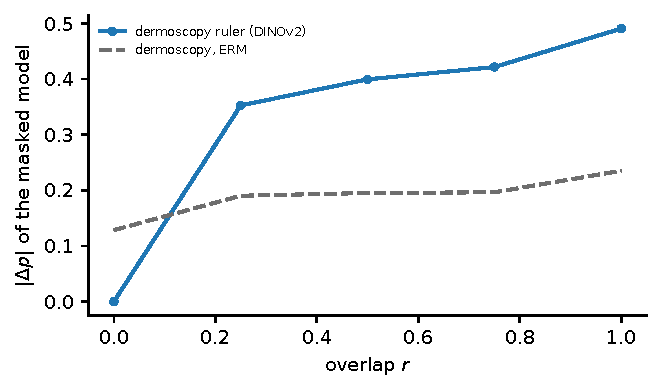
\includegraphics[width=0.66\linewidth]{../stage2_location_law_mechanism/figures/counterfactual.pdf}
\caption{Mean same-head sensitivity $|\Delta p|$ to inserting the artifact: masked model per sweep (solid) and ERM
for the dermoscopy sweep (dashed), by overlap.}\label{s2:fig:cf}\end{figure}

\paragraph{Lesion size} Table~\ref{s2:tab:tert}. The ruler covers a median \sTwoRatioLarge{} of a large lesion's area,
\sTwoRatioMedium{} of a medium and \sTwoRatioSmall{} of a small one. The harm at full overlap is significant for small
(\sTwoTertSmallOneZeroZero) and medium lesions (\sTwoTertMediumOneZeroZero) and not for large ones
(\sTwoTertLargeOneZeroZero, which \sTwoLargeVerdict); at 50\% overlap it is significant only for small lesions
(\sTwoTertSmallFiveZero; medium \sTwoTertMediumFiveZero). What holds is an ordering --- harm is largest where the
artifact is large relative to the lesion --- with wide intervals, because each tertile has few melanomas. No fixed ratio
threshold is claimed.
\begin{table}[H]\centering\scriptsize
\caption{Lesion-size strata of the controlled sweep (reversed-test AUROC, crossed CIs).}\label{s2:tab:tert}
\resizebox{\linewidth}{!}{\begin{tabular}{lccccc}\toprule
Lesion tertile & Ruler/lesion area (median) & Melanomas in test & mask $-$ ERM at 0\% & 50\% & 100\% \\\midrule
large & 0.012 & 36 & $+0.249$ [$+0.155, +0.346$] & $+0.087$ [$+0.006, +0.172$] & $+0.063$ [$-0.015, +0.144$] \\
medium & 0.031 & 21 & $+0.215$ [$+0.033, +0.391$] & $-0.129$ [$-0.283, +0.027$] & $-0.158$ [$-0.295, -0.027$] \\
small & 0.106 & 16 & $+0.150$ [$+0.036, +0.273$] & $-0.326$ [$-0.471, -0.176$] & $-0.364$ [$-0.509, -0.217$] \\
\bottomrule\end{tabular}}
\end{table}


\paragraph{Synthesis} Occlusion alone does not harm; restoring context does not remove the harm; harm follows whether
the artifact is visible after masking, and the masked model's reliance on a visible artifact is larger than ERM's.
The mechanism is \emph{retention with amplified reliance}: masking deletes the out-of-ROI evidence --- including other
cues that competed with the artifact --- and leaves the in-ROI artifact as a larger share of what predicts the label in
training, so the head weights it more heavily.

\subsubsection{Other modalities}
\begin{figure}[H]\centering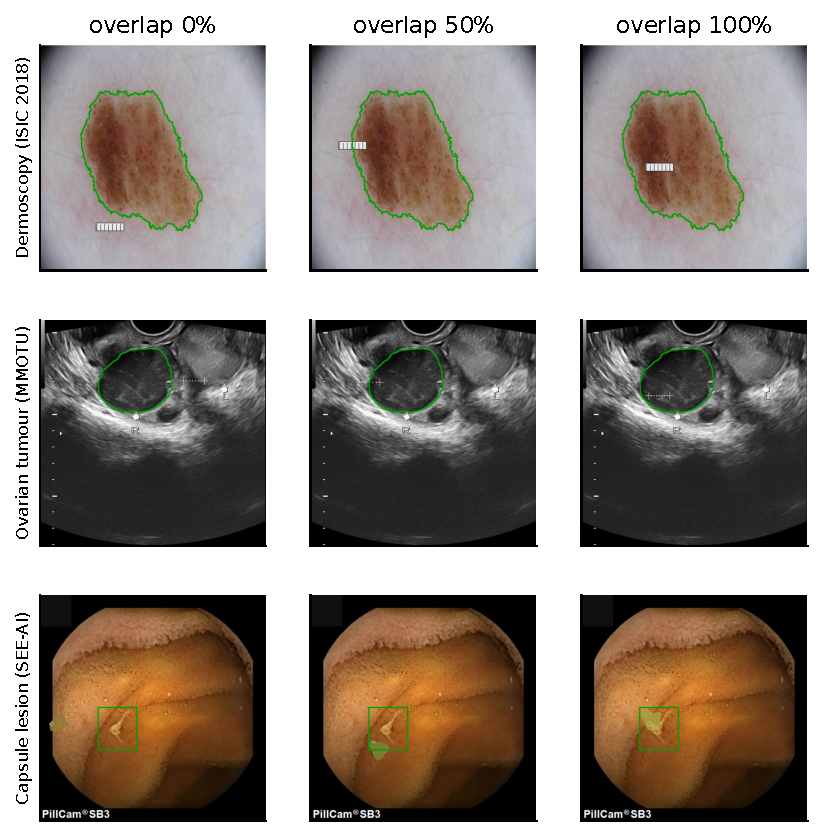
\includegraphics[width=0.86\linewidth]{../stage2_location_law_mechanism/figures/sweep_examples.pdf}
\caption{Real images with the synthetic artifact at 0, 50 and 100\% overlap (\textcolor{roigreen}{green}: ROI; the
capsule ROI is the annotated bounding box). Top: ISIC 2018 (CC BY-NC 4.0); middle: MMOTU ovarian ultrasound (CC BY
4.0); bottom: SEE-AI capsule endoscopy (CC BY 4.0). Thyroid (TN3K) and NIH images are not shown because their
redistribution terms are unclear.}\label{s2:fig:examples}\end{figure}
Table~\ref{s2:tab:other} and Figure~\ref{s2:fig:doseall} repeat the sweep in four further modalities; Table~\ref{s2:tab:otherarms}
gives every baseline arm. Across all \sTwoNSweeps{} controlled sweeps (four dermoscopy, seven others) the location
interaction is positive with an interval above zero in \sTwoNInterPos{} and negative in \sTwoNInterNeg. Whether the
falling benefit turns into harm at full overlap depends on the setting: masking harms significantly at full overlap in
\sTwoNHarmFull{} sweeps, still helps in \sTwoNHelpFull{} and makes no significant difference in \sTwoNNullFull.
\begin{table}[H]\centering\scriptsize
\caption{Controlled sweeps in the other modalities (synthetic caliper, debris, tube pasted at controlled overlap; reversed-test AUROC, crossed CIs).}\label{s2:tab:other}
\resizebox{\linewidth}{!}{\begin{tabular}{lccc}\toprule
Sweep & mask $-$ ERM at 0\% & at 100\% & Location interaction \\\midrule
Thyroid caliper, DINOv2 & $+0.402$ [$+0.315, +0.489$] & $-0.030$ [$-0.105, +0.042$] & $+0.433$ [$+0.362, +0.507$] \\
Thyroid caliper, MedSigLIP & $+0.514$ [$+0.430, +0.600$] & $+0.044$ [$-0.011, +0.104$] & $+0.470$ [$+0.388, +0.556$] \\
Ovarian caliper, DINOv2 & $+0.041$ [$-0.096, +0.175$] & $-0.197$ [$-0.357, -0.035$] & $+0.238$ [$+0.144, +0.340$] \\
Capsule debris, DINOv2 & $+0.116$ [$+0.052, +0.191$] & $-0.112$ [$-0.209, -0.019$] & $+0.228$ [$+0.144, +0.324$] \\
Capsule debris, MedSigLIP & $+0.374$ [$+0.248, +0.509$] & $+0.216$ [$+0.118, +0.317$] & $+0.158$ [$+0.012, +0.314$] \\
Chest tube, RAD-DINO & $-0.002$ [$-0.010, +0.005$] & $+0.111$ [$+0.095, +0.127$] & $-0.113$ [$-0.129, -0.097$] \\
Chest tube, DINOv2 & $+0.254$ [$+0.230, +0.278$] & $-0.083$ [$-0.112, -0.057$] & $+0.337$ [$+0.312, +0.364$] \\
\bottomrule\end{tabular}}
\end{table}

\begin{figure}[H]\centering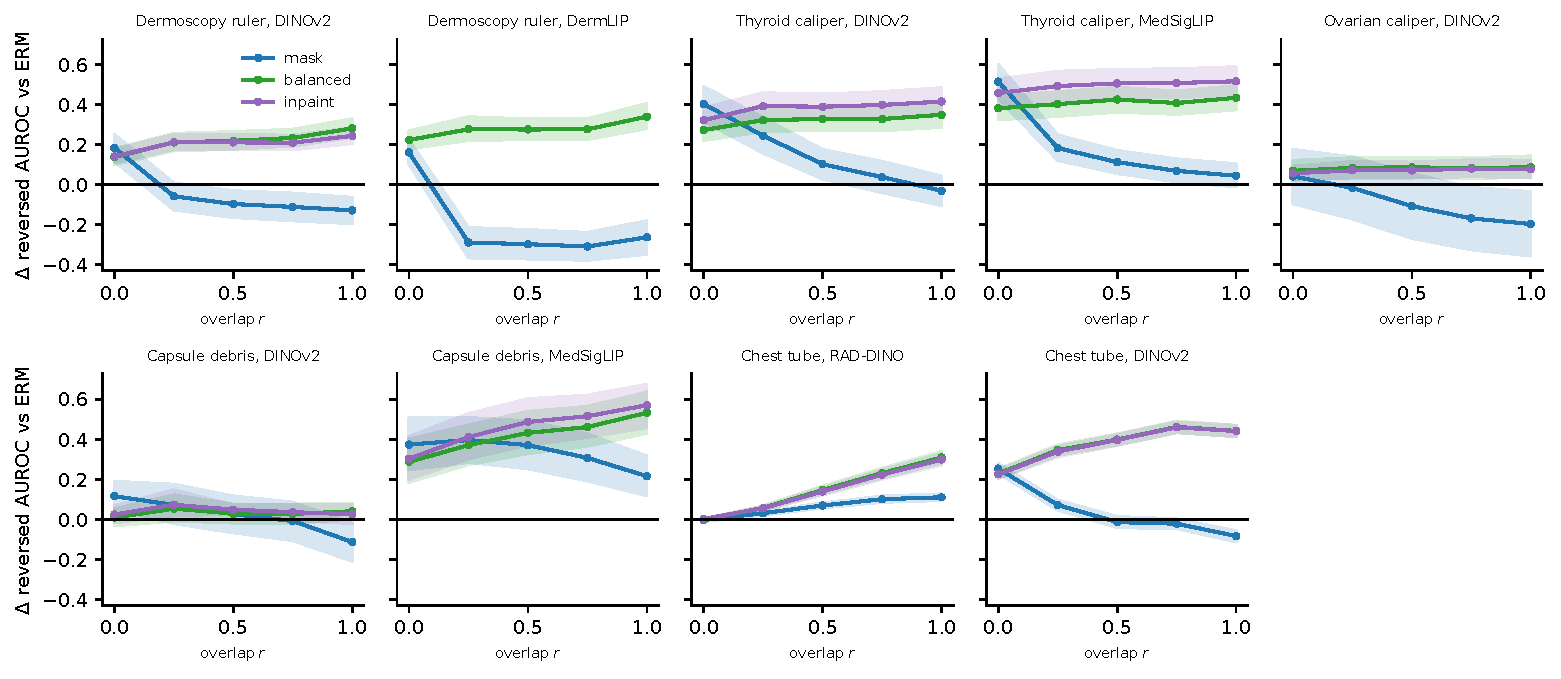
\includegraphics[width=\linewidth]{../stage2_location_law_mechanism/figures/dose_response_all.pdf}
\caption{Change in reversed-test AUROC versus ERM as a function of overlap, for masking (blue), group balancing (green)
and oracle inpainting (purple), in every controlled sweep (shaded: crossed 95\% CI). Masking falls with overlap in every
panel except the RAD-DINO chest tube.}\label{s2:fig:doseall}\end{figure}
\begin{itemize}[leftmargin=*]\itemsep1pt
\item \textbf{Thyroid calipers.} Masking helps strongly with the caliper outside the nodule (DINOv2
\sTwoThyroidcaliperDINOvTwoZero; MedSigLIP \sTwoThyroidcaliperMedSigLIPZero) and the benefit vanishes at full overlap
(\sTwoThyroidcaliperDINOvTwoFull; \sTwoThyroidcaliperMedSigLIPFull): the law holds as a loss of benefit, not as harm.
Nodules are large relative to the caliper, and the ultrasound background carries little disease information, so
masking costs little besides leaving the caliper.
\item \textbf{Ovarian calipers.} Masking harms at full overlap (\sTwoOvariancaliperDINOvTwoFull) and its benefit outside
the tumour is not significant (\sTwoOvariancaliperDINOvTwoZero): MMOTU tumours fill much of the frame, so little
background is removed, and the test set is small (64 images).
\item \textbf{Capsule debris.} With DINOv2 the sweep reverses (\sTwoCapsuledebrisDINOvTwoZero{} to
\sTwoCapsuledebrisDINOvTwoFull). With MedSigLIP masking still helps at full overlap (\sTwoCapsuledebrisMedSigLIPFull)
but less than outside (\sTwoCapsuledebrisMedSigLIPZero; interaction \sTwoCapsuledebrisMedSigLIPInter): the box ROI
contains much normal mucosa, so masking removes little of the lesion's context.
\item \textbf{Chest tube --- the boundary.} With RAD-DINO the ERM model ignores a tube outside the lungs (reversed
\sTwoCxrErmRevZero{} versus clean \sTwoCxrErmCleanZero{} at no overlap), so masking has nothing to remove at $r=0$; at
full overlap ERM collapses (\sTwoCxrErmRevOneZeroZero) and the masked model less so (\sTwoCxrMaskRevOneZeroZero). The
interaction is negative. With DINOv2, which does use the extra-pulmonary tube (reversed \sTwoCxrDinoErmRevZero{} versus
clean \sTwoCxrDinoErmCleanZero), the law holds (\sTwoChesttubeDINOvTwoInter). The law's premise is that the encoder
uses the out-of-ROI artifact; when it does not, masking cannot help outside and the law does not apply.
\item \textbf{The artifact-targeting arms} (inpainting, balancing, DFR, paired LEACE) help at both overlaps in every
modality except where the intervals are wide (ovary, DINOv2 capsule; Table~\ref{s2:tab:otherarms}). None of them shows the
positive location interaction of masking; most show a small negative one, because ERM relies more on an artifact that
sits on the lesion and there is more for them to remove.
\end{itemize}
{\scriptsize
\begin{longtable}{p{2.6cm}p{3.2cm}ccc}
\caption{All baseline arms in the controlled sweeps of the other modalities: ERM's clean and reversed AUROC and each arm's change in reversed-test AUROC versus ERM at no and at full overlap (crossed CIs). The last column is the arm's own location interaction ($[\cdot]_{r=0}-[\cdot]_{r=1}$); an arm that does not depend on where the artifact sits has an interaction near zero.}\label{s2:tab:otherarms}\\\toprule
Sweep & Arm & $r=0$ & $r=1$ & Location interaction \\\midrule
\endfirsthead
\toprule Sweep & Arm & $r=0$ & $r=1$ & Location interaction \\\midrule
\endhead
\bottomrule
\endlastfoot
Thyroid caliper, DINOv2 & ERM (AUROC: clean; reversed) & 0.666; 0.417 & 0.643; 0.325 & --- \\
 & masking $-$ ERM & $+0.402$ [$+0.315, +0.489$] & $-0.030$ [$-0.105, +0.042$] & $+0.433$ [$+0.362, +0.507$] \\
 & oracle inpainting $-$ ERM & $+0.321$ [$+0.261, +0.383$] & $+0.415$ [$+0.348, +0.484$] & $-0.093$ [$-0.124, -0.065$] \\
 & group-balanced $-$ ERM & $+0.273$ [$+0.220, +0.328$] & $+0.349$ [$+0.286, +0.415$] & $-0.076$ [$-0.106, -0.048$] \\
 & DFR $-$ ERM & $+0.299$ [$+0.228, +0.374$] & $+0.384$ [$+0.298, +0.472$] & $-0.085$ [$-0.123, -0.050$] \\
 & paired LEACE $-$ ERM & $+0.324$ [$+0.264, +0.386$] & $+0.420$ [$+0.353, +0.488$] & $-0.096$ [$-0.129, -0.066$] \\
Thyroid caliper, MedSigLIP & ERM (AUROC: clean; reversed) & 0.742; 0.320 & 0.723; 0.260 & --- \\
 & masking $-$ ERM & $+0.514$ [$+0.430, +0.600$] & $+0.044$ [$-0.011, +0.104$] & $+0.470$ [$+0.388, +0.556$] \\
 & oracle inpainting $-$ ERM & $+0.457$ [$+0.388, +0.527$] & $+0.516$ [$+0.442, +0.589$] & $-0.059$ [$-0.089, -0.031$] \\
 & group-balanced $-$ ERM & $+0.381$ [$+0.324, +0.442$] & $+0.433$ [$+0.373, +0.494$] & $-0.052$ [$-0.084, -0.020$] \\
 & DFR $-$ ERM & $+0.437$ [$+0.370, +0.505$] & $+0.484$ [$+0.409, +0.561$] & $-0.047$ [$-0.086, -0.008$] \\
 & paired LEACE $-$ ERM & $+0.460$ [$+0.389, +0.531$] & $+0.517$ [$+0.442, +0.587$] & $-0.057$ [$-0.089, -0.027$] \\
Ovarian caliper, DINOv2 & ERM (AUROC: clean; reversed) & 0.668; 0.656 & 0.677; 0.635 & --- \\
 & masking $-$ ERM & $+0.041$ [$-0.096, +0.175$] & $-0.197$ [$-0.357, -0.035$] & $+0.238$ [$+0.144, +0.340$] \\
 & oracle inpainting $-$ ERM & $+0.057$ [$+0.025, +0.092$] & $+0.077$ [$+0.034, +0.122$] & $-0.021$ [$-0.047, +0.004$] \\
 & group-balanced $-$ ERM & $+0.069$ [$+0.020, +0.121$] & $+0.087$ [$+0.034, +0.143$] & $-0.018$ [$-0.048, +0.009$] \\
 & DFR $-$ ERM & $+0.013$ [$-0.079, +0.102$] & $+0.047$ [$-0.049, +0.142$] & $-0.034$ [$-0.077, +0.005$] \\
 & paired LEACE $-$ ERM & $+0.056$ [$+0.023, +0.093$] & $+0.073$ [$+0.031, +0.119$] & $-0.017$ [$-0.044, +0.011$] \\
Capsule debris, DINOv2 & ERM (AUROC: clean; reversed) & 0.853; 0.822 & 0.849; 0.797 & --- \\
 & masking $-$ ERM & $+0.116$ [$+0.052, +0.191$] & $-0.112$ [$-0.209, -0.019$] & $+0.228$ [$+0.144, +0.324$] \\
 & oracle inpainting $-$ ERM & $+0.024$ [$-0.016, +0.069$] & $+0.026$ [$-0.020, +0.074$] & $-0.002$ [$-0.026, +0.024$] \\
 & group-balanced $-$ ERM & $+0.009$ [$-0.032, +0.053$] & $+0.041$ [$+0.004, +0.081$] & $-0.032$ [$-0.073, +0.001$] \\
 & DFR $-$ ERM & $+0.030$ [$-0.034, +0.090$] & $+0.049$ [$-0.016, +0.114$] & $-0.019$ [$-0.041, +0.001$] \\
 & paired LEACE $-$ ERM & $+0.035$ [$+0.014, +0.061$] & $+0.059$ [$+0.030, +0.094$] & $-0.023$ [$-0.043, -0.006$] \\
Capsule debris, MedSigLIP & ERM (AUROC: clean; reversed) & 0.902; 0.586 & 0.887; 0.302 & --- \\
 & masking $-$ ERM & $+0.374$ [$+0.248, +0.509$] & $+0.216$ [$+0.118, +0.317$] & $+0.158$ [$+0.012, +0.314$] \\
 & oracle inpainting $-$ ERM & $+0.303$ [$+0.201, +0.414$] & $+0.570$ [$+0.459, +0.675$] & $-0.267$ [$-0.388, -0.145$] \\
 & group-balanced $-$ ERM & $+0.288$ [$+0.185, +0.402$] & $+0.533$ [$+0.430, +0.636$] & $-0.245$ [$-0.359, -0.130$] \\
 & DFR $-$ ERM & $+0.294$ [$+0.186, +0.416$] & $+0.575$ [$+0.453, +0.695$] & $-0.281$ [$-0.398, -0.160$] \\
 & paired LEACE $-$ ERM & $+0.319$ [$+0.212, +0.433$] & $+0.608$ [$+0.499, +0.711$] & $-0.289$ [$-0.405, -0.171$] \\
Chest tube, RAD-DINO & ERM (AUROC: clean; reversed) & 0.915; 0.913 & 0.907; 0.614 & --- \\
 & masking $-$ ERM & $-0.002$ [$-0.010, +0.005$] & $+0.111$ [$+0.095, +0.127$] & $-0.113$ [$-0.129, -0.097$] \\
 & oracle inpainting $-$ ERM & $+0.003$ [$+0.002, +0.004$] & $+0.299$ [$+0.271, +0.329$] & $-0.297$ [$-0.326, -0.267$] \\
 & group-balanced $-$ ERM & $+0.000$ [$-0.004, +0.004$] & $+0.309$ [$+0.280, +0.339$] & $-0.309$ [$-0.338, -0.281$] \\
 & DFR $-$ ERM & $-0.014$ [$-0.022, -0.007$] & $+0.280$ [$+0.248, +0.313$] & $-0.294$ [$-0.328, -0.262$] \\
 & paired LEACE $-$ ERM & $+0.003$ [$+0.002, +0.004$] & $+0.287$ [$+0.259, +0.316$] & $-0.284$ [$-0.314, -0.255$] \\
Chest tube, DINOv2 & ERM (AUROC: clean; reversed) & 0.859; 0.629 & 0.852; 0.410 & --- \\
 & masking $-$ ERM & $+0.254$ [$+0.230, +0.278$] & $-0.083$ [$-0.112, -0.057$] & $+0.337$ [$+0.312, +0.364$] \\
 & oracle inpainting $-$ ERM & $+0.225$ [$+0.204, +0.247$] & $+0.442$ [$+0.413, +0.470$] & $-0.216$ [$-0.235, -0.198$] \\
 & group-balanced $-$ ERM & $+0.229$ [$+0.206, +0.251$] & $+0.442$ [$+0.414, +0.470$] & $-0.214$ [$-0.231, -0.196$] \\
 & DFR $-$ ERM & $+0.218$ [$+0.197, +0.240$] & $+0.433$ [$+0.406, +0.460$] & $-0.214$ [$-0.234, -0.196$] \\
 & paired LEACE $-$ ERM & $+0.233$ [$+0.212, +0.255$] & $+0.452$ [$+0.424, +0.481$] & $-0.219$ [$-0.238, -0.202$] \\
\end{longtable}}


\subsubsection{Sensitivity to the interval estimator}
As in Stage~1, both estimators were computed on the same predictions of the other-modality sweeps
(Table~\ref{s2:tab:estcheck}): the crossed intervals are wider by a median factor of \sTwoEstMed; \sTwoEstLost{} of
\sTwoEstN{} contrasts lose significance and none gains it (Table~\ref{s2:tab:estchanges}). Every statement in this stage
uses the crossed intervals, so these changes are already reflected in the text: in particular, MedSigLIP's small benefit
at full thyroid overlap and the ovarian harm at 50\% overlap are not claimed.
\begin{table}[H]\centering\scriptsize
\caption{The sweeps of the other modalities under the per-seed and the crossed estimator (same predictions; baseline arms only).}\label{s2:tab:estcheck}
\begin{tabular}{p{5.0cm}p{1.4cm}p{2.6cm}p{2.6cm}p{2.4cm}}\toprule
Result group & Intervals & Excluded 0 only with the per-seed estimator & Excluded 0 only with the crossed estimator & Median width ratio (crossed / per-seed) \\\midrule
synthetic/\allowbreak{}capsule & 60 & 9 & 0 & 1.72 \\
synthetic/\allowbreak{}nih\_ptx & 30 & 0 & 0 & 1.44 \\
synthetic/\allowbreak{}ovary & 30 & 1 & 0 & 1.59 \\
synthetic/\allowbreak{}thyroid & 60 & 1 & 0 & 1.37 \\
\textbf{all} & 180 & 11 & 0 & 1.45 \\
\bottomrule\end{tabular}
\end{table}

\begin{table}[H]\centering\scriptsize
\caption{Contrasts of the other-modality sweeps whose verdict depends on the estimator.}\label{s2:tab:estchanges}
\begin{tabular}{p{4.2cm}p{5.2cm}p{3.3cm}p{2.6cm}}\toprule
Result & Contrast & Crossed estimate [95\% CI] & Verdict vs per-seed estimator \\\midrule
synthetic/\allowbreak{}thyroid/\allowbreak{}medsiglip448\_caliper\_corr\_main & 1.0 /\allowbreak{} mask /\allowbreak{} erm /\allowbreak{} test\_rev & $+0.044$ [$-0.011, +0.104$] & no longer excludes 0 \\
synthetic/\allowbreak{}capsule/\allowbreak{}dino518\_debris\_corr\_main & 0.0 /\allowbreak{} inpaint /\allowbreak{} erm /\allowbreak{} test\_rev & $+0.024$ [$-0.016, +0.069$] & no longer excludes 0 \\
synthetic/\allowbreak{}capsule/\allowbreak{}dino518\_debris\_corr\_main & 0.75 /\allowbreak{} inpaint /\allowbreak{} erm /\allowbreak{} test\_rev & $+0.036$ [$-0.005, +0.074$] & no longer excludes 0 \\
synthetic/\allowbreak{}capsule/\allowbreak{}dino518\_debris\_corr\_main & 1.0 /\allowbreak{} inpaint /\allowbreak{} erm /\allowbreak{} test\_rev & $+0.026$ [$-0.020, +0.074$] & no longer excludes 0 \\
synthetic/\allowbreak{}capsule/\allowbreak{}dino518\_debris\_corr\_main & 0.5 /\allowbreak{} balanced /\allowbreak{} erm /\allowbreak{} test\_rev & $+0.030$ [$-0.018, +0.076$] & no longer excludes 0 \\
synthetic/\allowbreak{}capsule/\allowbreak{}dino518\_debris\_corr\_main & 0.75 /\allowbreak{} balanced /\allowbreak{} erm /\allowbreak{} test\_rev & $+0.028$ [$-0.023, +0.076$] & no longer excludes 0 \\
synthetic/\allowbreak{}capsule/\allowbreak{}dino518\_debris\_corr\_main & 0.0 /\allowbreak{} dfr /\allowbreak{} erm /\allowbreak{} test\_rev & $+0.030$ [$-0.034, +0.090$] & no longer excludes 0 \\
synthetic/\allowbreak{}capsule/\allowbreak{}dino518\_debris\_corr\_main & 0.5 /\allowbreak{} dfr /\allowbreak{} erm /\allowbreak{} test\_rev & $+0.048$ [$-0.014, +0.110$] & no longer excludes 0 \\
synthetic/\allowbreak{}capsule/\allowbreak{}dino518\_debris\_corr\_main & 0.75 /\allowbreak{} dfr /\allowbreak{} erm /\allowbreak{} test\_rev & $+0.055$ [$-0.010, +0.122$] & no longer excludes 0 \\
synthetic/\allowbreak{}capsule/\allowbreak{}dino518\_debris\_corr\_main & 1.0 /\allowbreak{} dfr /\allowbreak{} erm /\allowbreak{} test\_rev & $+0.049$ [$-0.016, +0.114$] & no longer excludes 0 \\
synthetic/\allowbreak{}ovary/\allowbreak{}dino518\_caliper\_corr\_main & 0.5 /\allowbreak{} mask /\allowbreak{} erm /\allowbreak{} test\_rev & $-0.107$ [$-0.269, +0.054$] & no longer excludes 0 \\
\bottomrule\end{tabular}
\end{table}


\subsection{What failed or changed}\label{s2:sec:changed}
\begin{itemize}[leftmargin=*]\itemsep1pt
\item \textbf{Harm at full overlap is not universal.} The robust statement is the \emph{interaction} (\sTwoNInterPos{}
of \sTwoNSweeps); harm at full overlap is significant in \sTwoNHarmFull{} of \sTwoNSweeps{} sweeps.
\item \textbf{Two lesion-size cells are not significant} (large lesions at full overlap, medium lesions at 50\%): harm
is ordered by lesion size, not monotone in every cell.
\item \textbf{Chest radiography with RAD-DINO contradicts the law}, as a failure of its premise. It was registered as a
confirmation and is reported as a boundary case.
\item \textbf{The counterfactual mechanism holds in \sTwoCfNPos{} of \sTwoCfN{} sweeps}: not for thyroid calipers (equal
sensitivity) and reversed for the chest tube with RAD-DINO.
\item \textbf{The ovarian sweep has no significant benefit outside the ROI}, so its interaction rests on the harm side.
\item \textbf{Reproducibility of the capsule split.} The capsule sweep's split is produced by a seeded shuffle of the
group list; rebuilding the cohort (a re-derived contamination mask moved a few frames across the 5\% threshold) re-dealt
the split, and only 32 of 71 artifact-bearing test frames of an earlier build recur. Point estimates of that sweep moved
by up to about 0.2, while the location interaction kept its sign and significance. The split is now frozen with the
cohort file.
\end{itemize}

\subsection{Anticipated questions}
\paragraph{Why not simply show saliency maps?} They show where a model looks, not how much its decision depends on the
artifact, and they are unstable for frozen encoders with linear heads. The same-head counterfactual answers the causal
question directly on the same image.
\paragraph{If masking removes context, why is the occlusion control not harmed?} Because in the occlusion control the
ruler is uninformative: the head does not need it, so keeping it costs nothing, and the context lost by masking is
small for this task. The harm in the sweep appears only when the retained ruler predicts the label in training.
\paragraph{Why does dilation make things worse at 50\% overlap?} Because it makes more of the ruler visible (retention
0.50 $\to$ 0.95) while adding only a thin rim of context. The shortcut becomes stronger; the head uses it more.
\paragraph{Why does the harm not grow at 100\% overlap when the mask is dilated?} The ruler is already fully visible;
dilation only adds skin. If harm were about the ruler's share of the image it would fall; it does not.
\paragraph{Why do the artifact-targeting arms help \emph{more} when the artifact is inside?} ERM relies more on a ruler
on the lesion (its reversed AUROC is lower at $r=1$), so removing that reliance gains more. Their gain does not depend
on the ROI.
\paragraph{Why does thyroid show loss of benefit rather than harm?} The ultrasound background contains little disease
information, so masking loses almost nothing besides failing to remove the caliper; ERM is already caliper-driven, and
masking leaves it so. Harm needs masking to remove disease evidence as well.
\paragraph{Why is the chest tube a boundary and not a failure?} The law compares what masking removes outside and
inside the ROI. RAD-DINO does not use the out-of-lung tube at all (reversed $\approx$ clean AUROC), so there is nothing to
remove outside and the comparison has no content. DINOv2 uses the tube and shows the law.
\paragraph{Are 3 seeds enough?} For the interactions, yes: the intervals include the variation of the fixed test set,
and \sTwoNInterPos{} of \sTwoNSweeps{} exclude zero. Individual cells in small cohorts (ovary) are imprecise and are
interpreted only through the interaction.
\paragraph{Could the synthetic artifacts be unrealistic?} Yes, and that is their purpose: they isolate location.
Whether the law holds for artifacts that clinicians actually produce is a separate question that synthetic sweeps
cannot answer.

\subsection{Conclusion}
\textbf{Supported.} The location law in its interaction form (Q2a) holds in \sTwoNInterPos{} of \sTwoNSweeps{}
controlled sweeps across five modalities and four encoders. The mechanism (Q2b) is retention with amplified reliance:
occlusion alone does not harm, harm follows the visibility of the artifact under dilation, and the masked head's
same-image reliance on an in-ROI artifact is about \sTwoDpRatioFull{} times that of ERM for the ruler (\sTwoDpDiffFull)
and significantly higher in \sTwoCfNPos{} of \sTwoCfN{} sweeps. \textbf{Qualified.} Harm at full overlap is
setting-dependent; the lesion-size gradient is an ordering. \textbf{Not supported.} The law for an encoder that ignores
the out-of-ROI artifact (chest tube, RAD-DINO). The practical reading is: masking removes what lies outside the ROI and
concentrates the model on what lies inside; whether that helps depends on where the shortcut sits.

\subsection{Questions for the supervisor}
\begin{enumerate}\itemsep1pt
\item Should the thesis state the law in its interaction form only (robust) and treat harm at full overlap as
setting-dependent, or keep harm as the headline for dermoscopy, where it holds with every encoder?
\item The counterfactual mechanism holds in \sTwoCfNPos{} of \sTwoCfN{} sweeps. Is the thyroid result (the unmasked model
is already as reliant on an in-nodule caliper as the masked one) best presented as a limitation or as a second route to
the same outcome?
\item Is it acceptable to present chest radiography with RAD-DINO as a boundary of the law rather than as a failed
confirmation, given that it was registered as a confirmation?
\end{enumerate}


\clearpage
% generated by make_combined.py from stage3_real_artifacts/stage3.tex; do not edit
\section{Stage 3 --- Real artifacts across modalities}\label{sec:stage3}

\stagebox{\textbf{In one sentence.} With real, unedited artifacts --- hair in dermoscopy, calipers in thyroid and
ovarian ultrasound, debris in capsule endoscopy --- ROI masking helps far more when the artifact lies outside the ROI
than inside it: the crossover is positive in \sThreeNXPos{} of \sThreeNRuns{} cohort--encoder pairs and in all four
pre-specified location tests after Holm correction; the dermatology encoder DermLIP and, with the radiograph encoder
RAD-DINO, real chest-radiograph devices are the exceptions, and the hair shortcut turns out to be carried largely by correlates of hair rather than by its
pixels.}
\subsection{Where this stage starts}
Stage~1 showed with real hair (E13) that masking harms when hair lies on the lesion and helps when it lies beside it.
Stage~2 established the location law with synthetic artifacts whose position was controlled, in five modalities, and
identified its mechanism (retention with amplified reliance). Synthetic artifacts answer \emph{whether} location can
matter; they cannot show that it matters for the artifacts clinicians actually produce, whose location is set by the
workflow and read from masks. This stage builds real-artifact traps in three more cohorts, validates the automatic
artifact masks that define ``inside'' and ``outside'', replicates across encoder families, asks what actually carries
the hair shortcut, and examines chest radiography, where the law might not hold.

\subsection{Questions}
\begin{enumerate}[label=\textbf{Q3\alph*},leftmargin=*]\itemsep1pt
\item With real artifacts and the same protocol, is ROI masking less useful --- or harmful --- when the artifact lies
inside the ROI than when it lies outside it (a positive crossover)?
\item Does this hold across modalities, artifacts and encoder families?
\item Are the artifact masks that define inside and outside good enough to support the answer?
\item What carries a real shortcut: the artifact's pixels, or things that go with the artifact?
\end{enumerate}
\paragraph{Design: two traps sharing one artifact-free group} A real artifact's location is fixed by the image, so it
cannot be moved. Each cohort is split into images whose artifact lies mostly inside the ROI ($r\ge0.5$, Trap~A) and
images whose artifact lies outside it ($r<0.1$, Trap~B); images with $0.1\le r<0.5$ belong to neither trap. Each trap is
completed by the \emph{same} artifact-free images and receives the environments of Stage~1. This is the E13 design of
Stage~1, which replaced the pilot's overlap-contrast design (E12) because in E12 location itself was the label proxy.
\paragraph{Why these cohorts} Each has (i) an artifact that clinicians produce and that is associated with the
diagnosis through the workflow (calipers are placed on nodules that are measured; debris is more frequent on some lesion
types), (ii) public ROI masks or boxes, (iii) a way to locate the artifact without manual annotation, and (iv) enough
images for an artifact-free group. Table~\ref{s3:tab:rejected} lists the cohorts that failed one of these conditions.

\subsection{Methods}
\subsubsection{Cohorts}
\begin{itemize}[leftmargin=*]\itemsep1pt
\item \textbf{Dermoscopy} --- ISIC 2019 \citep{combalia2019bcn,tschandl2018ham} as in Stage~1: published semi-automatic
hair masks \citep{wegley2026artifacts}; lesion masks from HAM10000 or the U-Net trained on ISIC 2018 Task~1
\citep{codella2019isic}; leakage groups lesion identifier $\cup$ perceptual hash.
\item \textbf{Thyroid ultrasound} --- TN3K images \citep{gong2021tn3k} with TNCD benign/malignant labels (3,493
images, 1,210 malignant) and manual nodule masks. Calipers located by a rule-based detector (dotted measurement lines =
$\ge7$ evenly spaced bright dots; ``+'' calipers by template matching), tuned on 36 images and frozen before its final
audit. $A=0$: no detected caliper pixel; $A=1$: $\ge15$ detected pixels. Groups: pHash $\le8$ (TN3K publishes no
patient identifiers).
\item \textbf{Ovarian ultrasound} --- MMOTU OTU\_2d \citep{zhao2022mmotu} (CC BY 4.0): benign cystic lesions (chocolate
cyst, serous cystadenoma, simple cyst) versus lesions with a solid component (teratoma, theca cell tumour, mucinous
cystadenoma, high-grade serous carcinoma); normal ovaries excluded (1,202 images). The frozen thyroid detector,
unchanged. Groups: pHash $\le8$.
\item \textbf{Capsule endoscopy} --- SEE-AI \citep{seeai2023} (CC BY 4.0), single-class frames: erosion versus
polyp-like lesions; ROI = union of the expert lesion boxes. Contamination (debris, bubbles, bile) masks from the
published expert masks where available (22 frames) and otherwise from a linear probe on DINOv2 patch tokens trained on
2,160 expert-masked frames. $A=0$: contamination $<3\%$ of the frame; $A=1$: $\ge10\%$. Groups: blocks of 100
consecutive frame numbers $\cup$ pHash $\le2$ (no video identifiers are published).
\item \textbf{Chest radiography} --- NIH ChestX-ray14 \citep{wang2017chestxray8}; lungs from a PSPNet
\citep{cohen2022xrv}. (i) \emph{Device traps}: images linked to RANZCR-CLiP device annotations; Trap~A = central venous
catheter inside the lungs, Trap~B = endotracheal tube outside them; four findings with $\ge40$ reversed-test positives;
restricted to AP films (intubated patients are imaged supine, so view could not be matched). (ii) \emph{Chest drains}:
29,687 pneumothorax-labelled images; drains from NEATX human labels and a drain detector (precision 0.95); drains lie
inside the lungs, so this is an in-ROI trap only. Patient-grouped folds.
\end{itemize}
\paragraph{Protocol} Frozen encoders: DINOv2 ViT-B/14 @518 for every cohort; MedSigLIP-448 (a medical vision--language
model) for thyroid, ovary and capsule; ConvNeXt-Base @384 (a CNN) for thyroid and capsule; DermLIP for dermoscopy;
RAD-DINO for chest radiographs. Logistic heads chosen on clean validation data; 5 seeds (42, 123, 456, 789, 2026)
$\times$ 5 grouped folds, fold predictions pooled per seed. Within each label the artifact-bearing images are
subsampled to the source mix of the artifact-free group (source matching; vacuous for single-source cohorts). Gates
fixed before fitting: every matched cell $\ge25$ images and $\ge40$ reversed-test positives. Arms as in Stage~1.
\paragraph{Statistics} Crossed seed$\times$image bootstrap, 10,000 replicates; the crossover's interval resamples the
same images in both traps. The four location tests (P1, one per cohort, DINOv2) are Holm-corrected; everything else is
reported with unadjusted 95\% intervals.

\subsection{Experiments}
\begin{table}[H]\centering\scriptsize
\caption{Experiments of this stage with registration status, the registration document (\texttt{docs/PREREGISTRATION\_<name>.md}), its first commit and the support criterion stated in advance. Commit times are set by the committing machine and are not independent proof of order.}\label{s3:tab:exp}
\begin{tabular}{p{3.1cm}p{2.1cm}p{2.4cm}p{3.2cm}p{3.3cm}}\toprule
Experiment & Status & Registration & First commit (local time) & Support criterion \\\midrule
Dermoscopy hair traps (E13, DINOv2) & \ok{} registered & ISIC2019\_\allowbreak{}TRAPS & \texttt{76e25d4}, 2026-09-26 13:14 & crossover CI $>0$ \\
Dermoscopy hair, DermLIP & \ok{} registered & ISIC2019\_\allowbreak{}TRAPS & \texttt{76e25d4}, 2026-09-26 13:14 & crossover CI $>0$ \\
Thyroid caliper traps & \ok{} registered & THYROID\_\allowbreak{}TRAPS & \texttt{ea57661}, 2026-09-26 22:46 & crossover CI $>0$ \\
Ovarian caliper traps & \ok{} registered & OVARY\_\allowbreak{}TRAPS & \texttt{2517600}, 2026-09-27 07:29 & crossover CI $>0$ \\
Capsule debris traps & \ok{} registered & CAPSULE\_\allowbreak{}TRAPS & \texttt{fcbf8d9}, 2026-09-27 00:40 & crossover CI $>0$ \\
Chest-radiograph device traps & \ok{} registered & CXR\_\allowbreak{}DEVICE\_\allowbreak{}TRAPS & \texttt{4d1a924}, 2026-09-26 18:07 & crossover CI $>0$ \\
Location tests P1 (four cohorts, Holm) & \mixed{} each test registered; Holm grouping post hoc & STATISTICAL\_\allowbreak{}PLAN & \texttt{4e9d44c}, 2026-09-27 09:37 & Holm $p<0.05$, positive estimate \\
Chest drains (NIH) & \ok{} registered & CXR\_\allowbreak{}DRAIN & \texttt{3d0cffc}, 2026-09-27 03:29 & mask $-$ ERM reported with CI, no direction \\
Crossed-bootstrap intervals (A1) & \ok{} registered & FINAL (A1) & \texttt{c45d482}, 2026-09-28 00:35 & a claim is stated only if its crossed CI excludes 0 \\
\bottomrule\end{tabular}
\end{table}


\subsection{Results}
\subsubsection{Cohorts and artifact masks}
\begin{table}[H]\centering\scriptsize
\caption{Real-artifact cohorts and pool sizes (images, positive/negative diagnosis) before the environments are sampled. Trap A: artifact mostly inside the ROI ($r\ge0.5$); Trap B: outside ($r<0.1$); both share the artifact-free group.}\label{s3:tab:cohorts}
\resizebox{\linewidth}{!}{\begin{tabular}{p{3.4cm}p{2.4cm}p{2.5cm}p{2.2cm}ccc}\toprule
Cohort & Task & Artifact (mask source) & ROI & Artifact-free pos/neg & Trap A pos/neg & Trap B pos/neg \\\midrule
ISIC 2019 dermoscopy (HAM10000, BCN20000, MSK) & melanoma vs other & hair (published masks) & lesion: HAM manual / U-Net & 157/706 & 942/2655 & 969/4412 \\
TN3K ultrasound, TNCD labels & malignant vs benign nodule & calipers (rule detector) & nodule (manual) & 749/1052 & 292/858 & 99/227 \\
MMOTU 2D ultrasound & solid-component vs cystic tumour & calipers (rule detector) & tumour (manual) & 178/170 & 276/341 & 103/91 \\
SEE-AI capsule endoscopy & erosion vs polyp-like lesion & debris (patch probe) & lesion box (expert) & 343/164 & 412/404 & 1009/231 \\
\bottomrule\end{tabular}}
\end{table}

\begin{figure}[H]\centering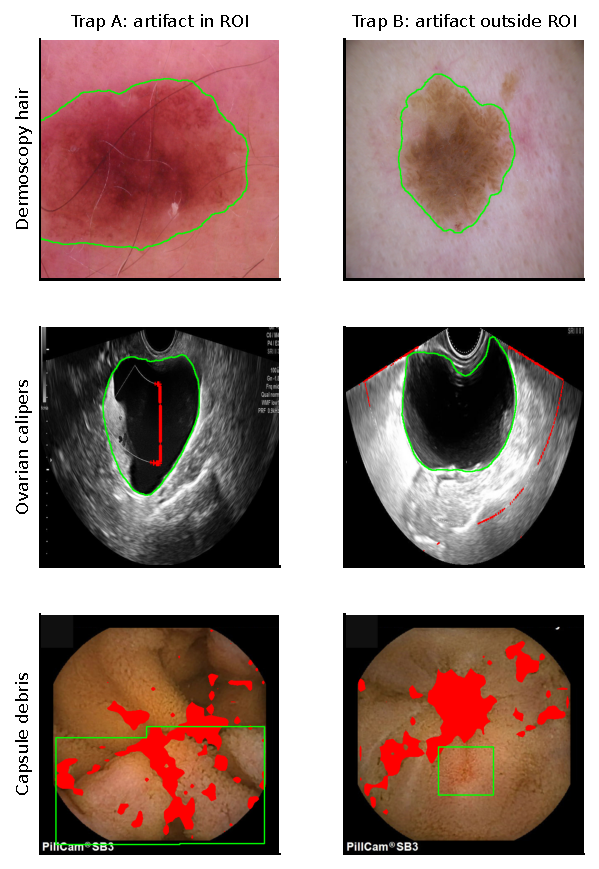
\includegraphics[width=0.60\linewidth]{../stage3_real_artifacts/figures/real_examples.pdf}
\caption{Real artifacts inside (Trap~A) and outside (Trap~B) the ROI. \textcolor{roigreen}{Green}: ROI;
\textcolor{artred}{red}: automatic artifact mask. Dermoscopy is shown with the lesion outline only (the published hair
masks carry no redistribution licence). Thyroid images are not shown (data licence not stated). Automatic overlap of
the shown images: dermoscopy \sThreeExRisichairinroi{} and \sThreeExRisichairoutroi; ovary \sThreeExRovarycalipersinroi{}
and \sThreeExRovarycalipersoutroi; capsule \sThreeExRcapsuledebrisinroi{} and \sThreeExRcapsuledebrisoutroi. ISIC CC
BY-NC 4.0; MMOTU, SEE-AI CC BY 4.0.}\label{s3:fig:ex}\end{figure}
\begin{figure}[H]\centering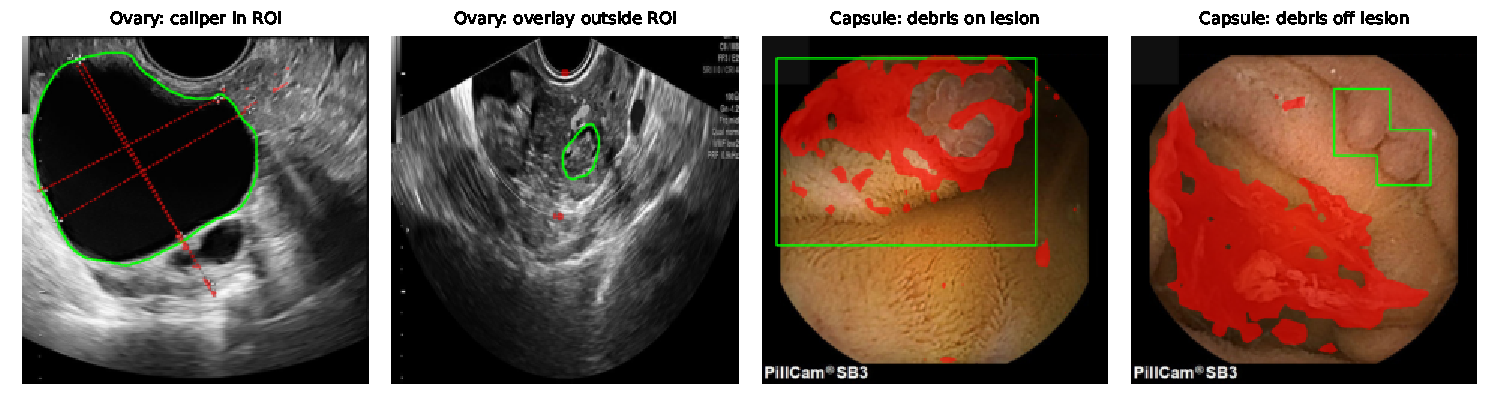
\includegraphics[width=\linewidth]{../../paper/figures/examples.pdf}
\caption{Further real examples with the automatic masks: ovarian calipers crossing the tumour and an overlay outside
it; capsule debris on and off the lesion boxes (MMOTU, SEE-AI; CC BY 4.0).}\label{s3:fig:ex2}\end{figure}
\paragraph{Mask validity} Table~\ref{s3:tab:det}. Lesion masks are accurate (U-Net held-out Dice \sThreeUnetDice; against
HAM manual masks \sThreeUnetHam). The capsule probe reaches pixel accuracy \sThreeProbeAcc{} and IoU \sThreeProbeIoU{}
against held-out expert masks. The thyroid detector's detections lie on a real caliper in 38 of 40 audited images, and
38--39 of 40 caliper-free images are clean. For the ovary, every detection is an on-screen overlay but only 31 of 40
are calipers (the others are dotted zoom arcs and focus markers), and the ``marker-free'' group is caliper-free but not
overlay-free. The morphological hair detector of the pilot is poor (IoU \sThreeHairDetIoU), which is why the hair traps
use the published masks.
\paragraph{Why label noise cannot create the result} An image mislabelled as artifact-bearing (or artifact-free)
weakens the constructed association between $A$ and $Y$ equally in both traps; it biases every effect toward zero. To
create a crossover, errors would have to depend on location \emph{and} on the label, which none of the detectors uses.
\begin{table}[H]\centering\scriptsize
\caption{Validity of the automatic masks that define artifact presence and location. Visual audits: \texttt{docs/ARTIFACT\_MASK\_AUDIT.md} and \texttt{docs/THYROID\_MARKER\_AUDIT.md} (visual audits during the analysis, not by a clinician).}\label{s3:tab:det}
\begin{tabular}{p{3.0cm}p{3.0cm}p{3.8cm}p{4.6cm}}\toprule
Mask & Source & Check & Result \\\midrule
ISIC 2019 lesion masks (BCN, MSK) & U-Net trained on ISIC 2018 Task 1 & held-out Dice (mean) / Dice vs HAM manual masks & 0.886 / 0.895 \\
Hair (DullRazor-type detector, E10) & morphological & IoU / precision / recall vs Mendeley masks & 0.222 / 0.316 / 0.472 \\
Capsule debris masks & patch-token probe (2,160 expert-masked frames) & held-out pixel accuracy / IoU & 0.922 / 0.625 \\
Thyroid (TN3K), detected (A1) & visual audit, 40 images & detection lies on a real caliper / measurement mark & 38/40 (95 \%); 2 border false positives; 1 dotted zoom box (overlay) \\
Thyroid, marker-free (A0) & visual audit, 40 images & no visible caliper & 38–39/40 (95–97 \%); depth-scale ticks present in all images (not label-related) \\
Ovary (MMOTU), detected (A1) & visual audit, 40 images & an on-screen overlay is present & 40/40; caliper specifically 31/40 (others: dotted zoom arcs, focus markers, thumbnail inset) \\
Ovary, marker-free (A0) & visual audit, 40 images & no visible caliper & 37/40 (92 \%) \\
Ovary, marker-free (A0) & visual audit, 40 images & no overlay of any kind (arrows, boxes) & $\sim$29/40 (72 \%); text labels common \\
\bottomrule\end{tabular}
\end{table}


\subsubsection{The crossover with real artifacts}
Table~\ref{s3:tab:traps} and Figure~\ref{s3:fig:forest}. With DINOv2, masking is worth less for in-ROI artifacts in every
cohort:
\begin{itemize}[leftmargin=*]\itemsep1pt
\item \textbf{Dermoscopy hair.} Masking \emph{harms} when the hair lies on the lesion (\sThreeAisicDINOvTwo) and helps
when it lies outside (\sThreeBisicDINOvTwo); crossover \sThreeXisicDINOvTwo{} (as in Stage~1). After masking the Trap-A
model still separates the correlated test (\sThreeMaskCorrAisicDINOvTwo) far better than the reversed one
(\sThreeMaskRevAisicDINOvTwo).
\item \textbf{Thyroid calipers.} Masking helps in both traps but far more when the calipers lie outside the nodule
(\sThreeBthyroidDINOvTwo{} versus \sThreeAthyroidDINOvTwo; crossover \sThreeXthyroidDINOvTwo). In Trap~A the masked model
remains caliper-driven: correlated \sThreeAucThyroidtrapAmaskCorr, reversed \sThreeAucThyroidtrapAmaskRev{}
(Table~\ref{s3:tab:aucenv}); in Trap~B masking removes the gap (\sThreeAucThyroidtrapBmaskCorr{} versus
\sThreeAucThyroidtrapBmaskRev).
\item \textbf{Ovarian calipers.} Crossover \sThreeXovaryDINOvTwo{} (Trap~A \sThreeAovaryDINOvTwo, Trap~B
\sThreeBovaryDINOvTwo).
\item \textbf{Capsule debris.} The largest crossover (\sThreeXcapsuleDINOvTwo): masking recovers almost all of the
reversed-test loss when the debris lies outside the lesion boxes (\sThreeBcapsuleDINOvTwo) and little when it lies on
them (\sThreeAcapsuleDINOvTwo).
\end{itemize}
\paragraph{Other encoder families} The crossover replicates with MedSigLIP (thyroid \sThreeXthyroidMedSigLIP, ovary
\sThreeXovaryMedSigLIP, capsule \sThreeXcapsuleMedSigLIP) and with the CNN ConvNeXt (thyroid \sThreeXthyroidConvNeXt,
capsule \sThreeXcapsuleConvNeXt). With ConvNeXt, masking is useless inside the nodule (\sThreeAthyroidConvNeXt) and
strongly helpful outside it (\sThreeBthyroidConvNeXt). The effect is not a property of vision transformers or of
self-supervised training.
\paragraph{Harm or loss of benefit?} Only for dermoscopy hair does masking actually harm in Trap~A. For calipers and
debris it still helps a little in Trap~A --- it removes clutter and overlays elsewhere on the screen --- but a large
residual shortcut remains. The universal real-data statement is therefore the \emph{crossover}; harm appears where
masking also removes disease context (dermoscopy, and in Stage~2 the controlled sweeps).
\begin{table}[H]\centering\scriptsize
\caption{Real-artifact traps: change in reversed-test AUROC from ROI masking, per trap, and the crossover (5 seeds $\times$ 5 grouped folds; crossed 95\% CIs).}\label{s3:tab:traps}
\resizebox{\linewidth}{!}{\begin{tabular}{lccccc}\toprule
Cohort & Encoder & ERM reversed AUROC A / B & mask $-$ ERM, Trap A (in ROI) & mask $-$ ERM, Trap B (outside) & Crossover B $-$ A \\\midrule
Dermoscopy hair & DINOv2 & 0.510 / 0.510 & $-0.049$ [$-0.083, -0.018$] & $+0.098$ [$+0.060, +0.136$] & $+0.147$ [$+0.111, +0.185$] \\
Dermoscopy hair & DermLIP & 0.665 / 0.735 & $-0.104$ [$-0.143, -0.067$] & $-0.090$ [$-0.135, -0.046$] & $+0.014$ [$-0.037, +0.063$] \\
Thyroid calipers & DINOv2 & 0.289 / 0.405 & $+0.109$ [$+0.085, +0.133$] & $+0.348$ [$+0.307, +0.388$] & $+0.239$ [$+0.196, +0.280$] \\
Thyroid calipers & MedSigLIP & 0.289 / 0.481 & $+0.053$ [$+0.032, +0.073$] & $+0.248$ [$+0.200, +0.293$] & $+0.195$ [$+0.153, +0.238$] \\
Ovarian calipers & DINOv2 & 0.413 / 0.423 & $+0.132$ [$+0.072, +0.196$] & $+0.302$ [$+0.225, +0.378$] & $+0.170$ [$+0.087, +0.252$] \\
Capsule debris & DINOv2 & 0.581 / 0.429 & $+0.084$ [$+0.055, +0.112$] & $+0.461$ [$+0.415, +0.506$] & $+0.377$ [$+0.327, +0.426$] \\
Capsule debris & MedSigLIP & 0.570 / 0.464 & $+0.117$ [$+0.088, +0.147$] & $+0.452$ [$+0.407, +0.495$] & $+0.335$ [$+0.286, +0.383$] \\
Thyroid calipers & ConvNeXt & 0.357 / 0.429 & $-0.004$ [$-0.029, +0.020$] & $+0.271$ [$+0.228, +0.314$] & $+0.275$ [$+0.231, +0.320$] \\
Ovarian calipers & MedSigLIP & 0.426 / 0.551 & $+0.002$ [$-0.048, +0.051$] & $+0.180$ [$+0.120, +0.238$] & $+0.178$ [$+0.109, +0.248$] \\
Capsule debris & ConvNeXt & 0.528 / 0.431 & $+0.084$ [$+0.049, +0.118$] & $+0.403$ [$+0.358, +0.448$] & $+0.320$ [$+0.268, +0.372$] \\
\bottomrule\end{tabular}}
\end{table}

\begin{figure}[H]\centering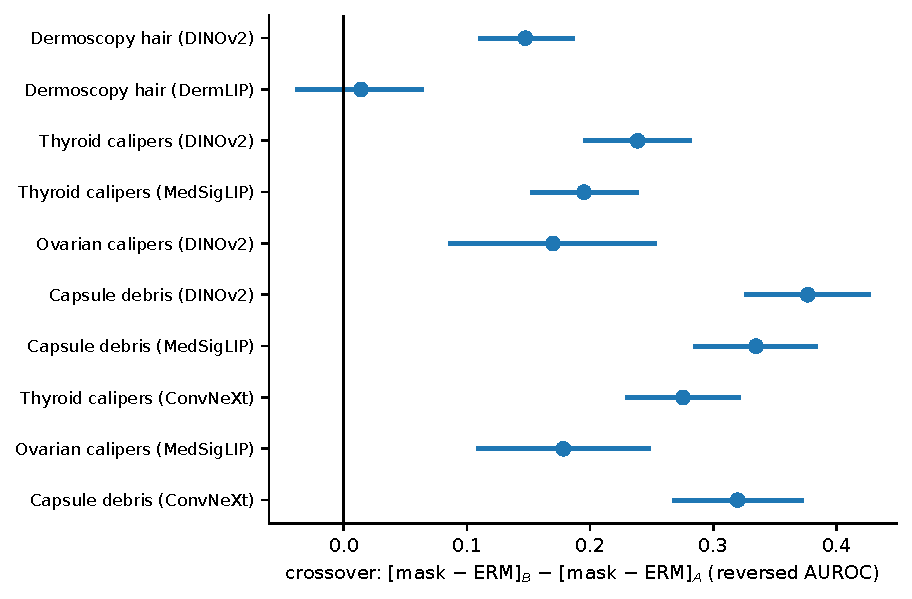
\includegraphics[width=0.78\linewidth]{../stage3_real_artifacts/figures/crossover_forest.pdf}
\caption{Crossover with real artifacts, per cohort and encoder (crossed 95\% CIs).}\label{s3:fig:forest}\end{figure}

\subsubsection{The four location tests}
Table~\ref{s3:tab:primary}. Each cohort's crossover test was registered with the cohort; they are grouped here into one
Holm family. All \sThreeNPOneOK{} of \sThreeNPOne{} are supported ($p\le$ \sThreePMax{} before adjustment).
\begin{table}[H]\centering\small
\caption{The four pre-specified location tests (P1: crossover $>0$), crossed bootstrap, two-sided bootstrap $p$ (floored at $10^{-4}$), Holm-adjusted over the four cohorts.}\label{s3:tab:primary}
\begin{tabular}{lcccc}\toprule
Cohort (DINOv2) & Crossover [95\% CI] & $p$ & $p$ (Holm, 4) & Supported \\\midrule
ISIC hair (DINOv2) & $+0.147$ [$+0.111, +0.185$] & 0.0001 & 0.0004 & \ok \\
Thyroid (DINOv2) & $+0.239$ [$+0.196, +0.280$] & 0.0001 & 0.0004 & \ok \\
Capsule (DINOv2) & $+0.377$ [$+0.327, +0.426$] & 0.0001 & 0.0004 & \ok \\
Ovary (DINOv2) & $+0.170$ [$+0.087, +0.252$] & 0.0001 & 0.0004 & \ok \\
\bottomrule\end{tabular}
\end{table}


\subsubsection{Every arm, and the environments}
Tables~\ref{s3:tab:allarms} and \ref{s3:tab:aucenv}. Three observations matter.
\begin{enumerate}[leftmargin=*]\itemsep1pt
\item \textbf{Label-based methods fix both traps.} Group balancing and DFR, which need image-level artifact labels,
help in both traps of every cohort (e.g.\ thyroid DFR \sThreeArmAThyroiddfr{} in Trap~A), and their benefit does not
depend on location. This replicates the pilot's third claim on three new cohorts.
\item \textbf{Oracle inpainting fails for capsule debris.} Inpainting the debris pixels \emph{lowers} reversed AUROC
(\sThreeArmACapsuleinpaint{} in Trap~A). Erosions carry yellow-white fibrin that resembles debris; inpainting what the
probe calls debris removes disease evidence. Removing artifact pixels is only safe when the artifact does not resemble
the disease.
\item \textbf{Two arms ``help'' by flipping the shortcut.} Unpaired LEACE and prevalence calibration show the largest
reversed-test gains (\sThreeArmAThyroidleaceunpaired, \sThreeArmAThyroidprevcal{} for thyroid), but both remove or
invert the artifact--label association using the artifact label of the \emph{training} set (and prevalence calibration
also at test time), so their correlated AUROC falls far below their reversed one --- the same failure as in Stage~1. They
are reported, not recommended. Paired LEACE, the sound variant, recovers little (thyroid \sThreeArmAThyroidleacepaired).
\end{enumerate}
{\scriptsize
\begin{longtable}{p{2.6cm}p{3.4cm}p{4.0cm}p{4.0cm}}
\caption{Every baseline arm in the real-artifact traps (DINOv2 @518, 5 seeds $\times$ 5 folds): change in reversed-test AUROC versus ERM, crossed 95\% CIs. Inpainting needs the artifact mask; balancing, DFR, unpaired LEACE and prevalence calibration need image-level artifact labels (prevalence calibration also at test time).}\label{s3:tab:allarms}\\\toprule
Cohort & Arm $-$ ERM & Trap A (in ROI) & Trap B (outside) \\\midrule
\endfirsthead
\toprule Cohort & Arm $-$ ERM & Trap A (in ROI) & Trap B (outside) \\\midrule
\endhead
\bottomrule
\endlastfoot
Dermoscopy hair & masking & $-0.049$ [$-0.083, -0.018$] & $+0.098$ [$+0.060, +0.136$] \\
 & oracle inpainting & $+0.098$ [$+0.084, +0.112$] & $+0.100$ [$+0.083, +0.117$] \\
 & group-balanced & $+0.213$ [$+0.183, +0.243$] & $+0.204$ [$+0.166, +0.245$] \\
 & DFR & $+0.196$ [$+0.157, +0.235$] & $+0.196$ [$+0.147, +0.251$] \\
 & paired LEACE & $+0.074$ [$+0.062, +0.086$] & $+0.078$ [$+0.059, +0.097$] \\
 & unpaired LEACE & $+0.320$ [$+0.280, +0.361$] & $+0.295$ [$+0.253, +0.336$] \\
 & prevalence calibration & $+0.415$ [$+0.377, +0.455$] & $+0.429$ [$+0.391, +0.466$] \\
Thyroid calipers & masking & $+0.109$ [$+0.085, +0.133$] & $+0.348$ [$+0.307, +0.388$] \\
 & oracle inpainting & $+0.102$ [$+0.092, +0.112$] & $+0.039$ [$+0.025, +0.053$] \\
 & group-balanced & $+0.388$ [$+0.360, +0.418$] & $+0.254$ [$+0.218, +0.292$] \\
 & DFR & $+0.463$ [$+0.436, +0.492$] & $+0.312$ [$+0.262, +0.362$] \\
 & paired LEACE & $+0.052$ [$+0.045, +0.059$] & $+0.023$ [$+0.014, +0.032$] \\
 & unpaired LEACE & $+0.515$ [$+0.491, +0.538$] & $+0.338$ [$+0.302, +0.375$] \\
 & prevalence calibration & $+0.602$ [$+0.580, +0.625$] & $+0.501$ [$+0.463, +0.538$] \\
Ovarian calipers & masking & $+0.132$ [$+0.072, +0.196$] & $+0.302$ [$+0.225, +0.378$] \\
 & oracle inpainting & $+0.160$ [$+0.135, +0.186$] & $+0.046$ [$+0.032, +0.061$] \\
 & group-balanced & $+0.290$ [$+0.248, +0.332$] & $+0.256$ [$+0.190, +0.320$] \\
 & DFR & $+0.310$ [$+0.263, +0.357$] & $+0.278$ [$+0.209, +0.349$] \\
 & paired LEACE & $+0.142$ [$+0.119, +0.166$] & $+0.031$ [$+0.020, +0.043$] \\
 & unpaired LEACE & $+0.369$ [$+0.320, +0.418$] & $+0.305$ [$+0.230, +0.375$] \\
 & prevalence calibration & $+0.514$ [$+0.468, +0.561$] & $+0.507$ [$+0.440, +0.571$] \\
Capsule debris & masking & $+0.084$ [$+0.055, +0.112$] & $+0.461$ [$+0.415, +0.506$] \\
 & oracle inpainting & $-0.172$ [$-0.202, -0.142$] & $-0.115$ [$-0.144, -0.087$] \\
 & group-balanced & $+0.179$ [$+0.150, +0.205$] & $+0.244$ [$+0.216, +0.272$] \\
 & DFR & $+0.234$ [$+0.199, +0.273$] & $+0.287$ [$+0.239, +0.335$] \\
 & paired LEACE & $+0.012$ [$+0.004, +0.020$] & $+0.010$ [$+0.001, +0.024$] \\
 & unpaired LEACE & $+0.282$ [$+0.247, +0.316$] & $+0.416$ [$+0.374, +0.457$] \\
 & prevalence calibration & $+0.347$ [$+0.316, +0.376$] & $+0.465$ [$+0.430, +0.498$] \\
\end{longtable}}

{\scriptsize
\begin{longtable}{lccccc}
\caption{AUROC of ERM, masking, balancing and DFR in the three test environments (DINOv2, mean over 5 seeds). A large correlated$-$reversed gap is reliance on the artifact.}\label{s3:tab:aucenv}\\\toprule
Cohort & Trap & Arm & clean & correlated & reversed \\\midrule
\endfirsthead
\toprule Cohort & Trap & Arm & clean & correlated & reversed \\\midrule
\endhead
\bottomrule
\endlastfoot
Dermoscopy hair & Trap A & erm & 0.734 & 0.920 & 0.510 \\
 & Trap A & mask & 0.712 & 0.917 & 0.460 \\
 & Trap A & balanced & 0.785 & 0.850 & 0.722 \\
 & Trap A & dfr & 0.715 & 0.740 & 0.705 \\
 & Trap B & erm & 0.716 & 0.894 & 0.510 \\
 & Trap B & mask & 0.701 & 0.795 & 0.608 \\
 & Trap B & balanced & 0.752 & 0.800 & 0.714 \\
 & Trap B & dfr & 0.683 & 0.669 & 0.706 \\
Thyroid calipers & Trap A & erm & 0.608 & 0.879 & 0.289 \\
 & Trap A & mask & 0.689 & 0.908 & 0.398 \\
 & Trap A & balanced & 0.717 & 0.757 & 0.677 \\
 & Trap A & dfr & 0.708 & 0.669 & 0.752 \\
 & Trap B & erm & 0.600 & 0.789 & 0.405 \\
 & Trap B & mask & 0.767 & 0.785 & 0.752 \\
 & Trap B & balanced & 0.657 & 0.660 & 0.659 \\
 & Trap B & dfr & 0.653 & 0.582 & 0.716 \\
Ovarian calipers & Trap A & erm & 0.635 & 0.826 & 0.413 \\
 & Trap A & mask & 0.690 & 0.828 & 0.545 \\
 & Trap A & balanced & 0.710 & 0.725 & 0.703 \\
 & Trap A & dfr & 0.708 & 0.689 & 0.723 \\
 & Trap B & erm & 0.636 & 0.815 & 0.423 \\
 & Trap B & mask & 0.733 & 0.752 & 0.725 \\
 & Trap B & balanced & 0.694 & 0.710 & 0.679 \\
 & Trap B & dfr & 0.671 & 0.632 & 0.701 \\
Capsule debris & Trap A & erm & 0.796 & 0.941 & 0.581 \\
 & Trap A & mask & 0.860 & 0.972 & 0.665 \\
 & Trap A & balanced & 0.847 & 0.916 & 0.760 \\
 & Trap A & dfr & 0.842 & 0.866 & 0.816 \\
 & Trap B & erm & 0.714 & 0.922 & 0.429 \\
 & Trap B & mask & 0.932 & 0.962 & 0.890 \\
 & Trap B & balanced & 0.784 & 0.879 & 0.673 \\
 & Trap B & dfr & 0.762 & 0.819 & 0.716 \\
\end{longtable}}


\subsubsection{What carries the hair shortcut?}
Hair presence and location go with patient and body site (Table~\ref{s3:tab:hairmeta}): in HAM, hair-free lesions are
more often from women and from the lower extremity; in BCN, in-lesion hair goes with older patients and the head and
neck. Two diagnostics show that the hair shortcut is largely carried by these correlates rather than by hair pixels:
\begin{itemize}[leftmargin=*]\itemsep1pt
\item \textbf{Pixel share.} Removing the hair pixels at test time only (oracle inpainting of the ERM model's test
images) closes \sThreePixShareA\% (Trap~A) and \sThreePixShareB\% (Trap~B) of ERM's clean$-$reversed gap: more than
half of what ERM exploits is not in the hair pixels.
\item \textbf{Oracle inpainting} gains about \sThreeArmADermoscopyinpaint{} in Trap~A, half of what balancing gains
(\sThreeArmADermoscopybalanced), which removes the association for hair and everything correlated with it.
\end{itemize}
Two archived sensitivity designs point the same way (\textbf{point estimates, not re-estimated}): an
author-independent reconstruction of the traps (strictly hair-free comparison group, artifact-free clean test) gives a
crossover of \sThreeHdreconcrossover{} but \emph{no} Trap-A harm (\sThreeHdreconmaskminusermtrapA); traps matched on site,
sex and age band give \sThreeHdmetamatchedcrossover{} (Trap~A \sThreeHdmetamatchedmaskminusermtrapA). The crossover is
robust to these choices; the in-lesion harm depends on including lightly haired images and on the strict hair-free
group. Hair is therefore the \emph{correlate-carried} regime: masking cannot remove a shortcut that is carried by who
the patient is and where the lesion is.
\begin{table}[H]\centering\scriptsize
\caption{Patient and site metadata of the hair groups (ISIC 2019): hair presence and location go with age, sex and body site.}\label{s3:tab:hairmeta}
\begin{tabular}{lccccc}\toprule
Source & Group & Mean age & Share female & Share head/neck & Share lower extremity \\\midrule
HAM & hair-free & 57.9 & 0.57 & 0.10 & 0.42 \\
 & Trap A (on lesion) & 52.1 & 0.42 & 0.12 & 0.16 \\
 & Trap B (beside) & 49.9 & 0.45 & 0.14 & 0.26 \\
BCN & hair-free & 61.3 & 0.59 & 0.18 & 0.32 \\
 & Trap A (on lesion) & 58.9 & 0.45 & 0.33 & 0.13 \\
 & Trap B (beside) & 51.8 & 0.45 & 0.22 & 0.18 \\
MSK & hair-free & 51.2 & 0.41 & 0.07 & 0.14 \\
 & Trap A (on lesion) & 54.5 & 0.33 & 0.09 & 0.08 \\
 & Trap B (beside) & 46.9 & 0.45 & 0.09 & 0.11 \\
\bottomrule\end{tabular}
\end{table}

\begin{table}[H]\centering\small
\caption{Dermoscopy hair, Trap A, by image source (DINOv2).}\label{s3:tab:src}
\begin{tabular}{lc}\toprule
Source & mask $-$ ERM, Trap A \\\midrule
HAM & $-0.011$ [$-0.064, +0.043$] \\
BCN & $-0.067$ [$-0.110, -0.025$] \\
\bottomrule\end{tabular}
\end{table}

\paragraph{Hair area relative to the lesion} In Trap~A the in-lesion hair covers a median \sThreeHairRatioMedian{} of
the lesion's area --- similar to the synthetic ruler of Stages~1--2. Masking harms in every tertile of that ratio
(Table~\ref{s3:tab:ratio}); unlike the synthetic sweep, no gradient is visible --- consistent with a shortcut that is not
mainly in the hair pixels.
\begin{table}[H]\centering\small
\caption{Dermoscopy hair, Trap A, by the ratio of in-lesion hair area to lesion area.}\label{s3:tab:ratio}
\begin{tabular}{lcc}\toprule
Hair/lesion area tertile & Median ratio & mask $-$ ERM, Trap A \\\midrule
tertile 1 & 0.006 & $-0.057$ [$-0.095, -0.022$] \\
tertile 2 & 0.033 & $-0.046$ [$-0.082, -0.013$] \\
tertile 3 & 0.113 & $-0.037$ [$-0.071, -0.005$] \\
\bottomrule\end{tabular}
\end{table}


\subsubsection{The exception among encoders: DermLIP}
With DermLIP masking harms at \emph{both} hair locations (Trap~A \sThreeAisicDermLIP, Trap~B \sThreeBisicDermLIP) and the
crossover vanishes (\sThreeXisicDermLIP). DermLIP was trained on whole dermatology images and loses disease signal when
the background is removed, whatever the hair does (Stage~1: clean AUROC falls with masking in both traps).

\subsubsection{Chest radiography: the boundary}
\paragraph{Device traps} Table~\ref{s3:tab:cxr}. With the registered primary encoder RAD-DINO, lung masking helped for both
device types in all four findings (X1 in \sThreeCxrXOneRADDINO{} of 4); neither the in-lung penalty (X2) nor the
crossover (X3) was supported (crossovers \sThreeCxrXminRADDINO{} to \sThreeCxrXmaxRADDINO; in the archived per-seed
analysis one finding, atelectasis, had passed X3). With the registered replication encoder MedSigLIP, fitted for the
first time when these runs were regenerated, the crossover is positive for all four findings (\sThreeCxrXminMedSigLIP{}
to \sThreeCxrXmaxMedSigLIP, Holm), and for effusion masking harms inside the lungs (\sThreeCxrMedSigLIPEffA). The two
encoders differ in what they use: MedSigLIP relies heavily on the out-of-lung tube, which masking removes (Trap~B gains
of 0.23--0.31), whereas RAD-DINO barely uses extra-pulmonary tubes (the synthetic-tube sweep of Stage~2). A confound noted
before the follow-up was fitted: the catheter-free group carries many more out-of-lung tubes than the catheter group
(endotracheal tubes 77\% versus 39\%, nasogastric tubes 83\% versus 42\%), because CLiP's catheter-free images were
selected for other devices; masking removes those tubes, which inflates masking's gain in Trap~A and so works against a
positive crossover. A RAD-DINO follow-up matched within label on view and on the presence of the other devices
(Infiltration) still shows no crossover (Trap~A \sThreeDmtrapA, Trap~B \sThreeDmtrapB, crossover \sThreeDmcrossover;
archived point estimates, \textbf{not re-estimated}). The registered DINOv2 replication was not run.
\begin{table}[H]\centering\scriptsize
\caption{Chest radiographs with real devices (NIH ChestX-ray14 linked to RANZCR-CLiP, AP films): Trap A = central venous catheter inside the lungs, Trap B = endotracheal tube outside them; reversed-test AUROC, crossed 95\% CIs, Holm over the four findings per encoder. Registered claims: X1 masking helps in Trap B, X2 masking harms in Trap A, X3 crossover $>0$. RAD-DINO is the registered primary encoder; the registered MedSigLIP replication was fitted for the first time when these runs were regenerated.}\label{s3:tab:cxr}
\resizebox{\linewidth}{!}{\begin{tabular}{lcccccc}\toprule
Encoder & Finding & mask $-$ ERM, Trap A (in lungs) & mask $-$ ERM, Trap B (outside) & Crossover & $p$ (Holm, 4) & Supported \\\midrule
RAD-DINO & Atelectasis & $+0.059$ [$+0.019, +0.099$] & $+0.105$ [$+0.092, +0.117$] & $+0.046$ [$+0.011, +0.082$] & 0.0544 & X1 \\
 & Consolidation & $+0.074$ [$+0.025, +0.125$] & $+0.070$ [$+0.047, +0.092$] & $-0.004$ [$-0.065, +0.058$] & 0.9112 & X1 \\
 & Effusion & $+0.078$ [$+0.032, +0.125$] & $+0.100$ [$+0.089, +0.111$] & $+0.022$ [$-0.030, +0.074$] & 0.8364 & X1 \\
 & Infiltration & $+0.087$ [$+0.060, +0.116$] & $+0.063$ [$+0.055, +0.071$] & $-0.025$ [$-0.055, +0.006$] & 0.3444 & X1 \\
MedSigLIP & Atelectasis & $+0.183$ [$+0.146, +0.220$] & $+0.278$ [$+0.261, +0.296$] & $+0.095$ [$+0.053, +0.137$] & 0.0004 & X1 X3 \\
 & Consolidation & $+0.087$ [$+0.031, +0.142$] & $+0.226$ [$+0.206, +0.246$] & $+0.139$ [$+0.081, +0.197$] & 0.0004 & X1 X3 \\
 & Effusion & $-0.084$ [$-0.125, -0.043$] & $+0.244$ [$+0.230, +0.259$] & $+0.328$ [$+0.287, +0.369$] & 0.0004 & X1 X2 X3 \\
 & Infiltration & $+0.174$ [$+0.128, +0.219$] & $+0.309$ [$+0.293, +0.325$] & $+0.135$ [$+0.084, +0.185$] & 0.0004 & X1 X3 \\
\bottomrule\end{tabular}}
\end{table}

\paragraph{Chest drains} Table~\ref{s3:tab:drains}. The drain is an extreme shortcut: ERM's reversed AUROC is
\sThreeDrRADDINOermRev{} (RAD-DINO) and \sThreeDrDINOvTwoermRev{} (DINOv2), against clean \sThreeDrRADDINOermClean{} and
\sThreeDrDINOvTwoermClean. Lung masking barely helps (\sThreeDrRADDINOmaskRev, \sThreeDrDINOvTwomaskRev; gain over ERM
\sThreeDrRADDINOMaskGain{} and \sThreeDrDINOvTwoMaskGain), because the drain lies in the lungs. Label-based DFR is best (\sThreeDrRADDINOdfrRev, \sThreeDrDINOvTwodfrRev): a drain comes with a treated,
re-expanded lung, so the shortcut is carried by the treatment's consequences, not only by the tube --- a second
correlate-carried case.
\begin{table}[H]\centering\scriptsize
\caption{Real chest drains (NIH ChestX-ray14 pneumothorax, 29,687 images, patient-grouped folds; drains lie inside the lungs, so this is an in-ROI trap only). AUROC, mean over 5 seeds of 5 patient-grouped folds.}\label{s3:tab:drains}
\begin{tabular}{lcccc}\toprule
Encoder & Arm & clean & correlated & reversed \\\midrule
RAD-DINO & ERM & 0.888 & 0.946 & 0.194 \\
 & lung masking & 0.873 & 0.947 & 0.232 \\
 & group-balanced & 0.858 & 0.880 & 0.540 \\
 & DFR & 0.802 & 0.758 & 0.666 \\
 & masking + DFR & 0.802 & 0.779 & 0.635 \\
DINOv2 & ERM & 0.822 & 0.920 & 0.284 \\
 & lung masking & 0.833 & 0.931 & 0.289 \\
 & group-balanced & 0.786 & 0.846 & 0.402 \\
 & DFR & 0.771 & 0.806 & 0.537 \\
 & masking + DFR & 0.788 & 0.828 & 0.561 \\
\bottomrule\end{tabular}
\end{table}

\paragraph{Reading} Together with the synthetic-tube sweep of Stage~2 (RAD-DINO ignores an out-of-lung tube), chest
radiography is a boundary: in-lung devices are confounded with other devices or carried by correlates, and the
radiograph encoder does not use extra-pulmonary tubes at all. A general medical encoder that does use them (MedSigLIP)
shows the crossover, which is consistent with the law, but one encoder with a confounded contrast is not enough to count
chest radiography as a fifth confirmation; it is reported as a boundary case.

\subsubsection{Datasets considered and not used}
\begin{table}[H]\centering\scriptsize
\caption{Cohorts evaluated for a real-artifact trap and rejected, with the reason (decided before any model was fitted on
them).}\label{s3:tab:rejected}
\begin{tabular}{p{3.4cm}p{2.6cm}p{9.2cm}}\toprule
Dataset & Artifact & Reason \\\midrule
Breast ultrasound (BUSI, BUS-BRA), attempt 1 & calipers & the thyroid detector misses GE-style ``x'' calipers; a two-detector design left the artifact-free group only $\approx$70\% pure on audit \\
Breast ultrasound, attempt 2 & calipers & a patch-token caliper probe (AUROC 0.98 on thyroid/ovary) found only 19 of 2,522 images free of on-screen markings: no artifact-free group exists \\
CANDID-PTX & chest drains & access not granted \\
CXR cardiomegaly lines & lines & too few labelled images \\
TCGA / GrandQC pathology & pen marks & pen masks unreliable \\
ISIC ink & ink marks & ink on the lesion in only 70 images \\
EAD endoscopy & specular reflections & no disease labels \\
BKAI-IGH NeoPolyp colonoscopy & specular highlights & no specular-free images (0), 41 in-polyp \\
DINOv3 encoder & --- & weights gated, access refused \\
\bottomrule\end{tabular}\end{table}

\subsubsection{Sensitivity to the interval estimator}
On the traps of this stage (Table~\ref{s3:tab:estcheck}) the crossed intervals are wider by a median factor of
\sThreeEstMed; \sThreeEstLost{} of \sThreeEstN{} contrasts lose significance and \sThreeEstGained{} gain it
(Table~\ref{s3:tab:estchanges}); none of them is a crossover or a masking effect on the reversed test.
\begin{table}[H]\centering\scriptsize
\caption{Real-artifact traps of the new cohorts under the per-seed and the crossed estimator (same predictions; baseline arms only).}\label{s3:tab:estcheck}
\begin{tabular}{p{5.0cm}p{1.4cm}p{2.6cm}p{2.6cm}p{2.4cm}}\toprule
Result group & Intervals & Excluded 0 only with the per-seed estimator & Excluded 0 only with the crossed estimator & Median width ratio (crossed / per-seed) \\\midrule
capsule/\allowbreak{}convnext384\_universal & 17 & 0 & 0 & 1.38 \\
capsule/\allowbreak{}dino518\_main & 25 & 0 & 1 & 1.59 \\
capsule/\allowbreak{}medsiglip448\_main & 25 & 0 & 0 & 1.69 \\
ovary/\allowbreak{}dino518\_main & 25 & 2 & 0 & 1.67 \\
thyroid/\allowbreak{}convnext384\_universal & 17 & 3 & 0 & 1.68 \\
thyroid/\allowbreak{}dino518\_main & 25 & 1 & 1 & 1.62 \\
thyroid/\allowbreak{}medsiglip448\_main & 25 & 0 & 1 & 1.57 \\
\textbf{all} & 159 & 6 & 3 & 1.62 \\
\bottomrule\end{tabular}
\end{table}

\begin{table}[H]\centering\scriptsize
\caption{Contrasts of the real-artifact traps whose verdict depends on the estimator.}\label{s3:tab:estchanges}
\begin{tabular}{p{4.2cm}p{5.2cm}p{3.3cm}p{2.6cm}}\toprule
Result & Contrast & Crossed estimate [95\% CI] & Verdict vs per-seed estimator \\\midrule
thyroid/\allowbreak{}dino518\_main & trapB /\allowbreak{} dfr /\allowbreak{} clean /\allowbreak{} dfr /\allowbreak{} erm & $+0.053$ [$+0.002, +0.105$] & now excludes 0 \\
thyroid/\allowbreak{}dino518\_main & trapB /\allowbreak{} leace\_paired /\allowbreak{} clean /\allowbreak{} leace\_paired /\allowbreak{} erm & $+0.008$ [$-0.001, +0.018$] & no longer excludes 0 \\
thyroid/\allowbreak{}medsiglip448\_main & trapA /\allowbreak{} inpaint /\allowbreak{} clean /\allowbreak{} inpaint /\allowbreak{} erm & $+0.015$ [$+0.003, +0.025$] & now excludes 0 \\
thyroid/\allowbreak{}convnext384\_universal & trapA /\allowbreak{} mask /\allowbreak{} clean /\allowbreak{} mask /\allowbreak{} erm & $+0.021$ [$-0.000, +0.041$] & no longer excludes 0 \\
thyroid/\allowbreak{}convnext384\_universal & trapB /\allowbreak{} balanced /\allowbreak{} clean /\allowbreak{} balanced /\allowbreak{} erm & $+0.039$ [$-0.002, +0.080$] & no longer excludes 0 \\
thyroid/\allowbreak{}convnext384\_universal & trapB /\allowbreak{} dfr /\allowbreak{} clean /\allowbreak{} dfr /\allowbreak{} erm & $+0.052$ [$-0.001, +0.103$] & no longer excludes 0 \\
ovary/\allowbreak{}dino518\_main & trapB /\allowbreak{} dfr /\allowbreak{} clean /\allowbreak{} dfr /\allowbreak{} erm & $+0.035$ [$-0.018, +0.089$] & no longer excludes 0 \\
ovary/\allowbreak{}dino518\_main & trapB /\allowbreak{} leace\_paired /\allowbreak{} clean /\allowbreak{} leace\_paired /\allowbreak{} erm & $+0.008$ [$-0.000, +0.015$] & no longer excludes 0 \\
capsule/\allowbreak{}dino518\_main & trapB /\allowbreak{} leace\_paired /\allowbreak{} test\_rev /\allowbreak{} leace\_paired /\allowbreak{} erm & $+0.010$ [$+0.001, +0.024$] & now excludes 0 \\
\bottomrule\end{tabular}
\end{table}


\subsection{What failed or changed}
\begin{itemize}[leftmargin=*]\itemsep1pt
\item \textbf{In-ROI masking harms only for dermoscopy hair}; for calipers and debris it helps less. The registered
``harm'' claims (T2, O2, C2) were not supported for thyroid, ovary and capsule.
\item \textbf{DermLIP has no hair crossover}; ``the crossover holds for every encoder'' is not claimed.
\item \textbf{Chest-radiograph device traps}: with RAD-DINO the registered in-ROI penalty was not supported (crossover
in 0 of 4 findings after regeneration, 1 of 4 in the archived analysis); the device-matched follow-up, which was not
regenerated, does not change this. With the MedSigLIP replication it is supported (crossover in 4 of 4, in-lung harm in
1 of 4).
\item \textbf{Oracle inpainting fails on capsule debris}, where the artifact resembles the disease.
\item \textbf{The hair shortcut is mostly correlate-carried}, and the in-lesion harm is sensitive to how the hair-free
group is defined.
\item \textbf{Breast ultrasound was attempted twice and abandoned} (no artifact-free group).
\item \textbf{The artifact masks were audited visually by a non-clinician}; no clinician has checked them yet.
\end{itemize}

\subsection{Anticipated questions}
\paragraph{Why not move the real artifact, as in the sweeps?} A real artifact's position is part of the image. The
two-trap design compares images whose artifact happens to lie inside with images whose artifact lies outside; both are
completed with the same artifact-free images, so the only designed difference is location. That the two groups of
images may differ in other ways is a real limitation of this design.
\paragraph{Why $r\ge0.5$ and $r<0.1$, and what about the images in between?} The thresholds come from the pilot and
leave a gap so that the two traps are clearly separated; the in-between images are used by no trap.
\paragraph{Why does masking still help in Trap~A for calipers and debris?} Ultrasound and capsule frames carry other
on-screen marks and clutter outside the ROI, and removing them helps. What masking cannot do is remove the caliper on
the nodule; the masked Trap-A model's correlated$-$reversed gap stays large.
\paragraph{Why is thyroid benign-heavy in Trap~A?} Calipers are drawn on nodules that are measured, and in this cohort
measured nodules are more often benign; the environments fix the association at 0.9/0.1 whatever the natural rate.
\paragraph{Why are balancing and DFR not simply the answer?} They need image-level artifact labels for every training
image, which clinical datasets rarely have; masking needs only an ROI. They are the reference that shows what is
achievable when labels exist.
\paragraph{Why keep DermLIP if it contradicts the law?} It is a pre-registered replication, and its failure is
informative: an encoder that needs the surroundings of a lesion loses disease signal with any mask, so the comparison
between locations is dominated by that loss.
\paragraph{Why is chest radiography not counted as a confirmation?} In the device traps the in-lung catheter is
confounded with other devices, and in the drain trap the shortcut is carried by the treated lung. Neither isolates
location; counting them either way would be unjustified. The MedSigLIP replication points towards the law, and the
confound works against it, but the primary radiograph encoder shows no crossover, so the evidence is split by encoder.
\paragraph{Is Holm over four tests enough?} The four $p$ values are at the bootstrap floor ($10^{-4}$); any
multiplicity correction over any plausible family leaves them significant.
\paragraph{How reliable are the capsule masks at IoU \sThreeProbeIoU?} Pixel IoU is modest, but the traps use
thresholds on the \emph{fraction} of the frame and of the lesion box covered; small boundary errors move few frames
across 3\% or 10\%. Errors dilute effects rather than create them (Section on mask validity).

\subsection{Conclusion}
\textbf{Supported.} With real artifacts, masking is worth less when the artifact lies inside the ROI: the crossover is
positive in all four cohorts with DINOv2 (Holm over the four location tests), with MedSigLIP in three cohorts and with a
CNN in two. Label-based methods fix both traps. \textbf{Qualified.} Only for dermoscopy hair does masking actually harm
in the in-ROI trap, and that harm depends on how the hair-free group is defined; hair is a correlate-carried shortcut.
\textbf{Not supported.} A crossover with DermLIP; an in-ROI penalty for real chest-radiograph devices with RAD-DINO
(supported with MedSigLIP); pixel removal for
debris that resembles the disease.

\subsection{Questions for the supervisor}
\begin{enumerate}\itemsep1pt
\item Is a visual audit of the automatic artifact masks by a non-clinician acceptable for the thesis, or should a
clinician check a sample before the real-artifact results are written up?
\item Chest radiography now has crossed intervals and a positive MedSigLIP replication (crossover in all four findings)
beside a null primary encoder. Should it stay a boundary case, become a qualified fifth cohort, or move to an appendix?
\item How should the thesis present the correlate-carried nature of the hair shortcut: as a limitation of the hair
cohort, or as a finding about real shortcuts in its own right?
\item Is it acceptable to count calipers and debris as confirmations when masking still helps (less) inside the ROI,
i.e.\ to define the law by the crossover rather than by harm?
\end{enumerate}


\clearpage
% generated by make_combined.py from stage4_causal_checks/stage4.tex; do not edit
\section{Stage 4 --- Is it location, or which images carry the artifact?}\label{sec:stage4}

\stagebox{\textbf{In one sentence.} The images whose artifact lies inside the ROI differ strongly from those whose
artifact lies outside it (standardised differences up to \sFourSmdBeforeCap), but the real-artifact crossover survives
covariate matching and doubly robust regression adjustment in all three cohorts where matching is feasible
(\sFourNATwoOK{} of \sFourNATwo); pasting the same real artifact inside or outside the ROI of the same images reproduces
the location effect, although a neutral paste of the same shape reproduces most of it, so only a smaller part ---
significant for hair and thyroid calipers --- is attributable to the artifact's content; the crossover is also robust
to the artifact-label definition, to stricter leakage groups and to a full rebuild of the data on a second machine.}
\subsection{Where this stage starts}
Stage~3 showed a positive crossover with real artifacts in four cohorts and three encoder families. Its design compares
two different sets of images: those whose artifact happens to lie inside the ROI (Trap~A) and those whose artifact lies
outside it (Trap~B). Real artifacts are not placed at random. In dermoscopy, hair lies on large lesions more often than on
small ones; in thyroid ultrasound, calipers inside the nodule are drawn on larger, more heavily measured nodules.
Artifact-debiasing studies in dermoscopy make the same point \citep{bissoto2020debiasing,nauta2022uncovering}. The
crossover could therefore reflect \emph{which images} carry in-ROI artifacts rather than \emph{where} the artifact lies.
This stage separates the two, and then tests how fragile the result is to the choices that define it.

\subsection{Questions}
\begin{enumerate}[label=\textbf{Q4\alph*},leftmargin=*]\itemsep1pt
\item Do Trap-A and Trap-B images differ, and is the crossover explained by measured differences between them?
\item Does the location effect survive when the artifact is moved within the \emph{same} image --- and how much of that
is due to the artifact rather than to pasting something into the image?
\item Is the crossover robust to how the artifact label is defined, to stricter leakage groups, and to rebuilding the
whole pipeline?
\end{enumerate}
\paragraph{Why three causal checks} Matching removes measured imbalance but depends on the chosen covariates;
regression on the matched sample (a doubly robust combination) protects against residual imbalance and against
misspecification of either step alone; transplantation removes image-level confounding altogether but introduces its
own artifact --- the paste. The neutral paste (same mask shape, same compositing, filled with artifact-free tissue from
the donor) measures that paste effect. \emph{Rejected alternatives}: inverse-probability weighting (standardised
differences above 2 in dermoscopy and capsule give extreme weights) and synthetic control images (they would repeat
Stage~2, not test real artifacts).

\subsection{Methods}
\paragraph{Balance and matching (R1)} Covariates fixed before any matching: dermoscopy --- lesion area, hair amount,
age, sex, body site, source, diagnosis within label; thyroid --- nodule area, caliper pixels (log), native width and
height (scanner proxy), mean grey level (gain proxy), nodule depth; ovary --- tumour area, caliper pixels, image size,
grey level, subtype within label; capsule --- lesion-box area, contamination fraction, brightness, frame block (acquisition
proxy). Standardised mean differences between the Trap-A and Trap-B artifact images, within label and pooled. Greedy
1:1 nearest-neighbour matching on the logit of a propensity model within label (exactly within source for dermoscopy),
without replacement, calliper 0.2 SD; 0.05 SD as a stricter sensitivity analysis (R7). A cohort with fewer than 30
matched images per label is infeasible. The matched images replace the artifact cells of the traps; everything else is
unchanged.
\paragraph{Regression adjustment (A2)} For each reversed-test image of the matched sample, the \emph{placement value} of
the masked minus the ERM score (for a positive: the weighted share of negatives ranked below it; for a negative: the
complement of the share of positives ranked above it), so that the class means reproduce the AUROC and the unadjusted
difference between traps equals the crossover exactly (verified per seed). Within each seed, weighted least squares of
this outcome on an intercept, the Trap-B indicator, the label and all matching covariates; the adjusted crossover is the
Trap-B coefficient averaged over seeds. Crossed bootstrap with placement values and regression recomputed in every
replicate (2,000 replicates); Holm over the three cohorts.
\paragraph{Transplant (R2) and neutral paste (R5)} For each artifact-free recipient image, a real artifact instance is cut
from a donor image of the same cohort (the donor's mask pixels, largest connected component) and alpha-composited at a
position fully inside ($\ge95\%$ overlap) and at a position fully outside (0\%) the recipient's ROI, with a random dihedral
transform; the positions are restricted to the field of view. The environments are then built as in the controlled sweeps
with the pasted instance as the artifact; 5 presence seeds $\times$ 5 grouped folds. The neutral paste keeps the mask
shape, transform, positions and compositing but fills the mask with tissue from the donor image at a window that does not
touch its artifact.
\paragraph{Robustness} (i) Artifact-label definitions: large detections only ($\ge50$ caliper pixels) and strict location
($r\ge0.7$ / $r<0.05$) for thyroid and ovary; for capsule, a Trap~B that also requires debris to cover less than 5\% of the
lesion box. (ii) Leakage: embedding-based near-duplicate groups (below). (iii) Rebuild: every dataset re-downloaded and
every derived object --- lesion U-Net, caliper detector, debris probe, leakage groups, feature caches --- rebuilt on a
second machine.

\subsection{Experiments}
\begin{table}[H]\centering\scriptsize
\caption{Experiments of this stage and their registration documents (\texttt{docs/PREREGISTRATION\_<name>.md} or \texttt{docs/<name>.md}). Commit times are set by the committing machine and are not independent proof of order; the REVIEW2, REVIEW3 and FINAL registrations were also pushed to GitHub before their runs.}\label{s4:tab:exp}
\begin{tabular}{p{3.1cm}p{2.1cm}p{2.4cm}p{3.2cm}p{3.3cm}}\toprule
Experiment & Status & Registration & First commit (local time) & Support criterion \\\midrule
Covariate balance (SMD) and matched traps, M1 & \ok{} registered & REVIEW2 (R1) & \texttt{29cd0da}, 2026-09-27 18:56 & matched crossover CI $>0$, Holm over 3 feasible cohorts \\
Stricter calliper 0.05 SD (R7) & \ok{} registered & REVIEW3 & \texttt{85da735}, 2026-09-27 23:43 & sensitivity, descriptive \\
Real-artifact transplant, T1 & \ok{} registered & REVIEW2 (R2) & \texttt{29cd0da}, 2026-09-27 18:56 & interaction CI $>0$, Holm over 4 \\
Neutral paste (paste-edge control), N3 & \ok{} registered & REVIEW3 (R5) & \texttt{85da735}, 2026-09-27 23:43 & artifact $-$ neutral interaction CI $>0$ \\
Regression-adjusted crossover, A2 & \ok{} registered & FINAL (A2) & \texttt{c45d482}, 2026-09-28 00:35 & adjusted crossover CI $>0$, Holm over 3 \\
Artifact-label sensitivity & \ok{} registered & SENSITIVITY\_\allowbreak{}ARTIFACT\_\allowbreak{}LABELS & \texttt{c1bdfdf}, 2026-09-27 09:46 & crossover keeps sign and CI $>0$ in every variant \\
Embedding-based leakage groups & \ok{} registered & EMBEDDING\_\allowbreak{}GROUPS & \texttt{b0eda23}, 2026-09-27 13:55 & same sign and CI verdict as with pHash groups \\
Rebuild on a second machine, R0 & \ok{} registered & REVIEW2 (R0) & \texttt{29cd0da}, 2026-09-27 18:56 & same sign, CI $>0$, $|\Delta|\le0.03$ \\
Capsule matched analysis & \no{} descriptive & REVIEW2 (R1) & \texttt{29cd0da}, 2026-09-27 18:56 & infeasible under the registered rule \\
\bottomrule\end{tabular}
\end{table}


\subsection{Results}
\subsubsection{The traps contain different images}
The in-ROI and out-of-ROI artifact images differ strongly (Table~\ref{s4:tab:bal}): in dermoscopy the largest SMD is
\sFourSmdBeforeHair{} (\sFourWorstHair: hair lies inside large lesions), in capsule \sFourSmdBeforeCap{} (\sFourWorstCap),
in thyroid \sFourSmdBeforeThy{} (\sFourWorstThy) and in ovary \sFourSmdBeforeOv. Stage~3's crossover is therefore not a
comparison of like with like.
\begin{table}[H]\centering\scriptsize
\caption{Balance of pre-specified covariates between the in-ROI (Trap~A) and out-of-ROI (Trap~B) artifact images, before and after 1:1 nearest-neighbour matching within label (calliper 0.2 SD, pooled standardised mean differences). Registered rule: fewer than 30 matched images per label in either trap makes a cohort infeasible; target max $|$SMD$|\le0.1$ after matching.}\label{s4:tab:bal}
\resizebox{\linewidth}{!}{\begin{tabular}{lccccc}\toprule
Cohort & Least balanced covariate & max $|$SMD$|$ before & after matching & min matched pairs per label & feasible (rule) \\\midrule
ISIC hair & lesion\_area & 2.127 & 0.108 & 398 & yes \\
Thyroid & caliper\_px\_log & 0.527 & 0.045 & 93 & yes \\
Ovary & caliper\_px\_log & 0.389 & 0.079 & 86 & yes \\
Capsule & roi\_area & 2.574 & 0.231 & 19 & \textbf{no} \\
\bottomrule\end{tabular}}
\end{table}

\begin{table}[H]\centering\scriptsize
\caption{Per-covariate balance, thyroid and ovary (pooled over labels). The dermoscopy and capsule tables (17 and 20 covariates) are in \texttt{results/rerun\_2026-09-28/review2/R1\_balance.csv}.}\label{s4:tab:baldet}
\begin{tabular}{lccc}\toprule
Cohort & Covariate & SMD before & SMD after \\\midrule
Thyroid & roi\_area & $+0.395$ & \na \\
Thyroid & caliper\_px\_log & $+0.527$ & \na \\
Thyroid & width & $-0.143$ & \na \\
Thyroid & height & $-0.123$ & \na \\
Thyroid & mean\_grey & $+0.183$ & \na \\
Thyroid & roi\_centroid\_row & $+0.060$ & \na \\
Ovary & roi\_area & $+0.320$ & \na \\
Ovary & caliper\_px\_log & $+0.389$ & \na \\
Ovary & width & $-0.298$ & \na \\
Ovary & height & $+0.047$ & \na \\
Ovary & mean\_grey & $+0.107$ & \na \\
Ovary & subtype=0.0 & $+0.149$ & $-0.079$ \\
Ovary & subtype=1.0 & $+0.059$ & $+0.072$ \\
Ovary & subtype=2.0 & $-0.159$ & $-0.012$ \\
Ovary & subtype=3.0 & $-0.054$ & $+0.000$ \\
Ovary & subtype=4.0 & $-0.022$ & $+0.024$ \\
Ovary & subtype=6.0 & $+0.024$ & $+0.056$ \\
Ovary & subtype=7.0 & $-0.020$ & $-0.062$ \\
\bottomrule\end{tabular}
\end{table}


\subsubsection{Matching}
Matching brings the maximum pooled SMD to \sFourSmdAfterHair{} (dermoscopy), \sFourSmdAfterThy{} (thyroid) and
\sFourSmdAfterOv{} (ovary); capsule matching is infeasible (\sFourPairsCap{} pairs in the smaller label; SMD after matching
\sFourSmdAfterCap). The crossover is essentially unchanged (Table~\ref{s4:tab:match}): dermoscopy \sFourMatchHair, thyroid
\sFourMatchThy, ovary \sFourMatchOv{} (M1 supported in all three after Holm); with the stricter calliper it shrinks by
9--16\% and survives: \sFourMatchFiveHair, \sFourMatchFiveThy, \sFourMatchFiveOv. Capsule, matched descriptively, gives
\sFourMatchCap{} --- lower than unmatched (\sFourXCap) and imprecise, so capsule's real-trap crossover is reported as
descriptive.
\begin{table}[H]\centering\scriptsize
\caption{Crossover before and after covariate matching (reversed-test AUROC, crossed 95\% CIs). The 0.05 SD calliper is a stricter, registered sensitivity analysis (R7).}\label{s4:tab:match}
\resizebox{\linewidth}{!}{\begin{tabular}{lcccc}\toprule
Cohort & Crossover, all images & matched (0.2 SD) & matched (0.05 SD) & M1 (Holm, 3) \\\midrule
ISIC hair & $+0.147$ [$+0.111, +0.185$] & $+0.154$ [$+0.123, +0.186$] & $+0.124$ [$+0.086, +0.162$] & \ok \\
Thyroid & $+0.239$ [$+0.196, +0.280$] & $+0.238$ [$+0.186, +0.290$] & $+0.218$ [$+0.165, +0.270$] & \ok \\
Ovary & $+0.170$ [$+0.087, +0.252$] & $+0.163$ [$+0.050, +0.273$] & $+0.152$ [$+0.041, +0.265$] & \ok \\
Capsule & $+0.377$ [$+0.327, +0.426$] & $+0.230$ [$+0.036, +0.434$] & $+0.328$ [$+0.087, +0.573$] & descriptive (infeasible) \\
\bottomrule\end{tabular}}
\end{table}


\subsubsection{Regression adjustment on the matched sample (A2)}
Within-label imbalance up to about 0.16 remained after matching. The doubly robust adjusted crossover equals the
unadjusted one to the third decimal in every cohort (Table~\ref{s4:tab:a2}): dermoscopy \sFourAdjHair{} (unadjusted
\sFourUnadjHair), thyroid \sFourAdjThy{} (\sFourUnadjThy), ovary \sFourAdjOv{} (\sFourUnadjOv); Holm-adjusted $p$ =
\sFourAdjHolmHair, \sFourAdjHolmThy{} and \sFourAdjHolmOv. All \sFourNATwo{} registered tests are supported. Residual
measured imbalance does not carry the effect. What this cannot exclude is an \emph{unmeasured} difference.
\begin{table}[H]\centering\scriptsize
\caption{Regression-adjusted crossover on the matched traps (A2): per-image placement values of the masked minus the ERM score regressed on the Trap-B indicator, the label and all matching covariates, within seed; crossed bootstrap (2,000 replicates). Capsule is not analysed (matching infeasible; descriptive only).}\label{s4:tab:a2}
\resizebox{\linewidth}{!}{\begin{tabular}{lccccccc}\toprule
Cohort & Test images per seed & Covariate columns & Post-matching max $|$SMD$|$ pooled / per label & Unadjusted crossover & Adjusted (doubly robust) & $p$ (Holm, 3) & A2 \\\midrule
ISIC hair & 2960 & 17 & 0.108 / 0.164 & $+0.154$ [$+0.124, +0.186$] & $+0.156$ [$+0.127, +0.187$] & 0.002 & \ok \\
Thyroid & 2150 & 6 & 0.045 / 0.150 & $+0.238$ [$+0.185, +0.291$] & $+0.238$ [$+0.184, +0.291$] & 0.002 & \ok \\
Ovary & 576 & 11 & 0.079 / 0.140 & $+0.163$ [$+0.058, +0.268$] & $+0.165$ [$+0.056, +0.273$] & 0.002 & \ok \\
\bottomrule\end{tabular}}
\end{table}

\begin{table}[H]\centering\scriptsize
\caption{Post-matching balance table of the A2 sample (pooled over labels; test images of the reversed environment).}\label{s4:tab:a2bal}
\begin{tabular}{lcccc}\toprule
Cohort & Covariate & Trap A mean & Trap B mean & SMD \\\midrule
ISIC hair & lesion\_area & 0.297 & 0.292 & $+0.033$ \\
ISIC hair & hair\_amount & 0.018 & 0.015 & $+0.108$ \\
ISIC hair & age & 57.119 & 57.332 & $-0.012$ \\
ISIC hair & age\_missing & 0.019 & 0.026 & $-0.048$ \\
ISIC hair & sex=female & 0.504 & 0.521 & $-0.035$ \\
ISIC hair & sex=male & 0.480 & 0.457 & $+0.046$ \\
ISIC hair & sex=missing & 0.016 & 0.022 & $-0.040$ \\
ISIC hair & site=head/neck & 0.174 & 0.179 & $-0.013$ \\
ISIC hair & site=lower extremity & 0.219 & 0.213 & $+0.015$ \\
ISIC hair & site=missing & 0.076 & 0.072 & $+0.015$ \\
ISIC hair & site=oral/genital & 0.001 & 0.002 & $-0.015$ \\
ISIC hair & site=palms/soles & 0.027 & 0.030 & $-0.020$ \\
ISIC hair & site=torso & 0.383 & 0.387 & $-0.008$ \\
ISIC hair & site=upper extremity & 0.120 & 0.118 & $+0.008$ \\
ISIC hair & benign\_dx=BKL & 0.092 & 0.100 & $-0.026$ \\
ISIC hair & benign\_dx=MEL & 0.218 & 0.218 & $+0.000$ \\
ISIC hair & benign\_dx=NV & 0.442 & 0.413 & $+0.060$ \\
ISIC hair & benign\_dx=other & 0.248 & 0.270 & $-0.050$ \\
ISIC hair & source=BCN & 0.545 & 0.545 & $+0.000$ \\
ISIC hair & source=HAM & 0.386 & 0.386 & $+0.000$ \\
ISIC hair & source=MSK & 0.069 & 0.069 & $+0.000$ \\
Thyroid & roi\_area & 0.117 & 0.118 & $-0.008$ \\
Thyroid & caliper\_px\_log & 5.495 & 5.448 & $+0.037$ \\
Thyroid & width & 450.288 & 441.291 & $+0.045$ \\
Thyroid & height & 373.576 & 371.744 & $+0.017$ \\
Thyroid & mean\_grey & 60.457 & 60.609 & $-0.006$ \\
Thyroid & roi\_centroid\_row & 0.367 & 0.366 & $+0.007$ \\
Ovary & roi\_area & 0.141 & 0.142 & $-0.001$ \\
Ovary & caliper\_px\_log & 6.518 & 6.481 & $+0.032$ \\
Ovary & width & 864.648 & 856.939 & $+0.037$ \\
Ovary & height & 550.073 & 549.944 & $+0.003$ \\
Ovary & mean\_grey & 57.307 & 56.935 & $+0.022$ \\
Ovary & subtype=0.0 & 0.218 & 0.251 & $-0.079$ \\
Ovary & subtype=1.0 & 0.201 & 0.173 & $+0.072$ \\
Ovary & subtype=2.0 & 0.296 & 0.302 & $-0.012$ \\
Ovary & subtype=3.0 & 0.089 & 0.089 & $+0.000$ \\
Ovary & subtype=4.0 & 0.061 & 0.056 & $+0.024$ \\
Ovary & subtype=6.0 & 0.106 & 0.089 & $+0.056$ \\
Ovary & subtype=7.0 & 0.028 & 0.039 & $-0.062$ \\
\bottomrule\end{tabular}
\end{table}


\subsubsection{The same artifact inside and outside the ROI}
\begin{figure}[H]\centering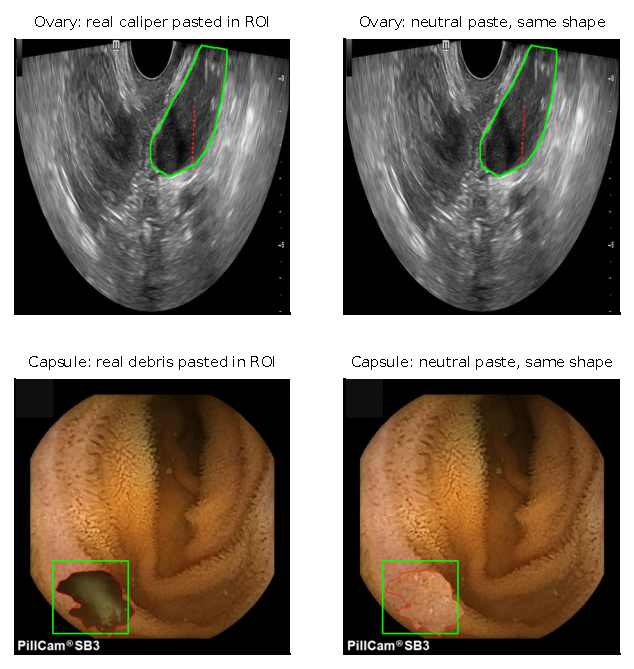
\includegraphics[width=0.60\linewidth]{../stage4_causal_checks/figures/transplant_examples.pdf}
\caption{Transplant and neutral paste on the same recipient images (openly licensed cohorts; MMOTU, SEE-AI CC BY 4.0).
Left: a real artifact instance pasted inside the ROI (\textcolor{roigreen}{green}; the pasted region outlined in
\textcolor{artred}{red}). Right: the neutral paste --- same mask shape and compositing, filled with artifact-free tissue
from the donor.}\label{s4:fig:tx}\end{figure}
Pasting the same real instance outside versus inside the ROI yields a positive location interaction in every cohort
(Table~\ref{s4:tab:tx}; dermoscopy \sFourTIHair, thyroid \sFourTIThy, ovary \sFourTIOv, capsule \sFourTICap; Holm over four).
Table~\ref{s4:tab:txdet} shows the mechanism of Stage~2 on real artifacts: outside the ROI masking removes the pasted
artifact completely --- the masked model's correlated and reversed AUROC coincide (e.g.\ thyroid \sFourMaskCorrOutThy{}
and \sFourMaskRevOutThy) and $|\Delta p|=0$ --- whereas inside it the artifact survives, and for thyroid, ovary and capsule
the masked model reacts to it \emph{more} than ERM (capsule \sFourDpMaskInCap{} versus \sFourDpErmInCap). Group balancing
has a small location interaction of the opposite sign (e.g.\ \sFourTBalHair{} for hair), much smaller than
masking's: it is nearly location-invariant.
\begin{table}[H]\centering\scriptsize
\caption{Real-artifact transplant (T1): the same real artifact instance, cut from a donor image, pasted outside and inside the ROI of the same artifact-free recipient images. These effects combine the artifact with the paste itself (seam, occluded tissue); Table~\ref{s4:tab:neutral} separates them.}\label{s4:tab:tx}
\resizebox{\linewidth}{!}{\begin{tabular}{lcccc}\toprule
Cohort & mask $-$ ERM, pasted outside ROI & pasted inside ROI & Location interaction & Balanced: interaction \\\midrule
ISIC hair & $+0.178$ [$+0.128, +0.227$] & $-0.075$ [$-0.114, -0.036$] & $+0.253$ [$+0.214, +0.293$] & $-0.052$ [$-0.071, -0.033$] \\
Thyroid & $+0.349$ [$+0.321, +0.379$] & $+0.072$ [$+0.043, +0.100$] & $+0.277$ [$+0.256, +0.298$] & $-0.016$ [$-0.025, -0.007$] \\
Ovary & $+0.064$ [$+0.001, +0.126$] & $-0.010$ [$-0.075, +0.056$] & $+0.074$ [$+0.044, +0.104$] & $-0.011$ [$-0.025, +0.002$] \\
Capsule & $+0.322$ [$+0.262, +0.384$] & $-0.175$ [$-0.241, -0.109$] & $+0.497$ [$+0.427, +0.567$] & $-0.032$ [$-0.068, +0.004$] \\
\bottomrule\end{tabular}}
\end{table}

\begin{table}[H]\centering\scriptsize
\caption{Transplant, per location: correlated and reversed AUROC of ERM and of the masked model, and the same-head counterfactual sensitivity to the pasted artifact (T3). Outside the ROI the masked model's correlated and reversed AUROC coincide and $|\Delta p|=0$: the pasted artifact is gone.}\label{s4:tab:txdet}
\resizebox{\linewidth}{!}{\begin{tabular}{lcccccc}\toprule
Cohort & Recipients & ERM in: corr / rev & mask in: corr / rev & mask out: corr / rev & $|\Delta p|$ in: ERM / mask & $|\Delta p|$ out: mask \\\midrule
ISIC hair & 860 & 0.904 / 0.454 & 0.842 / 0.379 & 0.716 / 0.716 & 0.340 / 0.297 & 0.000 \\
Thyroid & 1800 & 0.851 / 0.487 & 0.906 / 0.559 & 0.846 / 0.846 & 0.206 / 0.271 & 0.000 \\
Ovary & 348 & 0.771 / 0.657 & 0.825 / 0.647 & 0.750 / 0.750 & 0.037 / 0.116 & 0.000 \\
Capsule & 340 & 0.906 / 0.508 & 0.956 / 0.333 & 0.914 / 0.914 & 0.238 / 0.551 & 0.000 \\
\bottomrule\end{tabular}}
\end{table}


\paragraph{How much of it is the artifact?} The neutral paste reproduces \sFourShareMin{} to \sFourShareMax{} of the
interaction (Table~\ref{s4:tab:neutral}). Pasting \emph{anything} into the ROI changes what masking does, because the
environments make the pasted region label-correlated whatever it contains: the neutral paste becomes a shortcut
itself (ERM learns it), and masking keeps it only when it lies inside the ROI. Only the difference between the two ---
N3, the interaction with the real artifact minus the interaction with the neutral paste --- is attributable to the
artifact's content: dermoscopy \sFourNThreeHair, thyroid \sFourNThreeThy, ovary \sFourNThreeOv{} and capsule
\sFourNThreeCap{} (\sFourNNThreePos{} of 4 excluding zero). By the registered decision rule (N3 significant \emph{and}
neutral share below one quarter) the transplant signal is not attributable to the artifact alone in any cohort.
\paragraph{What the transplant does and does not show} It shows that on \emph{fixed images}, where a label-correlated
pattern sits decides what masking removes: the image-population explanation of Q4a is excluded. It does \emph{not} give
the harm of a real artifact in its natural context: the effect of masking with pasted hair inside the lesion combines the
hair with the paste and is not attributed to real hair. For hair specifically, the transplant constructs a
pixel-carried shortcut, whereas natural hair is largely correlate-carried (Stage~3).
\begin{table}[H]\centering\scriptsize
\caption{Paste-edge control (R5): the same mask shape and compositing, filled with the donor's own artifact-free tissue. Only the N3 column --- the interaction with the real artifact minus the interaction with the neutral paste --- is attributable to the artifact's content.}\label{s4:tab:neutral}
\resizebox{\linewidth}{!}{\begin{tabular}{lccccc}\toprule
Cohort & mask $-$ ERM, neutral outside & neutral inside & Neutral interaction & Artifact $-$ neutral (N3) & Neutral / artifact interaction \\\midrule
ISIC hair & $+0.129$ [$+0.079, +0.181$] & $-0.075$ [$-0.116, -0.035$] & $+0.204$ [$+0.164, +0.244$] & $+0.049$ [$+0.026, +0.072$] & 81\% \\
Thyroid & $+0.200$ [$+0.175, +0.226$] & $+0.055$ [$+0.028, +0.081$] & $+0.145$ [$+0.130, +0.161$] & $+0.132$ [$+0.116, +0.148$] & 52\% \\
Ovary & $+0.072$ [$+0.009, +0.135$] & $+0.019$ [$-0.041, +0.080$] & $+0.052$ [$+0.021, +0.084$] & $+0.022$ [$-0.002, +0.048$] & 71\% \\
Capsule & $+0.215$ [$+0.154, +0.280$] & $-0.244$ [$-0.314, -0.174$] & $+0.459$ [$+0.383, +0.535$] & $+0.037$ [$-0.017, +0.093$] & 92\% \\
\bottomrule\end{tabular}}
\end{table}


\subsubsection{Robustness of the crossover}
\paragraph{Artifact-label definition} Table~\ref{s4:tab:labsens}. With only large caliper detections, which are almost
certainly real calipers, the crossover is \sFourSensdinoFiveOneEightsenspxFiveZeroThyroid{} (thyroid) and
\sFourSensdinoFiveOneEightsenspxFiveZeroOvary{} (ovary); with strict location thresholds
\sFourSensdinoFiveOneEightsensstrictlocThyroid{} and \sFourSensdinoFiveOneEightsensstrictlocOvary. It keeps its sign and
significance in every variant and grows for the ovary, as expected if detector errors dilute rather than create the
effect. For capsule, a Trap~B that also excludes debris covering part of the lesion box gives
\sFourSensdinoFiveOneEightsensstrictBCapsule{} --- smaller than the main \sFourXCap{} (the strict Trap~B has far fewer
benign images) but clearly positive; the expectation that the main definition was conservative was not confirmed.
\begin{table}[H]\centering\scriptsize
\caption{Sensitivity of the crossover to the definition of the artifact label (registered before running): only large detections, stricter location thresholds, and for capsule a Trap~B that also requires debris to cover less than 5\% of the lesion box.}\label{s4:tab:labsens}
\begin{tabular}{lccc}\toprule
Cohort & Artifact-label definition & Artifact images A / B & Crossover \\\midrule
Thyroid & main & 1150 / 326 & $+0.239$ [$+0.196, +0.280$] \\
Thyroid & large markers ($\ge50$ px) & 1083 / 274 & $+0.244$ [$+0.199, +0.289$] \\
Thyroid & strict location ($r\ge0.7$ / $r<0.05$) & 919 / 298 & $+0.212$ [$+0.164, +0.259$] \\
Ovary & main & 617 / 194 & $+0.170$ [$+0.087, +0.252$] \\
Ovary & large markers ($\ge50$ px) & 609 / 183 & $+0.188$ [$+0.108, +0.266$] \\
Ovary & strict location ($r\ge0.7$ / $r<0.05$) & 571 / 186 & $+0.196$ [$+0.117, +0.277$] \\
Capsule & main & 816 / 1240 & $+0.377$ [$+0.327, +0.426$] \\
Capsule & strict Trap B (lesion coverage $<5\%$) & 816 / 373 & $+0.255$ [$+0.153, +0.349$] \\
\bottomrule\end{tabular}
\end{table}

\paragraph{Leakage without patient identifiers} TN3K, MMOTU and SEE-AI publish no patient or video identifiers, so the
main analysis groups near-duplicates by perceptual hash (and, for capsule, frame blocks). A stricter grouping joins images
whose DINOv2 embeddings are near-identical (Table~\ref{s4:tab:emb}). Raw embedding cosine was dominated by the shared
ultrasound appearance (median nearest-neighbour similarity 0.99 in the ovary), so embeddings were mean-centred per cohort
--- a change recorded before any model was refitted. The crossover is unchanged: thyroid \sFourEmbThyroid, ovary
\sFourEmbOvary, capsule \sFourEmbCapsule. Embedding groups remain a proxy for patient identity: they remove visually
near-identical images, not different-looking images of one patient.
\begin{table}[H]\centering\scriptsize
\caption{Stricter leakage groups for the cohorts without patient identifiers: images joined whenever their (mean-centred) DINOv2 embeddings have cosine $\ge\tau$, united with the existing groups; $\tau$ is the most aggressive grid value that keeps the largest group below 5\% of the cohort (chosen without labels).}\label{s4:tab:emb}
\resizebox{\linewidth}{!}{\begin{tabular}{lccccc}\toprule
Cohort & Leakage groups & cosine $\tau$ & largest group & Crossover, pHash groups & Crossover, embedding groups \\\midrule
Thyroid & 3,455 $\to$ 3,081 & 0.80 & 4.6\% & $+0.239$ [$+0.196, +0.280$] & $+0.235$ [$+0.193, +0.275$] \\
Ovary & 1,059 $\to$ 969 & 0.80 & 2.1\% & $+0.170$ [$+0.087, +0.252$] & $+0.157$ [$+0.053, +0.255$] \\
Capsule & 137 $\to$ 135 & 0.93 & 3.7\% & $+0.377$ [$+0.327, +0.426$] & $+0.353$ [$+0.296, +0.410$] \\
\bottomrule\end{tabular}}
\end{table}

\paragraph{Rebuild on a second machine} Table~\ref{s4:tab:rebuild}. After every dataset was downloaded again and every
derived object rebuilt on different hardware, each crossover reproduces within 0.01 (registered tolerance 0.03). The
re-trained lesion U-Net changed hair-trap membership by about 3\%, and the retrained debris probe moved a handful of
frames across the 3\%/10\% thresholds; neither matters. All intervals in Stages~3--4 come from the rebuilt data.
\begin{table}[H]\centering\small
\caption{Reproduction of the four crossovers after every dataset was re-downloaded and every derived object (lesion U-Net, detectors, probe, groups, caches) rebuilt on a second machine (registered criterion: same sign, CI excluding 0, $|\Delta|\le0.03$).}\label{s4:tab:rebuild}
\begin{tabular}{lccc}\toprule
Cohort & First build (point) & Rebuilt data, second machine & $|\Delta|$ \\\midrule
ISIC hair & $+0.145$ & $+0.147$ [$+0.111, +0.185$] & 0.003 \\
Thyroid & $+0.230$ & $+0.239$ [$+0.196, +0.280$] & 0.009 \\
Ovary & $+0.170$ & $+0.170$ [$+0.087, +0.252$] & 0.001 \\
Capsule & $+0.368$ & $+0.377$ [$+0.327, +0.426$] & 0.008 \\
\bottomrule\end{tabular}
\end{table}


\subsubsection{Sensitivity to the interval estimator}
On the analyses of this stage (Table~\ref{s4:tab:estcheck}, Figure~\ref{s4:fig:width}) the crossed intervals are wider by a
median factor of \sFourEstMed; \sFourEstLost{} of \sFourEstN{} contrasts lose significance (Table~\ref{s4:tab:estchanges}),
none of them a crossover, matched crossover or transplant interaction of masking.
\begin{figure}[H]\centering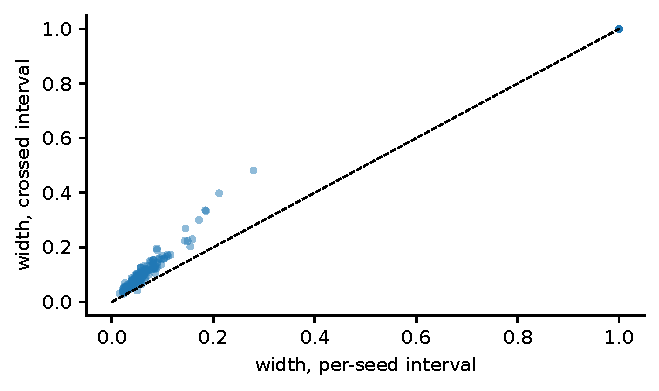
\includegraphics[width=0.52\linewidth]{../stage4_causal_checks/figures/width_scatter.pdf}
\caption{Width of each crossed interval against the per-seed interval of the same contrast (dashed: equal width).}
\label{s4:fig:width}\end{figure}
\begin{table}[H]\centering\scriptsize
\caption{The analyses of this stage under the per-seed and the crossed estimator (same predictions; baseline arms only).}\label{s4:tab:estcheck}
\begin{tabular}{p{5.0cm}p{1.4cm}p{2.6cm}p{2.6cm}p{2.4cm}}\toprule
Result group & Intervals & Excluded 0 only with the per-seed estimator & Excluded 0 only with the crossed estimator & Median width ratio (crossed / per-seed) \\\midrule
capsule/\allowbreak{}dino518\_emb\_groups & 9 & 0 & 0 & 2.02 \\
capsule/\allowbreak{}dino518\_matched & 5 & 0 & 0 & 1.75 \\
capsule/\allowbreak{}dino518\_matched05 & 5 & 0 & 0 & 1.72 \\
capsule/\allowbreak{}dino518\_repro & 5 & 0 & 0 & 1.50 \\
capsule/\allowbreak{}dino518\_sens\_strictB & 9 & 0 & 0 & 1.66 \\
ovary/\allowbreak{}dino518\_emb\_groups & 9 & 0 & 0 & 1.55 \\
ovary/\allowbreak{}dino518\_matched & 5 & 0 & 0 & 1.51 \\
ovary/\allowbreak{}dino518\_matched05 & 5 & 0 & 0 & 1.52 \\
ovary/\allowbreak{}dino518\_repro & 5 & 0 & 0 & 1.55 \\
ovary/\allowbreak{}dino518\_sens\_px50 & 9 & 0 & 0 & 1.62 \\
ovary/\allowbreak{}dino518\_sens\_strictloc & 9 & 0 & 0 & 1.59 \\
review2/\allowbreak{}transplant & 60 & 1 & 0 & 1.63 \\
spec\_e13/\allowbreak{}dino518\_matched & 9 & 0 & 0 & 1.65 \\
spec\_e13/\allowbreak{}dino518\_matched05 & 9 & 1 & 0 & 1.63 \\
spec\_e13/\allowbreak{}dino518\_repro & 9 & 0 & 0 & 1.71 \\
thyroid/\allowbreak{}dino518\_emb\_groups & 9 & 0 & 0 & 1.56 \\
thyroid/\allowbreak{}dino518\_matched & 5 & 0 & 0 & 1.67 \\
thyroid/\allowbreak{}dino518\_matched05 & 5 & 0 & 0 & 1.69 \\
thyroid/\allowbreak{}dino518\_repro & 5 & 0 & 0 & 1.76 \\
thyroid/\allowbreak{}dino518\_sens\_px50 & 9 & 0 & 0 & 1.58 \\
thyroid/\allowbreak{}dino518\_sens\_strictloc & 9 & 1 & 0 & 1.63 \\
\textbf{all} & 204 & 3 & 0 & 1.63 \\
\bottomrule\end{tabular}
\end{table}

\begin{table}[H]\centering\scriptsize
\caption{Contrasts of this stage whose verdict depends on the estimator.}\label{s4:tab:estchanges}
\begin{tabular}{p{4.2cm}p{5.2cm}p{3.3cm}p{2.6cm}}\toprule
Result & Contrast & Crossed estimate [95\% CI] & Verdict vs per-seed estimator \\\midrule
thyroid/\allowbreak{}dino518\_sens\_strictloc & trapB /\allowbreak{} balanced /\allowbreak{} clean /\allowbreak{} balanced /\allowbreak{} erm & $+0.043$ [$-0.008, +0.091$] & no longer excludes 0 \\
spec\_e13/\allowbreak{}dino518\_matched05 & trapA /\allowbreak{} mask /\allowbreak{} clean /\allowbreak{} all /\allowbreak{} mask /\allowbreak{} erm & $-0.026$ [$-0.053, +0.000$] & no longer excludes 0 \\
review2/\allowbreak{}transplant/\allowbreak{}ovary\_dino518 & 0.0 /\allowbreak{} balanced /\allowbreak{} erm /\allowbreak{} test\_rev & $+0.019$ [$-0.006, +0.046$] & no longer excludes 0 \\
\bottomrule\end{tabular}
\end{table}


\subsection{What failed or changed}
\begin{itemize}[leftmargin=*]\itemsep1pt
\item \textbf{The transplant is mostly a paste effect.} The neutral paste reproduces 52--92\% of the interaction; by the
registered rule the transplant is not attributable to the artifact alone in any cohort. No harm figure from the
transplant is attributed to real artifacts.
\item \textbf{Capsule cannot be matched} under the registered rule; its real-trap crossover is descriptive, and its
location evidence rests on the transplant.
\item \textbf{Stricter matching does not improve within-label balance} (up to 0.18--0.19) and shrinks the crossover by
9--16\%.
\item \textbf{The capsule strict-Trap-B variant} gives a smaller crossover, contrary to the expectation registered with it.
\end{itemize}

\subsection{Anticipated questions}
\paragraph{Why not simply adjust for lesion size in the original traps?} Adjustment without matching extrapolates
where the traps do not overlap (hair SMD above 2); matching first restricts the comparison to images that exist in both
traps, and regression then removes what imbalance remains. Doing both is doubly robust: either step alone being correct
is enough.
\paragraph{Why placement values?} AUROC is not a sum over images, so it cannot be regressed directly. Placement values
decompose it exactly into per-image contributions whose class means reproduce the AUROC, so a regression on them adjusts
the crossover itself.
\paragraph{Why is capsule infeasible?} In-ROI debris goes with large lesion boxes (SMD 2.6); among polyp-like lesions
only 19 matched pairs exist, below the registered minimum of 30.
\paragraph{If a neutral paste gives most of the effect, is the transplant useless?} No. It answers the question it was
designed for --- whether the location effect exists on fixed images --- and the neutral paste answers a second question:
the effect is about \emph{any} label-correlated pattern inside the ROI, of which a real artifact is one example. What it
cannot give is an estimate of harm for a particular real artifact.
\paragraph{Why does the neutral paste become a shortcut?} Because the environments make its presence label-correlated,
and a pasted patch leaves a visible seam and occludes the tissue beneath; the encoder can detect both.
\paragraph{Could unmeasured confounding still explain the real-trap crossover?} In principle, yes; matching and
regression only handle measured covariates. The transplant shows that location alone produces the effect on fixed
images, which makes an unmeasured-confounder explanation unnecessary, but it cannot rule one out for the natural traps.
\paragraph{Why group by embeddings rather than ask for patient identifiers?} The data providers do not publish them.
Embedding groups are the strictest available proxy; they reduced thyroid groups from 3,455 to 3,081 without changing the
result.
\paragraph{Why rebuild everything instead of re-running the models?} Re-running on cached objects tests only the last
step. Rebuilding tests the whole chain --- downloads, masks, detectors, groups, features --- and found two gaps in the
reproduction recipe, which were fixed.

\subsection{Conclusion}
\textbf{Supported.} The real-artifact crossover is not explained by measured covariates: it survives matching (3 of 3
feasible cohorts) and doubly robust adjustment (\sFourNATwoOK{} of \sFourNATwo, Holm). Moving the same real artifact inside
the ROI of fixed images reproduces the location effect in all four cohorts, and for hair and thyroid calipers the
artifact's content adds to the effect of the paste. The crossover is robust to the artifact-label definition, to stricter
leakage groups and to a full rebuild. \textbf{Qualified.} Most of the transplant interaction is produced by the paste
itself; unmeasured confounding of the natural location cannot be excluded; capsule is descriptive.
\textbf{Not supported.} A harm figure for real artifacts from the transplant; the capsule matched analysis.

\subsection{Questions for the supervisor}
\begin{enumerate}\itemsep1pt
\item Is matching plus doubly robust adjustment plus the transplant sufficient causal evidence for the thesis, or should a
negative-control analysis be attempted as well?
\item How should the paste effect be presented: as a limitation of the transplant, or as a finding in itself (any
label-correlated pattern inside the ROI defeats masking)?
\item Should capsule endoscopy remain a primary cohort given that its real-trap crossover is descriptive?
\item Is the embedding-group analysis an acceptable answer to the absence of patient identifiers, or must the
limitation be stated more strongly?
\end{enumerate}


\clearpage
% generated by make_combined.py from stage5_practice_theory/stage5.tex; do not edit
\section{Stage 5 --- Practice, breadth and theory}\label{sec:stage5}

\stagebox{\textbf{In one sentence.} On unaltered test sets masking harms exactly the cases the location law says it
should --- shortcut-conflicting images with an in-ROI artifact --- and on the patient-disjoint thyroid split it lowers
sensitivity at every validation-fixed operating point; the crossover replicates in \sFiveNFrozenPos{} of \sFiveNFrozen{}
frozen encoder--cohort pairs, at three model sizes, in \sFiveNFtPos{} of \sFiveNFt{} fine-tuned networks, in the zero-shot
scores of vision--language models, and on new patients (ISIC 2020, \sFiveExtX); a two-parameter linear-Gaussian model
predicts held-out reversed AUROC with mean error \sFiveTMae, less than half the error of the best heuristic, and explains
why the law holds.}
\subsection{Where this stage starts}
Stages~1--4 established the location law in constructed environments --- a strong artifact--label association in
training and its reversal at test --- showed its mechanism (retention with amplified reliance), and showed that it is not
explained by which images carry the artifact. A clinician will ask two questions that this cannot answer: does it
matter on data as collected, without an imposed association, and at the operating point a clinic would use? A
methodologist will ask two more: is the result a property of one encoder and one training regime, and can it be
predicted rather than only observed? This stage answers all four.

\subsection{Questions}
\begin{enumerate}[label=\textbf{Q5\alph*},leftmargin=*]\itemsep1pt
\item On natural test sets, does masking harm the shortcut-conflicting cases, and does that change clinical
sensitivity at fixed operating points?
\item How broadly does the crossover replicate: encoder families and sizes, end-to-end fine-tuning, untrained
(zero-shot) models, new patients?
\item Can a simple model predict a model's reversed-test AUROC from what is observable without the reversed test --- and
so explain when masking helps?
\end{enumerate}
\paragraph{Design decisions} \emph{Hard pairs.} On a natural test set the artifact--label association is weak, so the
overall AUROC barely moves. Positive--negative pairs are therefore split by whether their artifact status conflicts with
the test set's own association (hard) or follows it (easy); the law predicts harm on hard pairs, where the retained
in-ROI artifact points the wrong way. \emph{Operating points fixed on validation data} (never on test) at five clinically
motivated targets, with thresholds re-estimated in every bootstrap replicate. \emph{A theory judged by held-out error,
not by fit}: the model is fitted to each cell's clean and correlated AUROC and must predict the reversed AUROC it never
saw, against two parameter-free heuristics. Rejected: judging the theory by agreement with simulations drawn from its own
assumptions (circular), and by the correlation of predicted and observed crossovers (a heuristic reaches almost the same
correlation).

\subsection{Methods}
\paragraph{Natural test sets} Models are trained on the natural training distribution (no imposed association).
Thyroid: the official patient-disjoint TNCD split \citep{gong2022acl} (614 test images; in-ROI calipers on 37.6\% of benign
and 24.1\% of malignant training images). Dermoscopy: each source (BCN, HAM, MSK) held out in turn (in-lesion hair on 31\%
of melanomas and 20\% of benign lesions). Capsule: held-out frame-block groups. 5 seeds of a group-safe train/validation
split. $A$ = in-ROI artifact. Arms ERM, masking and group balancing.
\paragraph{Clinical metrics and operating points} AUROC, AUPRC, Brier score, expected calibration error; sensitivity and
specificity at OP1--OP5, overall and among shortcut-conflicting positives (for thyroid: malignant nodules with a caliper
on the nodule).
\paragraph{Replication} Frozen DINOv2 ViT-S/B/L (21/86/304\,M parameters), MedSigLIP-448, ConvNeXt-384 and DermLIP with
linear heads; ResNet-50 and ViT-S/16 fine-tuned end to end (ImageNet initialisation, 224\,px, 8 epochs, AdamW, one-cycle
learning rate $10^{-4}$ or $3\cdot10^{-5}$, head $\times10$, thresholds on clean validation; the five folds of seed 42 are
the bootstrap clusters, 15 clusters for the ovary); zero-shot vision--language scores (cosine to a positive minus a
negative class prompt) of MedSigLIP and DermLIP.
\paragraph{External validation} ISIC 2020 \citep{rotemberg2021isic2020} was run only if a gate registered before any
external label was read held: direct download without an agreement, a research licence, patient identifiers, masks
producible by frozen models, and at least 50 images in every cell. Lesion masks: the existing U-Net (ISIC 2018 Task~1
only). Hair masks: a segmenter trained only on the ISIC 2019 hair masks and frozen before any ISIC 2020 image was scored.
Protocol of the ISIC 2019 traps unchanged; groups = patient identifier.
\paragraph{Theory} A frozen encoder maps an image to a disease block with signal-to-noise ratio $S$, an artifact block with
signal-to-noise ratio $A$, and noise. Training uses $P(A{=}1\mid Y{=}1)=p_1=0.9$ and $P(A{=}1\mid Y{=}0)=p_0=0.1$. An
LDA-optimal linear head (which logistic regression approximates) weights each block by its training signal; the
artifact's effective training signal is
\[\tilde A=\frac{(p_1-p_0)^2A}{1+p_1(1-p_1)A},\qquad
\mathrm{AUROC}_{\text{rev}}=\Phi\!\left(\frac{S-\tilde A}{\sqrt{2(S+\tilde A)}}\right),\]
which rises with $S$ and falls with $\tilde A$; for any test composition $q_y=P(A{=}1\mid Y{=}y)$ the same model gives
the AUROC in closed form (\texttt{docs/THEORY.md}). Its consequences: (1) out-of-ROI masking sets $\tilde A\to0$ and helps
unless it destroys most of the disease signal; (2) in-ROI masking keeps $\tilde A$ and changes $S$ to $S_m$, so it
\emph{harms iff it removes disease-informative context} ($S_m<S$); (3) for the same $S_m$ the crossover is positive for
every $\tilde A>0$; (4) group balancing sets the effective association to zero for the artifact and everything
correlated with it, independently of location; (5) a shortcut carried by correlates that the clean and correlated
environments do not reveal is invisible to the model. \emph{Test}: for every cell (result $\times$ trap or overlap
$\times$ arm) $(S,A)$ is fitted to the observed clean and correlated AUROC and the reversed AUROC is predicted; heuristics
``reversed = clean'' and ``symmetric reversal'' (reversed $=$ clean $-$ (correlated $-$ clean)).

\subsection{Experiments}
\begin{table}[H]\centering\scriptsize
\caption{Experiments of this stage and their registration documents (\texttt{docs/PREREGISTRATION\_<name>.md}). Commit times are set by the committing machine and are not independent proof of order.}\label{s5:tab:exp}
\begin{tabular}{p{3.1cm}p{2.1cm}p{2.4cm}p{3.2cm}p{3.3cm}}\toprule
Experiment & Status & Registration & First commit (local time) & Support criterion \\\midrule
Zero-shot vision--language scores, Z1 & \mixed{} registered (descriptive); crossover test post hoc & TEXT\_\allowbreak{}PROMPT & \texttt{7877e8c}, 2026-09-27 12:21 & correlated $-$ reversed gap reported \\
Natural test sets, N3 (hard pairs) & \ok{} registered & NATURAL & \texttt{74bd243}, 2026-09-27 09:39 & mask $-$ ERM $<0$ on hard pairs \\
Operating points S1--S3 & \ok{} registered & REVIEW2 (R3) & \texttt{29cd0da}, 2026-09-27 18:56 & ``masking lowers sensitivity'' only if S1 and $\ge3$ of OP2--OP5 \\
Thyroid subgroup, $n=$\sFiveNConf{} (S3) & \mixed{} registered test in a post hoc subgroup & REVIEW2 (R3) & \texttt{29cd0da}, 2026-09-27 18:56 & sensitivity loss in the subgroup, CI $<0$ \\
Crossed CIs for the subgroup (R6) & \ok{} registered & REVIEW3 (R6) & \texttt{85da735}, 2026-09-27 23:43 & report the crossed CI \\
Fine-tuned hair model and literature comparison (R4) & \ok{} registered & REVIEW2 (R4) & \texttt{29cd0da}, 2026-09-27 18:56 & crossover CI $>0$; comparison descriptive \\
Encoder scale (S/B/L) & \ok{} registered & SCALE & \texttt{13303b0}, 2026-09-27 14:13 & crossover CI $>0$ at every scale \\
Fine-tuned networks & \ok{} registered & FINETUNE & \texttt{7c8b466}, 2026-09-27 07:06 & crossover CI $>0$ (secondary) \\
DermLIP hair traps & \ok{} registered & ISIC2019\_\allowbreak{}TRAPS & \texttt{76e25d4}, 2026-09-26 13:14 & crossover CI $>0$ \\
Theory as held-out predictor, T1--T4 & \ok{} registered & THEORY\_\allowbreak{}PREDICTION & \texttt{4f78653}, 2026-09-27 13:46 & MAE below both heuristics; crossover signs \\
External validation, X1 (ISIC 2020) & \ok{} registered & FINAL (A4) & \texttt{c45d482}, 2026-09-28 00:35 & gate, then crossover CI $>0$ \\
\bottomrule\end{tabular}
\end{table}


\subsection{Results}
\subsubsection{Natural test sets}
Table~\ref{s5:tab:nat}. On all pairs, masking changes little. On shortcut-conflicting pairs it harms in thyroid
(\sFiveNatthyroidhard), BCN (\sFiveNatisicBCNhard) and MSK (\sFiveNatisicMSKhard), and helps in HAM
(\sFiveNatisicHAMhard); in capsule the interval includes zero (\sFiveNatcapsulehard). Where masking harms the hard pairs,
it helps or is neutral on the easy ones (MSK \sFiveNatisicMSKeasy) --- the signature of a model that still uses an in-ROI
artifact after masking: it gets the aligned cases right for the wrong reason and the conflicting cases wrong. The
registered claim N3 is supported in three of five natural test sets. Group balancing improves on masking for the hard
pairs of thyroid (\sFiveNatBalthyroidhard), BCN (\sFiveNatBalisicBCNhard) and MSK (\sFiveNatBalisicMSKhard), but not on
all pairs and not in capsule (\sFiveNatBalcapsuleall{} on all pairs).
\begin{table}[H]\centering\scriptsize
\caption{Natural test sets: AUROC change from masking on all positive--negative pairs and on the pairs whose artifact status conflicts with (``hard'') or follows (``easy'') the test set's own artifact--label association (DINOv2, crossed CIs).}\label{s5:tab:nat}
\resizebox{\linewidth}{!}{\begin{tabular}{lcccc}\toprule
Test set (no imposed correlation) & $P(A{=}1\mid Y{=}1)$ / $P(A{=}1\mid Y{=}0)$ & mask $-$ ERM, all pairs & shortcut-conflicting pairs & shortcut-aligned pairs \\\midrule
Thyroid (official patient-disjoint split) & 0.331 / 0.434 & $-0.004$ [$-0.048, +0.041$] & $-0.095$ [$-0.165, -0.022$] & $+0.042$ [$-0.011, +0.097$] \\
Dermoscopy, BCN held out & 0.356 / 0.239 & $-0.025$ [$-0.035, -0.016$] & $-0.025$ [$-0.043, -0.008$] & $-0.022$ [$-0.035, -0.008$] \\
Dermoscopy, HAM held out & 0.274 / 0.184 & $+0.031$ [$+0.017, +0.045$] & $+0.050$ [$+0.030, +0.070$] & $+0.004$ [$-0.019, +0.027$] \\
Dermoscopy, MSK held out & 0.109 / 0.074 & $+0.016$ [$-0.007, +0.038$] & $-0.065$ [$-0.111, -0.019$] & $+0.100$ [$+0.056, +0.147$] \\
Capsule (held-out frames) & 0.101 / 0.232 & $+0.077$ [$+0.059, +0.097$] & $+0.021$ [$-0.003, +0.048$] & $+0.071$ [$+0.040, +0.108$] \\
\bottomrule\end{tabular}}
\end{table}


\subsubsection{Clinical consequences: thyroid operating points}
On the official, patient-disjoint thyroid test split the AUROC of ERM and of the masked model is almost the same
(\sFiveThyAucerm{} and \sFiveThyAucmask), but masking lowers sensitivity at every operating point (Table~\ref{s5:tab:opthy},
Figure~\ref{s5:fig:op}): at OP1 by \sFiveSensOPOne{} (from \sFiveThySenserm{} to \sFiveThySensmask) and at OP2--OP5 with
intervals below zero in \sFiveNSensLoss{} of 4. By the decision rule registered before the operating points were computed
(S1 and a loss at $\ge3$ of OP2--OP5), the thesis may say that masking lowers sensitivity on this test set. Specificity
rises: masking moves the operating point, and the loss falls on the malignant nodules whose caliper lies on the nodule.
\paragraph{The subgroup of \sFiveNConf{} malignant nodules} \textbf{Registration status: a pre-registered test inside a
post hoc subgroup --- exploratory confirmation.} The subgroup (malignant nodules with an in-ROI caliper) was defined after
the natural-distribution AUROC results were known; the operating-point test in it was registered before the operating
points were computed. The same \sFiveNConf{} nodules enter every seed. At OP2, sensitivity in this subgroup falls from
\sFiveConfErmOPTwo{} to \sFiveConfMaskOPTwo, a change of \sFiveConfOPTwo. The effect is large and consistent across
operating points; its confirmatory weight is limited by the post hoc subgroup definition.
\begin{table}[H]\centering\scriptsize
\caption{Thyroid, official patient-disjoint test split: effect of masking at five validation-fixed operating points (crossed bootstrap with thresholds re-estimated in every replicate). The subgroup is the malignant nodules with an in-ROI caliper (shortcut-conflicting).}\label{s5:tab:opthy}
\resizebox{\linewidth}{!}{\begin{tabular}{lccccc}\toprule
Operating point (fixed on validation) & Sensitivity ERM $\to$ mask & $\Delta$ sensitivity & $\Delta$ specificity & Sensitivity, conflicting malignant (ERM $\to$ mask) & $\Delta$ in that subgroup \\\midrule
OP1 max.\ balanced accuracy & 0.699 $\to$ 0.424 & $-0.275$ [$-0.435, -0.138$] & $+0.202$ [$+0.115, +0.330$] & 0.703 $\to$ 0.223 & $-0.479$ [$-0.640, -0.313$] \\
OP2 specificity $\ge0.80$ & 0.557 $\to$ 0.355 & $-0.202$ [$-0.300, -0.100$] & $+0.117$ [$+0.059, +0.172$] & 0.549 $\to$ 0.177 & $-0.372$ [$-0.499, -0.236$] \\
OP3 specificity $\ge0.90$ & 0.371 $\to$ 0.219 & $-0.152$ [$-0.253, -0.043$] & $+0.075$ [$+0.029, +0.122$] & 0.336 $\to$ 0.100 & $-0.236$ [$-0.383, -0.089$] \\
OP4 sensitivity $\ge0.80$ & 0.753 $\to$ 0.380 & $-0.373$ [$-0.469, -0.270$] & $+0.278$ [$+0.203, +0.359$] & 0.744 $\to$ 0.197 & $-0.546$ [$-0.671, -0.421$] \\
OP5 sensitivity $\ge0.90$ & 0.869 $\to$ 0.588 & $-0.281$ [$-0.391, -0.178$] & $+0.339$ [$+0.236, +0.425$] & 0.862 $\to$ 0.400 & $-0.462$ [$-0.614, -0.310$] \\
\bottomrule\end{tabular}}
\end{table}

\begin{figure}[H]\centering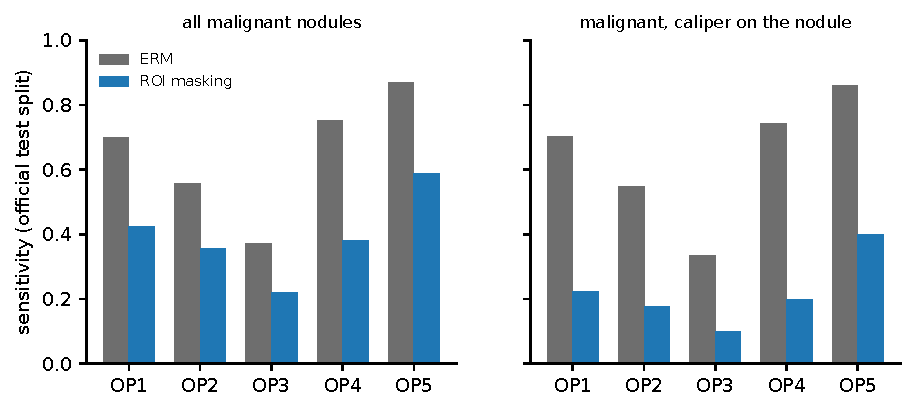
\includegraphics[width=\linewidth]{../stage5_practice_theory/figures/op_thyroid.pdf}
\caption{Thyroid, official patient-disjoint test split: sensitivity of ERM and of the masked model at five
validation-fixed operating points, for all malignant nodules (left) and for the \sFiveNConf{} malignant nodules with a
caliper on the nodule (right; post hoc subgroup, exploratory).}\label{s5:fig:op}\end{figure}
\paragraph{Other test sets} Table~\ref{s5:tab:opother}. At OP2 masking lowers sensitivity, including for the
shortcut-conflicting positives, in the HAM and MSK hold-outs, where it raises specificity; in BCN it lowers specificity; in
capsule it raises sensitivity without a significant change for the conflicting erosions. The thyroid pattern --- a
threshold that no longer catches the positives whose supporting artifact is gone --- recurs in two of the four other
test sets. Table~\ref{s5:tab:clin} gives the threshold-free and
calibration metrics: in thyroid and BCN masking worsens Brier score and calibration; in HAM, MSK and capsule it improves
every metric, matching the AUROC results.
\begin{table}[H]\centering\scriptsize
\caption{Other natural test sets at OP2 (validation specificity $\ge0.80$), mask $-$ ERM, crossed CIs.}\label{s5:tab:opother}
\begin{tabular}{lcccc}\toprule
Test set & Conflicting positives & $\Delta$ sensitivity & $\Delta$ specificity & $\Delta$ sensitivity, conflicting \\\midrule
Dermoscopy BCN & 1832 & $+0.017$ [$-0.003, +0.036$] & $-0.110$ [$-0.135, -0.079$] & $+0.019$ [$-0.004, +0.042$] \\
Dermoscopy HAM & 808 & $-0.062$ [$-0.110, -0.015$] & $+0.092$ [$+0.064, +0.121$] & $-0.055$ [$-0.104, -0.007$] \\
Dermoscopy MSK & 492 & $-0.074$ [$-0.127, -0.026$] & $+0.083$ [$+0.064, +0.110$] & $-0.094$ [$-0.149, -0.044$] \\
Capsule & 38 & $+0.140$ [$+0.082, +0.222$] & $+0.041$ [$-0.029, +0.107$] & $+0.022$ [$-0.041, +0.123$] \\
\bottomrule\end{tabular}
\end{table}

\begin{table}[H]\centering\scriptsize
\caption{Clinical metrics on the natural test sets (seed means; threshold at maximal balanced accuracy on validation data).}\label{s5:tab:clin}
\begin{tabular}{lccccccc}\toprule
Test set & Arm & AUROC & AUPRC & Brier & ECE & Sensitivity & Specificity \\\midrule
Capsule (held-out frames) & ERM & 0.889 & 0.897 & 0.130 & 0.042 & 0.770 & 0.844 \\
 & mask & 0.967 & 0.971 & 0.069 & 0.029 & 0.856 & 0.933 \\
 & balanced & 0.881 & 0.889 & 0.136 & 0.051 & 0.757 & 0.838 \\
ISIC, BCN held out & ERM & 0.786 & 0.587 & 0.238 & 0.279 & 0.842 & 0.521 \\
 & mask & 0.761 & 0.564 & 0.287 & 0.330 & 0.842 & 0.443 \\
 & balanced & 0.782 & 0.587 & 0.229 & 0.260 & 0.835 & 0.509 \\
ISIC, HAM held out & ERM & 0.752 & 0.355 & 0.161 & 0.233 & 0.575 & 0.789 \\
 & mask & 0.782 & 0.396 & 0.138 & 0.199 & 0.569 & 0.831 \\
 & balanced & 0.751 & 0.350 & 0.154 & 0.225 & 0.495 & 0.845 \\
ISIC, MSK held out & ERM & 0.770 & 0.477 & 0.171 & 0.160 & 0.600 & 0.790 \\
 & mask & 0.785 & 0.497 & 0.149 & 0.120 & 0.587 & 0.823 \\
 & balanced & 0.767 & 0.464 & 0.175 & 0.165 & 0.628 & 0.759 \\
Thyroid (official split) & ERM & 0.735 & 0.604 & 0.209 & 0.088 & 0.699 & 0.653 \\
 & mask & 0.731 & 0.629 & 0.215 & 0.119 & 0.424 & 0.856 \\
 & balanced & 0.714 & 0.580 & 0.220 & 0.115 & 0.707 & 0.612 \\
\bottomrule\end{tabular}
\end{table}


\subsubsection{Replication breadth}
Table~\ref{s5:tab:breadth} and Figure~\ref{s5:fig:breadth}. The crossover's interval lies above zero for \sFiveNFrozenPos{} of
\sFiveNFrozen{} frozen encoder--cohort pairs; the exception is DermLIP (Stage~3).
\paragraph{Model scale} Table~\ref{s5:tab:scale}. The law holds at every size in every cohort. Larger models do not escape
the shortcut; they exploit an in-ROI caliper \emph{more}: ERM's correlated$-$reversed gap in the thyroid Trap~A grows
from \sFiveGapthyroidViTS{} (ViT-S) to \sFiveGapthyroidViTB{} (ViT-B) and \sFiveGapthyroidViTL{} (ViT-L), and in the ovary
from \sFiveGapovaryViTS{} to \sFiveGapovaryViTL; capsule is flat.
\begin{table}[H]\centering\scriptsize
\caption{Encoder scale (DINOv2 ViT-S/14 21\,M, ViT-B/14 86\,M, ViT-L/14 304\,M parameters): ERM's shortcut gap in the in-ROI trap and the crossover.}\label{s5:tab:scale}
\begin{tabular}{lcccc}\toprule
Cohort & DINOv2 & ERM clean AUROC (Trap A) & ERM gap corr $-$ rev (Trap A) & Crossover \\\midrule
Thyroid & ViT-S/14 & 0.629 & 0.537 & $+0.247$ [$+0.205, +0.288$] \\
Thyroid & ViT-B/14 & 0.608 & 0.590 & $+0.239$ [$+0.196, +0.280$] \\
Thyroid & ViT-L/14 & 0.601 & 0.622 & $+0.263$ [$+0.218, +0.307$] \\
Ovary & ViT-S/14 & 0.698 & 0.320 & $+0.296$ [$+0.208, +0.384$] \\
Ovary & ViT-B/14 & 0.635 & 0.413 & $+0.170$ [$+0.087, +0.252$] \\
Ovary & ViT-L/14 & 0.608 & 0.564 & $+0.207$ [$+0.127, +0.286$] \\
Capsule & ViT-S/14 & 0.803 & 0.363 & $+0.370$ [$+0.325, +0.415$] \\
Capsule & ViT-B/14 & 0.796 & 0.360 & $+0.377$ [$+0.327, +0.426$] \\
Capsule & ViT-L/14 & 0.820 & 0.347 & $+0.417$ [$+0.369, +0.464$] \\
\bottomrule\end{tabular}
\end{table}

\paragraph{End-to-end fine-tuning} Table~\ref{s5:tab:ftdet}. The crossover replicates in \sFiveNFtPos{} of \sFiveNFt{}
fine-tuned networks: dermoscopy hair with ResNet-50 (\sFiveFtDermoscopyhairResNetFiveZero), thyroid with ViT-S and
capsule with ResNet-50, where masking harms strongly inside the ROI (\sFiveFtACapsuleResNetFiveZero) and helps outside
(\sFiveFtBCapsuleResNetFiveZero). The thyroid ResNet-50 points the same way without significance. The fine-tuned ovary
network is \emph{not evaluable}: with 15 clusters its ERM clean AUROC is \sFiveOvFtCleanA{} (Trap~A) and \sFiveOvFtCleanB{}
(Trap~B) --- it barely learns the task --- so its null says nothing about the law. Fine-tuning does not remove the effect;
it is not an artefact of frozen features.
\begin{table}[H]\centering\scriptsize
\caption{End-to-end fine-tuned networks (ImageNet initialisation, 224\,px, 8 epochs; folds as bootstrap clusters): effect of masking per trap (crossed CIs).}\label{s5:tab:ftdet}
\begin{tabular}{lccc}\toprule
Fine-tuned network & mask $-$ ERM, Trap A & mask $-$ ERM, Trap B & mask+balanced $-$ balanced, Trap A \\\midrule
Dermoscopy hair, ResNet-50 & $-0.002$ [$-0.054, +0.049$] & $+0.141$ [$+0.071, +0.214$] & $-0.008$ [$-0.072, +0.059$] \\
Thyroid, ResNet-50 & $+0.078$ [$+0.032, +0.123$] & $+0.142$ [$+0.073, +0.211$] & $+0.085$ [$+0.035, +0.137$] \\
Thyroid, ViT-S/16 & $+0.122$ [$+0.068, +0.170$] & $+0.244$ [$+0.163, +0.329$] & $+0.059$ [$+0.003, +0.122$] \\
Capsule, ResNet-50 & $-0.279$ [$-0.377, -0.185$] & $+0.327$ [$+0.235, +0.416$] & $-0.020$ [$-0.107, +0.074$] \\
Ovary, ResNet-50 (15 clusters) & $+0.152$ [$+0.070, +0.232$] & $+0.211$ [$+0.090, +0.328$] & \na \\
\bottomrule\end{tabular}
\end{table}

\paragraph{Untrained models} Table~\ref{s5:tab:zs}. Zero-shot scores of vision--language models are already swayed by
artifacts (capsule correlated$-$reversed gap \sFiveZsGapcapsule), and masking changes them according to the law: crossover
thyroid \sFiveZsthyroid, ovary \sFiveZsovary, capsule \sFiveZscapsule{} (borderline), dermoscopy (DermLIP) \sFiveZsisic{}
--- 4 of 4 positive. The effect is therefore a property of the representation, not of the trained head. Caveat:
MedSigLIP's zero-shot thyroid score is at chance (clean AUROC \sFiveZsCleanthyroid), so that row shows artifact effects on
an uninformative score.
\begin{table}[H]\centering\scriptsize
\caption{Zero-shot vision--language scores (no training: cosine to a positive minus a negative class prompt) on the trap test environments, unmasked and masked (crossed CIs). The gap shows the untrained score is already swayed by the artifact; the crossover shows that masking changes it according to the location law.}\label{s5:tab:zs}
\resizebox{\linewidth}{!}{\begin{tabular}{lcccccc}\toprule
Cohort & Model & Zero-shot clean AUROC (Trap A) & Correlated $-$ reversed gap & mask effect, Trap A & mask effect, Trap B & Crossover \\\midrule
Thyroid & MedSigLIP & 0.451 & $+0.072$ & $+0.017$ [$-0.011, +0.045$] & $+0.120$ [$+0.078, +0.162$] & $+0.103$ [$+0.064, +0.143$] \\
Ovary & MedSigLIP & 0.623 & $-0.126$ & $-0.235$ [$-0.289, -0.180$] & $-0.054$ [$-0.135, +0.030$] & $+0.181$ [$+0.103, +0.261$] \\
Capsule & MedSigLIP & 0.631 & $-0.402$ & $+0.004$ [$-0.021, +0.029$] & $+0.049$ [$+0.001, +0.098$] & $+0.045$ [$+0.001, +0.090$] \\
Dermoscopy hair & DermLIP & 0.697 & $+0.082$ & $-0.079$ [$-0.114, -0.044$] & $-0.039$ [$-0.070, -0.008$] & $+0.040$ [$+0.021, +0.058$] \\
\bottomrule\end{tabular}}
\end{table}

\paragraph{New patients} ISIC 2020 met every condition of the registered gate: \sFiveExtImages{} images of
\sFiveExtPatients{} patients, patient-disjoint folds; smallest cell 53 hair-free melanomas (gate 50). The frozen hair
segmenter reaches a hair-free balanced accuracy of 0.93 and pixel IoU 0.60 on held-out ISIC 2019 images. Masking harms with
hair on the lesion (\sFiveExttrapA) and helps with hair beside it (\sFiveExttrapB); the crossover is \sFiveExtX{} (registered
claim X1, supported). Thyroid cohorts with patient identifiers either lack nodule masks (ThyUS2Path
\citep{hou2024thyus2path}, whose scanner interface also triggers the caliper detector) or require a data-use agreement
(TN-SCUI 2020, Stanford AIMI), and were not used; DDTI (134 images) is too small.
\begin{table}[H]\centering\scriptsize
\caption{Replication breadth of the real-artifact crossover (crossed CIs).}\label{s5:tab:breadth}
\begin{tabular}{lccc}\toprule
Cohort & Encoder & Training & Crossover [95\% CI] \\\midrule
Dermoscopy hair & DINOv2 ViT-S/14 & frozen & $+0.163$ [$+0.130, +0.195$] \\
Dermoscopy hair & DINOv2 ViT-B/14 & frozen & $+0.147$ [$+0.111, +0.185$] \\
Dermoscopy hair & DINOv2 ViT-L/14 & frozen & $+0.153$ [$+0.110, +0.195$] \\
Dermoscopy hair & DermLIP & frozen & $+0.014$ [$-0.037, +0.063$] \\
Thyroid & DINOv2 ViT-S/14 & frozen & $+0.247$ [$+0.205, +0.288$] \\
Thyroid & DINOv2 ViT-B/14 & frozen & $+0.239$ [$+0.196, +0.280$] \\
Thyroid & DINOv2 ViT-L/14 & frozen & $+0.263$ [$+0.218, +0.307$] \\
Thyroid & MedSigLIP-448 & frozen & $+0.195$ [$+0.153, +0.238$] \\
Thyroid & ConvNeXt-384 & frozen & $+0.275$ [$+0.231, +0.320$] \\
Ovary & DINOv2 ViT-S/14 & frozen & $+0.296$ [$+0.208, +0.384$] \\
Ovary & DINOv2 ViT-B/14 & frozen & $+0.170$ [$+0.087, +0.252$] \\
Ovary & DINOv2 ViT-L/14 & frozen & $+0.207$ [$+0.127, +0.286$] \\
Ovary & MedSigLIP-448 & frozen & $+0.178$ [$+0.109, +0.248$] \\
Capsule & DINOv2 ViT-S/14 & frozen & $+0.370$ [$+0.325, +0.415$] \\
Capsule & DINOv2 ViT-B/14 & frozen & $+0.377$ [$+0.327, +0.426$] \\
Capsule & DINOv2 ViT-L/14 & frozen & $+0.417$ [$+0.369, +0.464$] \\
Capsule & MedSigLIP-448 & frozen & $+0.335$ [$+0.286, +0.383$] \\
Capsule & ConvNeXt-384 & frozen & $+0.320$ [$+0.268, +0.372$] \\
Dermoscopy hair & ResNet-50 & fine-tuned & $+0.143$ [$+0.054, +0.232$] \\
Thyroid & ResNet-50 & fine-tuned & $+0.063$ [$-0.022, +0.144$] \\
Thyroid & ViT-S & fine-tuned & $+0.122$ [$+0.039, +0.211$] \\
Capsule & ResNet-50 & fine-tuned & $+0.606$ [$+0.495, +0.716$] \\
Ovary & ResNet-50 (15 clusters) & fine-tuned & $+0.058$ [$-0.062, +0.179$] \\
Dermoscopy hair, ISIC 2020 (external) & DINOv2 ViT-B/14 & frozen, new patients & $+0.250$ [$+0.174, +0.327$] \\
\bottomrule\end{tabular}
\end{table}

\begin{figure}[H]\centering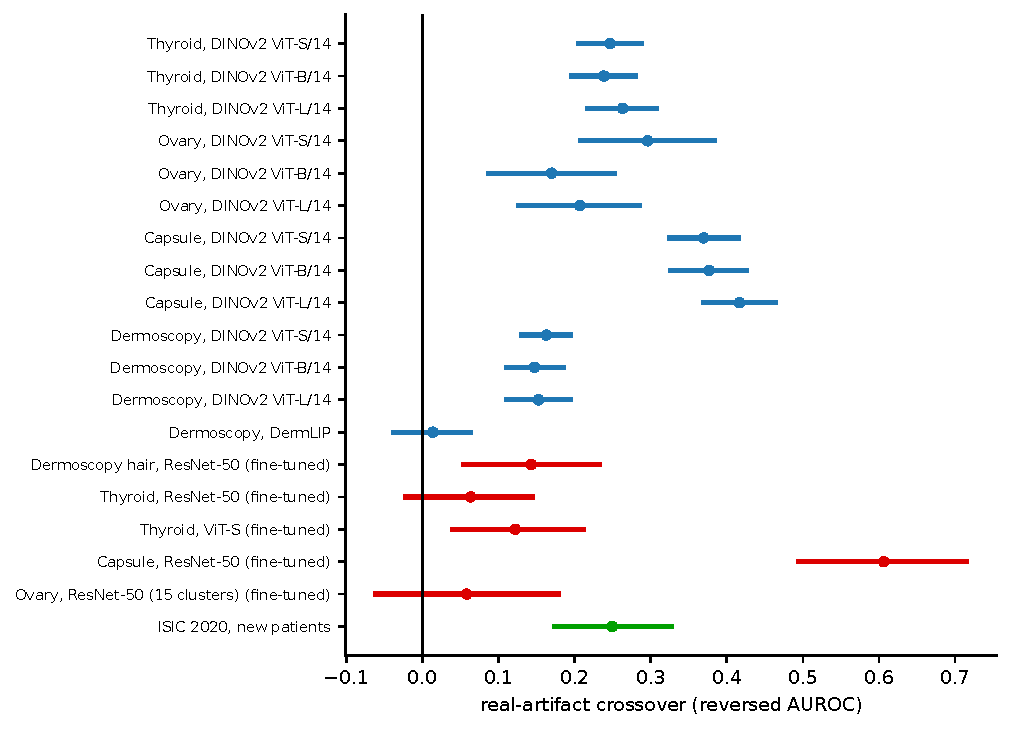
\includegraphics[width=0.8\linewidth]{../stage5_practice_theory/figures/breadth_forest.pdf}
\caption{Crossover across encoders and scales (blue), fine-tuned networks (red) and new patients (green); crossed 95\%
CIs.}\label{s5:fig:breadth}\end{figure}
\paragraph{Absolute performance} Table~\ref{s5:tab:lit}. On the one cohort with a published benchmark on the same
patient-disjoint split, the frozen DINOv2 linear probe reaches an AUROC of \sFiveLitOurs, below published fine-tuned CNNs
(0.77--0.80). The study is about the \emph{relative} effect of masking on a fixed representation, not about
state-of-the-art accuracy, but the gap is a limitation.
\begin{table}[H]\centering\scriptsize
\caption{Absolute performance: the frozen encoder with a linear head against published fine-tuned CNNs on the same patient-disjoint split.}\label{s5:tab:lit}
\begin{tabular}{lcc}\toprule
Model (thyroid, official TNCD test split) & AUROC & Source \\\midrule
ResNet-18, cross-entropy (fine-tuned) & 0.773 & \citet{gong2022acl} \\
DenseNet-121, cross-entropy (fine-tuned) & 0.780 & \citet{gong2022acl} \\
ConvNeXt-T, cross-entropy (fine-tuned) & 0.784 & \citet{gong2022acl} \\
ResNet-18, adaptive curriculum (fine-tuned) & 0.799 & \citet{gong2022acl} \\
DINOv2 ViT-B/14 frozen + linear head, ERM (rebuilt run) & 0.735 & this work \\
\bottomrule\end{tabular}
\end{table}


\subsubsection{The DermLIP exception}
With DermLIP, masking harms at both hair locations (Trap~A \sFiveDermmasktrapAtestrev, Trap~B \sFiveDermmasktrapBtestrev).
Two measurements explain it. First, masking costs DermLIP disease signal wherever the hair lies: clean-test AUROC changes by
\sFiveDermmasktrapAclean{} and \sFiveDermmasktrapBclean. Second, the pixel part of its hair shortcut is small at both
locations (oracle hair inpainting \sFiveDerminpainttrapAtestrev{} and \sFiveDerminpainttrapBtestrev), whereas group
balancing, which also removes correlates of hair, gains \sFiveDermbalancedtrapAtestrev{} and \sFiveDermbalancedtrapBtestrev:
DermLIP carries the hair shortcut mostly through correlates that masking does not remove at either location. In the terms
of the theory, masking lowers $S$ at both locations and removes little of $\tilde A$ at either, so there is no gap to
find. The theory anticipates this from the clean and correlated AUROC alone: predicted crossover \sFiveDermPred, observed
\sFiveDermObs.

\subsubsection{The theory, judged by held-out error}
\begin{figure}[H]\centering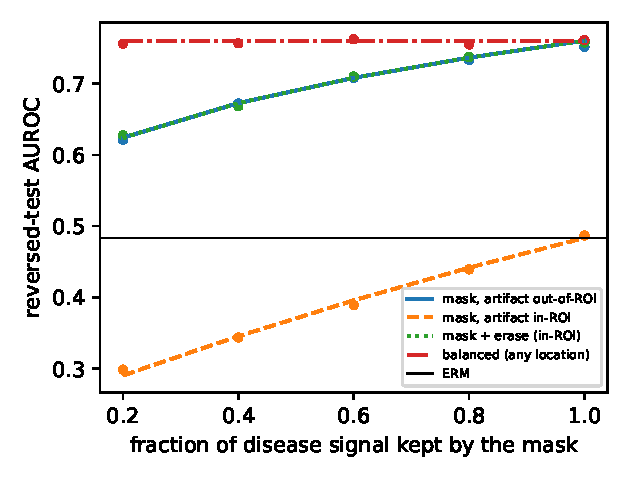
\includegraphics[width=0.55\linewidth]{../../paper/figures/theory.pdf}
\caption{The closed form (lines) against Monte Carlo simulation of its own model (points): the formula is exact up to
simulation noise (at most \sFiveSimMax{} AUROC over \sFiveSimN{} settings). This checks the algebra, not the
theory.}\label{s5:fig:sim}\end{figure}
Table~\ref{s5:tab:theory} and Figure~\ref{s5:fig:theory}. Over \sFiveTN{} primary cells the theory predicts the reversed AUROC
--- never used in fitting --- with mean absolute error \sFiveTMae{} (Pearson $r$ \sFiveTR; \sFiveTWithin{} within 0.05),
against \sFiveTMaeSym{} for the symmetric-reversal heuristic and \sFiveTMaeClean{} for ``reversed = clean''. It gets the
sign of all \sFiveTTwoN{} real-trap crossovers right (MAE \sFiveTTwoMae) and of \sFiveTTwoFt{} fine-tuned crossovers ---
networks that violate its assumptions --- and the sign of \sFiveTThreeSign{} of \sFiveTThreeN{} controlled-sweep gains
(heuristic: \sFiveTThreeSymSign). From the fitted $S$ alone, the sign of the in-ROI masking effect is right in
\sFiveTFourAgree{} of \sFiveTFourN{} cells. Its clear failure is the chest-drain cohort of Stage~3: the clean and
correlated environments do not reveal a shortcut carried by the treated lung, so the model cannot see it --- the boundary
its assumption (5) predicts.

The account is simple: a model's reliance on an artifact is fixed by the ratio of artifact to disease signal it sees;
masking lowers the disease signal (less context) and, when the artifact lies inside the ROI, leaves the artifact's signal
intact, so it raises that ratio exactly when the artifact is inside.
\begin{table}[H]\centering\scriptsize
\caption{Held-out prediction of the reversed-test AUROC (never used in fitting): the two-parameter theory fitted to each cell's clean and correlated AUROC, against two parameter-free heuristics.}\label{s5:tab:theory}
\begin{tabular}{lccccc}\toprule
Cells & Predictor & $n$ & MAE & Pearson $r$ & within 0.05 \\\midrule
Primary cells (ERM, mask) & linear-Gaussian theory & 136 & 0.052 & 0.914 & 66\% \\
 & heuristic: symmetric reversal & 136 & 0.129 & 0.743 & 40\% \\
 & heuristic: reversed = clean & 136 & 0.237 & 0.550 & 18\% \\
All ERM-head arms & linear-Gaussian theory & 598 & 0.036 & 0.933 & 79\% \\
 & heuristic: symmetric reversal & 598 & 0.076 & 0.823 & 65\% \\
 & heuristic: reversed = clean & 598 & 0.151 & 0.584 & 40\% \\
Fine-tuned (outside assumptions) & linear-Gaussian theory & 12 & 0.027 & 0.980 & 92\% \\
\bottomrule\end{tabular}
\end{table}

\begin{figure}[H]\centering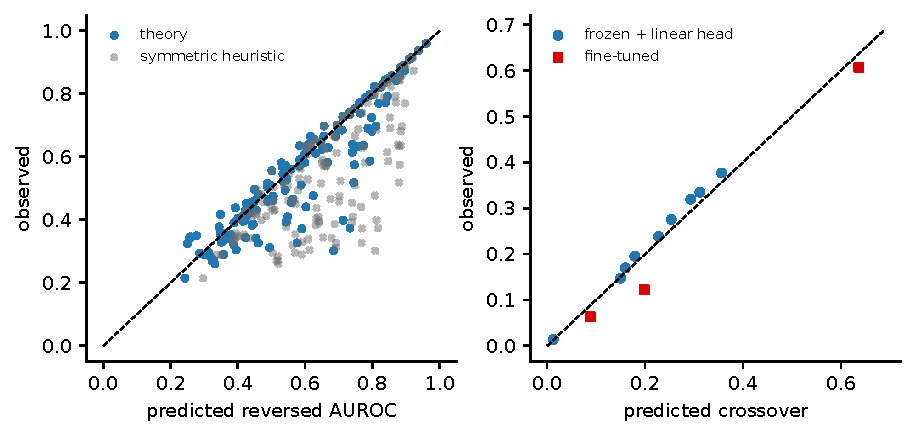
\includegraphics[width=\linewidth]{../stage5_practice_theory/figures/theory_prediction.pdf}
\caption{Left: predicted versus observed reversed AUROC (theory, blue; symmetric heuristic, grey). Right: predicted
versus observed real-trap crossover (frozen encoders, blue; fine-tuned, red).}\label{s5:fig:theory}\end{figure}
\paragraph{Verdict by the registered rule} The rule called the theory \emph{quantitatively predictive} only if every
crossover sign agreed, both correlations were $\ge0.7$, and its error beat ``reversed = clean''. On the full registered
cell set one near-zero chest-radiograph crossover (observed $\approx-0.002$) had the wrong sign; the report therefore calls
it a \emph{qualitative account that closely matches held-out results} and does not say that it ``predicts magnitudes''. The
correlation of predicted and observed crossovers ($r=$ \sFiveTTwoR) is not used as evidence, because the symmetric
heuristic also correlates almost perfectly; the held-out error is the evidence.

\subsubsection{Sensitivity to the interval estimator}
On the analyses of this stage (Table~\ref{s5:tab:estcheck}) the crossed intervals are wider by a median factor of
\sFiveEstMed; \sFiveEstLost{} of \sFiveEstN{} contrasts lose significance and \sFiveEstGained{} gains it
(Table~\ref{s5:tab:estchanges}). The ones that matter for the text --- masking's gain on the easy thyroid pairs and on all MSK
pairs --- are therefore not claimed; natural-set intervals are about twice as wide as the per-seed ones, because every seed
scores the same test images.
\begin{table}[H]\centering\scriptsize
\caption{The analyses of this stage under the per-seed and the crossed estimator (same predictions; baseline arms only).}\label{s5:tab:estcheck}
\begin{tabular}{p{5.0cm}p{1.4cm}p{2.6cm}p{2.6cm}p{2.4cm}}\toprule
Result group & Intervals & Excluded 0 only with the per-seed estimator & Excluded 0 only with the crossed estimator & Median width ratio (crossed / per-seed) \\\midrule
capsule/\allowbreak{}dinol518\_scale & 9 & 1 & 0 & 1.53 \\
capsule/\allowbreak{}dinos518\_scale & 9 & 0 & 0 & 1.38 \\
finetune/\allowbreak{}capsule & 4 & 0 & 0 & 1.10 \\
finetune/\allowbreak{}isic & 4 & 0 & 0 & 1.20 \\
finetune/\allowbreak{}ovary & 2 & 0 & 0 & 1.23 \\
finetune/\allowbreak{}thyroid & 8 & 1 & 1 & 1.17 \\
natural/\allowbreak{}capsule\_dino518\_repro & 6 & 0 & 0 & 1.16 \\
natural/\allowbreak{}isic\_BCN\_dino518\_repro & 6 & 0 & 0 & 1.72 \\
natural/\allowbreak{}isic\_HAM\_dino518\_repro & 6 & 0 & 0 & 1.95 \\
natural/\allowbreak{}isic\_MSK\_dino518\_repro & 6 & 2 & 0 & 2.01 \\
natural/\allowbreak{}thyroid\_dino518\_repro & 6 & 1 & 0 & 2.06 \\
ovary/\allowbreak{}dinol518\_scale & 9 & 1 & 0 & 1.58 \\
ovary/\allowbreak{}dinos518\_scale & 9 & 1 & 0 & 1.56 \\
spec\_e13/\allowbreak{}dinol518\_spec\_scale & 17 & 2 & 0 & 1.44 \\
spec\_e13/\allowbreak{}dinos518\_spec\_scale & 17 & 1 & 0 & 1.61 \\
thyroid/\allowbreak{}dinol518\_scale & 9 & 1 & 0 & 1.59 \\
thyroid/\allowbreak{}dinos518\_scale & 9 & 0 & 0 & 1.37 \\
zero\_shot/\allowbreak{}boot & 12 & 1 & 0 & 2.00 \\
\textbf{all} & 148 & 12 & 1 & 1.53 \\
\bottomrule\end{tabular}
\end{table}

\begin{table}[H]\centering\scriptsize
\caption{Contrasts of this stage whose verdict depends on the estimator.}\label{s5:tab:estchanges}
\begin{tabular}{p{4.2cm}p{5.2cm}p{3.3cm}p{2.6cm}}\toprule
Result & Contrast & Crossed estimate [95\% CI] & Verdict vs per-seed estimator \\\midrule
zero\_shot & medsiglip448 /\allowbreak{} ovary /\allowbreak{} trapB /\allowbreak{} zs\_mask-zs & $-0.054$ [$-0.135, +0.030$] & no longer excludes 0 \\
thyroid/\allowbreak{}dinol518\_scale & trapB /\allowbreak{} balanced /\allowbreak{} clean /\allowbreak{} balanced /\allowbreak{} erm & $+0.036$ [$-0.002, +0.073$] & no longer excludes 0 \\
ovary/\allowbreak{}dinos518\_scale & trapB /\allowbreak{} balanced /\allowbreak{} clean /\allowbreak{} balanced /\allowbreak{} erm & $+0.038$ [$-0.000, +0.077$] & no longer excludes 0 \\
ovary/\allowbreak{}dinol518\_scale & trapB /\allowbreak{} balanced /\allowbreak{} clean /\allowbreak{} balanced /\allowbreak{} erm & $+0.043$ [$-0.002, +0.087$] & no longer excludes 0 \\
capsule/\allowbreak{}dinol518\_scale & trapA /\allowbreak{} mask /\allowbreak{} clean /\allowbreak{} mask /\allowbreak{} erm & $+0.012$ [$-0.006, +0.031$] & no longer excludes 0 \\
spec\_e13/\allowbreak{}dinos518\_spec\_scale & trapB /\allowbreak{} mask /\allowbreak{} clean /\allowbreak{} all /\allowbreak{} mask /\allowbreak{} erm & $+0.028$ [$-0.000, +0.055$] & no longer excludes 0 \\
spec\_e13/\allowbreak{}dinol518\_spec\_scale & trapA /\allowbreak{} mask /\allowbreak{} test\_rev /\allowbreak{} HAM /\allowbreak{} mask /\allowbreak{} erm & $-0.044$ [$-0.090, +0.002$] & no longer excludes 0 \\
spec\_e13/\allowbreak{}dinol518\_spec\_scale & trapB /\allowbreak{} mask /\allowbreak{} clean /\allowbreak{} all /\allowbreak{} mask /\allowbreak{} erm & $-0.025$ [$-0.055, +0.003$] & no longer excludes 0 \\
natural/\allowbreak{}thyroid\_dino518\_repro & easy  /\allowbreak{}  mask-erm & $+0.042$ [$-0.011, +0.097$] & no longer excludes 0 \\
natural/\allowbreak{}isic\_MSK\_dino518\_repro & all  /\allowbreak{}  mask-erm & $+0.016$ [$-0.007, +0.038$] & no longer excludes 0 \\
natural/\allowbreak{}isic\_MSK\_dino518\_repro & all  /\allowbreak{}  balanced-mask & $-0.018$ [$-0.041, +0.005$] & no longer excludes 0 \\
finetune/\allowbreak{}thyroid/\allowbreak{}resnet50 & trapB /\allowbreak{} mask\_balanced /\allowbreak{} balanced & $+0.069$ [$-0.004, +0.143$] & no longer excludes 0 \\
finetune/\allowbreak{}thyroid/\allowbreak{}vit\_small\_patch16\_224.augreg\_in21k\_ft\_in1k & trapA /\allowbreak{} mask\_balanced /\allowbreak{} balanced & $+0.059$ [$+0.003, +0.122$] & now excludes 0 \\
\bottomrule\end{tabular}
\end{table}


\subsection{What failed or changed}
\begin{itemize}[leftmargin=*]\itemsep1pt
\item \textbf{Natural test sets}: N3 holds in three of five; HAM goes the other way and capsule is inconclusive.
\item \textbf{The thyroid subgroup} is a post hoc subgroup; its test was registered only after its AUROC result was known.
\item \textbf{Fine-tuning}: thyroid ResNet-50 is not significant; the ovary network is not evaluable.
\item \textbf{DermLIP}: no crossover; explained, and anticipated by the theory, but still an exception.
\item \textbf{The theory} is a qualitative account by its registered rule and fails for correlate-carried shortcuts (chest
drains); the chest-radiograph cells could not be re-estimated and are excluded from its current error figures.
\item \textbf{Absolute performance} is below task-specific fine-tuned models on thyroid.
\item \textbf{External validation is dermoscopy only}; no ultrasound or capsule cohort passed the gate.
\end{itemize}

\subsection{Anticipated questions}
\paragraph{Why does AUROC barely change on natural data while sensitivity drops by a quarter?} AUROC averages over all
positive--negative pairs, and most pairs do not involve the shortcut. A fixed threshold, however, is set on validation
data where the caliper helps; after masking the model's scores for malignant nodules without a supporting caliper fall
below it. The hard-pair AUROC and the subgroup sensitivity isolate exactly those cases.
\paragraph{Why does masking help on the hard HAM pairs?} This is not explained, and it is reported as a failure of N3
for that test set. A possible reading --- that for HAM-style images the model trained on BCN and MSK relied more on hair
beside the lesion than on hair on it, so that masking removed more shortcut than it kept --- has not been tested.
\paragraph{Why do larger models exploit the caliper more?} A plausible reading, not tested directly, is that they
represent small, high-contrast structures such as caliper crosses more distinctly (a larger $A$ in the theory), so the
linear head finds the shortcut more easily. What is established is only that scale is not a defence.
\paragraph{Why include zero-shot scores whose thyroid AUROC is at chance?} Only to show that the location effect lives in
the representation: even without any head trained on the trap, masking changes the artifact's influence differently
inside and outside the ROI.
\paragraph{Why is ISIC 2020 external if it is also ISIC?} It is a different acquisition campaign with different patients,
patient identifiers and no image overlap; the hair masks and lesion masks were produced by models frozen before any ISIC
2020 image was seen. It is external for patients, not for modality.
\paragraph{Is a two-parameter model with two inputs per cell not trivially accurate?} It has two inputs and predicts a
third quantity it never saw; the heuristics use the same two inputs and are two to four times worse. It also predicts
crossovers, which combine four cells, and signs of in-ROI effects.
\paragraph{Why keep the subgroup result if it is post hoc?} It is the clinically meaningful case --- a malignant nodule the
sonographer measured --- and the test in it was registered before it was computed. It is labelled exploratory everywhere.

\subsection{Conclusion}
\textbf{Supported.} On unaltered data masking harms the shortcut-conflicting cases in three of five test sets and lowers
thyroid sensitivity at every validation-fixed operating point (registered decision rule met). The crossover replicates
across encoder families and sizes, in three of the four evaluable fine-tuned networks, in untrained vision--language
scores and on new patients. A two-parameter theory matches held-out reversed AUROC far better than heuristics, explains
every regime observed so far, and anticipates the DermLIP exception. \textbf{Qualified.} The \sFiveNConf-nodule subgroup
is exploratory confirmation; the theory is a qualitative account by its own rule. \textbf{Not supported.} Harm on natural
HAM and capsule test sets; a crossover for DermLIP and for the thyroid ResNet-50.

\subsection{Questions for the supervisor}
\begin{enumerate}\itemsep1pt
\item Is a sensitivity loss on one patient-disjoint split (thyroid) enough for a clinical claim, or should the thesis
lead with the AUROC on shortcut-conflicting cases?
\item Should the theory be a main contribution (with its held-out error as evidence) or a supporting section?
\item Is ISIC 2020 enough external validation, given that it is the same modality and artifact as the main dermoscopy
analysis?
\item Should the below-benchmark absolute performance of frozen linear probes be addressed with fine-tuned models in the
main text, or is the fine-tuned replication sufficient?
\end{enumerate}


\clearpage
% generated by make_combined.py from stage6_remedies_audit_paper/stage6.tex; do not edit
\section{Stage 6 --- What to do instead of masking, and the state of the thesis}\label{sec:stage6}

\stagebox{\textbf{In one sentence.} What to use instead of masking depends on what carries the shortcut: an
annotation-free mask-then-erase method (U-MtE) repairs artifacts that carry the shortcut in their own pixels (calipers:
thyroid Trap~A \sSixRemThyroidmte{} versus ERM, masking \sSixRemThyroidmask), needs a disease-protection step when the
artifact resembles the pathology (capsule debris), and cannot help when the shortcut is carried by correlates of the
artifact (hair, chest drains), where only label-based reweighting works; with image-level artifact labels, U-MtE with
balancing or masking with DFR is the most robust choice; for fully fine-tuned networks erasure must happen during
training; and no remedy improves on masking uniformly on unaltered data. The thesis manuscript, its number audit, the
CLAIM checklist and a blinded clinician audit package are ready; the audit itself has not been performed.}
\subsection{Where this stage starts}
Stages~1--5 established that ROI masking removes an artifact outside the ROI and concentrates the model on one inside
it; that this is caused by location, not by which images carry the artifact; that it matters on unaltered data and at
clinical operating points; and that a two-parameter model explains it. They also showed three facts that shape any
remedy: label-based methods (balancing, DFR) fix both locations but need image-level artifact labels; removing the
artifact's pixels fails when the artifact resembles the disease (capsule debris); and some shortcuts are carried by
correlates of the artifact rather than its pixels (hair, drains). This stage asks what a practitioner should do instead
of masking, and reports the state of the thesis.

\subsection{Questions}
\begin{enumerate}[label=\textbf{Q6\alph*},leftmargin=*]\itemsep1pt
\item Can an in-ROI shortcut be removed from frozen foundation-model features \emph{without} any artifact annotation ---
no artifact example, mask or label, only the ROI mask that masking already uses?
\item When does such a remedy fail, and which alternative fits which regime?
\item Can the same be done for networks fine-tuned end to end?
\item Does any remedy transfer to unaltered test data?
\item How will the automatic artifact labels be validated by a clinician, and what remains before submission?
\end{enumerate}

\subsection{Method: from insert-then-erase to U-MtE}\label{s6:sec:method}
\paragraph{Idea} Masking leaves exactly one thing to remove: what lies inside the ROI and is not disease. If we knew
the directions in feature space along which an artifact moves an image, we could project them out. The method estimates
those directions by \emph{inserting} artifacts into images and measuring how the features change.
\paragraph{Evolution}
\begin{enumerate}[leftmargin=*]\itemsep1pt
\item \textbf{Insert-then-erase (I2E).} Paste artifact \emph{templates} (e.g.\ real hair strands cut from other images)
into training images, collect the paired feature differences (with minus without), take the subspace $U_k$ holding 90\%
of their held-out energy (cap 64 directions), and erase it: $x\mapsto x-U_kU_k^\top(x-\mu)$; a logistic head is trained on
the erased features. Works, but needs examples of the artifact.
\item \textbf{Mask-then-erase (MtE).} Estimate the subspace on \emph{masked} images (insert, then mask), so that erasure
targets exactly what masking leaves; the head is trained and tested on masked, erased features.
\item \textbf{U-MtE (universal).} Replace the templates by one \emph{generic} procedural overlay library --- thin strokes,
thick bands, solid and translucent patches, blobs, dashed lines, small glyphs; random colour (half grey), opacity,
width and position, half centred in the ROI (Figure~\ref{s6:fig:overlays}) --- used \emph{unchanged} for every artifact,
dataset and modality. It contains no ruler, no caliper and no hair. U-MtE needs no artifact example, mask or label; only
the ROI mask.
\item \textbf{Disease protection.} If the erased subspace overlaps the disease direction, erasure removes disease
evidence. Protection estimates label directions $W$ on the \emph{artifact-free} training images and erases
$\mathrm{orth}\big((I-WW^\top)U_k\big)$, which leaves every protected direction untouched ($w^\top P(x)=w^\top x$). It
needs diagnosis labels of artifact-free images (which any training set has) and no artifact label.
\item \textbf{U-MtE with balancing.} When image-level artifact labels exist, the head is group-balanced.
\end{enumerate}
\paragraph{Why it should work (theory of Stage~5)} Erasure sets the effective artifact signal $\tilde A$ to zero but scales
the disease signal by $1-\rho^2$, where $\rho$ is the overlap between the erased subspace and the disease direction. It
therefore beats in-ROI masking unless $\rho$ is large --- which is the case when the artifact resembles the disease, and
which protection forces to zero along the protected directions. Overlay \emph{augmentation} with the same overlays only
decorrelates the label from the generated overlays, not from the real artifact; erasure removes the whole subspace of
``foreign overlay'' changes, which contains the real artifact's direction when both move the representation in shared
ways. The theory therefore predicts erase $\gg$ augment for overlay-like artifacts.
\begin{figure}[H]\centering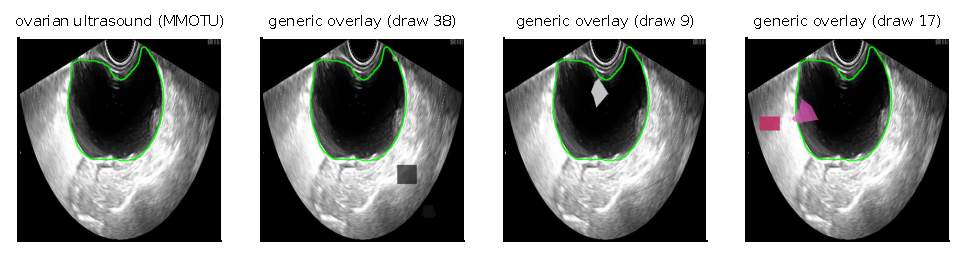
\includegraphics[width=0.9\linewidth]{../stage6_remedies_audit_paper/figures/overlays.pdf}
\caption{The generic overlay library (the same for every modality) drawn on an ovarian ultrasound image (MMOTU, CC BY
4.0; green: ROI). Overlays are inserted, then the image is masked, to estimate the subspace that U-MtE erases.}
\label{s6:fig:overlays}\end{figure}
\paragraph{Baselines} JTT \citep{liu2021jtt} (label-free: up-weight the training errors of an ERM model); SPLINCE
\citep{splice2025} (covariance-preserving linear concept removal with artifact labels; faithful whitened implementation,
verified against the paper's theorem); LEACE (Stages~1 and 3); LaMa inpainting \citep{suvorov2022lama} of the artifact
pixels (needs artifact masks); text-prompted erasure with vision--language models (the artifact direction from a text
description, \citealp{chuang2023debiasing}); SLAS, a few-shot patch-token artifact localiser (5--50 annotated images);
pseudo-group balancing with groups inferred by an overlay detector; erasure followed by DFR; and two validation-driven
selectors that pick, per fold, the candidate with the best worst-group validation score.
\paragraph{Fine-tuned networks} \texttt{mte\_ft}: masked images with and without a generic overlay, plus a penalty on the
distance of their normalised penultimate features; \texttt{umte\_ft} (erase-while-fine-tuning): a running overlay-shift
subspace is estimated on the network's own features and projected out before the head at every step, plus the
invariance penalty; \texttt{cons\_ft}: prediction consistency with and without an overlay; \texttt{umte\_cons\_ft}: all
three; \texttt{mte\_post}: fine-tune like masking, then apply U-MtE to the penultimate features.
\paragraph{Tool} Both methods are packaged for any backbone: \texttt{python -m wtss.umte fit/embed} (images and ROI masks
only) and \texttt{python -m wtss.slas fit/embed} (a few annotated images).

\subsection{Experiments}
\begin{table}[H]\centering\scriptsize
\caption{Experiments of this stage and their registration documents (\texttt{docs/PREREGISTRATION\_<name>.md} or \texttt{docs/<name>.md}). Commit times are set by the committing machine and are not independent proof of order.}\label{s6:tab:exp}
\begin{tabular}{p{3.1cm}p{2.1cm}p{2.4cm}p{3.2cm}p{3.3cm}}\toprule
Experiment & Status & Registration & First commit (local time) & Support criterion \\\midrule
U-I2E / U-MtE, protection, balancing, U7--U14 & \ok{} registered (with amendments before each run) & UNIVERSAL\_\allowbreak{}I2E & \texttt{ee95f10}, 2026-09-26 20:14 & per claim, CI; no gaming (clean loss $\le0.02$, corr $\ge$ rev $-0.02$) \\
Remedy tests P2--P4 in the 16-test family & \mixed{} tests registered; family grouped post hoc & STATISTICAL\_\allowbreak{}PLAN & \texttt{4e9d44c}, 2026-09-27 09:37 & Holm $p<0.05$, estimate $>0$ \\
Erasure-rank ablation & \ok{} registered & UMTE\_\allowbreak{}ABLATION & \texttt{30f19c8}, 2026-09-27 14:15 & descriptive \\
Encoder size (S2) & \ok{} registered & SCALE & \texttt{13303b0}, 2026-09-27 14:13 & protected U-MtE $>$ mask, CI \\
LaMa inpainting & \ok{} registered & INPAINT\_\allowbreak{}LAMA & \texttt{715b790}, 2026-09-27 09:41 & reported with CI, no direction \\
Text-prompted erasure (V1--V3) & \ok{} registered & TEXT\_\allowbreak{}PROMPT & \texttt{7877e8c}, 2026-09-27 12:21 & V1: text erasure $>$ mask \\
SLAS (S0--S6) & \mixed{} registration and localisation result share a commit & SLAS & \texttt{2d1ba20}, 2026-09-26 23:33 & S1: mask-then-suppress $>$ token masking \\
Chest drains (D1--D5) & \ok{} registered & CXR\_\allowbreak{}DRAIN & \texttt{3d0cffc}, 2026-09-27 03:29 & U-MtE $>$ mask, CI \\
Fine-tuning F1--F3 & \ok{} registered & FINETUNE & \texttt{7c8b466}, 2026-09-27 07:06 & mte\_ft $>$ mask, CI \\
Fine-tune, then erase & \ok{} registered & FT\_\allowbreak{}ERASE & \texttt{8ac7a7d}, 2026-09-27 14:20 & mte\_post $>$ mask\_post \\
Erase while fine-tuning (G1--G4) & \ok{} registered (amendments before running) & FT\_\allowbreak{}UMTE & \texttt{b7d7077}, 2026-09-27 14:52 & umte(\_cons)\_ft $>$ mask for both architectures \\
Leakage: embedding groups (P2--P4) & \ok{} registered & EMBEDDING\_\allowbreak{}GROUPS & \texttt{b0eda23}, 2026-09-27 13:55 & same sign and CI verdict \\
Natural data (N1, N2, N4) & \ok{} registered & NATURAL & \texttt{74bd243}, 2026-09-27 09:39 & protected U-MtE $\ge$ mask \\
Clinician image audit (prepared) & \ok{} registered & FINAL (Part B) & \texttt{c45d482}, 2026-09-28 00:35 & precision, recall, location agreement, $\kappa$ \\
\bottomrule\end{tabular}
\end{table}

Every remedy analysis was registered before it was run (\texttt{docs/PREREGISTRATION\_UNIVERSAL\_I2E.md} and its
amendments U7--U14; fine-tuning in \texttt{PREREGISTRATION\_FT\_ERASE.md} and \texttt{PREREGISTRATION\_FT\_UMTE.md}; the
rank ablation, LaMa, text prompts, SLAS and the chest drains in their own documents). Every outcome is reported whichever
way it went.

\subsection{Results}
\subsubsection{Remedies in the real traps}
Figure~\ref{s6:fig:rem} and Table~\ref{s6:tab:rem} (DINOv2, Trap~A); Table~\ref{s6:tab:remall} gives every arm, both traps and
three encoder families.
\begin{itemize}[leftmargin=*]\itemsep1pt
\item \textbf{Calipers (pixel-carried).} Without any annotation, U-MtE repairs most of what masking leaves in thyroid
(\sSixRemThyroidmte{} versus ERM; masking \sSixRemThyroidmask), with MedSigLIP (\sSixRAThyroidMedSigLIPmte) and with ConvNeXt
(\sSixRAThyroidConvNeXtmte), and in the ovary with MedSigLIP (\sSixRAOvarianMedSigLIPmte). With DINOv2 in the ovary its gain
is small (\sSixRemOvarianmte; protected \sSixRemOvarianmteprotect).
\item \textbf{Debris (pathology-like).} Unprotected U-MtE \emph{lowers} capsule performance (\sSixRemCapsulemte; MedSigLIP
\sSixRACapsuleMedSigLIPmte): debris resembles erosion fibrin, so the overlay subspace overlaps the disease. Protection
repairs this (\sSixRemCapsulemteprotect) but does not beat masking; label-based methods are best.
\item \textbf{Hair (correlate-carried).} No pixel-level method helps much (U-MtE \sSixRemDermoscopymte{} versus ERM, i.e.\
\sSixSchairmtemask{} over masking); balancing (\sSixRemDermoscopybalanced) and DFR (\sSixRemDermoscopydfr) are required.
\item \textbf{Outside the ROI} (Trap~B) U-MtE neither helps nor harms relative to masking --- masking has already removed
the artifact.
\end{itemize}
\begin{table}[H]\centering\scriptsize
\caption{Remedies in the in-ROI trap: change in reversed-test AUROC versus ERM (DINOv2, 5 seeds $\times$ 5 folds, crossed CIs). U-MtE needs no artifact annotation; balancing and DFR need image-level artifact labels.}\label{s6:tab:rem}
\resizebox{\linewidth}{!}{\begin{tabular}{lcccccc}\toprule
Cohort (Trap A, in-ROI) & ROI masking & U-MtE & U-MtE protected & group balancing & DFR & U-MtE + balancing \\\midrule
Dermoscopy hair & $-0.049$ [$-0.083, -0.018$] & $-0.009$ [$-0.043, +0.024$] & $-0.008$ [$-0.046, +0.028$] & $+0.213$ [$+0.183, +0.243$] & $+0.196$ [$+0.157, +0.235$] & $+0.185$ [$+0.145, +0.224$] \\
Thyroid calipers & $+0.109$ [$+0.085, +0.133$] & $+0.333$ [$+0.302, +0.364$] & $+0.393$ [$+0.347, +0.434$] & $+0.388$ [$+0.360, +0.418$] & $+0.463$ [$+0.436, +0.492$] & $+0.498$ [$+0.471, +0.524$] \\
Ovarian calipers & $+0.132$ [$+0.072, +0.196$] & $+0.152$ [$+0.098, +0.203$] & $+0.175$ [$+0.116, +0.235$] & $+0.290$ [$+0.248, +0.332$] & $+0.310$ [$+0.263, +0.357$] & $+0.321$ [$+0.271, +0.372$] \\
Capsule debris & $+0.084$ [$+0.055, +0.112$] & $-0.042$ [$-0.076, -0.009$] & $+0.078$ [$+0.047, +0.107$] & $+0.179$ [$+0.150, +0.205$] & $+0.234$ [$+0.199, +0.273$] & $+0.258$ [$+0.221, +0.293$] \\
\bottomrule\end{tabular}}
\end{table}

\begin{figure}[H]\centering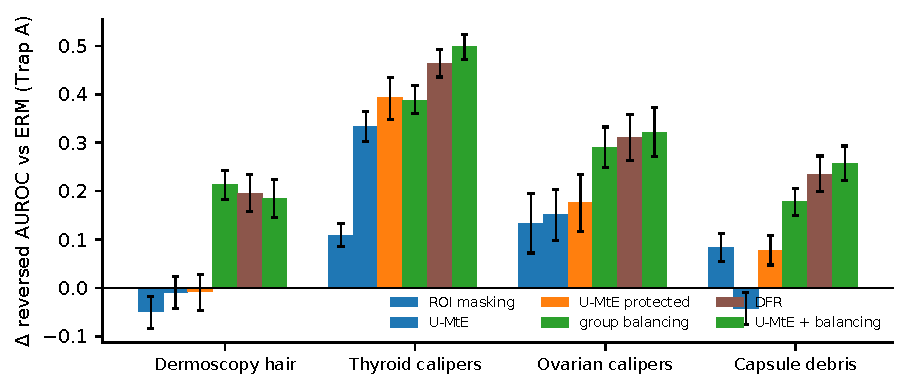
\includegraphics[width=0.9\linewidth]{../stage6_remedies_audit_paper/figures/remedies.pdf}
\caption{Remedies in the in-ROI trap (change in reversed AUROC versus ERM, DINOv2, crossed 95\% CIs).}\label{s6:fig:rem}\end{figure}
{\scriptsize
\begin{longtable}{p{3.4cm}p{4.2cm}p{3.5cm}p{3.5cm}}
\caption{Every remedy in every real-artifact trap and encoder: change in reversed-test AUROC versus ERM (5 seeds $\times$ 5 grouped folds, crossed CIs). U-MtE and the augmentation arm use only the ROI mask; balancing, DFR and their combinations need image-level artifact labels.}\label{s6:tab:remall}\\\toprule
Cohort, encoder & Arm $-$ ERM & Trap A (in ROI) & Trap B (outside) \\\midrule
\endfirsthead
\toprule Cohort, encoder & Arm $-$ ERM & Trap A (in ROI) & Trap B (outside) \\\midrule
\endhead
\bottomrule
\endlastfoot
Dermoscopy hair, DINOv2 & masking & $-0.049$ [$-0.083, -0.018$] & $+0.098$ [$+0.060, +0.136$] \\
 & U-MtE & $-0.009$ [$-0.043, +0.024$] & $+0.121$ [$+0.083, +0.160$] \\
 & U-MtE protected & $-0.008$ [$-0.046, +0.028$] & $+0.124$ [$+0.077, +0.170$] \\
 & same overlays as augmentation & $-0.044$ [$-0.078, -0.012$] & $+0.107$ [$+0.070, +0.145$] \\
 & group balancing & $+0.213$ [$+0.183, +0.243$] & $+0.204$ [$+0.166, +0.245$] \\
 & DFR & $+0.196$ [$+0.157, +0.235$] & $+0.196$ [$+0.147, +0.251$] \\
 & masking + DFR & $+0.152$ [$+0.103, +0.202$] & $+0.206$ [$+0.142, +0.267$] \\
 & U-MtE + balancing & $+0.185$ [$+0.145, +0.224$] & $+0.240$ [$+0.197, +0.283$] \\
Thyroid calipers, DINOv2 & masking & $+0.109$ [$+0.085, +0.133$] & $+0.348$ [$+0.307, +0.388$] \\
 & U-MtE & $+0.333$ [$+0.302, +0.364$] & $+0.347$ [$+0.308, +0.386$] \\
 & U-MtE protected & $+0.393$ [$+0.347, +0.434$] & $+0.349$ [$+0.310, +0.389$] \\
 & same overlays as augmentation & $+0.118$ [$+0.094, +0.143$] & $+0.345$ [$+0.305, +0.385$] \\
 & group balancing & $+0.388$ [$+0.360, +0.418$] & $+0.254$ [$+0.218, +0.292$] \\
 & DFR & $+0.463$ [$+0.436, +0.492$] & $+0.312$ [$+0.262, +0.362$] \\
 & masking + DFR & $+0.537$ [$+0.506, +0.567$] & $+0.357$ [$+0.313, +0.400$] \\
 & U-MtE + balancing & $+0.498$ [$+0.471, +0.524$] & $+0.371$ [$+0.329, +0.412$] \\
Thyroid calipers, MedSigLIP & masking & $+0.053$ [$+0.032, +0.073$] & $+0.248$ [$+0.200, +0.293$] \\
 & U-MtE & $+0.299$ [$+0.270, +0.328$] & $+0.276$ [$+0.232, +0.318$] \\
 & U-MtE protected & $+0.358$ [$+0.330, +0.388$] & $+0.271$ [$+0.224, +0.318$] \\
 & same overlays as augmentation & $+0.074$ [$+0.053, +0.095$] & $+0.248$ [$+0.202, +0.293$] \\
 & group balancing & $+0.409$ [$+0.382, +0.436$] & $+0.201$ [$+0.161, +0.241$] \\
 & DFR & $+0.463$ [$+0.437, +0.489$] & $+0.243$ [$+0.207, +0.282$] \\
 & masking + DFR & $+0.517$ [$+0.490, +0.545$] & $+0.279$ [$+0.234, +0.324$] \\
 & U-MtE + balancing & $+0.505$ [$+0.478, +0.531$] & $+0.313$ [$+0.269, +0.358$] \\
Thyroid calipers, ConvNeXt & masking & $-0.004$ [$-0.029, +0.020$] & $+0.271$ [$+0.228, +0.314$] \\
 & U-MtE & $+0.131$ [$+0.087, +0.171$] & $+0.276$ [$+0.231, +0.320$] \\
 & U-MtE protected & $+0.179$ [$+0.112, +0.236$] & $+0.286$ [$+0.241, +0.332$] \\
 & same overlays as augmentation & $+0.003$ [$-0.021, +0.027$] & $+0.270$ [$+0.227, +0.313$] \\
 & group balancing & $+0.326$ [$+0.305, +0.348$] & $+0.222$ [$+0.186, +0.258$] \\
 & DFR & $+0.369$ [$+0.335, +0.405$] & $+0.260$ [$+0.212, +0.305$] \\
 & masking + DFR & $+0.408$ [$+0.372, +0.442$] & $+0.307$ [$+0.259, +0.354$] \\
 & U-MtE + balancing & $+0.397$ [$+0.362, +0.434$] & $+0.313$ [$+0.266, +0.358$] \\
Ovarian calipers, DINOv2 & masking & $+0.132$ [$+0.072, +0.196$] & $+0.302$ [$+0.225, +0.378$] \\
 & U-MtE & $+0.152$ [$+0.098, +0.203$] & $+0.317$ [$+0.242, +0.388$] \\
 & U-MtE protected & $+0.175$ [$+0.116, +0.235$] & $+0.322$ [$+0.243, +0.398$] \\
 & same overlays as augmentation & $+0.117$ [$+0.054, +0.178$] & $+0.305$ [$+0.224, +0.383$] \\
 & group balancing & $+0.290$ [$+0.248, +0.332$] & $+0.256$ [$+0.190, +0.320$] \\
 & DFR & $+0.310$ [$+0.263, +0.357$] & $+0.278$ [$+0.209, +0.349$] \\
 & masking + DFR & $+0.339$ [$+0.284, +0.393$] & $+0.347$ [$+0.264, +0.428$] \\
 & U-MtE + balancing & $+0.321$ [$+0.271, +0.372$] & $+0.343$ [$+0.265, +0.419$] \\
Ovarian calipers, MedSigLIP & masking & $+0.002$ [$-0.048, +0.051$] & $+0.180$ [$+0.120, +0.238$] \\
 & U-MtE & $+0.212$ [$+0.163, +0.260$] & $+0.191$ [$+0.136, +0.245$] \\
 & U-MtE protected & $+0.155$ [$+0.098, +0.209$] & $+0.166$ [$+0.108, +0.224$] \\
 & same overlays as augmentation & $+0.018$ [$-0.027, +0.062$] & $+0.179$ [$+0.123, +0.235$] \\
 & group balancing & $+0.302$ [$+0.254, +0.351$] & $+0.149$ [$+0.103, +0.197$] \\
 & DFR & $+0.370$ [$+0.320, +0.420$] & $+0.210$ [$+0.154, +0.265$] \\
 & masking + DFR & $+0.356$ [$+0.299, +0.411$] & $+0.229$ [$+0.161, +0.296$] \\
 & U-MtE + balancing & $+0.364$ [$+0.312, +0.416$] & $+0.219$ [$+0.161, +0.277$] \\
Capsule debris, DINOv2 & masking & $+0.084$ [$+0.055, +0.112$] & $+0.461$ [$+0.415, +0.506$] \\
 & U-MtE & $-0.042$ [$-0.076, -0.009$] & $+0.441$ [$+0.396, +0.483$] \\
 & U-MtE protected & $+0.078$ [$+0.047, +0.107$] & $+0.442$ [$+0.397, +0.486$] \\
 & same overlays as augmentation & $+0.096$ [$+0.067, +0.126$] & $+0.462$ [$+0.417, +0.505$] \\
 & group balancing & $+0.179$ [$+0.150, +0.205$] & $+0.244$ [$+0.216, +0.272$] \\
 & DFR & $+0.234$ [$+0.199, +0.273$] & $+0.287$ [$+0.239, +0.335$] \\
 & masking + DFR & $+0.312$ [$+0.275, +0.349$] & $+0.446$ [$+0.393, +0.497$] \\
 & U-MtE + balancing & $+0.258$ [$+0.221, +0.293$] & $+0.471$ [$+0.428, +0.514$] \\
Capsule debris, MedSigLIP & masking & $+0.117$ [$+0.088, +0.147$] & $+0.452$ [$+0.407, +0.495$] \\
 & U-MtE & $-0.113$ [$-0.146, -0.080$] & $+0.406$ [$+0.362, +0.450$] \\
 & U-MtE protected & $+0.088$ [$+0.055, +0.121$] & $+0.448$ [$+0.404, +0.491$] \\
 & same overlays as augmentation & $+0.136$ [$+0.106, +0.166$] & $+0.451$ [$+0.407, +0.495$] \\
 & group balancing & $+0.225$ [$+0.203, +0.248$] & $+0.240$ [$+0.211, +0.269$] \\
 & DFR & $+0.254$ [$+0.222, +0.286$] & $+0.279$ [$+0.242, +0.320$] \\
 & masking + DFR & $+0.345$ [$+0.312, +0.378$] & $+0.438$ [$+0.391, +0.483$] \\
 & U-MtE + balancing & $+0.269$ [$+0.232, +0.308$] & $+0.453$ [$+0.410, +0.496$] \\
Capsule debris, ConvNeXt & masking & $+0.084$ [$+0.049, +0.118$] & $+0.403$ [$+0.358, +0.448$] \\
 & U-MtE & $+0.009$ [$-0.024, +0.040$] & $+0.378$ [$+0.334, +0.422$] \\
 & U-MtE protected & $+0.108$ [$+0.074, +0.142$] & $+0.383$ [$+0.337, +0.429$] \\
 & same overlays as augmentation & $+0.099$ [$+0.066, +0.131$] & $+0.406$ [$+0.361, +0.449$] \\
 & group balancing & $+0.197$ [$+0.172, +0.221$] & $+0.226$ [$+0.198, +0.256$] \\
 & DFR & $+0.255$ [$+0.223, +0.291$] & $+0.293$ [$+0.234, +0.346$] \\
 & masking + DFR & $+0.330$ [$+0.296, +0.364$] & $+0.453$ [$+0.403, +0.502$] \\
 & U-MtE + balancing & $+0.273$ [$+0.231, +0.312$] & $+0.433$ [$+0.384, +0.480$] \\
\end{longtable}}


\subsubsection{Which model is most robust?}
A reversed-test gain can come from inverting the shortcut rather than removing it. Table~\ref{s6:tab:rob} therefore reports
$\min$(reversed, correlated) AUROC. With image-level artifact labels, U-MtE with balancing is the most robust model for
thyroid with all three encoders (e.g.\ \sSixRobThyroidDINOvTwomtebalanced{} with DINOv2) and for the ovary with MedSigLIP
(\sSixRobOvarianMedSigLIPmtebalanced); masking with DFR is best for capsule (\sSixRobCapsuleDINOvTwomaskdfr) and the DINOv2
ovary (\sSixRobOvarianDINOvTwomaskdfr); plain balancing for hair (\sSixRobDermoscopyDINOvTwobalanced) and DFR for chest
drains (\sSixRobChestRADDINOdfr). DFR and masking + DFR over-correct on thyroid: their correlated AUROC falls below the
reversed one (marked $^\dagger$). Without artifact labels, protected U-MtE is the most robust label-free arm for thyroid; for
capsule the best label-free choice is U-MtE combined with JTT (Table~\ref{s6:tab:jtt}).
\begin{table}[H]\centering\scriptsize
\caption{Robustness summary in the in-ROI trap: $\min$(reversed, correlated) AUROC per arm (mean over seeds; best per row in bold; $^\dagger$ = the arm flips the shortcut, correlated $<$ reversed $-0.02$).}\label{s6:tab:rob}
\resizebox{\linewidth}{!}{\begin{tabular}{lcccccccccc}\toprule
Trap A & ERM & mask & U-MtE & U-MtE prot. & overlay aug. & JTT & balanced & DFR & mask+DFR & U-MtE+bal. \\\midrule
Dermoscopy hair, DINOv2 & 0.510 & 0.460 & 0.500 & 0.502 & 0.466 & 0.575 & \textbf{0.722} & 0.705 & 0.662 & 0.695 \\
Thyroid calipers, DINOv2 & 0.289 & 0.398 & 0.622 & 0.682 & 0.407 & 0.417 & 0.677 & 0.669$^\dagger$ & 0.751$^\dagger$ & \textbf{0.787} \\
Thyroid calipers, MedSigLIP & 0.289 & 0.341 & 0.587 & 0.647 & 0.362 & -- & 0.698 & 0.722$^\dagger$ & 0.772$^\dagger$ & \textbf{0.793} \\
Thyroid calipers, ConvNeXt & 0.357 & 0.353 & 0.488 & 0.536 & 0.361 & -- & 0.684 & 0.669$^\dagger$ & 0.713$^\dagger$ & \textbf{0.755} \\
Ovarian calipers, DINOv2 & 0.413 & 0.545 & 0.565 & 0.588 & 0.530 & 0.440 & 0.703 & 0.689$^\dagger$ & \textbf{0.752} & 0.734 \\
Ovarian calipers, MedSigLIP & 0.426 & 0.428 & 0.638 & 0.581 & 0.444 & -- & 0.729 & 0.756$^\dagger$ & 0.782 & \textbf{0.790} \\
Capsule debris, DINOv2 & 0.581 & 0.665 & 0.539 & 0.659 & 0.678 & 0.596 & 0.760 & 0.816 & \textbf{0.892} & 0.839 \\
Capsule debris, MedSigLIP & 0.570 & 0.687 & 0.457 & 0.658 & 0.706 & -- & 0.796 & 0.825 & \textbf{0.915} & 0.839 \\
Capsule debris, ConvNeXt & 0.528 & 0.612 & 0.537 & 0.636 & 0.627 & -- & 0.725 & 0.783 & \textbf{0.858} & 0.801 \\
Chest drains, RAD-DINO & 0.194 & 0.232 & 0.272 & 0.275 & 0.236 & 0.179 & 0.540 & \textbf{0.666} & 0.635 & 0.461 \\
\bottomrule\end{tabular}}
\end{table}


\subsubsection{The 16-test primary family}
Table~\ref{s6:tab:primall}. The four location tests (P1) and twelve remedy tests --- protected U-MtE $>$ mask (P2), erase $>$
augment with the same overlays (P3), U-MtE+balancing $>$ balancing (P4), in each of the four cohorts --- were grouped
into one Holm family after the individual results were known (conservative bookkeeping, not a pre-registered family).
\sSixNPrimOK{} of \sSixNPrim{} are supported: all four P1; P2 in hair, thyroid and ovary (not capsule); P3 in hair and
thyroid (capsule significant in the opposite direction; ovary not after Holm); P4 in thyroid and capsule.
\begin{table}[H]\centering\scriptsize
\caption{The 16-test primary family (DINOv2, Trap~A reversed test unless stated): the four location tests and the twelve remedy tests, Holm-corrected together.}\label{s6:tab:primall}
\resizebox{\linewidth}{!}{\begin{tabular}{lccccc}\toprule
Family & Cohort & Estimate [95\% CI] & $p$ & $p$ (Holm, 16) & Supported \\\midrule
P1 location crossover & ISIC hair (DINOv2) & $+0.147$ [$+0.111, +0.185$] & 0.0001 & 0.0016 & \ok \\
P1 location crossover & Thyroid (DINOv2) & $+0.239$ [$+0.196, +0.280$] & 0.0001 & 0.0016 & \ok \\
P1 location crossover & Capsule (DINOv2) & $+0.377$ [$+0.327, +0.426$] & 0.0001 & 0.0016 & \ok \\
P1 location crossover & Ovary (DINOv2) & $+0.170$ [$+0.087, +0.252$] & 0.0001 & 0.0016 & \ok \\
P2 U-MtE (protected) > mask & ISIC hair & $+0.042$ [$+0.024, +0.058$] & 0.0001 & 0.0016 & \ok \\
P2 U-MtE (protected) > mask & Thyroid & $+0.283$ [$+0.237, +0.329$] & 0.0001 & 0.0016 & \ok \\
P2 U-MtE (protected) > mask & Capsule & $-0.006$ [$-0.018, +0.006$] & 0.2946 & 0.3486 & \no \\
P2 U-MtE (protected) > mask & Ovary & $+0.043$ [$+0.023, +0.065$] & 0.0001 & 0.0016 & \ok \\
P3 erase > augment & ISIC hair & $+0.035$ [$+0.017, +0.055$] & 0.0002 & 0.0016 & \ok \\
P3 erase > augment & Thyroid & $+0.215$ [$+0.189, +0.244$] & 0.0001 & 0.0016 & \ok \\
P3 erase > augment & Capsule & $-0.139$ [$-0.158, -0.120$] & 0.0001 & 0.0016 & \no{} (opposite) \\
P3 erase > augment & Ovary & $+0.035$ [$+0.003, +0.067$] & 0.0326 & 0.1304 & \no \\
P4 U-MtE+balanced > balanced & ISIC hair & $-0.028$ [$-0.064, +0.007$] & 0.1162 & 0.3486 & \no \\
P4 U-MtE+balanced > balanced & Thyroid & $+0.110$ [$+0.079, +0.142$] & 0.0001 & 0.0016 & \ok \\
P4 U-MtE+balanced > balanced & Capsule & $+0.079$ [$+0.042, +0.115$] & 0.0002 & 0.0016 & \ok \\
P4 U-MtE+balanced > balanced & Ovary & $+0.031$ [$-0.014, +0.077$] & 0.1730 & 0.3486 & \no \\
\bottomrule\end{tabular}}
\end{table}


\subsubsection{Remedies in the controlled sweeps}
Tables~\ref{s6:tab:swrem} and~\ref{s6:tab:swisic}. With DINOv2 and RAD-DINO, U-MtE beats masking at full overlap in every modality sweep
(thyroid \sSixSwthyroiddinoFiveOneEightUmte, capsule \sSixSwcapsuledinoFiveOneEightUmte, chest tube
\sSixSwcxrraddinoFiveOneEightUmte).
With MedSigLIP it fails on both the synthetic caliper and the synthetic debris; protection turns the debris failure into
a gain (\sSixSwcapsulemedsiglipProt) but not the caliper failure (\sSixSwthyroidmedsiglipProt). U-MtE with balancing beats
masking in every sweep and has no positive location interaction (dermoscopy: \sSixSwIsicBalInter, against masking's large
positive one). On the dermoscopy ruler, the insert-then-erase precursor on unmasked features helps
(\sSixSwIsicUitwoe) while plain U-MtE does not (\sSixSwIsicUmte): with the
synthetic ruler, the subspace estimated from generic overlays evidently misses the direction of the retained ruler, and
only the balanced variant repairs it.
\begin{table}[H]\centering\scriptsize
\caption{Remedies in the controlled sweeps at full overlap (reversed-test AUROC, crossed CIs).}\label{s6:tab:swrem}
\resizebox{\linewidth}{!}{\begin{tabular}{lcccc}\toprule
Controlled sweep, $r=1$ & U-MtE $-$ mask & U-MtE protected $-$ mask & U-MtE+bal.\ $-$ mask & U-MtE+bal.\ $-$ balanced \\\midrule
Thyroid caliper, DINOv2 & $+0.278$ [$+0.214, +0.344$] & $+0.287$ [$+0.141, +0.464$] & $+0.470$ [$+0.391, +0.550$] & $+0.091$ [$+0.013, +0.172$] \\
Thyroid caliper, MedSigLIP & $-0.076$ [$-0.120, -0.034$] & $-0.041$ [$-0.095, +0.002$] & $+0.458$ [$+0.393, +0.525$] & $+0.069$ [$+0.002, +0.136$] \\
Ovarian caliper, DINOv2 & $+0.140$ [$+0.061, +0.225$] & $+0.114$ [$+0.043, +0.192$] & $+0.251$ [$+0.157, +0.355$] & $-0.032$ [$-0.165, +0.104$] \\
Capsule debris, DINOv2 & $+0.121$ [$+0.078, +0.170$] & $+0.130$ [$+0.083, +0.189$] & $+0.211$ [$+0.134, +0.297$] & $+0.057$ [$-0.008, +0.121$] \\
Capsule debris, MedSigLIP & $-0.190$ [$-0.265, -0.120$] & $+0.114$ [$+0.022, +0.238$] & $+0.299$ [$+0.195, +0.398$] & $-0.018$ [$-0.101, +0.065$] \\
Chest tube, RAD-DINO & $+0.134$ [$+0.113, +0.156$] & $+0.144$ [$+0.125, +0.164$] & $+0.168$ [$+0.145, +0.191$] & $-0.031$ [$-0.042, -0.021$] \\
\bottomrule\end{tabular}}
\end{table}

\begin{table}[H]\centering\scriptsize
\caption{The dermoscopy ruler sweep at full overlap: the insert-then-erase precursor (U-I2E, erasing on unmasked features) and the mask-then-erase variants, versus ERM (crossed CIs).}\label{s6:tab:swisic}
\resizebox{\linewidth}{!}{\begin{tabular}{lcccc}\toprule
Dermoscopy ruler sweep, $r=1$ (DINOv2) & U-I2E $-$ ERM & U-MtE $-$ ERM & U-MtE protected $-$ ERM & U-MtE+bal.\ $-$ ERM \\\midrule
change in reversed AUROC & $+0.197$ [$+0.146, +0.247$] & $-0.007$ [$-0.085, +0.070$] & $+0.091$ [$-0.016, +0.185$] & $+0.243$ [$+0.167, +0.317$] \\
\bottomrule\end{tabular}}
\end{table}


\subsubsection{Erasure versus augmentation, protection, and other contrasts}
Table~\ref{s6:tab:supp}. The \emph{same} overlays used as training augmentation instead of for erasure gain almost nothing
over masking (Table~\ref{s6:tab:remall}, ``same overlays as augmentation''), while erasure gains \sSixScthyroidMedSigLIPmtemteaug{}
over augmentation with MedSigLIP and \sSixScthyroidConvNeXtmtemteaug{} with ConvNeXt on thyroid: it is the subspace
estimation, not exposure to overlays, that helps. Protection is a safety net: it costs nothing on hair
(\sSixSchairmteprotectmte), helps thyroid (\sSixScthyroidmteprotectmte) and removes the capsule failure (protected
$-$ mask \sSixSccapsulemteprotectmask{} versus unprotected \sSixSccapsulemtemask).
\begin{table}[H]\centering\scriptsize
\caption{Secondary remedy contrasts (reversed test, crossed CIs).}\label{s6:tab:supp}
\begin{tabular}{lcc}\toprule
Cohort & Contrast (Trap A) & Estimate [95\% CI] \\\midrule
hair & mte $-$ mask & $+0.040$ [$+0.024, +0.056$] \\
hair & mte\_protect $-$ mte & $+0.001$ [$-0.016, +0.017$] \\
thyroid & mte\_protect $-$ mte & $+0.059$ [$+0.019, +0.096$] \\
thyroid & mte $-$ jtt & $+0.206$ [$+0.171, +0.241$] \\
ovary & mte $-$ jtt & $+0.125$ [$+0.063, +0.189$] \\
thyroid MedSigLIP & mte $-$ mte\_aug & $+0.225$ [$+0.202, +0.247$] \\
thyroid ConvNeXt & mte $-$ mte\_aug & $+0.128$ [$+0.093, +0.161$] \\
thyroid ConvNeXt & mte $-$ mask & $+0.135$ [$+0.102, +0.168$] \\
capsule & mte $-$ mask & $-0.126$ [$-0.146, -0.107$] \\
capsule & mte\_protect $-$ mask & $-0.006$ [$-0.018, +0.006$] \\
\bottomrule\end{tabular}
\end{table}


\subsubsection{How many directions must be erased?}
Table~\ref{s6:tab:rank}. On thyroid the gain is robust for every setting that erases $\ge16$ directions or $\ge50\%$ of the
overlay-shift energy; one to four directions recover only a third of it --- the overlay shift is multi-dimensional. In these
cohorts the 90\% rule reaches the cap of 64 directions. Unprotected erasure harms capsule more the more directions it
removes, as the theory's $\rho$ predicts; the protected variant never harms capsule and helps the ovary at every rank.
\begin{table}[H]\centering\scriptsize
\caption{Erasure-rank ablation (DINOv2, Trap A): reversed-AUROC difference to masking (mean over seeds) for the energy rule (share of held-out overlay-shift energy removed; cap 64) and for fixed ranks $k$.}\label{s6:tab:rank}
\begin{tabular}{lccccc}\toprule
Erased rank & Thyroid U-MtE & Ovary U-MtE & Ovary protected & Capsule U-MtE & Capsule protected \\\midrule
energy 0.50 & $+0.190$ & $-0.003$ & $+0.033$ & $-0.067$ & $-0.006$ \\
energy 0.90 (main) & $+0.224$ & $+0.020$ & $+0.043$ & $-0.126$ & $-0.006$ \\
energy 0.99 & $+0.224$ & $+0.020$ & $+0.043$ & $-0.126$ & $-0.006$ \\
$k=1$ & $+0.068$ & $+0.010$ & $+0.009$ & $+0.001$ & $+0.000$ \\
$k=4$ & $+0.056$ & $-0.038$ & $+0.015$ & $-0.010$ & $-0.003$ \\
$k=16$ & $+0.183$ & $-0.011$ & $+0.020$ & $-0.058$ & $-0.009$ \\
$k=64$ & $+0.224$ & $+0.020$ & $+0.043$ & $-0.126$ & $-0.006$ \\
\bottomrule\end{tabular}
\end{table}


\subsubsection{Encoder size}
Table~\ref{s6:tab:scalerem}. Protected U-MtE beats masking in thyroid and ovary at every DINOv2 size; on capsule protection
is less complete with ViT-L.
\begin{table}[H]\centering\scriptsize
\caption{U-MtE across encoder sizes (crossed CIs).}\label{s6:tab:scalerem}
\begin{tabular}{lccc}\toprule
Cohort & DINOv2 & U-MtE $-$ mask (Trap A) & U-MtE protected $-$ mask \\\midrule
Thyroid & ViT-S/14 & $+0.192$ [$+0.159, +0.227$] & $+0.225$ [$+0.168, +0.276$] \\
Thyroid & ViT-B/14 & $+0.224$ [$+0.195, +0.254$] & $+0.283$ [$+0.237, +0.329$] \\
Thyroid & ViT-L/14 & $+0.246$ [$+0.216, +0.279$] & $+0.274$ [$+0.243, +0.306$] \\
Ovary & ViT-S/14 & $+0.121$ [$+0.084, +0.158$] & $+0.103$ [$+0.074, +0.134$] \\
Ovary & ViT-B/14 & $+0.020$ [$-0.016, +0.054$] & $+0.043$ [$+0.023, +0.065$] \\
Ovary & ViT-L/14 & $+0.094$ [$+0.061, +0.127$] & $+0.060$ [$+0.037, +0.084$] \\
Capsule & ViT-S/14 & $-0.153$ [$-0.172, -0.134$] & $-0.002$ [$-0.018, +0.016$] \\
Capsule & ViT-B/14 & $-0.126$ [$-0.146, -0.107$] & $-0.006$ [$-0.018, +0.006$] \\
Capsule & ViT-L/14 & $-0.097$ [$-0.114, -0.079$] & $-0.044$ [$-0.056, -0.032$] \\
\bottomrule\end{tabular}
\end{table}


\subsubsection{Published baselines and alternatives}
Table~\ref{s6:tab:jtt} (crossed intervals), Table~\ref{s6:tab:regen} (analyses first archived without per-image predictions and
regenerated with them; crossed intervals) and Table~\ref{s6:tab:archived} (point estimates of analyses whose predictions were
not saved).
\begin{itemize}[leftmargin=*]\itemsep1pt
\item \textbf{JTT} (label-free): U-MtE beats it on thyroid (\sSixScthyroidmtejtt) and ovary (\sSixScovarymtejtt); JTT wins
on hair ($\min$(rev, corr) \sSixBlDermoscopyjtt{} versus \sSixBlDermoscopymte); on capsule U-MtE+JTT is the most robust
label-free combination (\sSixBlCapsuleumtejtt).
\item \textbf{SPLINCE} (needs artifact labels): the faithful implementation removes much disease signal (clean AUROC
\sSixBlCleanThyroidsplice{} on thyroid) and still inverts the shortcut on capsule; U-MtE with balancing is more robust
on thyroid, capsule and hair (\sSixBlThyroidmtebalanced{} versus \sSixBlThyroidsplice; \sSixBlCapsulemtebalanced{} versus
\sSixBlCapsulesplice; \sSixBlDermoscopymtebalanced{} versus \sSixBlDermoscopysplice).
\item \textbf{LaMa inpainting} of the detected artifact pixels, followed by masking, is a strong baseline that needs artifact
masks (over masking: thyroid \sSixRgLaMamaskingthyroidmasklamamask, ovary \sSixRgLaMamaskingovarymasklamamask). Protected
U-MtE, which needs no artifact mask, exceeds it on thyroid (\sSixRgLaMamaskingthyroidmteprotectmasklama) and is below it on
ovary (\sSixRgLaMamaskingovarymteprotectmasklama) and hair (\sSixArLaMaisicmteprotectmasklama, archived point estimate);
U-MtE with balancing beats it everywhere. The thyroid comparison changed when the run was regenerated (archived
$-0.009$): the protected arm reproduced about 0.06 higher than in its first run, with unchanged code for that arm, and
now agrees with the protected arm of the main regenerated run (\texttt{results/bootstrap\_correction/archived\_old\_vs\_new.md}).
\item \textbf{Text-prompted erasure} with MedSigLIP and DermLIP is a near no-op ($\le$ \sSixArtextpromptedovarymasktexterasemask{}
over masking): the text-space artifact direction does not coincide with the image-space direction along which the artifact
moves the representation.
\item \textbf{SLAS} localises hair from a few annotated images, but the gain it enables is capped by what hair pixels carry:
removing \emph{every} real hair patch (an oracle) gains only \sSixArSLAShairmtsoracletokmask{} over token-level masking.
\item \textbf{Pseudo-group balancing} from an overlay detector helps on thyroid (reversed \sSixArpseudogroupthyroidumtepbalreversedAUROC{}
versus \sSixArpseudogroupthyroidmtereversedAUROC{} for U-MtE) and not on hair, where the detector cannot see hair.
\item \textbf{Erasure + DFR} adds at most about 0.01 over masking + DFR: once a group-robust head is used, masking does the rest.
\item \textbf{Validation-driven selectors} beat masking in every cohort and are within about 0.02 of the best candidate, but
neither is uniformly best; admitting DFR as a candidate fixes chest drains and makes the choice noisier elsewhere.
\item \textbf{Chest drains}: U-MtE gains \sSixRgchestRADDINOdrainsmtemask{} over masking with RAD-DINO and nothing with
DINOv2 (\sSixRgchestDINOvTwodrainsmtemask); DFR is best.
\item \textbf{Templates instead of generic overlays} on capsule debris make erasure worse
(\sSixRgUMtEtemplatescapsulemtemask{} against masking); disease protection removes that failure
(\sSixRgUMtEtemplatescapsulemteprotectmask).
\end{itemize}
{\scriptsize
\begin{longtable}{lccccc}
\caption{Published baselines: JTT (label-free error upweighting) and SPLINCE (faithful whitened implementation of the covariance-preserving concept projection, needs artifact labels), beside U-MtE (mean over seeds).}\label{s6:tab:jtt}\\\toprule
Cohort (Trap A) & Arm & clean & correlated & reversed & min(rev, corr) \\\midrule
\endfirsthead
\toprule Cohort (Trap A) & Arm & clean & correlated & reversed & min(rev, corr) \\\midrule
\endhead
\bottomrule
\endlastfoot
Thyroid & JTT & 0.629 & 0.829 & 0.417 & 0.417 \\
Thyroid & mask & 0.689 & 0.908 & 0.398 & 0.398 \\
Thyroid & mask+JTT & 0.699 & 0.888 & 0.455 & 0.455 \\
Thyroid & U-MtE & 0.729 & 0.824 & 0.622 & 0.622 \\
Thyroid & U-MtE+JTT & 0.629 & 0.848 & 0.363 & 0.363 \\
Thyroid & balanced & 0.717 & 0.757 & 0.677 & 0.677 \\
Thyroid & mask+SPLINCE & 0.603 & 0.599 & 0.610 & 0.599 \\
Thyroid & U-MtE+bal. & 0.798 & 0.804 & 0.787 & 0.787 \\
Thyroid & U-MtE prot. & 0.728 & 0.769 & 0.682 & 0.682 \\
Thyroid & SPLINCE & 0.577 & 0.565 & 0.587 & 0.565 \\
Capsule & JTT & 0.786 & 0.928 & 0.596 & 0.596 \\
Capsule & mask & 0.860 & 0.972 & 0.665 & 0.665 \\
Capsule & mask+JTT & 0.878 & 0.956 & 0.760 & 0.760 \\
Capsule & U-MtE & 0.815 & 0.972 & 0.539 & 0.539 \\
Capsule & U-MtE+JTT & 0.881 & 0.945 & 0.787 & 0.787 \\
Capsule & balanced & 0.847 & 0.916 & 0.760 & 0.760 \\
Capsule & mask+SPLINCE & 0.786 & 0.715 & 0.852 & 0.715 \\
Capsule & U-MtE+bal. & 0.899 & 0.939 & 0.839 & 0.839 \\
Capsule & U-MtE prot. & 0.855 & 0.970 & 0.659 & 0.659 \\
Capsule & SPLINCE & 0.741 & 0.668 & 0.788 & 0.668 \\
Dermoscopy hair & JTT & 0.745 & 0.898 & 0.564 & 0.564 \\
Dermoscopy hair & mask & 0.712 & 0.916 & 0.454 & 0.454 \\
Dermoscopy hair & mask+JTT & 0.711 & 0.880 & 0.509 & 0.509 \\
Dermoscopy hair & U-MtE & 0.735 & 0.913 & 0.506 & 0.506 \\
Dermoscopy hair & U-MtE+JTT & 0.729 & 0.885 & 0.541 & 0.541 \\
Dermoscopy hair & balanced & 0.785 & 0.850 & 0.722 & 0.722 \\
Dermoscopy hair & mask+SPLINCE & 0.598 & 0.572 & 0.621 & 0.572 \\
Dermoscopy hair & U-MtE+bal. & 0.778 & 0.860 & 0.695 & 0.695 \\
Dermoscopy hair & U-MtE prot. & 0.718 & 0.904 & 0.502 & 0.502 \\
Dermoscopy hair & SPLINCE & 0.600 & 0.575 & 0.637 & 0.575 \\
\end{longtable}}

\begin{table}[H]\centering\scriptsize
\caption{Remedy analyses regenerated with per-image predictions after the other runs (same commands and seeds; crossed bootstrap).}\label{s6:tab:regen}
\begin{tabular}{p{4.0cm}p{2.0cm}p{4.4cm}c}\toprule
Analysis & Cohort & Contrast (Trap A, reversed) & Estimate [95\% CI] \\\midrule
LaMa inpainting then masking & thyroid & mask\_lama $-$ mask & $+0.224$ [$+0.206, +0.242$] \\
 & thyroid & mte\_protect $-$ mask\_lama & $+0.060$ [$+0.013, +0.105$] \\
 & thyroid & mte\_balanced $-$ mask\_lama & $+0.165$ [$+0.146, +0.185$] \\
 & ovary & mask\_lama $-$ mask & $+0.128$ [$+0.084, +0.169$] \\
 & ovary & mte\_protect $-$ mask\_lama & $-0.085$ [$-0.120, -0.050$] \\
 & ovary & mte\_balanced $-$ mask\_lama & $+0.061$ [$+0.026, +0.095$] \\
U-MtE from real-debris templates & capsule & mte $-$ mask & $-0.392$ [$-0.425, -0.360$] \\
 & capsule & mte\_protect $-$ mask & $+0.003$ [$-0.014, +0.021$] \\
chest drains, RAD-DINO & drains & mte $-$ mask & $+0.040$ [$+0.023, +0.057$] \\
 & drains & mte\_protect $-$ mask & $+0.042$ [$+0.028, +0.058$] \\
 & drains & mte $-$ jtt & $+0.094$ [$+0.077, +0.111$] \\
 & drains & mte\_balanced $-$ balanced & $-0.079$ [$-0.106, -0.044$] \\
chest drains, DINOv2 & drains & mte $-$ mask & $-0.001$ [$-0.009, +0.008$] \\
 & drains & mte\_protect $-$ mask & $-0.003$ [$-0.013, +0.006$] \\
 & drains & mte $-$ jtt & $-0.005$ [$-0.021, +0.011$] \\
 & drains & mte\_balanced $-$ balanced & $+0.031$ [$-0.023, +0.079$] \\
\bottomrule\end{tabular}
\end{table}

{\scriptsize
\begin{longtable}{p{4.0cm}p{3.6cm}p{5.2cm}c}
\caption{Remedy analyses whose per-image predictions were not saved, so their intervals could not be re-estimated with the crossed bootstrap: \textbf{point estimates only}.}\label{s6:tab:archived}\\\toprule
Analysis & Cohort / run & Contrast (Trap A, reversed) & Point estimate \\\midrule
\endfirsthead
\toprule Analysis & Cohort / run & Contrast (Trap A, reversed) & Point estimate \\\midrule
\endhead
\bottomrule
\endlastfoot
LaMa inpainting (oracle masks) & isic & lama $-$ mask & $+0.145$ \\
 & isic & mask\_lama $-$ mask & $+0.127$ \\
 & isic & mte\_protect $-$ mask\_lama & $-0.086$ \\
 & isic & mte\_balanced $-$ mask\_lama & $+0.123$ \\
 & isic & lama $-$ erm & $+0.107$ \\
text-prompted erasure & thyroid & mask\_text\_erase $-$ mask & $+0.005$ \\
 & thyroid & mte $-$ mask & $+0.204$ \\
 & thyroid & mask\_text\_erase\_balanced $-$ balanced & $+0.056$ \\
 & ovary & mask\_text\_erase $-$ mask & $+0.008$ \\
 & ovary & mte $-$ mask & $+0.215$ \\
 & ovary & mask\_text\_erase\_balanced $-$ balanced & $-0.010$ \\
 & capsule & mask\_text\_erase $-$ mask & $+0.001$ \\
 & capsule & mte $-$ mask & $-0.236$ \\
 & capsule & mask\_text\_erase\_balanced $-$ balanced & $+0.066$ \\
 & hair (DermLIP) & mask\_text\_erase $-$ mask & $+0.004$ \\
 & hair (DermLIP) & mte $-$ mask & $-0.076$ \\
 & hair (DermLIP) & mask\_text\_erase\_balanced $-$ balanced & $-0.112$ \\
SLAS & hair & tok\_mask $-$ tok\_erm & $+0.030$ \\
 & hair & mts $-$ tok\_mask & $+0.022$ \\
 & hair & slas $-$ tok\_erm & $+0.008$ \\
 & hair & mts\_oracle $-$ tok\_mask & $+0.015$ \\
 & hair & mts\_balanced $-$ tok\_balanced & $+0.051$ \\
 & thyroid & tok\_mask $-$ tok\_erm & $+0.059$ \\
 & thyroid & mts $-$ tok\_mask & $+0.081$ \\
 & thyroid & slas $-$ tok\_erm & $+0.007$ \\
 & thyroid & mts\_oracle $-$ tok\_mask & $+0.047$ \\
 & thyroid & mts\_balanced $-$ tok\_balanced & $+0.070$ \\
erasure + DFR (U10) & thyroid & mte\_dfr $-$ dfr & $+0.101$ \\
 & thyroid & mte\_dfr $-$ mask\_dfr & $+0.007$ \\
 & thyroid & mask\_dfr $-$ dfr & $+0.095$ \\
 & capsule & mte\_dfr $-$ dfr & $+0.080$ \\
 & capsule & mte\_dfr $-$ mask\_dfr & $+0.000$ \\
 & capsule & mask\_dfr $-$ dfr & $+0.080$ \\
 & hair & mte\_dfr $-$ dfr & $-0.039$ \\
 & hair & mte\_dfr $-$ mask\_dfr & $+0.014$ \\
 & hair & mask\_dfr $-$ dfr & $-0.053$ \\
pseudo-group balancing (U8) & thyroid & umte\_pbal reversed AUROC & 0.663 \\
 & thyroid & mte reversed AUROC & 0.622 \\
 & thyroid & pbal reversed AUROC & 0.409 \\
 & thyroid & erm reversed AUROC & 0.289 \\
 & hair & umte\_pbal reversed AUROC & 0.510 \\
 & hair & mte reversed AUROC & 0.506 \\
 & hair & pbal reversed AUROC & 0.498 \\
 & hair & erm reversed AUROC & 0.491 \\
location-adaptive selection (U13) & thyroid & auto $-$ mask & $+0.395$ \\
 & thyroid & auto $-$ dfr & $+0.057$ \\
 & capsule & auto $-$ mask & $+0.168$ \\
 & capsule & auto $-$ dfr & $+0.047$ \\
 & hair & auto $-$ mask & $+0.251$ \\
 & hair & auto $-$ dfr & $-0.038$ \\
 & chest drains & auto $-$ mask & $+0.299$ \\
 & chest drains & auto $-$ dfr & $-0.144$ \\
split-validation selection (U14) & thyroid & auto $-$ mask & $+0.398$ \\
 & thyroid & auto $-$ dfr & $+0.060$ \\
 & capsule & auto $-$ mask & $+0.187$ \\
 & capsule & auto $-$ dfr & $+0.066$ \\
 & ovary & auto $-$ mask & $+0.170$ \\
 & ovary & auto $-$ dfr & $-0.007$ \\
 & hair & auto $-$ mask & $+0.234$ \\
 & hair & auto $-$ dfr & $-0.055$ \\
 & chest drains & auto $-$ mask & $+0.417$ \\
 & chest drains & auto $-$ dfr & $-0.026$ \\
\end{longtable}}


\subsubsection{Robustness of the remedy tests to leakage groups}
Table~\ref{s6:tab:embrem}. With the stricter embedding-based groups of Stage~4, the thyroid remedy tests are unchanged; in the
ovary, erase $>$ augment (P3) and U-MtE+balancing $>$ balancing (P4) lose significance: ``erase beats augment'' is robust in
thyroid and hair but fragile in the ovary.
\begin{table}[H]\centering\scriptsize
\caption{The remedy tests re-run with the stricter embedding-based leakage groups (cohorts without patient identifiers).}\label{s6:tab:embrem}
\begin{tabular}{lccc}\toprule
Cohort & Test & With embedding-based leakage groups & CI $>0$ \\\midrule
Thyroid & P2 U-MtE (protected) > mask & $+0.251$ [$+0.215, +0.284$] & yes \\
Thyroid & P3 erase > augment & $+0.192$ [$+0.160, +0.223$] & yes \\
Thyroid & P4 U-MtE+balanced > balanced & $+0.152$ [$+0.127, +0.177$] & yes \\
Ovary & P2 U-MtE (protected) > mask & $+0.051$ [$+0.020, +0.079$] & yes \\
Ovary & P3 erase > augment & $+0.024$ [$-0.014, +0.062$] & \textbf{no} \\
Ovary & P4 U-MtE+balanced > balanced & $+0.038$ [$-0.005, +0.081$] & \textbf{no} \\
Capsule & P2 U-MtE (protected) > mask & $-0.006$ [$-0.022, +0.014$] & \textbf{no} \\
Capsule & P3 erase > augment & $-0.128$ [$-0.158, -0.098$] & \textbf{no} \\
Capsule & P4 U-MtE+balanced > balanced & $+0.101$ [$+0.071, +0.132$] & yes \\
\bottomrule\end{tabular}
\end{table}


\subsubsection{Fully fine-tuned networks}
Table~\ref{s6:tab:ftrem}. Applying U-MtE \emph{after} fine-tuning does nothing (\sSixFtThyroidResNetFiveZeroMtePost): unconstrained
fine-tuning builds a task-specific caliper feature that generic overlays do not move. Remedies must act \emph{during} training.
Each component alone works for only one architecture on thyroid (invariance for ResNet-50, \sSixFtThyroidResNetFiveZeroMteFt;
prediction consistency for ViT-S, \sSixFtThyroidViTSOneSixConsFt). Combining projection, invariance and consistency
(\texttt{umte\_cons\_ft}, registered before it was run) improves on fine-tuned masking for both: ResNet-50
\sSixFtThyroidResNetFiveZeroUmteConsFt, ViT-S \sSixFtThyroidViTSOneSixUmteConsFt{} --- without any artifact annotation. It fails
on capsule (\sSixFtCapsuleResNetFiveZeroUmteConsFt), the pathology-like regime, and is not significant on the ovary
(\sSixFtOvaryResNetFiveZeroUmteConsFt{} with 15 clusters), where the fine-tuned network barely learns the task.
\begin{table}[H]\centering\scriptsize
\caption{Remedies for end-to-end fine-tuned networks: change in reversed-test AUROC versus fine-tuned masking (last column: versus the same fine-tuned body without erasure). Folds as bootstrap clusters; crossed CIs.}\label{s6:tab:ftrem}
\resizebox{\linewidth}{!}{\begin{tabular}{lccccc}\toprule
Fine-tuned network (Trap A) & invariance (mte\_ft) & erase-while-fine-tuning (umte\_ft) & prediction consistency (cons\_ft) & all three (umte\_cons\_ft) & fine-tune, then erase \\\midrule
Thyroid, ResNet-50 & $+0.139$ [$+0.096, +0.184$] & $+0.186$ [$+0.144, +0.230$] & $+0.042$ [$+0.011, +0.074$] & $+0.195$ [$+0.153, +0.237$] & $-0.000$ [$-0.001, +0.001$] \\
Thyroid, ViT-S/16 & $-0.000$ [$-0.026, +0.026$] & $+0.032$ [$-0.093, +0.144$] & $+0.061$ [$+0.036, +0.084$] & $+0.119$ [$+0.036, +0.198$] & -- \\
Capsule, ResNet-50 & $-0.027$ [$-0.051, -0.006$] & -- & -- & $-0.026$ [$-0.056, +0.006$] & -- \\
Ovary, ResNet-50 (15 clusters) & -- & -- & -- & $+0.045$ [$-0.036, +0.130$] & -- \\
\bottomrule\end{tabular}}
\end{table}


\subsubsection{Unaltered data}
Table~\ref{s6:tab:natrem}. On the natural test sets, of \sSixNatRemN{} remedy--test-set comparisons with masking (all pairs),
\sSixNatRemPos{} favour the remedy and \sSixNatRemNeg{} favour masking; the rest are not significant. Protected U-MtE is
slightly \emph{worse} than masking on the natural thyroid split (the registered claims N1 and N2 were not supported). The
remedies repair the constructed shortcut of the traps; on data where the shortcut is weak, they mostly cost a little.
\begin{table}[H]\centering\scriptsize
\caption{Remedies on the natural test sets (AUROC, all pairs, crossed CIs): no remedy improves on masking uniformly.}\label{s6:tab:natrem}
\resizebox{\linewidth}{!}{\begin{tabular}{lcccc}\toprule
Natural test set & U-MtE $-$ mask & U-MtE protected $-$ mask & balancing $-$ mask & U-MtE + balancing $-$ mask \\\midrule
Thyroid (official split) & $+0.004$ [$-0.012, +0.020$] & $-0.021$ [$-0.034, -0.008$] & $-0.017$ [$-0.064, +0.030$] & $-0.005$ [$-0.023, +0.013$] \\
ISIC, BCN held out & $+0.007$ [$+0.004, +0.010$] & $-0.019$ [$-0.024, -0.014$] & $+0.022$ [$+0.012, +0.031$] & $+0.010$ [$+0.006, +0.015$] \\
ISIC, HAM held out & $+0.013$ [$+0.009, +0.017$] & $-0.006$ [$-0.016, +0.004$] & $-0.032$ [$-0.049, -0.013$] & $+0.018$ [$+0.009, +0.028$] \\
ISIC, MSK held out & $-0.008$ [$-0.014, -0.002$] & $-0.003$ [$-0.012, +0.006$] & $-0.018$ [$-0.041, +0.004$] & $-0.016$ [$-0.024, -0.008$] \\
Capsule (held-out frames) & $-0.005$ [$-0.011, +0.001$] & $-0.023$ [$-0.029, -0.017$] & $-0.086$ [$-0.109, -0.065$] & $-0.008$ [$-0.013, -0.001$] \\
\bottomrule\end{tabular}}
\end{table}


\subsubsection{The decision guide}
\begin{table}[H]\centering\scriptsize
\caption{What carries the shortcut decides the fix.}\label{s6:tab:guide}
\begin{tabular}{p{3.4cm}p{3.4cm}p{4.4cm}p{3.8cm}}\toprule
Regime & Example & Recommended & How to diagnose it \\\midrule
Artifact outside the ROI & calipers or rulers beside the lesion & ROI masking & measure the overlap $r$ of detected artifacts \\
In-ROI, shortcut in the artifact's pixels & calipers, rulers, synthetic tubes & mask, then U-MtE (no labels) or U-MtE with balancing (labels); LaMa if artifact masks exist & oracle removal of the artifact recovers most of the gap \\
In-ROI, artifact resembles the pathology & capsule debris versus fibrin & protected U-MtE (no labels); masking + DFR (labels) & large fitted artifact--disease overlap; unprotected erasure lowers clean AUROC \\
Shortcut carried by correlates & dermoscopic hair, chest drains & DFR or group balancing (labels); JTT without labels & oracle removal recovers little \\
Encoder ignores the out-of-ROI artifact & chest tube with RAD-DINO & masking unnecessary outside & reversed $\approx$ clean AUROC at no overlap \\
Fully fine-tuned network & ResNet-50, ViT-S & erase while fine-tuning (projection + invariance + consistency) & post hoc erasure is null \\
\bottomrule\end{tabular}\end{table}
No row claims an improvement on unaltered data: the guide tells a practitioner which method fits which regime and how to
diagnose the regime, not which method to use everywhere.

\subsection{Validating the artifact labels: the clinician audit}
Every trap depends on automatic artifact labels (a rule-based caliper detector, a debris probe, published semi-automatic
hair masks) that have so far been checked only visually by a non-clinician. A blinded audit package is ready in
\texttt{audit/}:
\begin{itemize}[leftmargin=*]\itemsep1pt
\item \textbf{Sample.} \sSixAuditN{} images: \sSixAuditCohorts{} cohorts $\times$ 3 cells (artifact inside the ROI,
outside it, artifact-free, by the automatic labels) $\times$ 20 (10 positive, 10 negative diagnosis), fixed seed, the
518-px images the models saw.
\item \textbf{Blinding.} Every image and its overlay (ROI outline, automatic artifact mask) carry a neutral identifier;
the key is kept outside the repository and fixed in advance by its SHA-256 (\sSixAuditHash).
\item \textbf{Task} (about 30--40\,s per image, 2.5\,h in total): artifact present?, location relative to the ROI?, is the
red mask correct?, is the green ROI correct? The sheet is \texttt{audit/review\_sheet.csv}.
\item \textbf{Analysis.} \texttt{audit/analyse\_audit.py} computes precision and recall of the automatic labels, location
agreement, ROI correctness and, with a second reviewer, Cohen's $\kappa$, and writes Table~\ref{s6:tab:audit}.
\item \textbf{Licences} (Table~\ref{s6:tab:lic}). Images whose redistribution is not confirmed (TN3K thyroid images; overlays
that draw the ISIC 2019 hair masks) are regenerated locally from the original data by the sampling script instead of
being committed.
\end{itemize}
Rated so far: \sSixAuditRated{} of \sSixAuditN.
% PLACEHOLDER: replaced by `python audit/analyse_audit.py <filled sheet> [second sheet]` after the review
\begin{table}[H]\centering\caption{Image audit of the automatic labels (to be filled).}\label{s6:tab:audit}
\fbox{\parbox{0.9\linewidth}{\centering\textbf{Audit not yet performed.} The table of precision, recall, location agreement, Cohen's $\kappa$ and ROI-mask correctness per cohort is written here by \texttt{audit/analyse\_audit.py} once the review sheet has been filled.}}
\end{table}

\begin{table}[H]\centering\scriptsize
\caption{Licence decisions for publishing images (\texttt{audit/LICENCES.md}); unclear means not published.}\label{s6:tab:lic}
\begin{tabular}{p{3.6cm}p{4.0cm}p{2.8cm}p{4.2cm}}\toprule
Dataset & Licence (source) & Committed? & Attribution \\\midrule
ISIC 2018 Task 1/\allowbreak{}2, ISIC 2019 images (incl. HAM10000, BCN\_20000, MSK) & CC BY-NC 4.0 (challenge.isic-archive.com/\allowbreak{}data) & Yes (raw images) & ISIC Challenge datasets 2018/\allowbreak{}2019; Tschandl et al. 2018 (HAM10000); Combalia et al. 2019 (BCN\_20000); Codella et al. (MSK) \\
HAM10000 lesion segmentations & CC BY-NC 4.0 (Harvard Dataverse doi:10.7910/\allowbreak{}DVN/\allowbreak{}DBW86T) & Yes (as ROI outlines) & Tschandl et al. 2020 \\
ISIC 2019 hair/\allowbreak{}ruler masks (Wegley et al., Scholars' Mine doi:10.71674/\allowbreak{}man1-qa33) & no licence stated on the repository page & No — every overlay that draws these masks stays local & — \\
TN3K images, nodule masks; TNCD labels & not stated for the data; the GitHub repositories (TRFE-Net, ACL) license their *code* under MIT only & No — all thyroid images local & — \\
MMOTU OTU\_2d & CC BY 4.0 (figshare doi:10.6084/\allowbreak{}m9.figshare.25058690) & Yes & Zhao et al. 2022, MMOTU \\
SEE-AI project dataset & CC BY 4.0 (Kaggle `capsuleyolo/\allowbreak{}kyucapsule`, the project's account) & Yes & Yokote et al. 2023/\allowbreak{}2024, SEE-AI project \\
Capsule expert contamination masks & CC BY 4.0 (figshare 27645021) & Yes & figshare 27645021 \\
NIH ChestX-ray14 & not used in the audit or example figures & — & — \\
\bottomrule\end{tabular}
\end{table}


\subsection{The thesis manuscript}
\paragraph{Title} \emph{\sSixTitle}. Target: \emph{Medical Image Analysis}. Main text \sSixPagesMain{} pages (review
format), supplement \sSixPagesSupplement{} pages; abstract \sSixAbstractWords{} words (limit 250). An earlier version
centred on U-MtE in NeurIPS format exists (\texttt{paper\_neurips/}) but is not the current manuscript.
\paragraph{Structure} Introduction; data and setup; the location law (controlled, real, transplant, matched, adjusted,
replication including new patients, chest-radiograph boundary); mechanism; theory (held-out prediction); consequences on
unaltered data (operating points; the thyroid subgroup labelled as exploratory confirmation); the decision guide;
robustness; discussion with limitations. U-MtE, its ablations and the remedy results are in the supplement, with the
registration table, the operating points of every cohort, the literature comparison, the covariate balance and the CLAIM
checklist.
\paragraph{Why U-MtE is not the headline} It repairs the constructed shortcut in the traps and fails to transfer uniformly
to unaltered data (above). The finding that holds everywhere is the location law; the remedies are best presented as a
decision guide.
\paragraph{Number audit} Every interval in the main text and supplement must match an interval of a result file produced
with the crossed bootstrap, together with its estimate; every other three-decimal number must occur in a result file.
Result: \sSixAuditIntervals{} intervals and \sSixAuditNumbers{} numbers checked, \sSixAuditFailed{} failed to trace. The six
progress reports are checked the same way.
\paragraph{CLAIM 2024} \citep{tejani2024claim} \sSixClaimN{} items: \sSixClaimYes{} yes, \sSixClaimPartial{} partial,
\sSixClaimNo{} no, \sSixClaimNA{} not applicable (partial or no: items \sSixClaimPartialItems). The remaining gaps are
acquisition protocols the providers did not release, the absence of external ultrasound and capsule cohorts, and the
clinician audit.
\paragraph{Related work and novelty} The closest prior work is the dermoscopy debiasing literature
\citep{bissoto2020debiasing,bissoto2023tts,nauta2022uncovering}, linear concept erasure \citep{belrose2023leace,ravfogel2020inlp},
covariance-preserving erasure \citep{splice2025} and biased-prompt projection \citep{chuang2023debiasing}. What is new: the
overlap as the controlled variable and the location law across modalities; the causal and theoretical account; generic
overlays used to \emph{estimate} a nuisance subspace rather than as augmentation; and the ordering mask-then-erase. Disease
protection is an adaptation of covariance-preserving projection and is presented as such.

\subsubsection{Draft submission statements (for the author to confirm)}
\paragraph{Data availability} All datasets are public: ISIC 2018, 2019 and 2020 (CC BY-NC 4.0), HAM10000 lesion masks
(CC BY-NC 4.0), the published ISIC 2019 hair/ruler masks, TN3K with TNCD labels, MMOTU (CC BY 4.0), SEE-AI and its expert
contamination masks (CC BY 4.0), NIH ChestX-ray14 and RANZCR-CLiP (competition terms). Derived masks, cohort files and all
result files are in the repository; images are not redistributed where the licence does not allow it.
\paragraph{Code availability} Code, registrations with their commit history, result files and the scripts that regenerate
every table, figure and number are in the public repository.
\paragraph{Ethics} Retrospective analysis of public, de-identified datasets released for research; no new data were
collected and no patient was contacted. Whether a formal waiver is needed must be confirmed with the institution.
\paragraph{Use of AI assistance} The experiments, analysis code, reports and parts of the manuscript text were produced
with the assistance of an AI system (Claude, Anthropic) working under the author's direction; the author designed the
study, reviewed every result and is responsible for the content. The wording should follow the journal's policy on
generative-AI disclosure.

\subsection{Limitations of the work as a whole}
\begin{enumerate}[leftmargin=*]\itemsep1pt
\item Artifact labels come from detectors and a probe, audited visually by a non-clinician; the clinician audit is pending.
\item Three cohorts publish no patient identifiers; near-duplicate and embedding grouping are proxies.
\item Reversed environments are constructed by subsampling; natural test sets carry weak shortcuts.
\item Frozen linear probes are below published fine-tuned models in absolute performance (thyroid).
\item External validation exists for dermoscopy only.
\item The theory is fitted per model and cannot see correlate-carried shortcuts.
\item Disease protection needs diagnosis labels of artifact-free images; balanced variants need image-level artifact labels.
\item Some secondary analyses (text prompts, SLAS, pseudo-groups, erasure + DFR, the selectors, LaMa on hair) could not be
re-estimated with the crossed bootstrap and are reported as point estimates; the chest-radiograph devices and drains,
LaMa on thyroid and ovary and the template variant were regenerated with per-image predictions.
\item Commit times of registrations are machine-set; only the registrations pushed to GitHub before running carry an
external time stamp.
\end{enumerate}

\subsection{What failed or changed}
\begin{itemize}[leftmargin=*]\itemsep1pt
\item \textbf{No remedy transfers uniformly to unaltered data}; protected U-MtE did not meet its natural-data claims.
\item \textbf{U-MtE fails for pathology-like artifacts} without protection, and for correlate-carried shortcuts at all.
\item \textbf{Plain U-MtE failed on the dermoscopy ruler and on both MedSigLIP sweeps}; protection fixed only the debris one.
\item \textbf{Post hoc erasure on fine-tuned networks is null}; single-component fine-tuning remedies transfer to one
architecture only.
\item \textbf{Text-prompted erasure is a near no-op.}
\item \textbf{Erase $>$ augment is fragile in the ovary} (not significant after Holm, and not with embedding groups).
\item \textbf{The clinician audit has not been done.}
\item \textbf{Two committed figures} (\texttt{report/figures/data\_thyroid.png}, \texttt{data\_isic.png}) predate the licence
check and conflict with it; they need a decision.
\end{itemize}

\subsection{Anticipated questions}
\paragraph{Why erase instead of simply augmenting with the overlays?} Augmentation teaches the head that the \emph{generated}
overlays are uninformative; the real artifact is a different pattern and keeps its association. Erasure removes the whole
subspace in which foreign overlays move the representation, which also contains the real artifact's direction when the
two share it. The ablation (erase $\gg$ augment on thyroid with three encoders) confirms this.
\paragraph{Why generic overlays and not artifact templates?} Templates need examples of the artifact, and an artifact
detector to find them; the aim is a method that needs only what masking needs. Templates do help when available (the
insert-then-erase precursor), but the generic library works for calipers in every encoder family without any artifact
example.
\paragraph{Why does U-MtE fail on capsule, and why does protection fix it only partly?} Debris and erosion fibrin share
colour and texture, so the overlay subspace overlaps the disease ($\rho$ large). Protection keeps the label directions
estimated on artifact-free images, which removes the damage; it cannot create evidence that masking and erasure together
removed, so it only reaches masking's level.
\paragraph{Why does nothing pixel-based help for hair?} Because most of the hair shortcut is not in the hair pixels (Stage~3:
oracle removal of every hair patch gains little). A method that removes pixels or pixel-induced directions cannot remove an
association carried by age, sex and body site.
\paragraph{Why is fine-tune-then-erase null but erase-while-fine-tuning not?} After unconstrained fine-tuning on correlated
data the network encodes the caliper along task-specific directions that generic overlays do not move; estimating the
overlay subspace on the network's own features \emph{during} training, and requiring overlay-invariant features and
predictions, stops that feature from forming.
\paragraph{If no remedy helps on unaltered data, what is the practical contribution?} The practical contribution is the
diagnosis: know where the artifacts sit, do not rely on masking when they sit inside the ROI, and pick the remedy by what
carries the shortcut. On data with a strong in-ROI shortcut --- the situation the traps construct and the thyroid operating
points show --- the right remedy makes a large difference.
\paragraph{Why keep SLAS and text prompts if they do little?} Both were registered; negative results tell a reader which
modern alternatives do not solve the problem, and SLAS's oracle ceiling is itself evidence that hair is correlate-carried.

\subsection{Conclusion}
\textbf{Supported.} For frozen foundation-model features, U-MtE removes in-ROI shortcuts carried by distinct overlays
without artifact annotation (thyroid with three encoder families and three sizes; ovary with MedSigLIP); erasure beats
augmentation with the same overlays; protection makes it safe for pathology-like artifacts; with image-level labels, U-MtE
with balancing or masking with DFR is the most robust choice. For fine-tuned networks, erasing while fine-tuning works on
thyroid for both architectures. \textbf{Qualified.} No remedy improves on masking uniformly on unaltered data; the remedies
are therefore a decision guide, not a headline method. \textbf{Not supported.} U-MtE for correlate-carried shortcuts;
post hoc erasure after fine-tuning; text-prompted erasure. \textbf{Not yet available.} A clinician's audit of the artifact
labels; external validation in ultrasound and capsule endoscopy.

\subsection{Questions for the supervisor}
\begin{enumerate}\itemsep1pt
\item Should the remedies stay in the thesis as a decision guide within the main work, or form a separate chapter (or a
second paper) with U-MtE as its contribution?
\item Who should perform the image audit (a dermatologist, a sonographer and a gastroenterologist?), and must it be
completed before submission?
\item Is \emph{Medical Image Analysis} the right target, or would a clinical-AI venue suit the operating-point results better?
\item Are the draft data-availability, ethics and AI-assistance statements acceptable to the institution?
\end{enumerate}

\subsection{Remaining work before submission}
(i) Run the clinician audit and replace Table~\ref{s6:tab:audit} with the output of \texttt{audit/analyse\_audit.py};
(ii) decide on the two figures that conflict with the licence rule; (iii) confirm the submission statements; (iv) settle
the supervisor's decisions above; (v) deposit a snapshot of the repository with its registrations and tag the submitted
version.


\clearpage
% generated by make_combined.py from stage7_robustness_external/stage7.tex; do not edit
\section{Stage 7 --- How robust is the location law?}\label{sec:stage7}

\stagebox{\textbf{In one sentence.} The location law does not depend on how masking is implemented --- black fill, a
blurred background, cropping to the lesion box and cropping the masked image all give a positive crossover in all four
real-artifact cohorts (\sSevenNPrimOK{} of \sSevenNPrim{}, Holm) --- it is graded rather than a threshold effect (the mask
gain falls monotonically with the real overlap $r$ in all four cohorts, and for hair turns into harm above $r\approx$
\sSevenZeroIsic), it reappears on an external, patient-level test set at natural prevalence (ISIC 2019 $\to$ ISIC 2020:
masking raises overall AUROC but lowers it on the shortcut-conflicting pairs), and the two-parameter theory of Stage~5,
tested prospectively on \sSevenTN{} cells that did not exist when the test was registered, met its registered criterion for
quantitative prediction.}
\subsection{Where this stage starts}
Stages~1--6 established the location law --- ROI masking removes an out-of-ROI shortcut and keeps, or amplifies, an
in-ROI one --- in controlled sweeps (Stage~2), with real artifacts in four cohorts (Stage~3), against the alternative that
different images carry the artifact in the two traps (Stage~4), on natural test sets and across encoders, with a theory
that closely matches held-out results (Stage~5), and they built remedies around it (Stage~6). Four objections remained
open, each of which a reviewer can raise against the central claim:
\begin{enumerate}[leftmargin=*]\itemsep1pt
\item \emph{``Mean-colour fill is one implementation.''} Clinical pipelines crop to the lesion or use black
backgrounds; the law might be a property of the particular fill used in Stages~1--6.
\item \emph{``Trap~A ($r\ge0.5$) and Trap~B ($r<0.1$) are two hand-picked extremes.''} The crossover might be a
dichotomy produced by the thresholds rather than a graded dependence on where the artifact lies.
\item \emph{``Resampled traps are artificial and the data are internal.''} The natural test sets of Stage~5 were
held-out parts of the training datasets; the ISIC 2020 validation of Stage~5 still used resampled traps.
\item \emph{``The theory was checked only on results that already existed.''} Stage~5's test of the theory was
retrospective.
\end{enumerate}
This stage answers each with one pre-registered analysis (R8--R11).

\subsection{Questions}
\begin{enumerate}[label=\textbf{Q7\alph*},leftmargin=*]\itemsep1pt
\item Does the crossover hold for other masking implementations, and do implementations that remove out-of-ROI
content only partly give a weaker location effect?
\item Does the mask gain fall continuously as more of a real artifact lies inside the ROI?
\item Trained on one dataset and tested on another collected from other patients, at natural prevalence and without
resampling, does masking harm the cases that conflict with the in-lesion hair association?
\item Does the theory predict results it has never seen, by the rule registered before they existed?
\end{enumerate}
\paragraph{Design decisions} \emph{One registration for the whole stage} (Table~\ref{s7:tab:exp}), committed before any
feature, cell count or model of this stage existed; every hypothesis is reported whichever way it went.
\emph{Identical environments}: every trap of R8 and R9 uses the cohorts, artifact definitions, matching, seeds, folds,
heads and thresholds of Stage~3, so the new arms are paired with ERM on the same images. \emph{A reproducibility gate}: each
R8 run re-fits ERM and mean-colour masking and had to reproduce the stored Stage~3 runs within 0.03 AUROC before any new
result was read; the largest difference was \sSevenReproMax. \emph{Counts before models}: the dose-response bins, their
count gate and the merge rule were applied and committed (\sSevenCommitCounts) before any dose-response model was fitted
(results committed \sSevenCommitGains). \emph{The crossed bootstrap from the start} (Stage~1), so no interval of this stage
needs a second estimator check. Rejected: a new encoder for these analyses (it would confound the new question with a
change of representation), and choosing the overlap bins after seeing the data.

\subsection{Methods}
\paragraph{R8 --- masking implementations} Five views of every image, computed from the cached 518-px image and its ROI
(Figure~\ref{s7:fig:views}): \emph{mean-colour fill} (the reference of Stages~1--6); \emph{black fill}; \emph{blurred
background} (pixels outside the ROI replaced by a Gaussian-blurred copy, $\sigma=16$\,px; the ROI stays sharp --- a partial
removal: coarse context survives, thin structures fade); \emph{box crop} (the ROI bounding box enlarged by 10\% on each
side, padded to a square and resized --- out-of-ROI pixels near the lesion survive); \emph{box crop of the masked image} (no
out-of-ROI pixels; the lesion is enlarged to fill the frame). A plain ERM head is fitted on each view. The primary family
is the crossover $C_v$ of the four new views in the four cohorts (16 tests, Holm). H8a: $C_v>0$ for the two
full-removal views in all four cohorts. H8b: the two partial-removal views also give $C_v>0$, but a smaller one than mean
fill ($C_{\text{mask}}-C_v>0$). \sSevenEmptyRoi{} images had an empty ROI.
\begin{figure}[H]\centering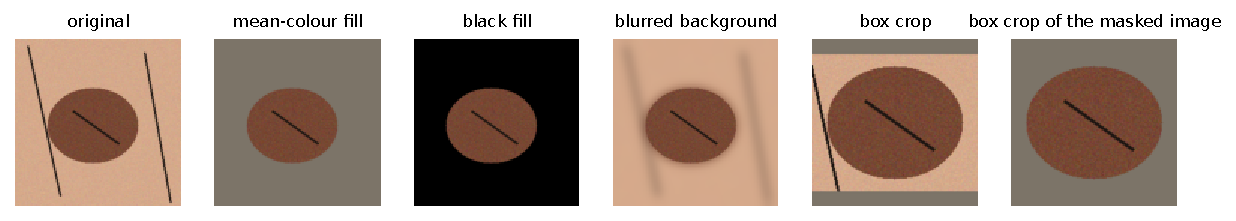
\includegraphics[width=\linewidth]{../stage7_robustness_external/figures/views_schematic.pdf}
\caption{The masking implementations of R8, illustrated on a synthetic image (a lesion with a hair-like line inside it
and two outside). No patient image is shown.}\label{s7:fig:views}\end{figure}
\paragraph{R9 --- dose-response over the real overlap} The artifact-bearing images of each cohort are binned by $r$:
$[0,0.1)$, $[0.1,0.3)$, $[0.3,0.5)$, $[0.5,0.75)$, $[0.75,1]$. Each bin is a trap with the cohort's shared artifact-free
group, built exactly like Trap~A and Trap~B. A bin with fewer than 25 images in any matched cell or fewer than 40
reversed-test positives is merged towards the middle of the $r$ range by a fixed rule. The primary endpoint is the
least-squares slope of $g_b$ on the bin's mean $r$, written as a linear combination of AUROCs so that the crossed bootstrap
gives the artifact-free images, which appear in every bin, one shared weight. H9: slope $<0$ in every cohort (Holm).
\paragraph{R10 --- ISIC 2019 $\to$ ISIC 2020} Train and validate on all \sSevenIsicTwoZeroOneNineTrainValImages{}
quality-controlled ISIC 2019 images (\sSevenIsicTwoZeroOneNineMelanomas{} melanomas) at their natural distribution; 5 seeds
of a group-safe 80/20 train/validation split. Test on every ISIC 2020 image \citep{rotemberg2021isic2020} with a lesion mask
(\sSevenIsicTwoZeroTwoZeroWithLesionMask) after removing near-duplicates of any ISIC 2019 image (perceptual hash, Hamming
distance $\le8$ --- the leakage rule of Stage~1): \sSevenTestImages{} images of \sSevenTestPatients{} patients,
\sSevenTestMelanomas{} melanomas. Lesion and hair masks are those of the Stage~5 external validation (models frozen before
any ISIC 2020 image was scored). In-lesion hair ($A$): hair on the lesion with $r\ge0.5$. Arms as in the natural test
sets of Stage~5 plus the remedies of Stage~6. Operating points OP1--OP5 use thresholds from each seed's ISIC 2019
validation predictions only. H10a: hard-pair AUROC mask $-$ ERM $<0$; H10b: at OP5 masking lowers sensitivity among
melanomas without in-lesion hair; H10c: group balancing beats masking on hard pairs.
\paragraph{R11 --- prospective theory test} The procedure of Stage~5, unchanged: for every cell (cohort $\times$ trap
or bin $\times$ arm) the two parameters $(S,A)$ are fitted to the clean and correlated AUROC, and the reversed AUROC --- and
every crossover, gain and slope built from it --- is predicted. The cells are the \sSevenTN{} R8 and R9 cells, none of which
existed when the rule was registered. Decision rule as in Stage~5: \emph{quantitatively predictive} only if every R8
crossover sign agrees, both correlations are $\ge0.7$ and the error beats ``reversed = clean''.

\subsection{Experiments}
\begin{table}[H]\centering\scriptsize
\caption{Experiments of this stage. One registration document (\texttt{docs/PREREGISTRATION\_ROUND4.md}) was committed before any feature, count or model of this stage existed. Commit times are set by the committing machine and are not independent proof of order.}\label{s7:tab:exp}
\begin{tabular}{p{3.6cm}p{3.2cm}p{2.8cm}p{5.4cm}}\toprule
Experiment & Status & First commit (local time) & Support criterion \\\midrule
R8 masking implementations (H8a, H8b) & \registered{round 4} & \texttt{d34b8b8}, 2026-09-28 11:28 & H8a: $C_v>0$ for black fill and box crop of the masked image in all four cohorts (Holm over 16) \\
R9 dose-response over the real overlap (H9) & \registered{round 4}; bin counts committed before fitting & \texttt{d34b8b8}, 2026-09-28 11:28 & slope of the mask gain on $r$ $<0$ in every cohort that passes the count gate (Holm) \\
R10 ISIC 2019 $\to$ ISIC 2020 natural test (H10a--c) & \registered{round 4} & \texttt{d34b8b8}, 2026-09-28 11:28 & hard-pair AUROC mask $-$ ERM $<0$; OP5 sensitivity loss; balancing $>$ mask on hard pairs \\
R11 prospective theory test (T1$'$--T3$'$) & \registered{round 4} & \texttt{d34b8b8}, 2026-09-28 11:28 & all crossover signs, $r\ge0.7$, MAE below ``reversed = clean'' \\
\bottomrule\end{tabular}
\end{table}


\subsection{Results}
\subsubsection{R8: the law does not depend on how masking is implemented}
Table~\ref{s7:tab:r8} and Figure~\ref{s7:fig:r8}. Every implementation gives a positive crossover in every cohort:
\sSevenNPrimOK{} of \sSevenNPrim{} tests are supported after Holm adjustment. For the full-removal views (H8a) this is
\sSevenHEightaN{} of \sSevenHEightaOf{}, so by the registered rule the law is \textbf{implementation-independent}. The
re-fitted mean-colour crossovers reproduce Stage~3 (dermoscopy \sSevenXisicmask, thyroid \sSevenXthyroidmask, capsule
\sSevenXcapsulemask, ovary \sSevenXovarymask).
\begin{table}[H]\centering\scriptsize
\caption{Location crossover $C_v$ for every masking implementation (DINOv2 ViT-B/14, crossed 95\% CIs). All 16 non-reference crossovers are positive with Holm-adjusted $p\le$ \sSevenHolmMax{} (family of 16).}\label{s7:tab:r8}
\resizebox{\linewidth}{!}{\begin{tabular}{lccccc}\toprule
Cohort & mean-colour fill (reference) & black fill & blurred background & box crop & box crop of the masked image \\\midrule
Dermoscopy hair (ISIC 2019) & $+0.147$ [$+0.111, +0.185$] & $+0.170$ [$+0.133, +0.207$] & $+0.154$ [$+0.117, +0.191$] & $+0.091$ [$+0.064, +0.117$] & $+0.154$ [$+0.121, +0.187$] \\
Thyroid calipers & $+0.239$ [$+0.196, +0.280$] & $+0.223$ [$+0.181, +0.265$] & $+0.218$ [$+0.177, +0.258$] & $+0.246$ [$+0.206, +0.285$] & $+0.250$ [$+0.210, +0.290$] \\
Capsule debris & $+0.377$ [$+0.328, +0.426$] & $+0.367$ [$+0.318, +0.416$] & $+0.278$ [$+0.221, +0.330$] & $+0.317$ [$+0.267, +0.367$] & $+0.358$ [$+0.305, +0.409$] \\
Ovary calipers & $+0.170$ [$+0.088, +0.250$] & $+0.153$ [$+0.063, +0.242$] & $+0.112$ [$+0.027, +0.195$] & $+0.145$ [$+0.083, +0.207$] & $+0.160$ [$+0.080, +0.240$] \\
\bottomrule\end{tabular}}
\end{table}

\begin{figure}[H]\centering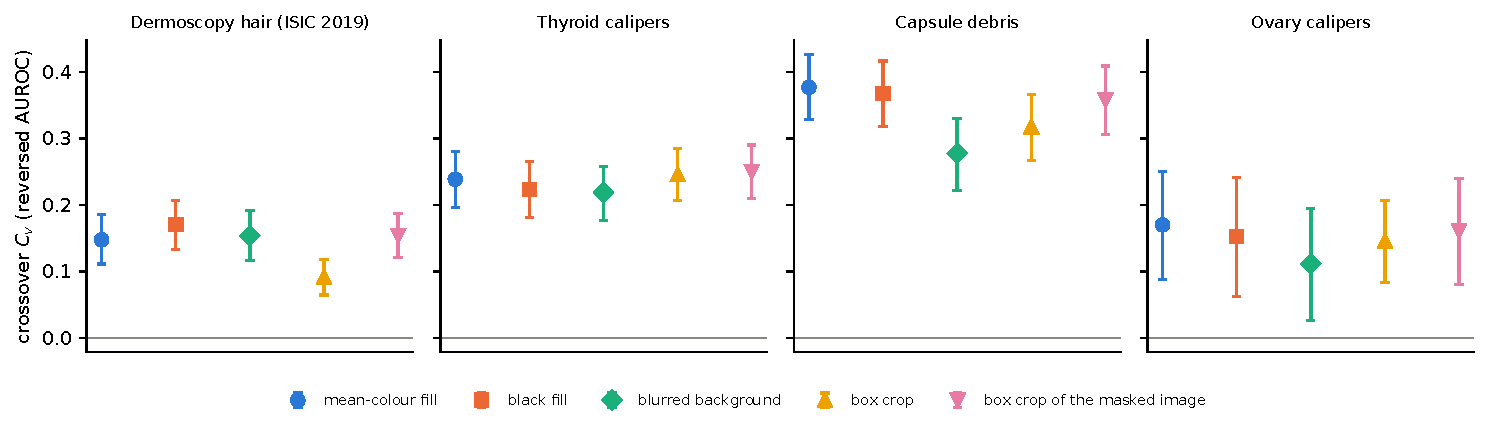
\includegraphics[width=\linewidth]{../stage7_robustness_external/figures/r8_crossover.pdf}
\caption{Crossover $C_v$ per masking implementation and cohort (crossed 95\% CIs). The reference (mean-colour fill) is
the leftmost point of each panel.}\label{s7:fig:r8}\end{figure}
\paragraph{Partial removal (H8b)} Both partial-removal views also give positive crossovers in every cohort
(\sSevenHEightbN{} of \sSevenHEightbOf), but they are weaker than mean fill only where the surviving content still
carries the artifact (Table~\ref{s7:tab:r8c}). The blurred background weakens the effect for capsule debris
(\sSevenCcapsulemaskblur) and ovarian calipers (\sSevenCovarymaskblur), not for hair (\sSevenCisicmaskblur): a 16-px blur
erases thin hair but leaves large debris recognisable. The box crop weakens it for hair (\sSevenCisiccropbox) and debris
(\sSevenCcapsulecropbox), whose out-of-ROI instances often lie next to the lesion and survive the crop, but not for
thyroid or ovarian calipers (\sSevenCthyroidcropbox, \sSevenCovarycropbox). The registered expectation ``partial removal
is weaker'' therefore holds in \sSevenHEightbConN{} of \sSevenHEightbConOf{} contrasts. One result was not expected: for hair, black fill gives a \emph{larger} crossover than mean fill
(\sSevenCisicmaskblack{} as $C_{\text{mask}}-C_v$).
\begin{table}[H]\centering\scriptsize
\caption{Secondary contrast $C_{\text{mask}}-C_v$: how much smaller the crossover of an implementation is than that of mean-colour fill (positive = weaker location effect than the reference).}\label{s7:tab:r8c}
\resizebox{\linewidth}{!}{\begin{tabular}{lcccc}\toprule
Cohort & black fill & blurred background & box crop & box crop of the masked image \\\midrule
Dermoscopy hair (ISIC 2019) & $-0.023$ [$-0.040, -0.007$] & $-0.006$ [$-0.042, +0.024$] & $+0.056$ [$+0.012, +0.099$] & $-0.007$ [$-0.033, +0.019$] \\
Thyroid calipers & $+0.016$ [$-0.004, +0.036$] & $+0.020$ [$-0.008, +0.049$] & $-0.007$ [$-0.049, +0.032$] & $-0.011$ [$-0.037, +0.014$] \\
Capsule debris & $+0.010$ [$-0.001, +0.021$] & $+0.099$ [$+0.067, +0.132$] & $+0.059$ [$+0.032, +0.087$] & $+0.019$ [$+0.001, +0.037$] \\
Ovary calipers & $+0.017$ [$-0.034, +0.079$] & $+0.058$ [$+0.004, +0.113$] & $+0.024$ [$-0.045, +0.096$] & $+0.010$ [$-0.046, +0.068$] \\
\bottomrule\end{tabular}}
\end{table}

\paragraph{What each implementation does in each trap} Figure~\ref{s7:fig:r8traps} and Table~\ref{s7:tab:r8t}. The pattern of
Stage~3 recurs for every implementation. For hair, every full-removal view harms inside the lesion (Trap~A: mean fill
\sSevenDisicmasktrapArev, black \sSevenDisicmaskblacktrapArev) and helps beside it (Trap~B: mean fill
\sSevenDisicmasktrapBrev). The views that keep some context harm less in Trap~A (blur \sSevenDisicmaskblurtrapArev, box
crop \sSevenDisiccropboxtrapArev) and gain less in Trap~B (box crop \sSevenDisiccropboxtrapBrev). For calipers and debris
every view still helps a little in Trap~A --- it removes clutter and overlays elsewhere on the screen (Stage~3) --- and
much more in Trap~B.
\begin{figure}[H]\centering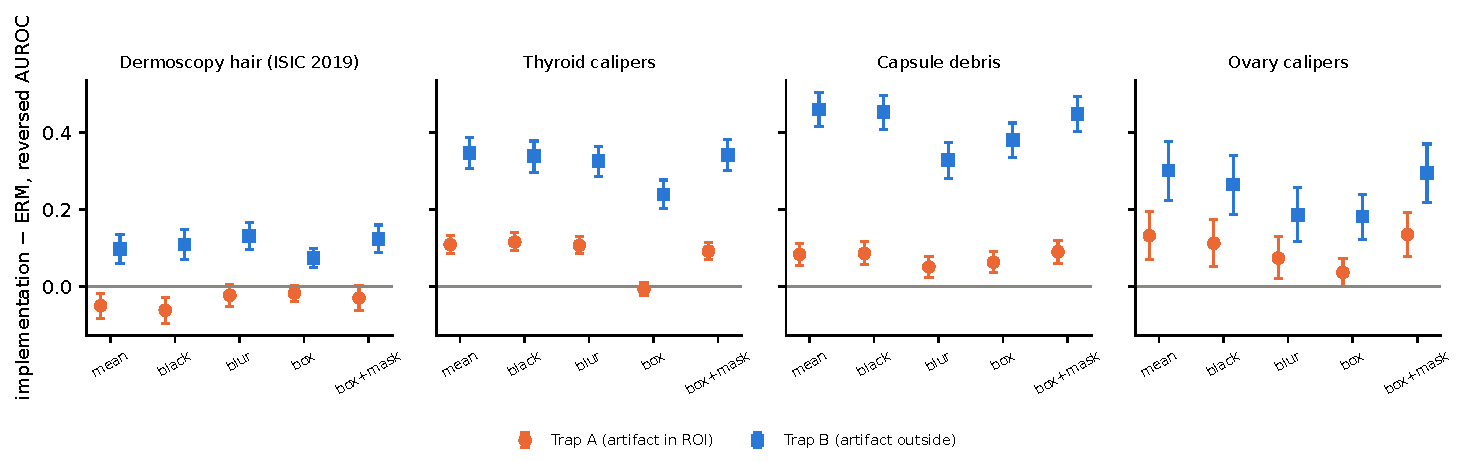
\includegraphics[width=\linewidth]{../stage7_robustness_external/figures/r8_traps.pdf}
\caption{Each implementation minus ERM on the reversed test, in Trap~A (artifact inside the ROI, orange circles) and
Trap~B (outside, blue squares); crossed 95\% CIs.}\label{s7:fig:r8traps}\end{figure}
\begin{table}[H]\centering\scriptsize
\caption{Each implementation minus ERM, per trap and test environment (AUROC, crossed 95\% CIs; descriptive).}\label{s7:tab:r8t}
\resizebox{\linewidth}{!}{\begin{tabular}{lccccc}\toprule
Cohort & Implementation & Trap~A reversed & Trap~B reversed & Trap~A clean & Trap~B clean \\\midrule
Dermoscopy hair (ISIC 2019) & mean-colour fill & $-0.049$ [$-0.083, -0.017$] & $+0.098$ [$+0.060, +0.136$] & $-0.023$ [$-0.045, -0.001$] & $-0.014$ [$-0.041, +0.014$] \\
 & black fill & $-0.061$ [$-0.097, -0.028$] & $+0.109$ [$+0.071, +0.148$] & $-0.028$ [$-0.052, -0.005$] & $-0.006$ [$-0.034, +0.022$] \\
 & blurred background & $-0.023$ [$-0.051, +0.005$] & $+0.131$ [$+0.096, +0.166$] & $-0.004$ [$-0.022, +0.014$] & $+0.020$ [$-0.006, +0.047$] \\
 & box crop & $-0.017$ [$-0.038, +0.003$] & $+0.074$ [$+0.049, +0.098$] & $-0.005$ [$-0.019, +0.009$] & $+0.010$ [$-0.007, +0.026$] \\
 & box crop of the masked image & $-0.030$ [$-0.062, +0.002$] & $+0.124$ [$+0.089, +0.160$] & $-0.010$ [$-0.030, +0.011$] & $+0.011$ [$-0.014, +0.035$] \\
Thyroid calipers & mean-colour fill & $+0.109$ [$+0.086, +0.133$] & $+0.348$ [$+0.307, +0.388$] & $+0.081$ [$+0.063, +0.100$] & $+0.166$ [$+0.118, +0.213$] \\
 & black fill & $+0.116$ [$+0.093, +0.140$] & $+0.339$ [$+0.297, +0.379$] & $+0.067$ [$+0.044, +0.089$] & $+0.171$ [$+0.125, +0.218$] \\
 & blurred background & $+0.107$ [$+0.086, +0.130$] & $+0.326$ [$+0.286, +0.365$] & $+0.065$ [$+0.044, +0.085$] & $+0.154$ [$+0.109, +0.199$] \\
 & box crop & $-0.006$ [$-0.023, +0.011$] & $+0.239$ [$+0.203, +0.277$] & $+0.015$ [$-0.003, +0.032$] & $+0.087$ [$+0.040, +0.135$] \\
 & box crop of the masked image & $+0.092$ [$+0.070, +0.115$] & $+0.342$ [$+0.303, +0.381$] & $+0.083$ [$+0.063, +0.101$] & $+0.174$ [$+0.129, +0.219$] \\
Capsule debris & mean-colour fill & $+0.084$ [$+0.055, +0.113$] & $+0.461$ [$+0.416, +0.506$] & $+0.064$ [$+0.044, +0.086$] & $+0.217$ [$+0.186, +0.251$] \\
 & black fill & $+0.086$ [$+0.056, +0.116$] & $+0.453$ [$+0.410, +0.497$] & $+0.063$ [$+0.044, +0.084$] & $+0.215$ [$+0.183, +0.248$] \\
 & blurred background & $+0.051$ [$+0.024, +0.077$] & $+0.329$ [$+0.282, +0.374$] & $+0.047$ [$+0.027, +0.068$] & $+0.156$ [$+0.129, +0.184$] \\
 & box crop & $+0.063$ [$+0.037, +0.090$] & $+0.381$ [$+0.336, +0.425$] & $+0.046$ [$+0.024, +0.068$] & $+0.174$ [$+0.145, +0.206$] \\
 & box crop of the masked image & $+0.091$ [$+0.060, +0.120$] & $+0.448$ [$+0.403, +0.494$] & $+0.056$ [$+0.033, +0.079$] & $+0.205$ [$+0.173, +0.238$] \\
Ovary calipers & mean-colour fill & $+0.132$ [$+0.071, +0.195$] & $+0.302$ [$+0.225, +0.378$] & $+0.055$ [$+0.014, +0.095$] & $+0.097$ [$+0.032, +0.159$] \\
 & black fill & $+0.113$ [$+0.053, +0.175$] & $+0.265$ [$+0.188, +0.342$] & $+0.028$ [$-0.013, +0.069$] & $+0.093$ [$+0.037, +0.149$] \\
 & blurred background & $+0.074$ [$+0.021, +0.130$] & $+0.186$ [$+0.116, +0.257$] & $+0.050$ [$+0.012, +0.086$] & $+0.065$ [$+0.014, +0.117$] \\
 & box crop & $+0.037$ [$+0.000, +0.072$] & $+0.182$ [$+0.122, +0.241$] & $+0.041$ [$+0.014, +0.068$] & $+0.078$ [$+0.038, +0.117$] \\
 & box crop of the masked image & $+0.135$ [$+0.078, +0.194$] & $+0.296$ [$+0.219, +0.371$] & $+0.050$ [$+0.007, +0.092$] & $+0.107$ [$+0.046, +0.167$] \\
\bottomrule\end{tabular}}
\end{table}


\subsubsection{R9: the location effect is graded}
Table~\ref{s7:tab:r9}, Table~\ref{s7:tab:r9b} and Figure~\ref{s7:fig:r9}. In every cohort the mask gain falls as more of the
artifact lies inside the ROI: slope \sSevenSlopeisic{} (hair), \sSevenSlopethyroid{} (thyroid), \sSevenSlopecapsule{}
(capsule) and \sSevenSlopeovary{} (ovary); \sSevenNHNine{} of \sSevenNHNineOf{} supported after Holm adjustment, with a
perfectly monotone ordering of the bins in every cohort. The two traps of Stages~3--6 are the ends of a continuous
dependence, not an artefact of the thresholds. For hair the gain passes through zero near $r=$ \sSevenZeroIsic{} and
becomes a harm when almost all of the hair lies on the lesion (\sSevenGisicbFive{} for $r\ge0.75$, against
\sSevenGisicbOne{} for $r<0.1$). For calipers and debris the gain shrinks several-fold (capsule
\sSevenGcapsulebOne{} $\to$ \sSevenGcapsulebFive; thyroid \sSevenGthyroidbOne{} $\to$ \sSevenGthyroidbFive) but stays
non-negative, for the reason given above: masking also removes on-screen clutter. The ovary cohort had too few images
with intermediate overlap and was analysed with three bins after the registered merge rule
(\sSevenBinsovary{} bins).
\begin{table}[H]\centering\scriptsize
\caption{Dose-response: least-squares slope of $g_b=$ rev(mask) $-$ rev(ERM) on the bin mean overlap $r$ (crossed 95\% CIs; the artifact-free images shared by all bins carry one bootstrap weight).}\label{s7:tab:r9}
\begin{tabular}{lcccccc}\toprule
Cohort & Bins & Slope of the mask gain on $r$ & Holm $p$ & Spearman & Zero crossing $r$ & H9 \\\midrule
Dermoscopy hair (ISIC 2019) & 5 & $-0.235$ [$-0.276, -0.194$] & $<0.001$ & -1.00 & 0.401 & \ok \\
Thyroid calipers & 5 & $-0.250$ [$-0.303, -0.197$] & $<0.001$ & -1.00 & none & \ok \\
Capsule debris & 5 & $-0.489$ [$-0.539, -0.438$] & $<0.001$ & -1.00 & none & \ok \\
Ovary calipers & 3 & $-0.205$ [$-0.300, -0.109$] & $<0.001$ & -1.00 & none & \ok \\
\bottomrule\end{tabular}
\end{table}

\begin{figure}[H]\centering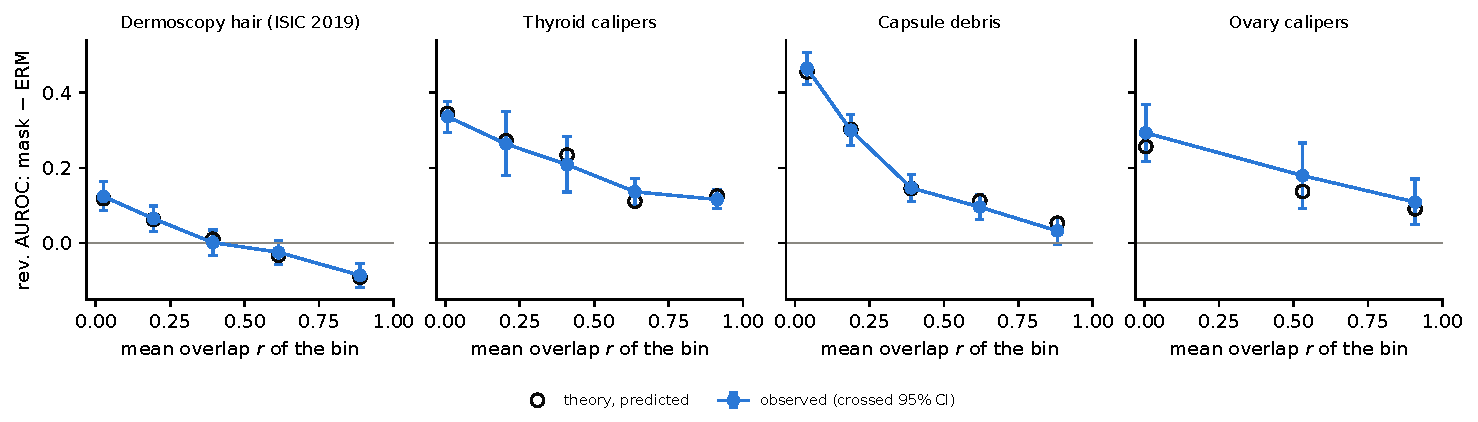
\includegraphics[width=\linewidth]{../stage7_robustness_external/figures/r9_dose.pdf}
\caption{Mask gain on the reversed test against the mean overlap $r$ of each bin (filled: observed, crossed 95\% CIs;
open: the theory's prediction from each bin's clean and correlated AUROC only).}\label{s7:fig:r9}\end{figure}
\begin{table}[H]\centering\scriptsize
\caption{Bins after the registered count gate ($\ge25$ per matched cell, $\ge40$ reversed-test positives over the folds of seed 42); merged bins are named by their parts. Cell counts are those of the matched pool.}\label{s7:tab:r9b}
\resizebox{\linewidth}{!}{\begin{tabular}{lccccccc}\toprule
Cohort & Bin & $r$ range & Mean $r$ & $A{=}1$: $Y{=}0$ / $Y{=}1$ & $A{=}0$: $Y{=}0$ / $Y{=}1$ & Rev.\ positives & Mask gain $g_b$ \\\midrule
Dermoscopy hair (ISIC 2019) & b1 & 0.00--0.10 & 0.026 & 4412 / 969 & 706 / 157 & 172 & $+0.124$ [$+0.085, +0.162$] \\
 & b2 & 0.10--0.30 & 0.194 & 3749 / 797 & 706 / 157 & 172 & $+0.065$ [$+0.029, +0.098$] \\
 & b3 & 0.30--0.50 & 0.393 & 2458 / 762 & 706 / 157 & 172 & $+0.001$ [$-0.034, +0.035$] \\
 & b4 & 0.50--0.75 & 0.614 & 1579 / 612 & 706 / 157 & 172 & $-0.025$ [$-0.057, +0.006$] \\
 & b5 & 0.75--1.00 & 0.888 & 1074 / 329 & 706 / 157 & 172 & $-0.086$ [$-0.119, -0.056$] \\
Thyroid calipers & b1 & 0.00--0.10 & 0.008 & 227 / 99 & 1052 / 749 & 829 & $+0.336$ [$+0.295, +0.377$] \\
 & b2 & 0.10--0.30 & 0.204 & 75 / 30 & 1052 / 749 & 300 & $+0.264$ [$+0.180, +0.349$] \\
 & b3 & 0.30--0.50 & 0.409 & 70 / 40 & 1052 / 749 & 400 & $+0.208$ [$+0.136, +0.283$] \\
 & b4 & 0.50--0.75 & 0.637 & 229 / 79 & 1052 / 749 & 790 & $+0.136$ [$+0.099, +0.172$] \\
 & b5 & 0.75--1.00 & 0.913 & 629 / 213 & 1052 / 749 & 829 & $+0.116$ [$+0.091, +0.141$] \\
Capsule debris & b1 & 0.00--0.10 & 0.041 & 231 / 1009 & 164 / 343 & 378 & $+0.465$ [$+0.422, +0.508$] \\
 & b2 & 0.10--0.30 & 0.188 & 391 / 769 & 164 / 343 & 378 & $+0.300$ [$+0.259, +0.343$] \\
 & b3 & 0.30--0.50 & 0.390 & 279 / 311 & 164 / 343 & 378 & $+0.147$ [$+0.111, +0.182$] \\
 & b4 & 0.50--0.75 & 0.621 & 237 / 227 & 164 / 343 & 378 & $+0.096$ [$+0.061, +0.130$] \\
 & b5 & 0.75--1.00 & 0.881 & 167 / 185 & 164 / 343 & 378 & $+0.032$ [$-0.004, +0.069$] \\
Ovary calipers & b1 & 0.00--0.10 & 0.004 & 91 / 103 & 170 / 178 & 196 & $+0.293$ [$+0.216, +0.369$] \\
 & b2b3b4 & 0.10--0.75 & 0.531 & 59 / 55 & 170 / 178 & 196 & $+0.179$ [$+0.091, +0.266$] \\
 & b5 & 0.75--1.00 & 0.909 & 298 / 244 & 170 / 178 & 196 & $+0.109$ [$+0.049, +0.170$] \\
\bottomrule\end{tabular}}
\end{table}


\subsubsection{R10: an external test at natural prevalence}
\paragraph{The data} After near-duplicate removal the test set has \sSevenTestImages{} images
(\sSevenTestMelanomas{} melanomas, \sSevenTestPatients{} patients). The removal was large: \sSevenDroppedNearDuplicates{}
images (\sSevenDropPct) were within Hamming distance 8 of an ISIC 2019 image --- \sSevenDupZerotoZero{} at distance 0,
\sSevenDupOnetoTwo{} at 1--2, \sSevenDupThreetoFive{} at 3--5 and \sSevenDupSixtoEight{} at 6--8 --- and it removed
melanomas less often (\sSevenDropMel) than benign lesions (\sSevenDropBen). Most removed images are therefore look-alikes
rather than copies (below). The association that masking can amplify is present
in both datasets: in-lesion hair on \sSevenHairisicTwoZeroOneNinemel{} of ISIC 2019 melanomas and
\sSevenHairisicTwoZeroOneNineben{} of benign lesions, and on \sSevenHairisicTwoZeroTwoZeromel{} and
\sSevenHairisicTwoZeroTwoZeroben{} in ISIC 2020.
\paragraph{AUROC} Tables~\ref{s7:tab:r10m} and \ref{s7:tab:r10b}, Figure~\ref{s7:fig:r10}. On all ISIC 2020 pairs masking
\emph{improves} the AUROC (\sSevenBmaskermall; ERM \sSevenNmermauc, mask \sSevenNmmaskauc) --- masking is the best arm by
overall AUROC. The improvement comes entirely from the shortcut-aligned pairs (\sSevenBmaskermeasy); on the
shortcut-conflicting pairs masking lowers the AUROC (\sSevenBmaskermhard; H10a \textbf{supported}, but only just: the upper
bound is \sSevenBhimaskerm). This is the Stage~5 signature --- right for the wrong reason on aligned cases, wrong on
conflicting ones --- on patients the model never saw, without any resampling. An external validation that reported only
the overall AUROC would recommend masking. Group balancing recovers the conflicting pairs (\sSevenBbalancedmaskhard{}
over mask; H10c \textbf{supported}) at a cost on aligned pairs (\sSevenBbalancedmaskeasy) and overall
(\sSevenBbalancedmaskall); combining masking with group balancing gives the highest cross-group AUROC
(\sSevenNmmaskbalancedcrossgroup, against ERM \sSevenNmermcrossgroup{} and mask \sSevenNmmaskcrossgroup).
\begin{table}[H]\centering\scriptsize
\caption{ISIC 2020 (external, natural prevalence), models trained on ISIC 2019: seed means. Hard pairs = melanomas without in-lesion hair vs benign lesions with it (they conflict with the training association).}\label{s7:tab:r10m}
\begin{tabular}{lccccc}\toprule
Arm & AUROC & Cross-group AUROC & AUROC, in-lesion hair & Hard pairs & Easy pairs \\\midrule
ERM & 0.791 & 0.772 & 0.779 & 0.772 & 0.798 \\
mask & 0.811 & 0.746 & 0.781 & 0.746 & 0.843 \\
balanced & 0.779 & 0.749 & 0.776 & 0.805 & 0.749 \\
mask + balanced & 0.792 & 0.776 & 0.777 & 0.786 & 0.783 \\
U-MtE & 0.799 & 0.752 & 0.783 & 0.752 & 0.827 \\
U-MtE balanced & 0.778 & 0.764 & 0.780 & 0.787 & 0.764 \\
U-MtE protect & 0.804 & 0.715 & 0.752 & 0.715 & 0.839 \\
U-MtE protect balanced & 0.790 & 0.753 & 0.747 & 0.753 & 0.789 \\
DFR & 0.765 & 0.730 & 0.746 & 0.782 & 0.731 \\
mask + DFR & 0.767 & 0.717 & 0.730 & 0.718 & 0.781 \\
JTT & 0.706 & 0.632 & 0.722 & 0.796 & 0.632 \\
\bottomrule\end{tabular}
\end{table}

\begin{table}[H]\centering\scriptsize
\caption{ISIC 2020: AUROC contrasts with crossed 95\% CIs (5 seeds; one Poisson weight per ISIC 2020 image).}\label{s7:tab:r10b}
\begin{tabular}{lccc}\toprule
Contrast & All pairs & Hard pairs & Easy pairs \\\midrule
mask $-$ ERM & $+0.020$ [$+0.003, +0.038$] & $-0.026$ [$-0.052, -0.000$] & $+0.045$ [$+0.005, +0.087$] \\
balanced $-$ mask & $-0.032$ [$-0.051, -0.014$] & $+0.059$ [$+0.035, +0.084$] & $-0.094$ [$-0.138, -0.051$] \\
U-MtE balanced $-$ mask & $-0.033$ [$-0.040, -0.026$] & $+0.041$ [$+0.030, +0.051$] & $-0.079$ [$-0.099, -0.059$] \\
U-MtE $-$ mask & $-0.012$ [$-0.018, -0.007$] & $+0.005$ [$-0.002, +0.013$] & $-0.016$ [$-0.029, -0.003$] \\
\bottomrule\end{tabular}
\end{table}

\begin{figure}[H]\centering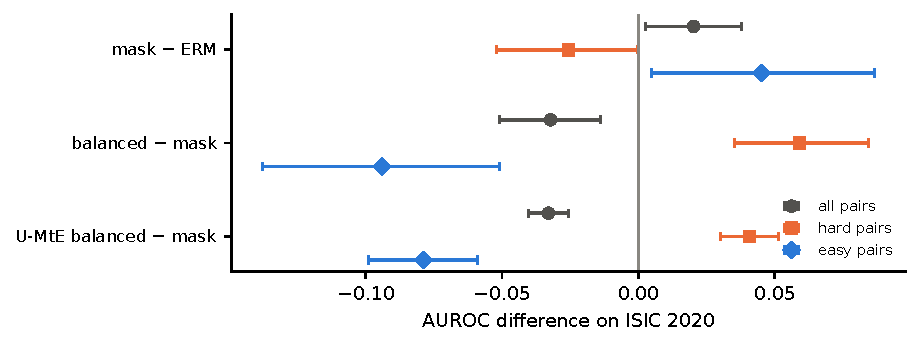
\includegraphics[width=0.75\linewidth]{../stage7_robustness_external/figures/r10_pairs.pdf}
\caption{ISIC 2020: AUROC differences on all, hard (shortcut-conflicting) and easy (shortcut-aligned) pairs; crossed
95\% CIs.}\label{s7:fig:r10}\end{figure}
\paragraph{Operating points} Table~\ref{s7:tab:r10op}. The AUROC effect does \emph{not} translate into a detectable
sensitivity loss at a fixed threshold: at OP5 (validation sensitivity $\ge0.90$) the sensitivity among melanomas without
in-lesion hair changes by \sSevenOpOPFiveconf{} (H10b \textbf{not supported}); at OP1 masking even raises sensitivity
without significance (\sSevenOpOPOnesens), and at OP2--OP4 it raises specificity (OP2 \sSevenOpOPTwospec). The clinical
consequence shown on the thyroid split of Stage~5 is therefore not reproduced here.
\begin{table}[H]\centering\scriptsize
\caption{ISIC 2020 operating points, mask $-$ ERM (crossed bootstrap with thresholds re-estimated on the weighted validation images in every replicate, 2{,}000 replicates).}\label{s7:tab:r10op}
\resizebox{\linewidth}{!}{\begin{tabular}{lccccc}\toprule
Operating point (threshold from ISIC 2019 validation) & Sensitivity ERM $\to$ mask & $\Delta$ sensitivity & $\Delta$ specificity & Sensitivity, melanomas without in-lesion hair & $\Delta$ \\\midrule
OP1 max.\ balanced accuracy & 0.434 $\to$ 0.516 & $+0.082$ [$-0.014, +0.167$] & $-0.003$ [$-0.046, +0.035$] & 0.432 $\to$ 0.519 & $+0.087$ [$-0.011, +0.168$] \\
OP2 specificity $\ge0.80$ & 0.472 $\to$ 0.477 & $+0.005$ [$-0.033, +0.052$] & $+0.029$ [$+0.017, +0.040$] & 0.470 $\to$ 0.482 & $+0.012$ [$-0.031, +0.063$] \\
OP3 specificity $\ge0.90$ & 0.309 $\to$ 0.324 & $+0.015$ [$-0.026, +0.062$] & $+0.016$ [$+0.009, +0.023$] & 0.309 $\to$ 0.332 & $+0.023$ [$-0.024, +0.072$] \\
OP4 sensitivity $\ge0.80$ & 0.523 $\to$ 0.545 & $+0.022$ [$-0.033, +0.077$] & $+0.021$ [$+0.002, +0.039$] & 0.524 $\to$ 0.547 & $+0.022$ [$-0.031, +0.079$] \\
OP5 sensitivity $\ge0.90$ & 0.702 $\to$ 0.699 & $-0.003$ [$-0.055, +0.052$] & $+0.028$ [$-0.011, +0.060$] & 0.700 $\to$ 0.693 & $-0.007$ [$-0.060, +0.047$] \\
\bottomrule\end{tabular}}
\end{table}


\subsubsection{R11: the theory predicts results it had not seen}
Table~\ref{s7:tab:r11} and Figure~\ref{s7:fig:r11}. Fitted only to each cell's clean and correlated AUROC, the theory's
predictions of the \sSevenTN{} held-out reversed AUROCs have a mean absolute error of \sSevenTMae{} (Pearson $r=$
\sSevenTR; \sSevenTWithin{} within 0.05), against \sSevenTMaeSym{} for the symmetric-reversal heuristic and
\sSevenTMaeClean{} for ``reversed = clean''. It gets the sign of all \sSevenTTwoN{} R8 crossovers right (\sSevenTTwoSign{} of
\sSevenTTwoN; $r=$ \sSevenTTwoR, MAE \sSevenTTwoMae), the sign of \sSevenTThreeSign{} of \sSevenTThreeN{} dose-response slopes
(MAE \sSevenTThreeMae) and of \sSevenTBinSign{} of \sSevenTBinN{} bin gains. By the registered rule the verdict is
\textbf{\sSevenTVerdict}. The difference from Stage~5's verdict (a qualitative account) is one of scope, not of rule:
Stage~5's cell set included chest radiographs, where one near-zero crossover had the wrong sign; the cells here are frozen
DINOv2 encoders with linear heads on four cohorts --- the setting the theory assumes.
\begin{table}[H]\centering\scriptsize
\caption{Prospective theory test: fitted to each cell's clean and correlated AUROC only; the reversed AUROC and every quantity derived from it are held out. None of these cells existed when the rule was registered.}\label{s7:tab:r11}
\begin{tabular}{lcccc}\toprule
Endpoint & Cells & Theory & ``reversed = clean'' & Symmetric reversal \\\midrule
T1$'$ reversed AUROC, all new cells & 84 & MAE 0.011, $r=$ 0.996 & MAE 0.177 & MAE 0.036 \\
T2$'$ R8 crossovers & 16 & signs 16/16, $r=$ 0.992, MAE 0.011 &  &  \\
T3$'$ R9 slopes & 4 & signs 4/4, MAE 0.018 &  &  \\
T3$'$ R9 bin gains & 18 & signs 18/18, MAE 0.014 &  &  \\
\bottomrule\end{tabular}
\end{table}

\begin{figure}[H]\centering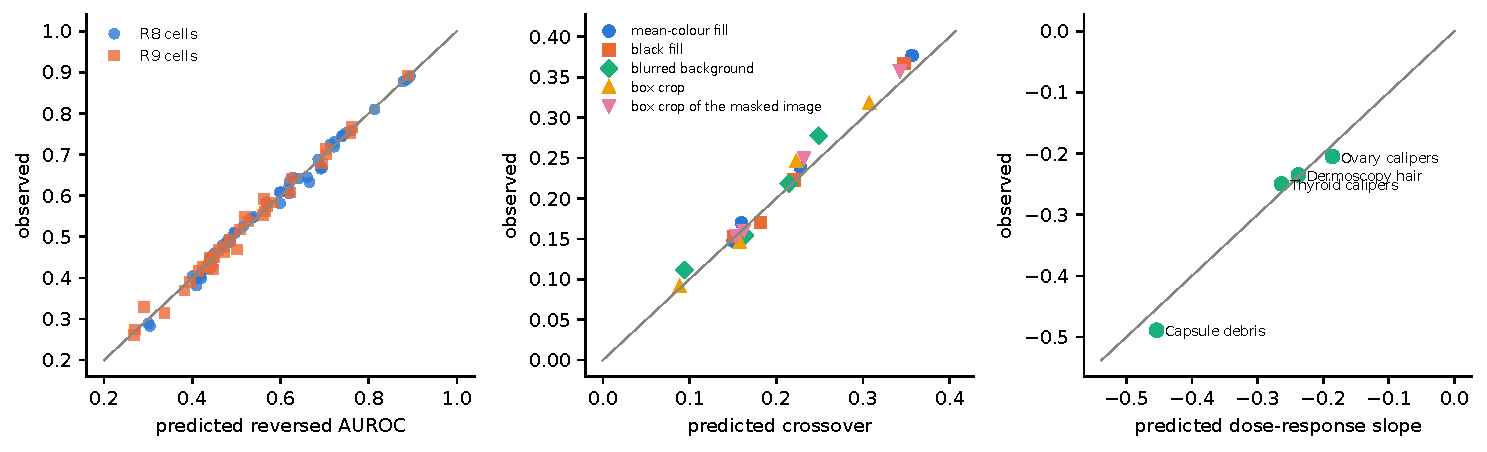
\includegraphics[width=\linewidth]{../stage7_robustness_external/figures/r11_theory.pdf}
\caption{Prospective test of the theory. Left: predicted versus observed reversed AUROC for every R8 and R9 cell. Middle:
R8 crossovers. Right: R9 dose-response slopes. Grey lines are the identity.}\label{s7:fig:r11}\end{figure}

\subsection{What failed or changed}
\begin{itemize}[leftmargin=*]\itemsep1pt
\item \textbf{H8b} holds in \sSevenHEightbConN{} of \sSevenHEightbConOf{} contrasts: partial removal is weaker than mean
fill for debris and ovarian calipers (blur) and for hair and debris (box crop), not otherwise; black fill gives a larger
hair crossover than mean fill.
\item \textbf{H10a} is supported by a margin that disappears at the third decimal; \textbf{H10b} is not supported: on
ISIC 2020 masking does not measurably lower sensitivity at a fixed operating point.
\item \textbf{Near-duplicate removal} discarded \sSevenDropPct{} of ISIC 2020. The rule was registered and uses no labels,
but \sSevenDupSixtoEight{} of the \sSevenDroppedNearDuplicates{} removed images are at distance 6--8, where a perceptual
hash also matches merely similar dermoscopy images, and melanomas were removed less often than benign lesions; the test
set is smaller than necessary, and a sensitivity analysis with a stricter distance was not run.
\item \textbf{The ovary} dose-response has only three bins.
\item \textbf{Scope}: R8--R10 use one encoder (DINOv2 ViT-B/14); R10 is dermoscopy only; the prospective theory test
covers frozen-encoder linear heads only.
\item No deviation from the registration. During the run only the execution was changed (parallel head fitting and
bootstraps, one BLAS thread per process, feature extraction in a separate process, batch size 128 for the new views);
data, seeds, models, estimands and bootstrap replicates are those registered, and the reproducibility gate was passed
exactly.
\end{itemize}

\subsection{Anticipated questions}
\paragraph{Why test several masking implementations if the theory already says what masking does?} Because the theory
treats masking abstractly (it lowers the disease signal and removes the out-of-ROI artifact signal). Real implementations
differ in what they leave behind --- a black border, blurred context, nearby pixels --- and a reviewer can reasonably
suspect that one of them escapes the law. None does.
\paragraph{Why does blur work as well as mean fill for hair but not for debris?} A 16-px Gaussian blur removes structures
a few pixels wide --- hair --- almost completely, so for hair it is effectively full removal. Capsule debris and bubbles
are large, low-frequency blobs that remain recognisable after blurring, so part of the out-of-ROI shortcut survives
(\sSevenCcapsulemaskblur{} weaker crossover).
\paragraph{Why is black fill stronger than mean fill for hair?} Not established. Black fill removes slightly more disease
context than mean fill inside Trap~A (clean AUROC \sSevenDisicmaskblacktrapAclean{} against \sSevenDisicmasktrapAclean{}) and
gains slightly more in Trap~B, which widens the crossover; why a black background does this for DINOv2 was not examined.
\paragraph{Why do the thyroid, capsule and ovary gains stay positive at $r\approx0.9$?} Masking removes more than the
artifact: on-screen annotations, scanner overlays and clutter outside the ROI also carry label information in the
training environment (Stage~3). The location law is about the part of the gain that the artifact's position controls, and
that part falls monotonically; for hair, where masking also removes disease context (Stage~2), the net gain becomes a harm.
\paragraph{Why is masking the best arm on ISIC 2020 by overall AUROC if it amplifies a shortcut?} Because the shortcut
agrees with the label in ISIC 2020 too: in-lesion hair is more common on melanomas. A model that relies more on in-lesion
hair gains on the many aligned pairs and loses on the fewer conflicting ones, and the aligned pairs dominate the overall
AUROC. This is exactly why the location law matters for external validation: the harm is invisible in the headline metric.
\paragraph{Why is the AUROC harm not visible at the operating points?} The hard-pair AUROC compares melanomas without hair
with benign lesions \emph{with} hair; a fixed threshold instead compares each melanoma with a threshold learned on ISIC
2019. Masking moved that threshold (specificity rises at OP2--OP4), and with \sSevenTestMelanomas{} melanomas the
sensitivity intervals are wide. On the thyroid split of Stage~5 the loss was large enough to show at every operating point;
on ISIC 2020 it is not.
\paragraph{Why were so many ISIC 2020 images removed, and does it matter?} The registered rule removes any ISIC 2020 image
within Hamming distance 8 of any ISIC 2019 image, the same threshold used to group near-duplicates for leakage-safe splits
(Stage~1). Dermoscopy images share a global layout (a central dark lesion on skin), so at distances 6--8 the hash also
matches different images. Only \sSevenDupZerotoZero{} removed images were exact
copies; \sSevenDupSixtoEight{} were at distance 6--8. The rule errs on the side of removing leakage and uses no labels, but
it removed melanomas less often than benign lesions (\sSevenDropMel{} against \sSevenDropBen), so it slightly raised the
melanoma share of the test set. Whether the hard-pair effect depends on it can be checked with a stricter distance.
\paragraph{Does the ``quantitatively predictive'' verdict replace Stage~5's ``qualitative account''?} No. Each verdict
belongs to its registered cell set. The defensible statement is: across all cohorts (Stage~5) the theory is a qualitative
account; for frozen-encoder linear heads on the four real-artifact cohorts it predicted \sSevenTN{} new cells
prospectively within \sSevenTMae{} AUROC and met the registered criterion.

\subsection{Conclusion}
\textbf{Supported.} The location crossover is independent of the masking implementation (\sSevenNPrimOK{} of \sSevenNPrim{} tests; H8a \sSevenHEightaN{} of \sSevenHEightaOf); it is
graded in the real overlap in all four cohorts (H9); on an external, patient-level test set at natural prevalence
masking lowers the AUROC on shortcut-conflicting pairs while raising it overall (H10a, borderline), and group balancing
recovers those pairs (H10c); the theory met its registered criterion for quantitative prediction on \sSevenTN{} prospective
cells. \textbf{Qualified.} Partial-removal views are weaker than mean fill in only \sSevenHEightbConN{} of \sSevenHEightbConOf{} contrasts (H8b), the
external AUROC harm is small, and near-duplicate removal was aggressive. \textbf{Not supported.} A sensitivity loss at a
fixed operating point on ISIC 2020 (H10b).

\subsection{Questions for the supervisor}
\begin{enumerate}\itemsep1pt
\item Should the masking-implementation result (R8) and the dose-response (R9) enter the main text, as the direct answers
to ``is mean fill a strawman?'' and ``are the traps hand-picked?''?
\item Is the ISIC 2020 result --- overall improvement, conflicting-pair harm, no operating-point effect --- best presented
as an argument for subgroup reporting in external validation rather than as a clinical harm?
\item May the paper now say that the theory \emph{predicts} for frozen-encoder linear probes, keeping ``qualitative
account'' for the full cell set?
\item Should the near-duplicate sensitivity analysis (a stricter hash distance) be run before submission?
\end{enumerate}


\clearpage
% generated by make_combined.py from stage8_labels_strong_model/stage8.tex; do not edit
\section{Stage 8 --- Are the real-artifact labels right, and does the law hold for a strong model?}\label{sec:stage8}

\stagebox{\textbf{In one sentence.} Checked without a clinician --- against three public expert annotation sets and two
independent automatic labellers --- the dermoscopy labels of Stage~3 put hair on the correct side of the lesion boundary
but mark hair on many images that experts call hair-free, and removing every image an independent source contradicts
\emph{increases} the crossover (\sEightOrigisic{} $\to$ \sEightCleanisic); the thyroid caliper labels agree with two
independent labellers wherever those agree with each other, but the registered cleaning rule removed too many images for
its test to run; the ovary and capsule labels could not yet be checked; and a fine-tuned thyroid model \sEightFTZeroGap{}
AUROC below the published benchmark shows every registered harm of masking, including a sensitivity loss from
\sEightConfErmOPTwo{} to \sEightConfMaskOPTwo{} in the \sEightSubN{} malignant nodules with a caliper on the nodule, a
subgroup now registered before any result.}
\subsection{Where this stage starts}
Stages~1--7 established the location law --- ROI masking removes an out-of-ROI shortcut and keeps, or amplifies, an
in-ROI one --- and showed that it holds across masking implementations, is graded in the real overlap and appears on an
external test set (Stage~7). Two objections remained that the earlier stages could not answer with their own data:
\begin{enumerate}[leftmargin=*]\itemsep1pt
\item \emph{``Nobody checked the real-artifact labels.''} The real traps of Stage~3 rest on automatic labels: published
hair masks \citep{wegley2026artifacts}, a rule-based caliper detector (thyroid, ovary), a contamination probe (capsule)
and lesion masks that are partly U-Net predictions. The audit package of Stage~6 was prepared for a clinician, and no
clinician is available to rate it.
\item \emph{``The thyroid model is weaker than published ones, and the subgroup was chosen after the fact.''} The frozen
probe of Stage~5 reaches a test AUROC of \sEightFrozenAuc{} on the official patient-disjoint split, below the fine-tuned
models of \citet{gong2022acl} (0.773--0.799); the \sEightSubN{} malignant nodules with an in-ROI caliper, in which masking
cost most sensitivity, were defined post hoc.
\end{enumerate}
This stage answers both with one registration (Part A: labels; Part B: a fine-tuned model), committed with three
amendments before any analysis.

\subsection{Questions}
\begin{enumerate}[label=\textbf{Q8\alph*},leftmargin=*]\itemsep1pt
\item How often do independent sources contradict our artifact labels, and do the errors differ by diagnosis?
\item Does the crossover survive on the images that no independent source contradicts?
\item Does a fine-tuned model close to the published benchmark show the harms that masking caused the frozen probe?
\item Does the subgroup harm hold when the subgroup is registered in advance?
\end{enumerate}
\paragraph{Design decisions} \emph{Why a clinician-free check is enough for these claims.} Whether a hair crosses a lesion,
a caliper lies on a nodule or debris lies inside a box is a visual fact, not a diagnosis, and the claims of Stage~3 need
only these facts. Moreover, if trap membership is misclassified independently of the diagnosis, the observed crossover is
attenuated, $C_{\text{obs}}\approx(1-e_A-e_B)\,C_{\text{true}}$: random label errors shrink a crossover and cannot create
one. The checks therefore measure the error rates, test whether they differ by diagnosis, and re-run the traps without the
contradicted images. \emph{Sources.} Public expert annotations where they exist: DermArtifactDB for hair presence
\citep{dermartifactdb}, IMA++ lesion masks \citep{imapp}, the hair masks of \citet{kabirhair} and expert contamination masks
for capsule frames \citep{capsulemasks}. No public caliper annotation exists, so two independent automatic labellers are
used for calipers: BUSClean, an ultrasound annotation detector \citep{busclean}, and MedGemma, a medical vision--language
model \citep{medgemma}, both run locally. \emph{Safeguards} (Amendments~1--2): images on which one of our own labellers was
trained are excluded from every comparison; a source is analysed only if it covers at least 200 of our images; a model
labeller counts only if its $\kappa$ is at least 0.40 on the images on which the two other caliper labels agree; BUSClean
is declared invalid if it fires on more than half of our caliper-free images; neither model labeller is ever shown our
artifact masks. \emph{Rating.} A blinded rating of the audit sample by the author (a non-clinician) is registered (A4);
it has not been done yet and does not enter the results below. \emph{Part B.} The recipe is chosen on validation images
only; the benchmark is the lowest published cross-entropy baseline on the same split (0.773).

\subsection{Methods}
\paragraph{A0 --- sources and coverage} Each source's licence was read from the source itself and recorded before use.
Matching: ISIC by image identifier; capsule frames by perceptual hash (Hamming distance $\le2$, as in Stage~1). IMA++ is
used as a majority mask over its annotators; its masks and anything derived from them at pixel level stay on the GPU
machine (CC BY-NC-ND). The coverage report was committed before any agreement was computed.
\paragraph{A1 --- agreement} Hair: $\kappa$ of our hair-free status ($\le30$ hair pixels) with DermArtifactDB; Dice of our
hair masks with the Kabir masks. Lesion masks: Dice with the IMA++ majority mask, and the trap class recomputed with it
(like for like at 518\,px). Calipers: $\kappa$ of presence with BUSClean and with MedGemma; for location, agreement of
our class with BUSClean's detected positions and with MedGemma's answer to ``is any caliper mark inside the green
contour?'' on the image with only the nodule outline drawn. MedGemma: fixed prompts, greedy decoding, answer parsed as
yes/no. Every agreement is reported for $Y=0$ and $Y=1$ separately.
\paragraph{A2 --- traps on uncontradicted labels} Contradicted images are removed; images without an independent source
are kept. The Stage~3 protocol is re-run unchanged (DINOv2 ViT-B/14 at 518\,px, same matching, seeds and folds, ERM and
mask arms, crossed bootstrap) with the count gate of Stage~7 ($\ge25$ images per matched cell). HA2: crossover $>0$ in
every cohort that passes the gate (Holm).
\paragraph{A3 --- differential error} Error rates of our cells against every informative source by trap and diagnosis;
differential error is flagged if the rates for $Y=1$ and $Y=0$ differ by more than 0.10 with a CI excluding zero, and a
flagged cohort's conclusion then rests on A2. The attenuation correction is reported only for unflagged cohorts.
\paragraph{Part B --- fine-tuned thyroid model} Twelve recipes (ConvNeXt-T, ResNet-50, DINOv2 ViT-B/14 $\times$ two
learning rates $\times$ 8 or 20 epochs; 224\,px, the training procedure of Stage~5) are compared by validation AUROC of
ERM, seed 42. The chosen recipe is then trained on the natural split (5 seeds $\times$ ERM, mask, balanced, mask +
balanced; validation predictions saved for the operating points) and in the thyroid traps (2 environment seeds $\times$ 5
folds = 10 bootstrap clusters). FT0 (descriptive): mean ERM test AUROC $\ge0.773$. FT1: hard-pair AUROC, mask $-$ ERM $<0$.
FT2: sensitivity CI below zero at $\ge3$ of OP2--OP5. FT3: at OP2, sensitivity of the malignant nodules with an in-ROI
caliper, mask $-$ ERM $<0$. FT4: trap crossover $>0$. Holm over FT1--FT4.
\paragraph{E1--E2 --- exploratory} Decided after A1--A3 were known and reported separately: a consensus view in which an
image counts as contradicted only if both caliper labellers place it in the same cell and that cell differs from ours
(E1), and FT3 restricted to the subgroup nodules that both labellers confirm (E2).

\subsection{Experiments}
\begin{table}[H]\centering\scriptsize
\caption{Experiments of this stage. \texttt{docs/PREREGISTRATION\_ROUND6.md} and its three amendments were committed before any analysis of this round; the coverage report (\sEightCommitCoverage), the fine-tune recipe (\sEightCommitRecipe) and the hash of the A4b key (\sEightCommitAfourb) were committed before the steps that use them. Commit times are set by the committing machine and are not independent proof of order.}\label{s8:tab:exp}
\begin{tabular}{p{3.8cm}p{3.4cm}p{2.8cm}p{5.0cm}}\toprule
Experiment & Status & First commit (local time) & Support criterion \\\midrule
A0 sources, licences, coverage & \registered{round 6}; coverage committed before A1 & \texttt{607900c}, 2026-09-28 14:27 & $\ge200$ matched images: analysed; 50--199: descriptive; $<50$: not feasible \\
A1 agreement with independent sources & \registered{round 6} & \texttt{607900c}, 2026-09-28 14:27 & descriptive; a model labeller is used only if $\kappa\ge0.40$ (Amendment 2: validity guard) \\
A2 traps on uncontradicted labels (HA2) & \registered{round 6}; primary of Part A & \texttt{607900c}, 2026-09-28 14:27 & crossover $>0$ in every cohort that passes the count gate (Holm) \\
A3 differential error, attenuation & \registered{round 6} & \texttt{607900c}, 2026-09-28 14:27 & flag: $|e_{Y=1}-e_{Y=0}|>0.10$, CI excluding 0; correction only for unflagged cohorts \\
A4 blinded rating by the author (A4b optional) & \registered{round 6}; not yet done & \texttt{607900c}, 2026-09-28 14:27 & intra-rater $\kappa$; error rates of our cells; judges a single model labeller (Amendment 2) \\
B1 fine-tune recipe (validation only) & \registered{round 6}; choice committed before B2 & \texttt{607900c}, 2026-09-28 14:27 & highest validation AUROC of 12 recipes \\
B2--B3 natural split and traps (FT0--FT4) & \registered{round 6} & \texttt{607900c}, 2026-09-28 14:27 & FT0 descriptive ($\ge0.773$); FT1--FT4 one-sided, Holm over four \\
E1--E2 consensus labels & \posthoc{exploratory; decided after A1--A3 were known} & --- & descriptive; not a test \\
\bottomrule\end{tabular}
\end{table}


\subsection{Results}
\subsubsection{Coverage}
Table~\ref{s8:tab:cov}. Five sources pass the coverage gate. IMA++ covers \sEightNIma{} of our dermoscopy images once the
\sEightImaExcl{} ISIC 2018 training images of our lesion U-Net are excluded. The capsule masks match \sEightCapBefore{} of
our frames, of which \sEightCapProbe{} trained our contamination probe and \sEightCapExpert{} already carry an expert mask
in Stage~3, leaving \sEightNCap: the capsule labels cannot be checked.
\begin{table}[H]\centering\scriptsize
\caption{Independent label sources and their coverage of our cohorts after the exclusions of Amendment~1 (training images of our own labellers). No image of the thyroid or ovary cohorts left the GPU machine: BUSClean and MedGemma ran locally.}\label{s8:tab:cov}
\begin{tabular}{p{2.2cm}p{3.2cm}p{3.4cm}p{2.4cm}p{1.6cm}p{1.6cm}}\toprule
Cohort & Source & Used for & Licence & Matched images & Gate \\\midrule
Dermoscopy hair & DermArtifactDB & hair present / absent & CC BY 4.0 & 20{,}519 & analysed \\
Dermoscopy hair & IMA{+}{+} & lesion masks, 1--5 annotators & cc-by-nc-nd-4.0 & 241 & analysed \\
Dermoscopy hair & Kabir hair masks & hair masks & CC BY 4.0 & 485 & analysed \\
Capsule debris & Multicentre clear/contaminated capsule masks & contamination masks & CC BY 4.0 & 29 & not feasible \\
Thyroid calipers & BUSClean & annotation detector (\texttt{detect\_anno}) & MIT & 3{,}493 & analysed \\
Ovary calipers & BUSClean & annotation detector (\texttt{detect\_anno}) & MIT & 1{,}202 & analysed \\
Thyroid calipers & MedGemma 1.5 4B-it & vision--language answers (presence, location) & model terms of use & 3{,}492 & analysed \\
Ovary calipers & MedGemma 1.5 4B-it & vision--language answers (presence, location) & model terms of use & 1{,}198 & analysed \\
\bottomrule\end{tabular}
\end{table}


\subsubsection{Dermoscopy hair: position right, presence over-called}
Table~\ref{s8:tab:isic}. \emph{Presence.} Agreement with DermArtifactDB is low, $\kappa=$ \sEightDermKappa, and the
disagreement is one-sided. Our artifact-free cell is clean: \sEightFreeOk{} of its \sEightNFreeDerm{} images are hair-free in
DermArtifactDB too. But our masks exceed the registered threshold of 30 hair pixels on \sEightFlagNeg{} of the
\sEightNDermNeg{} images DermArtifactDB calls hair-free (hair on \sEightOurHairPrev{} of images by our threshold, on
\sEightDermHairPrev{} by DermArtifactDB). Inside the traps DermArtifactDB reports no hair for \sEightDermNotrapA{} of Trap~A
and \sEightDermNotrapB{} of Trap~B images, more often for melanomas (Trap~A: \sEightDermNotrapAYOne{} against
\sEightDermNotrapAYZero; Trap~B: \sEightDermNotrapBYOne{} against \sEightDermNotrapBYZero). The difference is flagged as
differential error in both traps (\sEightDermDiffA{} and \sEightDermDiffB), so by the registered rule the dermoscopy
conclusion rests on A2.
\emph{Position.} Where hair is present, it is placed correctly. Our lesion masks agree with the IMA++ majority masks
(Dice \sEightImaDice), the trap class recomputed with IMA++ agrees for \sEightImaTrap{} of images, and IMA++ puts the hair
on the other side of the boundary for \sEightImaeA{} Trap-A and \sEightImaeB{} Trap-B images. Our hair masks overlap the
independent Kabir masks with Dice \sEightKabirDice{} --- thin structures, so pixel agreement is modest --- give the same
trap cell for \sEightKabirLocAgree{} of trap images and the opposite side for \sEightKabireA{} Trap-A and \sEightKabireB{}
Trap-B images. The measured location error $e_A+e_B$ is \sEightImaeSum{} (IMA++) and \sEightKabireSum{} (Kabir).
\begin{table}[H]\centering\scriptsize
\caption{Dermoscopy: agreement of our labels with three independent sources (95\% bootstrap CIs over images, 2{,}000 replicates). The Kabir images are all hair images and our masks mark hair on every one of them, so $\kappa$ is not informative there; the raw agreement is given instead.}\label{s8:tab:isic}
\resizebox{\linewidth}{!}{\begin{tabular}{lccccc}\toprule
Source & Quantity & Images & All & $Y=0$ (benign) & $Y=1$ (melanoma) \\\midrule
DermArtifactDB & hair present (ours: $>30$ hair pixels) & 20{,}519 & $\kappa$ 0.076 [0.070, 0.082] & $\kappa$ 0.083 [0.076, 0.090] & $\kappa$ 0.051 [0.041, 0.060] \\
IMA++ (majority mask) & lesion mask (Dice) & 241 & 0.851 [0.830, 0.870] & 0.851 [0.825, 0.872] & 0.853 [0.819, 0.888] \\
IMA++ & trap class ($r$ recomputed) & 239 & 0.841 [0.791, 0.887] & 0.855 [0.807, 0.899] & 0.750 [0.594, 0.875] \\
Kabir et al. & hair mask (Dice) & 485 & 0.618 [0.600, 0.637] & 0.617 [0.595, 0.638] & 0.629 [0.592, 0.665] \\
Kabir et al. & hair present & 485 & agreement \sEightKabirPresAgree &  &  \\
\bottomrule\end{tabular}}
\end{table}

\paragraph{Traps on uncontradicted labels} Removing the contradicted images (42\% of Trap~A, 43\% of Trap~B) raises the
crossover from \sEightOrigisic{} to \sEightCleanisic{} (Table~\ref{s8:tab:clean}, Figure~\ref{s8:fig:clean}; HA2 supported). This
is what attenuation predicts: images whose ``hair'' is not hair dilute the effect, and removing them sharpens it.
\begin{table}[H]\centering\scriptsize
\caption{Traps re-run on the images no informative source contradicts (A2; DINOv2 ViT-B/14, Stage~3 protocol, crossed 95\% CIs, Holm over the cohorts that ran). For capsule and ovary no image was removed, so the re-run reproduces Stage~3 and adds no evidence about the labels.}\label{s8:tab:clean}
\begin{tabular}{p{3.2cm}p{2.6cm}p{2.6cm}p{2.4cm}p{4.0cm}}\toprule
Cohort & Stage 3 crossover & Uncontradicted labels & Removed (Trap~A / Trap~B) & HA2 \\\midrule
Dermoscopy hair (ISIC 2019) & $+0.147$ [$+0.111, +0.185$] & $+0.199$ [$+0.164, +0.233$] & 42\% / 43\% & supported \\
Thyroid calipers & $+0.239$ [$+0.196, +0.280$] & --- & 61\% / 87\% & count gate not met (Trap~B) \\
Capsule debris & $+0.377$ [$+0.327, +0.426$] & $+0.377$ [$+0.327, +0.425$] & 0\% / 0\% & supported; nothing removed (no source analysable) \\
Ovary calipers & $+0.170$ [$+0.087, +0.252$] & $+0.170$ [$+0.089, +0.255$] & 0\% / 0\% & supported; nothing removed (no informative source yet) \\
\bottomrule\end{tabular}
\end{table}

\begin{figure}[H]\centering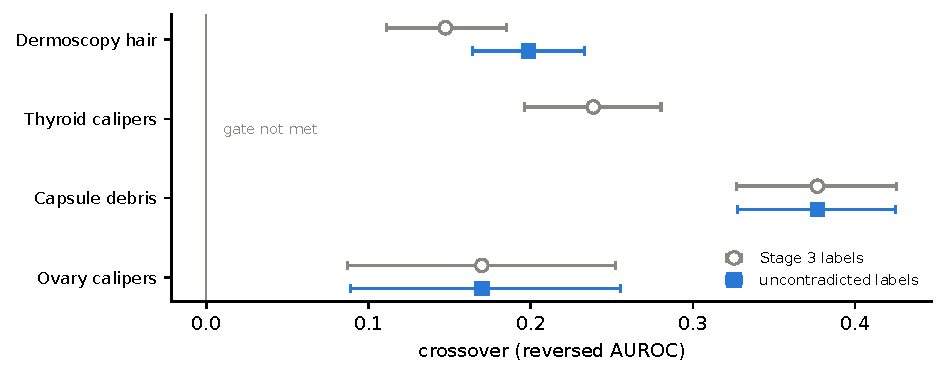
\includegraphics[width=0.8\linewidth]{../stage8_labels_strong_model/figures/cleaned.pdf}
\caption{Crossover on the Stage~3 labels (open circles) and on the images no informative source contradicts (squares),
crossed 95\% CIs. Capsule and ovary: nothing was removed; thyroid: the registered cleaning left too few Trap-B images.}
\label{s8:fig:clean}\end{figure}

\subsubsection{Thyroid calipers: two informative labellers with opposite biases}
BUSClean passes the validity guard (it fires on \sEightBusFreePos{} of our caliper-free images), and both labellers pass
the informativeness rule ($\kappa=$ \sEightBusInf{} and \sEightMgInf). Their presence agreement with our detector is
$\kappa=$ \sEightBusKappa{} (BUSClean) and \sEightMgKappa{} (MedGemma); location agreement is \sEightBusLoc{} on the
\sEightNBusLoc{} images where BUSClean returns positions and \sEightMgLoc{} on \sEightNMgLoc{} images for MedGemma.
Table~\ref{s8:tab:thylab} shows why the registered cleaning failed: the two labellers err in opposite directions. MedGemma
reports a caliper on \sEightMgYestrapA{} of our Trap-A images but also on \sEightMgYesartifactfree{} of our caliper-free
images; BUSClean rarely fires on caliper-free images but finds an annotation on only \sEightBusYestrapA{} of Trap-A images.
Under the registered rule --- remove an image if \emph{any} informative source disagrees --- the two biases add up:
\sEightContratrapA{} of Trap~A and \sEightContratrapB{} of Trap~B are removed, the cleaned Trap~B keeps \sEightGateBYZero{}
benign and \sEightGateBYOne{} malignant caliper images, below the gate of 25, and HA2 cannot be tested for thyroid.
\begin{table}[H]\centering\scriptsize
\caption{Thyroid: how often each independent labeller reports a caliper in each of our cells, and the share of images the registered rule removes (an image is removed if \emph{any} informative labeller places it in another cell).}\label{s8:tab:thylab}
\begin{tabular}{p{3.4cm}p{1.4cm}p{2.8cm}p{2.8cm}p{2.8cm}}\toprule
Our cell & Images & BUSClean: annotation found & MedGemma: caliper ``yes'' & Contradicted (registered rule) \\\midrule
caliper-free & 1{,}801 & 5\% & 29\% & 30\% \\
Trap~A (in the nodule) & 1{,}150 & 56\% & 99\% & 61\% \\
Trap~B (outside) & 326 & 37\% & 87\% & 87\% \\
\bottomrule\end{tabular}
\end{table}

\paragraph{Differential error} The measured location errors are $e_A=$ \sEightBuseA, $e_B=$ \sEightBuseB{} against BUSClean
and $e_A=$ \sEightMgeA, $e_B=$ \sEightMgeB{} against MedGemma. BUSClean's disagreement in Trap~A is smaller for malignant
nodules (\sEightBusDiffA), which is flagged; MedGemma's is not (\sEightMgDiffA{} and \sEightMgDiffB). The cohort is
therefore flagged and no attenuation correction is reported.
\paragraph{Where the two labellers agree (E1, exploratory)} Table~\ref{s8:tab:thycons}. BUSClean and MedGemma give the same
cell for \sEightNBoth{} of \sEightNCells{} images. On these, they agree with our cell for \sEightBothAgree: caliper-free
\sEightConsAgreeartifactfree, Trap~A \sEightConsAgreetrapA, Trap~B \sEightConsAgreetrapB. Counting an image as
contradicted only when both labellers agree against us removes \sEightConsContraartifactfree{} of caliper-free images,
\sEightConsContratrapA{} of Trap~A and \sEightConsContratrapB{} of Trap~B (\sEightConsContraBYZero{} of benign,
\sEightConsContraBYOne{} of malignant). Presence and in-nodule calipers are well supported; the weakest cell is Trap~B,
calipers outside the nodule. The trap re-run under this rule (E1) is prepared and has not been run.
\begin{table}[H]\centering\scriptsize
\caption{Thyroid, \textbf{exploratory}: the images on which BUSClean and MedGemma give the same cell. An image counts as contradicted only if both place it in the same cell and that cell differs from ours.}\label{s8:tab:thycons}
\begin{tabular}{p{3.4cm}p{2.4cm}p{2.0cm}p{2.0cm}p{1.4cm}p{1.4cm}}\toprule
Our cell & Both labellers agree with each other & \ldots\ and with our cell & Contradicted by both & benign & malignant \\\midrule
caliper-free & 1{,}301 & 97\% & 2\% & 2\% & 2\% \\
Trap~A (in the nodule) & 475 & 94\% & 2\% & 3\% & 1\% \\
Trap~B (outside) & 89 & 48\% & 14\% & 11\% & 21\% \\
\bottomrule\end{tabular}
\end{table}

\paragraph{The registered subgroup} Of the \sEightSubN{} malignant test nodules that our detector gives an in-ROI
caliper (FT3), no nodule is contradicted by both labellers, both confirm the caliper inside the nodule for
\sEightSubConfirmed, MedGemma places it inside for \sEightSubMgIn{} and never reports no caliper, and BUSClean finds no
annotation on \sEightSubBusNone. FT3 restricted to the doubly confirmed nodules (E2) is prepared and has not been run.

\subsubsection{Ovary calipers: one usable labeller}
BUSClean fails the validity guard: it fires on \sEightOvBusFreePos{} of our caliper-free ovary images, so on these screens
it detects on-screen annotation and text, not calipers, and is not used. MedGemma is the only labeller left; its presence
agreement with our detector is low, $\kappa=$ \sEightOvMgKappa{} (benign \sEightOvMgKappaYZero, malignant
\sEightOvMgKappaYOne), and at least one of the two is often wrong on these images. Which one is wrong is exactly what the
informativeness rule decides, and with a single model labeller the registered arbiter is the author's blinded rating
(Amendment~2), which has not been done. No ovary image is removed, and the A2 re-run reproduces Stage~3
(Table~\ref{s8:tab:clean}); it is not evidence about the labels.

\subsubsection{Capsule debris: not checkable}
With \sEightNCap{} matched frames the capsule comparison is not feasible by the coverage gate. All \sEightCapEmpty{}
expert masks of these frames mark no contaminated pixel, including the \sEightCapTrapCells{} frames our probe places in a
trap; with so few frames this is not interpreted. As for ovary, the A2 re-run reproduces Stage~3.

\subsubsection{Part B: a fine-tuned thyroid model near the benchmark}
\paragraph{Recipe} Table~\ref{s8:tab:recipe}. ConvNeXt-T (ImageNet-22k), learning rate \sEightLr, \sEightEpochs{} epochs had
the highest validation AUROC (\sEightValAuc; best DINOv2 ViT-B/14 recipe \sEightDinoVal) and was committed before the final
models were trained.
\begin{table}[H]\centering\scriptsize
\caption{Recipe selection on validation images only (B1); no test image was scored. The chosen recipe (bold) was committed before any final model was trained.}\label{s8:tab:recipe}
\begin{tabular}{lccc}\toprule
Architecture & Learning rate & Epochs & Validation AUROC (ERM, seed 42) \\\midrule
ConvNeXt-T (IN-22k) & 3e-5 & 8 & 0.849 \\
ConvNeXt-T (IN-22k) & 3e-5 & 20 & 0.842 \\
ConvNeXt-T (IN-22k) & 1e-4 & 8 & \textbf{0.865} \\
ConvNeXt-T (IN-22k) & 1e-4 & 20 & 0.865 \\
ResNet-50 & 3e-5 & 8 & 0.658 \\
ResNet-50 & 3e-5 & 20 & 0.723 \\
ResNet-50 & 1e-4 & 8 & 0.723 \\
ResNet-50 & 1e-4 & 20 & 0.781 \\
DINOv2 ViT-B/14 & 3e-5 & 8 & 0.838 \\
DINOv2 ViT-B/14 & 3e-5 & 20 & 0.850 \\
DINOv2 ViT-B/14 & 1e-4 & 8 & 0.715 \\
DINOv2 ViT-B/14 & 1e-4 & 20 & 0.804 \\
\bottomrule\end{tabular}
\end{table}

\paragraph{Hypotheses} Table~\ref{s8:tab:ft}. The mean ERM test AUROC is \sEightFTZero, \sEightFTZeroGap{} below the benchmark
of 0.773: by the registered rule the model is \emph{below benchmark}; the frozen probe reached \sEightFrozenAuc. All four tests are
supported after Holm adjustment. On shortcut-conflicting pairs masking lowers the AUROC by \sEightFTOne{} (FT1), while on
all pairs the change is \sEightConallmaskerm{} and on aligned pairs \sEightConeasymaskerm. Group balancing recovers the
conflicting pairs (balanced $-$ mask \sEightConhardbalancedmask), masking and balancing together do not
(\sEightConhardmaskbalancedmask). The trap crossover is \sEightFTFour{} (FT4).
\begin{table}[H]\centering\scriptsize
\caption{Part B: the chosen fine-tuned model on the official patient-disjoint thyroid split (5 seeds $\times$ 4 arms) and in the thyroid traps (10 bootstrap clusters). Crossed bootstrap; Holm over FT1--FT4.}\label{s8:tab:ft}
\begin{tabular}{lp{5.4cm}p{3.0cm}p{1.3cm}p{1.1cm}p{1.9cm}}\toprule
 & Hypothesis & Estimate [95\% CI] & $p$ (one-sided) & Holm $p$ & Verdict \\\midrule
FT0 & ERM test AUROC $\ge0.773$ (descriptive) & 0.769 & --- & --- & below benchmark \\
FT1 & hard-pair AUROC, mask $-$ ERM $<0$ & $-0.102$ [$-0.178, -0.026$] & 0.0040 & 0.0040 & supported \\
FT2 & sensitivity loss (CI $<0$) at $\ge3$ of OP2--OP5 & 4 of 4 & 0.0005 & 0.0015 & supported \\
FT3 & OP2 sensitivity, malignant with in-ROI caliper, mask $-$ ERM $<0$ & $-0.521$ [$-0.642, -0.382$] & 0.0005 & 0.0015 & supported \\
FT4 & thyroid trap crossover $>0$ & $+0.187$ [$+0.111, +0.268$] & 0.0001 & 0.0004 & supported \\
\bottomrule\end{tabular}
\end{table}

\paragraph{Operating points} Table~\ref{s8:tab:opft} and Figure~\ref{s8:fig:op}. Masking lowers sensitivity at every operating
point, at OP2 from \sEightSensErmOPTwo{} to \sEightSensMaskOPTwo{} (\sEightSensOPTwo), and raises specificity (from
\sEightSpecErmOPTwo{} to \sEightSpecMaskOPTwo): thresholds fixed on validation images land at a more conservative point on
the test set once the model is trained on masked images. In the registered subgroup of \sEightSubN{} malignant nodules with
a caliper on the nodule, sensitivity at OP2 falls from \sEightConfErmOPTwo{} to \sEightConfMaskOPTwo{} (\sEightFTThree;
FT3). This test was registered before any result of this model existed.
\begin{table}[H]\centering\scriptsize
\caption{Fine-tuned model, official patient-disjoint thyroid test split: masking at five validation-fixed operating points (crossed bootstrap, thresholds re-estimated in every replicate).}\label{s8:tab:opft}
\resizebox{\linewidth}{!}{\begin{tabular}{lccccc}\toprule
Operating point (fixed on validation) & Sensitivity ERM $\to$ mask & $\Delta$ sensitivity & $\Delta$ specificity & Sensitivity, malignant with in-ROI caliper (ERM $\to$ mask) & $\Delta$ in that subgroup \\\midrule
OP1 max.\ balanced accuracy & 0.781 $\to$ 0.408 & $-0.373$ [$-0.508, -0.243$] & $+0.239$ [$+0.155, +0.345$] & 0.779 $\to$ 0.269 & $-0.510$ [$-0.660, -0.346$] \\
OP2 specificity $\ge0.80$ & 0.747 $\to$ 0.371 & $-0.376$ [$-0.462, -0.297$] & $+0.225$ [$+0.163, +0.291$] & 0.744 $\to$ 0.223 & $-0.521$ [$-0.642, -0.382$] \\
OP3 specificity $\ge0.90$ & 0.542 $\to$ 0.218 & $-0.324$ [$-0.419, -0.228$] & $+0.143$ [$+0.098, +0.198$] & 0.526 $\to$ 0.108 & $-0.418$ [$-0.536, -0.276$] \\
OP4 sensitivity $\ge0.80$ & 0.783 $\to$ 0.423 & $-0.360$ [$-0.439, -0.257$] & $+0.232$ [$+0.159, +0.302$] & 0.779 $\to$ 0.267 & $-0.513$ [$-0.627, -0.371$] \\
OP5 sensitivity $\ge0.90$ & 0.888 $\to$ 0.646 & $-0.242$ [$-0.345, -0.162$] & $+0.240$ [$+0.159, +0.345$] & 0.867 $\to$ 0.510 & $-0.356$ [$-0.497, -0.225$] \\
\bottomrule\end{tabular}}
\end{table}

\begin{figure}[H]\centering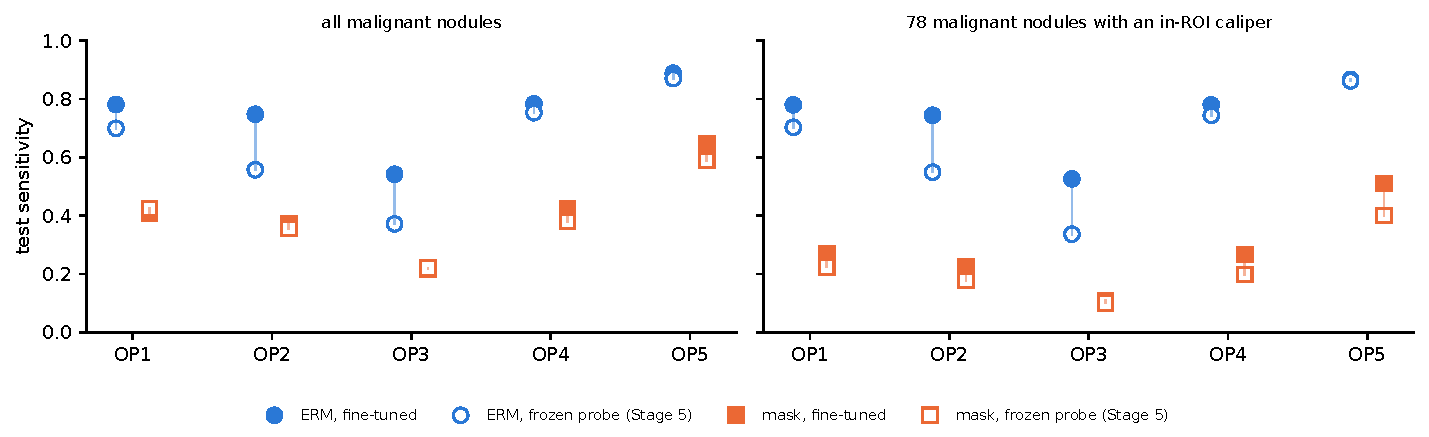
\includegraphics[width=\linewidth]{../stage8_labels_strong_model/figures/op_ft.pdf}
\caption{Test sensitivity of ERM (circles) and of the masked model (squares) at the five validation-fixed operating points,
for the fine-tuned model (filled) and the frozen probe of Stage~5 (open); left: all malignant nodules, right: those with a
caliper on the nodule. Thin lines join the two models.}\label{s8:fig:op}\end{figure}
\paragraph{Against the frozen probe} Table~\ref{s8:tab:cmp}. Every effect is at least as large for the stronger model: the
hard-pair harm (\sEightFrozenHard{} $\to$ \sEightFTOne), the OP2 sensitivity loss, and the subgroup loss
(\sEightFrozenConf{} $\to$ \sEightFTThree). The trap crossover is smaller than the frozen probe's (\sEightFrozenCross) and
larger than that of the fine-tuned ViT-S of Stage~5 (\sEightViTSCross).
\begin{table}[H]\centering\scriptsize
\caption{The same analyses for the frozen probe of Stage~5 and for the fine-tuned model of this stage. The subgroup was post hoc for the probe and registered in advance for the fine-tuned model.}\label{s8:tab:cmp}
\begin{tabular}{p{5.6cm}p{4.2cm}p{4.2cm}}\toprule
Quantity & Frozen DINOv2 ViT-B/14 probe (Stage~5) & Fine-tuned ConvNeXt-T (IN-22k) (this stage) \\\midrule
ERM test AUROC & 0.735 & 0.769 \\
Hard pairs, mask $-$ ERM & $-0.095$ [$-0.165, -0.022$] & $-0.102$ [$-0.178, -0.026$] \\
OP2 sensitivity, mask $-$ ERM & $-0.202$ [$-0.300, -0.100$] & $-0.376$ [$-0.462, -0.297$] \\
OP2 sensitivity, 78 malignant with in-ROI caliper & 0.549 $\to$ 0.177 & 0.744 $\to$ 0.223 \\
\quad change & $-0.372$ [$-0.499, -0.236$] & $-0.521$ [$-0.642, -0.382$] \\
Thyroid trap crossover & $+0.239$ [$+0.196, +0.280$] & $+0.187$ [$+0.111, +0.268$] \\
\bottomrule\end{tabular}
\end{table}


\subsection{What failed or changed}
\begin{itemize}[leftmargin=*]\itemsep1pt
\item \textbf{Hair presence.} The registered hair-free threshold ($\le30$ hair pixels) is far more sensitive than
DermArtifactDB's image-level label ($\kappa=$ \sEightDermKappa), about half of the trap images have no hair by
DermArtifactDB, and the disagreement differs by diagnosis. The hair position is right where hair exists.
\item \textbf{Thyroid HA2 not testable.} The registered ``any source'' rule removed \sEightContratrapB{} of Trap~B, because
the two caliper labellers err in opposite directions; the consensus analysis (E1) is exploratory.
\item \textbf{FT0} is missed by \sEightFTZeroGap{} AUROC: the fine-tuned model is near, not at, the benchmark.
\item \textbf{Capsule} labels could not be checked (\sEightNCap{} frames); \textbf{ovary} labels wait for the rating,
because BUSClean is invalid on ovarian screens. Their ``supported'' HA2 rows reproduce Stage~3 and are not new evidence.
\item \textbf{The rating} (A4, A4b) has not been done; E1 and E2 are prepared and have not been run.
\item \textbf{Reporting corrections after the run} (no estimate changed): the attenuation correction had been printed per
source even where another source of the same cohort flagged differential error, which A3 does not allow; it is now
withheld for both flagged cohorts (dermoscopy, thyroid). For thyroid the withdrawn MedGemma-based value would have been
more than 2.5 times the observed crossover, because $1-e_A-e_B$ is small when a noisy labeller is taken as the truth.
$e_A$ and $e_B$ against DermArtifactDB, which has no location information, had been printed as 0 and are now not defined.
$\kappa$ with the Kabir masks is not informative (our masks mark hair on all \sEightNKabir{} images) and is replaced by the
raw agreement. A committed smoke-test output was removed.
\end{itemize}

\subsection{Anticipated questions}
\paragraph{If DermArtifactDB finds no hair on half of the trap images, are the Stage~3 hair results wrong?} No. Those images
carry weak or no hair, so they dilute the trap; removing every contradicted image makes the crossover larger
(\sEightOrigisic{} $\to$ \sEightCleanisic), and the position of the hair, which is what the law is about, is confirmed
by two independent sources ($e_A+e_B\le$ \sEightImaeSum). The controlled experiments of Stages~2 and~4 place the artifact
themselves and do not use these labels at all.
\paragraph{How can $\kappa$ be so low if the artifact-free cell is almost perfectly clean?} Because the disagreement is
one-sided. Thirty native pixels are a short stretch of a single hair, or a dark line of the lesion, while DermArtifactDB
records whether hair is visible as an artifact. $\kappa$ is dominated by the many images we call hair-bearing and DermArtifactDB
calls hair-free.
\paragraph{Could the differential error have produced the crossover?} It cannot be ruled out from the error rates alone,
which is why the registered rule sends a flagged cohort to A2: without the contradicted images the crossover is larger,
not smaller.
\paragraph{Why did the thyroid cleaning fail if both labellers are informative?} ``Informative'' means $\kappa\ge0.40$, not
unbiased. MedGemma says ``yes'' too often and BUSClean too rarely; a rule that lets either one veto an image removes most
images whenever the two disagree, and they disagree most on calipers outside the nodule.
\paragraph{Is MedGemma a credible labeller?} It is a general medical vision--language model, not a caliper detector, and is
used only through the informativeness rule. Its answers are fixed-prompt, greedy and local, it never sees our masks, and it
is judged against other labels, not trusted: informative for thyroid, undecided for ovary, where its agreement with our
detector is low.
\paragraph{Why is the attenuation correction not reported?} The registration allows it only for cohorts without
differential error, and both cohorts with an informative source are flagged. The correction also treats the source as
the truth; with a noisy labeller it inflates the crossover rather than correcting it.
\paragraph{Is 0.769 ``benchmark-level''?} Not by the registered rule, which is 0.773. The paper can call the model
near-benchmark (\sEightFTZeroGap{} below the lowest published baseline, above the frozen probe) and must not call it
benchmark-level.
\paragraph{Why does sensitivity fall by half while the AUROC barely moves?} The AUROC compares rankings; the operating
points transport a threshold from validation to test. Training on masked images moves the model's test scores relative to
that threshold (specificity rises at every operating point), and the loss is largest in the malignant nodules whose
caliper, the retained shortcut, points to benign.
\paragraph{Why use exploratory analyses at all?} Because the registered rule failed for a structural reason that the
consensus view makes visible. E1 and E2 are reported apart from the registered results and are never tests.

\subsection{Conclusion}
\textbf{Supported.} Where an artifact is present, our labels put it on the correct side of the ROI boundary (dermoscopy,
two independent sources); the dermoscopy crossover survives, and grows, on uncontradicted labels (HA2); a fine-tuned model
near the benchmark shows every registered harm of masking --- on conflicting pairs (FT1), at every operating point (FT2),
in the subgroup of \sEightSubN{} malignant nodules with an in-ROI caliper, registered in advance (FT3), and in the traps (FT4).
\textbf{Qualified.} Hair presence is over-called, with errors that differ by diagnosis; thyroid caliper labels agree with
two independent labellers where those agree with each other, weakest for calipers outside the nodule, but the registered
cleaned-trap test could not run; the fine-tuned model is \sEightFTZeroGap{} below the benchmark. \textbf{Not yet known.}
Whether the ovary caliper labels are right, and the author's blinded rating; the capsule labels cannot be checked with
public data.

\subsection{Questions for the supervisor}
\begin{enumerate}\itemsep1pt
\item Is a clinician-free validation --- public expert annotations, two independent automatic labellers and a blinded
non-clinician rating --- acceptable for the paper, stated as such?
\item Should the paper lead with the cleaned dermoscopy crossover and report the over-called hair presence as a limitation
of the published hair masks at our threshold?
\item May the thyroid clinical result now be stated as registered (FT3), with the model described as near-benchmark?
\item Is the author's rating worth doing now, given that the ovary labels depend on it, or should the ovary real-artifact
evidence be presented as unvalidated?
\end{enumerate}


\clearpage

\section{Conclusion}\label{sec:conclusion}
\subsection{What the work shows}
\begin{enumerate}[leftmargin=*]\itemsep2pt
\item \textbf{Masking cannot remove what is inside the region of interest.} When only the artifact's position changes,
masking's benefit falls with its overlap with the ROI: in the controlled dermoscopy sweep from \sTwoMaskZero{} at no
overlap to \sTwoMaskOneZeroZero{} at full overlap (interaction \sTwoInter), and the interaction is positive in
\sTwoNInterPos{} of \sTwoNSweeps{} controlled sweeps across five modalities and four encoders (Stage~2). Whether the lost
benefit turns into harm depends on how much disease context masking also removes: it harms at full overlap in
\sTwoNHarmFull{} sweeps.
\item \textbf{The mechanism is retention with amplified reliance.} Occlusion alone does not harm; harm follows the
visibility of the artifact under mask dilation; and on the same images the masked model reacts to an in-ROI ruler about
\sTwoDpRatioFull{} times as strongly as ERM (\sTwoDpDiffFull). Masking removes the competing evidence and leaves the
in-ROI artifact as the strongest remaining predictor (Stage~2).
\item \textbf{The law holds for real artifacts.} With real hair, sonographer calipers and capsule debris, masking is
worth far less when the artifact lies inside the ROI: crossover positive in \sThreeNXPos{} of \sThreeNRuns{} cohort--encoder
pairs and in all four pre-specified location tests (Holm), with DINOv2, MedSigLIP and a CNN (Stage~3). Only for
dermoscopy hair does in-ROI masking actually harm; for calipers and debris it helps less.
\item \textbf{It is caused by location, not by which images carry the artifact.} The in-ROI and out-of-ROI images differ
strongly (SMD up to \sFourSmdBeforeCap), yet the crossover survives covariate matching and doubly robust adjustment in all
three feasible cohorts (thyroid \sFourAdjThy), and pasting the same real artifact inside or outside the ROI of the same
images reproduces the location effect in all four cohorts. A neutral paste reproduces most of that transplant effect,
which shows that \emph{any} label-correlated pattern inside the ROI defeats masking; the artifact's own content adds a
significant part for hair and calipers (Stage~4).
\item \textbf{It matters on unaltered data and at the bedside.} On unaltered test sets masking harms the
shortcut-conflicting cases in three of five (thyroid \sFiveNatthyroidhard); on the patient-disjoint thyroid split it lowers
sensitivity at every validation-fixed operating point (OP2 \sFiveSensOPTwo), most for malignant nodules with a caliper on
the nodule (\sFiveConfOPTwo; a post hoc subgroup, exploratory) (Stage~5). A fine-tuned model near the published
benchmark (test AUROC \sEightFTZero{} against 0.773) shows the same pattern with the subgroup registered in advance:
hard pairs \sEightFTOne, OP2 sensitivity in the subgroup \sEightFTThree, trap crossover \sEightFTFour. Most of the
operating-point loss comes from transporting validation thresholds; with each model's threshold re-tuned on the test set the
overall sensitivity is unchanged, and the conflicting subgroup still loses \sEightTMOne{} (registered) (Stage~8).
\item \textbf{It is general.} The crossover replicates at three model sizes (larger models exploit the in-ROI caliper
more), in fine-tuned networks, in the zero-shot scores of vision--language models, and on new patients (ISIC 2020,
\sFiveExtX) (Stage~5).
\item \textbf{It does not depend on how masking is done, and it is graded.} Black fill, a blurred background, a crop
to the lesion box and a crop of the masked image all give a positive crossover in all four real-artifact cohorts
(\sSevenNPrimOK{} of \sSevenNPrim, Holm); and the mask gain falls monotonically with the real overlap in all four
cohorts (slope for hair \sSevenSlopeisic), turning into harm for hair above $r\approx$ \sSevenZeroIsic{} (Stage~7).
\item \textbf{It is visible on external data at natural prevalence.} Trained on ISIC 2019 and tested on ISIC 2020, masking
leaves the overall AUROC nearly unchanged (\sSevenTcalibratedall) but lowers it on shortcut-conflicting pairs
(\sSevenTcalibratedhard{} under a label-free calibrated duplicate rule; \sSevenBmaskermhard{} under the looser registered rule).
The harm combines both halves of the law --- masking removes hair beside the lesion and keeps hair on it --- and a
sensitivity loss at a fixed operating point was not found (Stage~7).
\item \textbf{The real-artifact labels put the artifact on the correct side of the boundary.} Checked without a
clinician, the dermoscopy labels agree with two independent sources on where hair lies ($e_A+e_B\le$ \sEightImaeSum) but
mark hair on many images that experts call hair-free; removing every contradicted image raises the crossover from
\sEightOrigisic{} to \sEightCleanisic. Thyroid caliper labels agree with two independent labellers where those agree with
each other; the registered cleaned-trap test could not run for thyroid, and the ovary and capsule labels are not yet
checked (Stage~8).
\item \textbf{It is predictable.} A two-parameter linear-Gaussian model fitted to each model's clean and correlated
AUROC predicts the held-out reversed AUROC with mean error \sFiveTMae{} against \sFiveTMaeSym{} for the best heuristic, gets
every real-trap crossover sign right, and explains when masking harms (it removes disease context) and why the crossover
is always positive. Across all cohorts it is, by its pre-registered rule, a qualitative account and cannot see shortcuts
carried by correlates of the artifact (Stage~5); tested prospectively on \sSevenTN{} new frozen-encoder cells it met the
registered criterion for quantitative prediction (error \sSevenTMae) (Stage~7).
\item \textbf{What carries the shortcut decides the fix.} For frozen foundation-model features, the annotation-free U-MtE
repairs overlay-like in-ROI artifacts (thyroid Trap~A \sSixRemThyroidmte{} versus ERM, masking \sSixRemThyroidmask), needs
disease protection when the artifact resembles the pathology (capsule), and cannot help when the shortcut is carried by
correlates (hair, chest drains), where label-based reweighting is required. With image-level labels, U-MtE with balancing
or masking with DFR is the most robust choice. For fine-tuned networks, erasure must happen during training. On unaltered
data no remedy improves on masking uniformly (\sSixNatRemPos{} of \sSixNatRemN{} comparisons favour a remedy,
\sSixNatRemNeg{} favour masking) (Stage~6).
\end{enumerate}

\subsection{Contributions}
\begin{itemize}[leftmargin=*]\itemsep1pt
\item The \emph{location law} of ROI masking, stated as a crossover, shown under controlled overlap in five modalities and
with real artifacts in four diseases and three modalities, with chest radiography as a principled boundary.
\item Its mechanism (retention with amplified reliance), its causal identification on fixed images, and its clinical
consequence at validation-fixed operating points.
\item A closed-form account that matches held-out results, explains every regime observed and predicted new results
prospectively.
\item Robustness evidence: the law is independent of the masking implementation, graded in the real overlap, and visible
on an external test set in the shortcut-conflicting cases while the overall AUROC improves.
\item A decision guide for practitioners and an annotation-free remedy (U-MtE) with a public tool, tested against the
relevant published baselines.
\item A clinician-free validation of real-artifact labels against public expert annotations and independent
automatic labellers, with a registered rule for re-running the analyses on uncontradicted labels.
\item A methodological correction: the per-seed bootstrap inherited from the pilot understates uncertainty whenever
seeds share test images; the crossed estimator fixes it and is used throughout.
\end{itemize}

\subsection{Claims the work does not make}
\begin{itemize}[leftmargin=*]\itemsep1pt
\item That masking always harms in-ROI (it helps a little for calipers and debris).
\item That the theory predicts magnitudes in general (across all cohorts it is a qualitative account; the prospective
test that it passed covers frozen-encoder linear heads on four cohorts).
\item That masking causes a sensitivity loss on ISIC 2020 (it lowers the hard-pair AUROC, not the sensitivity at a fixed
operating point), or that the external harm is due to amplified in-lesion hair alone.
\item That U-MtE improves deployment performance (it does not on unaltered data), or works post hoc on fine-tuned networks.
\item That the transplant measures the harm of a particular real artifact (most of it is the paste).
\item That the cohorts without patient identifiers are patient-independent.
\item That the artifact labels are validated by a clinician (they are checked against public expert annotations and
automatic labellers), or that the fine-tuned thyroid model reaches the published benchmark (it is \sEightFTZeroGap{} below).
\end{itemize}

\subsection{Limitations and open work}
Artifact labels come from detectors and a probe; without a clinician they were checked against public expert
annotations and two automatic labellers (Stage~8), which confirmed the hair position, showed over-called hair presence and
left the ovary and capsule labels unchecked; the author's blinded rating is registered but not done. Three cohorts publish no patient identifiers. Reversed environments are constructed by subsampling.
Frozen linear probes are below published fine-tuned models on thyroid; the fine-tuned model of Stage~8 is near, not at,
the benchmark. External validation exists for dermoscopy only;
its registered near-duplicate rule was too loose and was replaced by a calibrated rule in a registered sensitivity
analysis. The robustness analyses of Stage~7 use one
encoder.
Some analyses could only be kept as point estimates. The open work before submission is the blinded rating, the
institutional confirmation of the submission statements, and the decisions on thesis structure listed at the end of
Stage~6.

\subsection{Take-home message}
Before masking an image to its region of interest to remove a shortcut, find out where the artifacts sit. If they sit
outside the ROI, masking works. If they sit inside it, masking keeps the artifact and removes everything that competed
with it, so the model relies on the artifact more; the remedy must then be chosen by what carries the shortcut --- the
artifact's pixels, a pathology-like appearance, or correlates of the artifact.

\bibliographystyle{plainnat}
\bibliography{../common/references}
\end{document}
